\documentclass[10pt, a4paper]{article}
\usepackage{graphicx}
\usepackage{amsmath, amssymb, amsthm}
\usepackage{mathrsfs}
\usepackage{geometry}
\usepackage{enumitem}
\usepackage{tikz, tcolorbox}
\usepackage{hyperref}
\usepackage{booktabs}
\usepackage{fullpage}
\usepackage{pgfplots}
\usepackage{multicol}
\usepackage[siunitx]{circuitikz}
\usepackage{caption}
\usepackage{float}
\usepackage{multirow}
\usepackage{polynom}
\usepackage{tikz-cd}
\usepackage[utf8]{inputenc}
\usepackage{pst-eucl}
\usepackage{tabu}
\usepackage{comment}
\usepackage{subcaption}
\usepackage{fancyvrb}
\usepackage{fancyhdr}
\usepackage{etoolbox}
\usepackage{fncychap}
\usepackage{setspace}
\usepackage{listings}
\usepackage{tkz-euclide}
\usepackage{parskip}
\usepackage{bookmark}
\usetikzlibrary{calc,intersections,decorations.pathreplacing, patterns, angles, quotes, cd, shapes, arrows, positioning, automata}
\usepgfplotslibrary{fillbetween}
\geometry{margin=1in}
\graphicspath{{./resources/images}}
\pgfplotsset{compat=newest}
\setlength\parindent{0pt} 

% Long Division for Polynomials
\makeatletter
\def\pld@CF@loop#1+{%
\ifx\relax#1\else
    \begingroup
    \pld@AccuSetX11%
    \def\pld@frac{{}{}}\let\pld@symbols\@empty\let\pld@vars\@empty
    \pld@false
    #1%
    \let\pld@temp\@empty
    \pld@AccuIfOne{}{\pld@AccuGet\pld@temp
        \edef\pld@temp{\noexpand\pld@R\pld@temp}}%
    \pld@if \pld@Extend\pld@temp{\expandafter\pld@F\pld@frac}\fi
\expandafter\pld@CF@loop@\pld@symbols\relax\@empty
\expandafter\pld@CF@loop@\pld@vars\relax\@empty
\ifx\@empty\pld@temp
    \def\pld@temp{\pld@R11}%
\fi
\global\let\@gtempa\pld@temp
\endgroup
\ifx\@empty\@gtempa\else
    \pld@ExtendPoly\pld@tempoly\@gtempa
\fi
\expandafter\pld@CF@loop
\fi}
\def\pld@CMAddToTempoly{%
    \pld@AccuGet\pld@temp\edef\pld@temp{\noexpand\pld@R\pld@temp}%
    \pld@CondenseMonomials\pld@false\pld@symbols
    \ifx\pld@symbols\@empty \else
        \pld@ExtendPoly\pld@temp\pld@symbols
    \fi
    \ifx\pld@temp\@empty \else
        \pld@if
        \expandafter\pld@IfSum\expandafter{\pld@temp}%
        {\expandafter\def\expandafter\pld@temp\expandafter
            {\expandafter\pld@F\expandafter{\pld@temp}{}}}%
        {}%
    \fi
    \pld@ExtendPoly\pld@tempoly\pld@temp
    \pld@Extend\pld@tempoly{\pld@monom}%
    \fi}
\makeatother

\newcommand{\QED}{\begin{flushright}\(\mathfrak{QED}\)\end{flushright}}
\newcommand{\Complex}{\mathbb{C}}
\newcommand{\Reals}{\mathbb{R}}
\newcommand{\Rationals}{\mathbb{Q}}
\newcommand{\Integers}{\mathbb{Z}}
\newcommand{\Naturals}{\mathbb{N}}
\newcommand{\rank}{\text{rank}}
\newcommand{\img}{\text{img}}
\newcommand{\geo}{\text{geo}}
\newcommand{\alg}{\text{alg}}
\newcommand{\Field}{\mathbb{F}}
\newcommand{\Prob}{\mathbb{P}}
\tikzstyle{terminator} = [rectangle, rounded corners, minimum width=3.5cm, minimum height=1cm, text centered, draw=black, fill=red!30]
\tikzstyle{decision} = [diamond, aspect=2, minimum width=3.5cm, text centered, draw=black, fill=blue!30, inner sep=1pt]
\tikzstyle{connector} = [draw, -latex']



\title{Mathematica Compendium}
\author{Miguel Antonio Méndez Hernández}
\date{\today}

\begin{document}

\maketitle

\newpage
\tableofcontents
\newpage
\newpage

\newpage
\subsection{Guidelines for Writing Formal Mathematical Proofs}

\textbf{General Principles}

\begin{itemize}
    
	\item \emph{Be precise:} use exact mathematical language and avoid vague statements.
   
	\item \emph{Be concise but complete:} do not skip logical steps that a knowledgeable reader needs.
    
	\item \emph{Explain your reasoning:} a proof is a logical explanation, not merely a chain of equations.
    
	\item \emph{Know your audience:} assume familiarity with definitions and standard theorems, but not your personal thought process.

\end{itemize}

\textbf{Structure of a Proof}

\begin{itemize}

	\item \emph{Begin with definitions and hypotheses:}  
    For a statement ``If \(P\), then \(Q\),'' start with ``Assume \(P\).''

    \item \emph{Direct proofs:} assume \(P\), derive consequences, and conclude \(Q\).

    \item \emph{Contrapositive proofs:} prove \(\neg Q \Rightarrow \neg P\) instead of \(P \Rightarrow Q\).

    \item \emph{Proof by contradiction:} assume the negation of the desired statement and derive a contradiction.

    \item \emph{Universal statements:} let an arbitrary object satisfying the hypothesis and show the statement holds for it.

    \item \emph{Existential statements:} construct an example or justify its existence, and verify the required properties.

    \item \emph{Equality of sets:} prove \(A \subseteq B\) and \(B \subseteq A\).

    \item \emph{Uniqueness proofs:} first show existence, then show any two such objects must be equal.

\end{itemize}

\textbf{Writing Style}

\begin{itemize}

	\item \emph{Write in complete sentences} with mathematical expressions integrated into the prose.
    
	\item \emph{Use transition words} such as ``therefore,'' ``hence,'' and ``thus'' to make logical flow explicit.
    
	\item \emph{Avoid informal symbols} such as arrows (\(\rightarrow\)) in prose except in formal logic contexts.
    
	\item \emph{Cite known theorems} when they are used in the argument.
    
	\item \emph{Keep notation consistent} throughout the proof.

\end{itemize}

\textbf{Using Definitions Explicitly.}

\begin{itemize}

	\item \emph{State relevant definitions clearly} when they are used.  
	For example, to prove continuity at \(a\), one begins:  
    ``Let \(\varepsilon > 0\). We must find \(\delta > 0\) such that \dots''

\end{itemize}

\textbf{Conclusion.}

\begin{itemize}
    \item \emph{End with a clear concluding statement} such as ``Therefore, \(Q\).'' or ``This completes the proof.''
\end{itemize}

\textbf{Common Mistakes to Avoid.}

\begin{itemize}

	\item \emph{Skipping logical steps} or jumping to conclusions.
    
	\item \emph{Using examples instead of general arguments.}
    
	\item \emph{Assuming the statement} you are trying to prove.
    
	\item \emph{Including irrelevant details.}
    
	\item \emph{Using ambiguous language} like ``clearly'' or ``obviously'' unless truly justified.

\end{itemize}

\textbf{Template.}

\begin{verbatim}
Proof.
[State assumptions clearly.]

[Develop argument using definitions and known theorems.]

[Use clear logical reasoning to reach the conclusion.]

Therefore, [claim to be proved].
\qed
\end{verbatim}

\newpage
\section{Propositional Logic}

Propositional logic is also called Boolean logic as 
it works on 0 and 1. In propositional logic, we use symbolic variables to represent the 
logic, and we can use any symbol for a representing a proposition, such 
\emph{A, B, C, P, Q, R}, etc. Propositions can be either \emph{true} \emph{false}, but it cannot be both.

\subsection{Logic Operators and Truth Tables}
\smallskip
\begin{multicols}{2}

	\subsection*{NOT (\(\neg\), \(\sim\))}

	\begin{tabular}{cc}
		\toprule
		\(A\) & \(\neg A\) \\
		\midrule
		0   & 1        \\
		1   & 0        \\
		\bottomrule
	\end{tabular}

	\vspace{1em}

	\subsection*{AND (\(\land\))}

	\begin{tabular}{ccc}
		\toprule
		\(A\) & \(B\) & \(A \land B\) \\
		\midrule
		0   & 0   & 0           \\
		0   & 1   & 0           \\
		1   & 0   & 0           \\
		1   & 1   & 1           \\
		\bottomrule
	\end{tabular}

	\vspace{1em}

	\subsection*{OR (\(\lor\))}

	\begin{tabular}{ccc}
		\toprule
		\(\)A\(\) & \(B\) & \(A \lor B\) \\
		\midrule
		0   & 0   & 0          \\
		0   & 1   & 1          \\
		1   & 0   & 1          \\
		1   & 1   & 1          \\
		\bottomrule
	\end{tabular}

	\vspace{1em}

	\subsection*{IMPLIES (\(\implies\))}

	\begin{tabular}{ccc}
		\toprule
		\(A\) & \(B\) & \(A \implies B\) \\
		\midrule
		0   & 0   & 1        \\
		0   & 1   & 1        \\
		1   & 0   & 0        \\
		1   & 1   & 1        \\
		\bottomrule
	\end{tabular}

	\columnbreak

	\subsection*{IFF (\(\iff\))}

	\begin{tabular}{ccc}
		\toprule
		\(A\) & \(B\) & \(A \iff B\) \\
		\midrule
		0   & 0   & 1         \\
		0   & 1   & 0         \\
		1   & 0   & 0         \\
		1   & 1   & 1         \\
		\bottomrule
	\end{tabular}

	\vspace{1em}

	\subsection*{XOR (\(\oplus\))}

	\begin{tabular}{ccc}
		\toprule
		\(A\) & $B$ & $A \oplus B$ \\
		\midrule
		0   & 0   & 0            \\
		0   & 1   & 1            \\
		1   & 0   & 1            \\
		1   & 1   & 0            \\
		\bottomrule
	\end{tabular}

	\vspace{1em}

	\subsection*{NOR (\(\downarrow\))}

	\begin{tabular}{ccc}
		\toprule
		\(A\) & \(B\) & \(A \downarrow B\) \\
		\midrule
		0   & 0   & 1                \\
		0   & 1   & 0                \\
		1   & 0   & 0                \\
		1   & 1   & 0                \\
		\bottomrule
	\end{tabular}

	\vspace{1em}

	\subsection*{NAND (\(\uparrow\))}

	\begin{tabular}{ccc}
		\toprule
		\(A\) & \(B\) & \(A \uparrow B\) \\
		\midrule
		0   & 0   & 1              \\
		0   & 1   & 1              \\
		1   & 0   & 1              \\
		1   & 1   & 0              \\
		\bottomrule
	\end{tabular}

\end{multicols}
\medskip

As a side not for the implication we can think about it as \emph{this, then}. Notice that 
only for the case \(1 \implies 0\) the output is false due to the fact this is a lie. For the other cases 
true and true is true, false and true is still true and false wit false is also true.

\subsection{Tautology and Contradiction}

\emph{Tautology}: A logical formula that is always true.

\emph{Contradiction}: A formula that is always false.

\subsection{Logical Equivalences}

\emph{Commutative Laws}

\[
	p \land q \iff q \land p \qquad p \lor q \iff q \lor p
\]

\emph{Associative Laws}

\[
	(p \land q) \land r \iff p \land (q \land r) \qquad (p \lor q) \lor r \iff p \lor (q \lor r)
\]

\emph{Distributive Laws}

\[
	p \land (q \lor r) \iff (p \land q) \lor (p \land r) \qquad
	p \lor (q \land r) \iff (p \lor q) \land (p \lor r)
\]

\emph{Identity Laws}

\[
	p \land \text{T} \iff p \qquad p \lor \text{F} \iff p
\]

\emph{Negation Laws}

\[
	p \lor \sim p \iff \text{T} \qquad p \land \sim p \iff \text{F}
\]

\emph{Double Negation Law}

\[
	\sim(\sim p) \iff p
\]

\emph{Idempotent Laws}

\[
	p \land p \iff p \qquad p \lor p \iff p
\]

\emph{Universal Bound Laws}

\[
	p \lor \text{T} \iff \text{T} \qquad p \land \text{F} \iff \text{F}
\]

\emph{De Morgan’s Laws}

\[
	\sim (p \land q) \iff (\sim p) \lor (\sim q) \qquad
	\sim (p \lor q) \iff (\sim p) \land (\sim q)
\]

\emph{Absorption Laws}

\[
	p \lor (p \land q) \iff p \qquad p \land (p \lor q) \iff p
\]

\emph{Conditional Laws}

\[
	(p \implies q) \iff (\sim p \lor q) \qquad \sim(p \implies q) \iff (p \land \sim q)
\]

\emph{Complement Law}

\[
	p \lor \neg p \iff \text{T} \qquad p \land \neg p \iff \text{F}
\]

\emph{Biconditional}

\[
	p \iff q \iff (p \implies q) \land (q \implies p)
\]

\emph{Transitivity}

\[
	(p \implies q) \land (q \implies r) \implies (p \Rightarrow r)
\]

\emph{Indirect Proof (Contrapositive)}

\[
	(p \implies q) \iff (\neg q \implies \neg p)
\]

\emph{Disjunctive Syllogism (Disjunctive Exclusion)}

\[
	p \nabla q \equiv (p \lor q) \land \neg p \implies q
\]

\[
	p \nabla q \equiv(p \land q) \lor \neg  (p \land q)
\]

\subsection{Truth Tables}

\emph{Truth tables} are a fundamental tool in logic that systematically show the truth value
(true or false) of a compound statement for every possible combination of the truth values of 
its individual component statements.

Essentially, they lay out all the scenarios and the resulting truth of the overall logical expression.
This helps determine if an argument is valid, if statements are logically equivalent, or the circumstances
under which a complex statement is true or false.

\textbf{Example:}

\begin{center}
	\begin{tabular}{|c|c|c|c|c|c|c|c|}
		\hline
		\(p\) & \(q\) & \(\neg p\) & \(\neg q\) & \(\neg p \implies q\) & \((\neg p \implies q) \land \neg p\) & \(\left[(\neg p \implies q) \land \neg p\right] \Rightarrow q\) \\
		\hline
		T   & T   & F        & F        & T                      & F                                     & T                                                                \\
		T   & F   & F        & T        & T                      & F                                     & T                                                                \\
		F   & T   & T        & F        & T                      & T                                     & T                                                                \\
		F   & F   & T        & T        & F                      & F                                     & T                                                                \\
		\hline
	\end{tabular}
\end{center}

\subsubsection{Filling a truth table}
To fill a truth table for a logical expression with truth values (True or False), you follow a 
specific order for the input variables. This order ensures that all possible combinations of truth values 
for the variables are covered.

\subsubsection{General Procedure:}

\begin{enumerate}

	\item \textbf{List all possible combinations of truth values for the input variables}: 
			If you have \(n\) variables, the number of rows in the truth table will be \(2^n\). Each 
			variable can be either True (T) or False (F).

	\item \textbf{Order of the input variables}:

			\begin{itemize}
					
				\item Start by filling in the truth values for the first variable. It alternates between 
					  True and False every \(2^{n-1}\) rows.
					
				\item Then for the second variable, it alternates every \(2^{n-2}\) rows, and so on.
					
				\item In short: the first variable alternates every other row, the second variable every two 
					rows, the third every four rows, and so on.
			
			\end{itemize}

\end{enumerate}

\textbf{Example: } 

For 3 variables, there are \(2^3 = 8\) possible combinations of truth values. The truth values are filled 
in the following order:

\[
	\begin{array}{|c|c|c|c|}
		\hline
		A & B & C & \text{Expression Result} \\
		\hline
		T & T & T &       -                  \\
		T & T & F &       -                  \\
		T & F & T &       -                  \\
		T & F & F &       -                  \\
		F & T & T &       -                  \\
		F & T & F &       -                  \\
		F & F & T &       -                  \\
		F & F & F &       -                  \\
		\hline
	\end{array}
\]

The pattern for filling the input truth values

\begin{itemize}

	\item The first column (A) alternates every 4 rows: `T, T, F, F, T, T, F, F`.

	\item The second column (B) alternates every 2 rows: `T, T, F, F, T, T, F, F`.

	\item The third column (C) alternates every row: `T, F, T, F, T, F, T, F`.

\end{itemize}

This ensures that all combinations of \(A\), \(B\), and \(C\) are covered, and you 
can then evaluate the logical expression for each combination.

\subsubsection{Truth Table for the Expression \texorpdfstring{\( (A \land B) \lor C \)}{}}

\[
	\begin{array}{|c|c|c|c|}
		\hline
		A & B & C & (A \land B) \lor C \\
		\hline
		T & T & T & T                  \\
		T & T & F & T                  \\
		T & F & T & T                  \\
		T & F & F & F                  \\
		F & T & T & T                  \\
		F & T & F & F                  \\
		F & F & T & T                  \\
		F & F & F & F                  \\
		\hline
	\end{array}
\]

\subsection{Disjunctive Normal Form (DNF)}

\emph{Disjunctive Normal Form (DNF)} is a standard way of writing a logical expression as a 
\emph{disjunction(OR)} of \emph{conjunctions (ANDs)}. A DNF expression consists of a series of
conjunctions of literals, where each conjunction is connected by disjunctions.

To find the DNF in a truth table take the rows of the final result where there are
true statements and bind the propositions that generated it with an AND inside parenthesis.
Repeat it with each of true rows and connect all parenthesis with OR's

\textbf{Example of DNF:}

Consider the logical expression:

\[
	(A \land B) \lor (\neg A \land C) \lor (B \land \neg C)
\]

This is in DNF because it is a disjunction (OR) of conjunctions (ANDs) of literals.

\subsection{Conjunctive Normal Form (CNF)}

\emph{Conjunctive Normal Form (CNF)} is a standard way of writing a logical expression as a 
\emph{conjunction (AND)} of \emph{disjunctions (ORs)}. A CNF expression consists of a series of 
disjunctions of literals, where each disjunction is connected by conjunctions.

To find the CNF proceed just as the DNF but with the false rows and instead
of ANDs inside the parenthesis use OR and connect the terms with OR\@. 
Also add a negation before each parenthesis.

\textbf{Example of CNF:}

Consider the logical expression:

\[
	\neg (A \lor B) \land \neg (\neg A \lor C) \land \neg (B \lor \neg C)
\]

This is in CNF because it is a conjunction (AND) of disjunctions (ORs) of literals.

\subsection{Basis}

A \emph{Basis} in the field of logic is set of operations with which you can 
represent all possible logic operations.

\textbf{Example:} The set \(\{ \lnot, \land\}\)

\subsection{Karnaugh Maps}

\emph{Karnaugh Maps (K-Maps)} are a graphical method used to simplify Boolean expressions. 
The main goal of a K-map is to group adjacent cells that contain 1's in order to simplify the expression. 
A K-map helps identify common terms, allowing the Boolean expression to be reduced to its simplest form.

\subsubsection{Karnaugh Map for Two Variables}

Consider the Boolean expression \( (A \lor (B \land \neg A \land \neg B)) \).

We first construct a K-map for two variables, \(A\) and \(B\). The truth table for this expression 
gives the following values:

\[
	\begin{array}{|c|c|c|}
		\hline
		A & B & (A \lor (B \land \neg A \land \neg B)) \\
		\hline
		0 & 0 & 0                                      \\
		0 & 1 & 1                                      \\
		1 & 0 & 1                                      \\
		1 & 1 & 1                                      \\
		\hline
	\end{array}
\]

The corresponding K-map is:

\[
	\begin{array}{|c|c|c|c|c|}
		\hline
		AB           & 00 & 01 & 11 & 10 \\
		\hline
		\text{Value} & 0  & 1  & 1  & 1  \\
		\hline
	\end{array}
\]

Here, we group the ones together to simplify the Boolean expression. The simplified expression is:

\[
	A \lor B
\]

\subsubsection{Karnaugh Map for Three Variables}

Now, let's consider the expression \( \neg C \). This expression only 
depends on one variable, but for illustration, we will use a 
3-variable K-map with variables \(A\), \(B\), and \(C\).

The truth table for \( \neg C \) is as follows:

\[
	\begin{array}{|c|c|c|c|}
		\hline
		A & B & C & \neg C \\
		\hline
		0 & 0 & 0 & 1      \\
		0 & 0 & 1 & 0      \\
		0 & 1 & 0 & 1      \\
		0 & 1 & 1 & 0      \\
		1 & 0 & 0 & 1      \\
		1 & 0 & 1 & 0      \\
		1 & 1 & 0 & 1      \\
		1 & 1 & 1 & 0      \\
		\hline
	\end{array}
\]

The corresponding K-map for three variables \(A\), \(B\), and \(C\) is:

\[
	\begin{array}{|c|c|c|c|}
		\hline
		AB \backslash C & 0 & 1 \\
		\hline
		00              & 1 & 0 \\
		01              & 1 & 0 \\
		11              & 1 & 0 \\
		10              & 1 & 0 \\
		\hline
	\end{array}
\]

We see that the ones are grouped in a column, leading to the simplified Boolean expression:

\[
	\neg C
\]

\subsubsection{Solving a Karnaugh Map}

To solve a Karnaugh Map and simplify a Boolean expression, follow these steps:

\begin{enumerate}
	
	\item \textbf{Determine the Number of Variables:} Decide how many variables are in the 
		   Boolean function. This determines the size of the K-Map:
	      
		\begin{itemize}
		 
			\item 2 variables: \(2 \times 2\)
		 	
			\item 3 variables: \(2 \times 4\)
		 
			\item 4 variables: \(4 \times 4\)
		 
			\item etc.
	  
		\end{itemize}

	\item \textbf{Fill in the K-Map:} Place 1's in the cells that correspond to the min-terms 
		  (where the function outputs 1). You may also include do not care conditions 
		  (usually denoted as \(X\)).

	\item \textbf{Group the 1's:} Form groups (called \emph{implicants}) of 1's. 
		   The groups must follow these rules:
	      
		\begin{itemize}
		 
			\item Each group must contain \(1, 2, 4, 8, \ldots\) (powers of 2) 1's.
		 
			\item Groups must be rectangular (e.g., \(1 \times 2\), \(2 \times 2\)).
		 
			\item Groups can wrap around the edges of the K-Map.
		 
			\item Try to form the largest groups possible to simplify the expression.
		 
			\item Each 1 should be included in at least one group.
	 
		\end{itemize}

	\item \textbf{Write the Simplified Expression:} \\
	      For each group:

		  \begin{itemize}

			\item Identify the variables that are constant (either always 0 or always 1) across the group.

			\item Write a product term (AND) using only the constant variables.

			\item Combine all product terms with OR operations to get the final simplified SOP (Sum of 
				  Products) expression.

		\end{itemize}

	\end{enumerate}

\subsection{Mathematical Quantifiers}

\subsubsection{Universal Quantifier \texorpdfstring{\(\forall\)}{}}  

Means \textbf{``for all''} or \textbf{``for every''}.

{Negation:} \(\neg (\forall x)\,P(x) \equiv (\exists x)\, \neg P(x)\) ``Not all'' is the same as 
``There exists one that does not''.

\textbf{Example:} 

\(\forall x \in \Reals,\ x^2 \geq 0\) For all real numbers, the square is greater than or equal to zero.

\textbf{Negated Example:} 

\(\exists x \in \Reals,\ x^2 < 0\) There exists a real number whose square is less than zero — this is 
false.

\subsubsection{Existential Quantifier \texorpdfstring{\(\exists\)}{}}  
	
Means \textbf{``there exists at least one''}.
 		
\emph{Negation:}  \(\neg (\exists x)\,P(x) \equiv (\forall x)\, \neg P(x)\) ``There does not exist'' is 
the same as ``For all, not''.

\textbf{Example:} 

\(\exists x \in \Naturals,\ x > 10\) There exists a natural number greater than 10.
			
\textbf{Negated Example:}  

\(\forall x \in \Naturals,\ x \leq 10\) All natural numbers are less than or equal to 10 — this is false.

\subsubsection{Unique Existential Quantifier \texorpdfstring{\(\exists ! \)}{}} 
	
Means \textbf{``there exists exactly one''}.
		
\emph{Negation:} ``Not exactly one'' means:
\(\neg (\exists! x)\, P(x) \equiv (\forall x)\, \neg P(x)\ \lor\ (\exists x_1 \neq x_2)\, P(x_1) \land 
P(x_2)\) Either no such \(x\) exists, or more than one does.

\textbf{Example:} 

\(\exists! x \in \Reals,\ x + 5 = 0\) There exists exactly one real number such that \( x + 5 = 0 \).

\textbf{Negated Example:}  

\(\exists x_1 \neq x_2 \in \Reals,\ x_1^2 = 4 \land x_2^2 = 4\) There are multiple solutions to 
\( x^2 = 4 \).

\subsection{Common Symbols Used in Mathematical Expressions}

\begin{itemize}

	\item \(>\)  (greater than)

	\item \(<\)  (less than)

	\item \(\geq\)  (greater than or equal to)

	\item \(\leq\)  (less than or equal to)

	\item \(=\)  (equals)

	\item \(\neq\)  (not equal)

	\item \(\in\)  (element of a set)

	\item \(\notin\)  (not an element of)

	\item \(\subset\)  (proper subset)

	\item \(\subseteq\)  (subset)

	\item \(\supset\)  (proper superset)

	\item \(\supseteq\)  (superset)

	\item \(\land\)  (logical AND)

	\item \(\lor\)  (logical OR)

	\item \(\implies\)  (implies)

	\item \(\iff\)  (if and only if)

\end{itemize}


\newpage
\section{Set Theory}

\emph{Set theory} is a foundational branch of mathematics that studies \emph{sets}, which are simply 
collections of objects. At its core, it deals with the fundamental concepts of membership 
(whether an object belongs to a set), equality (when two sets are the same), and relationships 
between sets (like subsets, intersections, and unions).

It might seem simple, but set theory provides the basic language and tools to define 
and reason about almost all mathematical objects, from numbers and functions to 
more complex structures. It helps us understand the concept of infinity, organize mathematical 
ideas logically, and resolve paradoxes that arise from dealing with collections.

In essence, set theory provides the building blocks upon which much of modern mathematics is constructed.

\subsection{Basics}

To be concise, a set is a collection of mathematical objects that can also be other sets.
Here is a list of common symbols for set theory.

\begin{itemize}

	\item \emph{Empty set (\(\emptyset\))}: The set that contains no elements. It is the unique set with 
	      zero elements.

	\item \(A \subseteq B\): Set \(A\) is a subset of \(B\). This means every element of 
		  \(A\) is also in \(B\).

	\item \(A \subseteq B\) or \(A = B\): This notation already includes the possibility that \(A\) 
		  equals \(B\) since a set is always a subset of itself.

	\item \(A \cup B\): The union of sets \(A\) and \(B\). It includes all elements 
	      that are in \(A\), in \(B\), or in both.

	\item \(A \cap B\): The intersection of sets \(A\) and \(B\). It includes only the elements 
	      that are in both sets.

	\item \(A \setminus B\): The difference of sets. Elements in \(A\) that are not in \(B\).

	\item \(A^c\) or \(\overline{A}\): The complement of set \(A\). All elements not in \(A\), 
		  relative to  a universal set.

	\item \(|A|\): The cardinality of set \(A\), which is the number of elements in the set.

\end{itemize}
\smallskip

\subsubsection{Visuals}

\begin{figure}[H]
	\centering
	\begin{minipage}{0.45\textwidth}
		\centering
		
\begin{tikzpicture}[scale=0.8]
			% 1. Empty set
			\node at (0,0) {\textbf{1.} \(\emptyset\)};
			\draw (2,-0.5) circle (0.5);
		\end{tikzpicture}
		\caption*{1. Empty Set}
	\end{minipage}
	\hfill
	\begin{minipage}{0.45\textwidth}
		\centering
		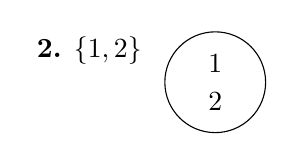
\begin{tikzpicture}[scale=0.8]
			% 2. Set with two elements
			\node at (0,0) {\textbf{2.} \(\{1,2\}\)};
			\draw (2,-0.5) circle (0.8);
			\node at (2,-0.2) {1};
			\node at (2,-0.8) {2};
		\end{tikzpicture}
		\caption*{2. Set with Two Elements}
	\end{minipage}

	\vspace{0.5cm}

	\begin{minipage}{0.45\textwidth}
		\centering
		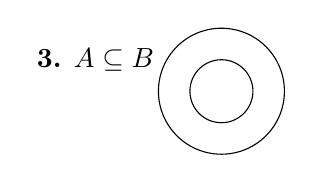
\begin{tikzpicture}[scale=0.8]
			% 3. A subset of B
			\node at (0,0) {\textbf{3.} \(A \subseteq B\)};
			\draw (2,-0.5) circle (1);
			\draw (2,-0.5) circle (0.5);
		\end{tikzpicture}
		\caption*{3. A is a subset of B}
	\end{minipage}
	\hfill
	\begin{minipage}{0.45\textwidth}
		\centering
		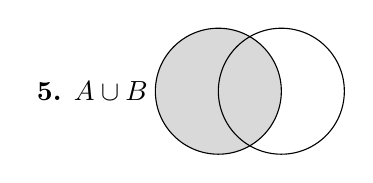
\begin{tikzpicture}[scale=0.8]
			% 5. Union
			\node at (0,0) {\textbf{5.} \(A \cup B\)};
			\begin{scope}
				\clip (2,0) circle(1);
				\fill[gray!30] (3,0) circle(1);
			\end{scope}
			\fill[gray!30] (2,0) circle(1);
			\draw (2,0) circle(1);
			\draw (3,0) circle(1);
		\end{tikzpicture}
		\caption*{5. Union of A and B}
	\end{minipage}

	\vspace{0.5cm}
\end{figure}

\newpage

\begin{figure}
	\centering
	\begin{minipage}{0.45\textwidth}
		\centering
		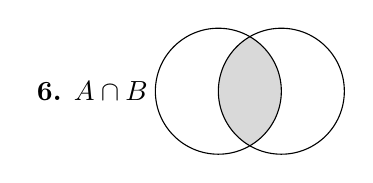
\begin{tikzpicture}[scale=0.8]
			% 6. Intersection
			\node at (0,0) {\textbf{6.} \(A \cap B\)};
			\begin{scope}
				\clip (2,0) circle(1);
				\fill[gray!30] (3,0) circle(1);
			\end{scope}
			\draw (2,0) circle(1);
			\draw (3,0) circle(1);
		\end{tikzpicture}
		\caption*{6. Intersection of A and B}
	\end{minipage}
	\hfill
	\begin{minipage}{0.45\textwidth}
		\centering
		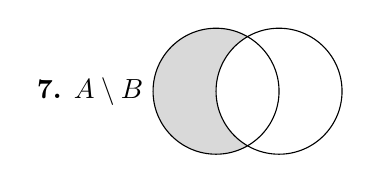
\begin{tikzpicture}[scale=0.8]
			% 7. A \ B
			\node at (0,0) {\textbf{7.} \(A \setminus B\)};
			\fill[gray!30] (2,0) circle(1);
			\begin{scope}
				\clip (3,0) circle(1);
				\fill[white] (2,0) circle(1);
			\end{scope}
			\draw (2,0) circle(1);
			\draw (3,0) circle(1);
		\end{tikzpicture}
		\caption*{7. A minus B}
	\end{minipage}

	\vspace{0.5cm}

	\begin{minipage}{0.45\textwidth}
		\centering
		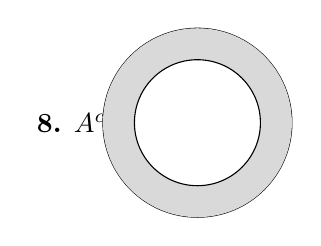
\begin{tikzpicture}[scale=0.8]
			% 8. Complement
			\node at (0,0) {\textbf{8.} \(A^c\)};
			\draw (2,0) circle(1.5);
			\fill[gray!30] (2,0) circle(1.5);
			\fill[white] (2,0) circle(1);
			\draw (2,0) circle(1);
		\end{tikzpicture}
		\caption*{8. Complement of A}
	\end{minipage}
\end{figure}
\smallskip

\subsection{Set Complement Proof}

Given \(A, B \subseteq M\) then \(A \subseteq B \implies B^c \subseteq A^c\)

For some \(x \in B^c\) we know that \(x \notin B\). If \(x \in A\) then \(x \in B\) which is a contradiction. 
Hence \(x \notin A\) therefore, for every \(x \in B^c\) we conclude \(B^c \subseteq A^c\).

\QED


\subsection{Axioms of Set Theory (Zermelo Fraenkel)}

These are Zermelo Fraenkel axioms of set theory including \emph{The Axiom of Choice}.

\begin{enumerate}[label = \Roman*.]
	
	\item \emph{Axiom of Extensionality:} \quad \(\forall A, B: A = B \implies (\forall C: C \in A 
	      \iff C \in B)\)
	
	\item \emph{Empty-Set Axiom:} \quad \(\exists \emptyset : \forall X: X \notin \emptyset\)
	
	\item \emph{Axiom of Pairing:} \quad \(\forall A, B: \exists C: \forall D: D \in C \iff (D = A \lor 
	      D = B)\)	
	
	\item \emph{Axiom of Union:} \quad \(\forall A: \exists B: \forall C: C \in B \iff (\exists D: C 
	      \in D \land D \in A)\)
	
	\item \emph{Axiom of Infinity:} \quad \(\exists N: \emptyset \in N \land (\forall x: x \in N \implies 
	      x \cup \{x\} \in N)\)
	
	\item \emph{Axiom Schema of Specification:} \quad \(\forall A: \exists B: \forall C: C \in B \iff 
	      (C \in A \land P(C))\)
	
	\item \emph{Axiom Schema of Replacement:} \quad \(\forall A: \exists B: \forall y: y \in B \implies 
	      \exists x \in A: y = F(x)\)
	
	\item \emph{Power Set Axiom:} \quad \(\forall A: \exists B: \forall C: C \subseteq A \implies C \in B\)
	
	\item \emph{Foundation Axiom:} \quad \(\forall A \ne \emptyset: \exists B \in A: A \cap B = \emptyset\)
	
	\item \emph{Axiom of Choice:} \quad \(\forall X:
		      \left( \left[ \forall A \in X: A \ne \emptyset \right] \land
		      \left[ \forall B, C \in X: B \ne C \implies B \cap C = \emptyset \right] \right) \\
		      \qquad \implies \exists Y: \forall I \in X: \exists! J \in Y: J \in I\)

			\end{enumerate}

\subsection{The Cartesian Product}

The Cartesian product of two sets \(A\) and \(B\), written \(A \times B\), is the set of 
all ordered pairs in which the first element belongs to \(A\) and the second belongs to \(B\):

\[
	A \times B = \{ (a, b) : a \in A, \land\ b \in B\}
\]

\textbf{Example:}

\begin{table}[H]
	\centering
	\caption{Cartesian Product of \(A = \{1, 2, 3\}\) and \(B = \{4, 5, 6\}\)}
	\begin{tabular}{|c|c|c|c|}
		\hline
		\multirow{3}{*}{\(A \times B\)} & \multicolumn{3}{c|}{\(b \in B\)}                       \\
		\cline{2-4}
		                              & \(4\)                            & \(5\)      & \(6\)      \\
		\hline
		\(a \in A\)                     &                                &          &          \\
		\hline
		\(1\)                           & \((1, 4)\)                       & \((1, 5)\) & \((1, 6)\) \\
		\hline
		\(2\)                           & \((2, 4)\)                       & \((2, 5)\) & \((2, 6)\) \\
		\hline
		\(3\)                           & \((3, 4)\)                       & \((3, 5)\) & \((3, 6)\) \\
		\hline
	\end{tabular}
	\label{tab:cartesian_product}
\end{table}

The general Cartesian product of \(n\) sets can be written as:

\begin{align*}
	X_{i = 1}^{n + 1} A_i & = \left( X_{i = 1}^{n} A_i \right) \times A_{n + 1} \quad \text{with} \quad X_{i = 1}^{1} A_i = A_1 \\
	\text{When } A_i      & = M \ \text{for all } i:                                                                            \\
	M^n                   & := M \times M \times \cdots \times M = X_{i = 1}^{n} M \quad \text{with} \quad M^1 = M
\end{align*}

\subsection{Laws of Set Algebra}

Let \(X\) be the universal set and \(A, B, C \subseteq X\).

\begin{itemize}
	
	\item \(\emptyset \subseteq A\)
	
	\item \(A \subseteq B \iff A \cap B = A \iff A \cup B = B \iff X \setminus B \subseteq X 
		  \setminus A \iff B \subseteq A\)
	
	\item \(A \cup B = B \cup A\) 
	
	\item \(A \cap B = B \cap A\) 
	
	\item \((A \cup B) \cup C = A \cup (B \cup C)\) 
	
	\item \((A \cap B) \cap C = A \cap (B \cap C)\) 
	
	\item \(A \cap (B \cup C) = (A \cap B) \cup (A \cap C)\) 
	
	\item \(A \cup (B \cap C) = (A \cup B) \cap (A \cup C)\) 
		
	\item \(A \cup A = A \quad \text{and} \quad A \cap A = A\)
	
	\item \(A \setminus B = A \cap (X \setminus B) = A \cap \overline{B}\)
	
	\item \(B = \overline{A} \iff (A \cup B = X \land A \cap B = \emptyset)\) 
	
	\item \(\overline{A} \cap \overline{B} = \overline{A \cup B}\) 
	
	\item \(\overline{A} \cup \overline{B} = \overline{A \cap B}\) 
	
	\item \(\overline{\overline{A}} = A\)

\end{itemize}

\subsubsection{Proof of De Morgans's Law for sets and logic}

The complement of \( A \cup B \) is \( \overline{(A \cup B)} \), and the law on disjoint decomposition 
states:

\[
	B = \overline{A} \iff (A \cup B = X) \land (A \cap B = \emptyset)
\]

So define \( \overline{C} := A \cup B \) and \( D := \overline{A} \cap \overline{B} \),
and use Law (11) to show the disjoint decomposition:

\[
	D = C \iff A \cap B = A \cup B
\]

To show:

\[
	D \cup C = X \iff (\overline{A} \cap \overline{B}) \cup (A \cup B) = X
\]

\begin{align*}
	(\overline{A} \cap \overline{B}) \cup (A \cup B)
	 & = (\overline{A} \cup A \cup B) \cap (\overline{B} \cup A \cup B) \quad \text{(Law (8))} \\
	 & = (X \cup B) \cap (X \cup A)                                                            \\
	 & = X \cap X                                                                              \\
	 & = X
\end{align*}

To show:

\[
	D \cap C = \emptyset \iff (\overline{A} \cap \overline{B}) \cap (A \cup B) = \emptyset
\]

\begin{align*}
	(\overline{A} \cap \overline{B}) \cap (A \cup B)
	 & = (A \cap B \cap A) \cup (A \cap B \cap B) \quad \text{(Law (7))}                      \\
	 & = (\overline{A} \cap A \cap \overline{B}) \cup (\overline{A} \cap \overline{B} \cap B) \\
	 & = (\emptyset \cap \overline{B}) \cup (\overline{A} \cap \emptyset)                     \\
	 & = \emptyset \cup \emptyset                                                             \\
	 & = \emptyset
\end{align*}

\QED

\subsection{Indexed Sets}

Let \(X\) be a set, and \( A_i \subseteq X \) for all \( i \in J \), where \emph{J} is the 
\emph{index set}.

If \( J = \{1, 2, \dots, n\} \):

\[
	\bigcup_{i=1}^{n} A_i := A_1 \cup A_2 \cup \dots \cup A_n = \{ x \mid \exists i \in J \ (x \in A_i) \}
\]

\[
	\bigcap_{i=1}^{n} A_i := A_1 \cap A_2 \cap \dots \cap A_n = \{ x \mid \forall i \in J \ (x \in A_i) \}
\]

\[
	X_{i=1}^{n} A_i = \{(a_1, \dots, a_n) \mid a_i \in A_i \}
\]

If \( J \) is any set:

\[
	\bigcup_{i \in J} A_i := \{ x \mid \exists i \in J \ (x \in A_i) \}
\]

\[
	\bigcap_{i \in J} A_i := \{ x \mid \forall i \in J \ (x \in A_i) \}
\]

If \emph{J} is any set, then \( {(A_i)}_{i \in J} \) are pairwise disjoint if and only if:

\[
	\forall i_1, i_2 \in J, \ i_1 \neq i_2 \implies A_{i_1} \cap A_{i_2} = \emptyset
\]

If \emph{J} is any set, then \( {(A_i)}_{i \in J} \) forms a (disjoint) decomposition of \(X\) if 
and only if:

\[
	{(A_i)}_{i \in J} \text{ are pairwise disjoint and } \bigcup_{i \in J} A_i = X
\]

\subsubsection{Partitions Laws}

Let \( A_i, B_j \subseteq X \) for \( i \in I \) and \( j \in J \). Then the following holds:

\begin{itemize}

	\item\emph{De Morgan's Laws:}

	\[
		\overline{\bigcap_{i \in I} A_i}= \bigcup_{i \in I} \overline{A_i} \quad \text{and} \quad 
		\overline{\bigcup_{i \in I} A_i} = \bigcap_{i \in I} \overline{A_i}
	\]

	\item\(
		\bigcap_{i \in I} A_i \cup \bigcap_{j \in J} B_j = \bigcap_{i,j} (A_i \cup B_j) \quad \text{with} 
		\quad \bigcap_{i,j} = \bigcap_{(i,j) \in I \times J}
	\)

	\item\(
		\bigcup_{i \in I} A_i \cap \bigcup_{j \in J} B_j = \bigcup_{i,j} (A_i \cap B_j) \quad \text{with} 
		\quad \bigcup_{i,j} = \bigcup_{(i,j) \in I \times J}
	\)

\end{itemize}

Here, \( I = \{ 1, 2, 3, \dots, n \} \) and \( J = \{ 1, 2, 3, \dots, m \} \). Then:

\begin{align*}
&I \times J = \{ (i, j) \mid 1 \leq i \leq n, 1 \leq j \leq m, i, j \in \Naturals \} \\
&= \{ (1, 1), (1, 2), \dots, (1, m), (2, 1), (2, 2), \dots, (2, m), \dots, (n, 1), (n, 2), \dots, (n, m) \}
\end{align*}

\subsection{Cardinality}

The cardinality of a set is the number of elements in that set.

Let \(A\) and \(B\) be finite sets with \( |A| = n \), \( |B| = m \), and let \(X\) be the finite 
universal set. Then the following holds:

\subsubsection{Cardinality of a Set}

\[
	A = (A \cap B) \cup (A \setminus B), \quad |A| = |A \cap B| + |A \setminus B|
\]

\subsubsection{Cardinality of the complements}

\[
	|A| = |X \setminus A| = |X| - |A|
\]
\[
	A \setminus B = A \cap (X \setminus B), \quad |A \setminus B| = |A| - |A \cap B|
\]

\subsubsection{Cardinality of the Cartesian Product}

\[
	|A \times B| = |A| \cdot |B| = n \cdot m
\]

\subsubsection{Inclusion-Exclusion Formula for Two Disjoint Sets}

\[
	|A \cup B| = |A| + |B| = n + m
\]

\subsubsection{Inclusion-Exclusion Formula for Two Non-Disjoint Sets}

Let \( |A \cap B| = k \), then:

\[
	|A \cup B| = |A| + |B| - |A \cap B| = n + m - k \quad \text{(since we do not count the intersection 
	twice)}
\]

\subsubsection{Inclusion-Exclusion Formula for Three Non-Disjoint Sets}

\begin{align*}
	|A \cup B \cup C| &= |(A \cup B) \cup C| \\ 
	&= |A \cup B| + |C| - |(A \cup B) \cap C| \\
 	&= |A| + |B| - |A \cap B| + |C| - |(A \cap C) \cup (B \cap C)|\\
	&= |A| + |B| + |C| - |A \cap B| - |A \cap C| - |B \cap C| + |A \cap B \cap C|
\end{align*}

\subsubsection{General Formula for the cardinality of the union of sets}

\[
	\left\vert \bigcup_{i = 1}^n M_i \right\vert  = \sum_{I \subseteq \{1, \dots, n\}, I \neq \emptyset}
	{(-1)}^{|I| - 1} \left\vert \bigcap_{i \in I} M_i \right\vert
\]

\subsection{The Power Set}

The Power Set of a set is the set of all subsets of a given set 

\[
	P(x):= \{ M: M \subset X\}
\]

Its cardinality is \(2^n\) with \(n\) being the number of elements in the original set \(X\).

\subsection{Family of Subsets}

Let \(X\) be a non-empty set. A subset \(\mathscr{F}\) of the power set of \(X\) is called a 
set system of \(X\)

\subsection{Partition}

Let \(X\) be a non-empty set. A subset \(\mathscr{F}\) of the power set of \(X\) is called a 
partition if:

\begin{enumerate}
	
	\item \(M \neq  \emptyset\ \forall M \in \mathscr{F}\)
 
	\item \(\bigcap \mathscr{F} = X\)
 
	\item \(M_1 \bigcap M_2 \ne \emptyset \implies M_1 = M_2\ \forall\ M_1, M_2 \in \mathscr{F} \) 

\end{enumerate}

\subsubsection{Properties of Partitions}

\begin{itemize}

	\item Every equivalence relation corresponds to a partition:

		  \[
		      J: \{ R : R\ \text{is an equivalence relation on } X\} \to \{ F: F\ \text{is a partition of } X\}
	      \]

	      where \( J(R) := X / R \) is a bijection.

	\item If \(F\) is a partition of \(X\), then we can define an equivalence relation \( R_F \) by:
	      
		  \[
		      R_F := \{ (x, y) \in X \times X : \exists M \in F\ \text{such that } x, y \in M \}
	      \]
	      
		  Then \( R_F \) is an equivalence relation on \(X\).

\end{itemize}

\subsection{Family of Subsets Operations}

Let \(\mathscr{F}\) be a system of sets (a family of subsets) on the set \(X\). We define:

\[
	\bigcup_{M \in F} M := \bigcup F := \{ x \in X : \text{there exists } M \in F \text{ such that } x 
	\in M \} ,
\]

\[
	\bigcap_{M \in F} M := \bigcap F := \{ x \in X : x \in M \text{ for all } M \in F \} .
\]

\newpage
\section{Relations, Maps and Functions}

\subsection{Map Definition}

A \emph{map} for two sets \(A\) and \(B\) is defined as a subset of \(A \times B\). And it is denoted by 

\[
	f: A \to B \subseteq \{(a, b) \mid (a,b) \in A \times B\}
\]

\subsection{The Set of All Maps}

For the sets \(M\) and \(N\), we define the sets off all maps \(f: M \to N\) as 

\[
	N^M := \{f \mid f: M \to N\}
\]

\subsection{The Characteristic Map}

Given \(T \subseteq M\) we define the \emph{characteristic map} as 

\[
	\mathcal{X}_T: M \to \{0,1\} : m \to \begin{cases} 
		1, &m \in T \\ 
		0, &m \notin T
	\end{cases}
\]

This map tell us if an element is in the subset. Also each map \(\alpha : M \to \{0, 1\}\) defines a 
unique subset \(T\) of \(M\), \(T := M \mid \alpha(m) = 1\).

\subsection{Relations}

A \emph{relation} in mathematics is a connection or relationship between elements of two sets. It's 
formally defined as a subset of the Cartesian product of the sets.

For example, if we have sets \(A\) and \(B\), a relation \emph{R} from \(A\) to \(B\) consists
of ordered pairs \((a,b)\) where \(a \in A\) and \(b \in B\), such that \(a\) is related to \(b\) 
according to some rule or property.

Common types of relations include:

\begin{itemize}

	\item Functions (special relations where each input has exactly one output)

	\item Equivalence relations (reflexive, symmetric, and transitive)

	\item Partial orders (reflexive, antisymmetric, and transitive)

\end{itemize}

Relations can be represented using diagrams, matrices, or sets of
ordered pairs, and they're fundamental to many areas of mathematics including algebra, calculus, and 
discrete mathematics.

\subsection{Types of relations}

Let \(A\) be a set and \(X\) be a relation on \(A\).

\begin{itemize}

	\item \emph{Reflexive:} \(\forall a \in A: (a, a) \in X\) (or written as \(a \sim a\))

	\item \emph{Irreflexive:} \(\forall a \in A: (a, a) \not\in X\)

	\item \emph{Symmetric:} \(\forall a, b \in A: (a, b) \in X \to (b, a) \in X\) (or written as 
		  \((a \sim b) \Rightarrow (b \sim a)\))

	\item \emph{Antisymmetric:} \(\forall a, b \in A: (a, b) \in X \text{ and } (b, a) \in X \to a = b\)

	\item \emph{Transitive:} \(\forall a, b, c \in A: (a, b) \in X \text{ and } (b, c) \in X \to (a, c) 
		  \in X\) (or written as \((a \sim b) \text{ and } (b \sim c) \Rightarrow (a \sim c)\))

	\item \emph{Total:} \(\forall a,b \in A: a \neq b \to (a, b) \in X \text{ or } (b, a) \in X\)

\end{itemize}

\subsection{Equivalence relation}

An \emph{equivalence relation} is a relation that is symmetric, transitive and reflexive.

\textbf{Example:}

\[
	R:= \{ (a,b) \in \Naturals \times \Naturals: a = b\}
\]

\subsection{Functions} 

A subset \( f \subseteq A \times B \) is called a \textbf{function} if:

\[
	(x, y) \in f \text{ and } (x, y') \in f \implies y = y'.
\]

That is, for each \( x \in A \), there exists at most one \( y \in B \) such that \((x, y) \in f.\)

\subsection{The Graph}

\[
	\text{graph}(f):= \{(x, f(x)): x \in X\}
\]

\subsection{The identity}

\[
	\text{id}(f):= idx:= \{(x, x): x \in X\}
\]

\subsection{Image}

The \emph{image (or range)} of a relation \emph{R} from set \(A\) to set \(B\) is the set 
of all elements in \(B\) that are related to at least one element in \(A\). Formally, if 
\(R \subseteq A \times B\) is a relation, then the image of \emph{R} is defined as:

\[
	\img(R) = \{b \in B \mid \exists a \in A \text{ such that } (a,b) \in R\}
\]

In other words, the image consists of all the output values that appear in the ordered pairs of the 
relation. For example, if \(R = \{(1,4), (2,5), (3,4), (2,6)\}\), then \(\img(R) = \{4, 5, 6\}\).

\subsection{Domain}

The \emph{domain} of a relation \emph{R} from set \(A\) to set \(B\) is the set of all elements in 
\(A\) that are related to at least one element in \(B\). Formally, if \(R \subseteq A \times B\) 
is a relation, then the domain of \emph{R} is defined as:

\[
	\text{Dom}(R) = \{a \in A \mid \exists b \in B \text{ such that } (a,b) \in R\}
\]

In other words, the domain consists of all the input values that appear in the ordered pairs of the 
relation. For example, if \(R = \{(1,4), (2,5), (3,4), (2,6)\}\), then \(\text{Dom}(R) = \{1, 2, 3\}\).

\subsection{Equivalence Class}

Let \(\sim\) be an equivalence relation on a set \(A\). For an element \(x \in A\), the 
\emph{equivalence class} of \(x\), denoted by \([x]\), is the set of all elements in \(A\) that are 
equivalent to \(x\). Formally, it is defined as:

\[
	[x] := \{y \in A \mid x \sim y\} \subseteq A
\]

In other words, the equivalence class of \(x\) contains all elements \(y\) in \(A\) such that 
\(x\) is related to \(y\) under the equivalence relation \(\sim\).

\subsection{Quotient Space}

Let \(\sim\) be an equivalence relation on a set \(A\). The \emph{quotient space} of \(A\) by 
\(\sim\), denoted by \(A / \sim\) (or sometimes \(A / R\)), is the set of all distinct equivalence classes of 
elements in \(A\). Formally, it is defined as:

\[
	A/\sim := \{[x] \mid x \in A\}
\]

The quotient space \(A/\sim\) is a partition of the original set \(A\) into disjoint equivalence classes. 
Each element of the quotient space is an equivalence class \([x]\), which itself is a subset of \(A\).

\subsection{Composition of Maps}

The composition of two functions is the operation of applying one function to the result of another 
function. If we have functions \(f: A \to B\) and \(g: B \rightarrow C\), then the composition of \(g\) 
and \(f\), denoted as \(g \circ f\) (read as g composed with f), is a function from \(A\) to \(C\) defined 
by:

\[
	(g \circ f)(a) = g(f(a)) \quad \text{for all } a \in A
\]

The composition applies \(f\) first, then applies \(g\) to the result. 
Note that the co-domain of \(f\) must match the domain of \(g\) for the composition to be defined.

The formal definition is 

\[
	g \circ f := \{ (s, u) \in S \times U \mid \exists t \in T \text{ such that } (s, t) \in f \land (t, u) \in g \}
\]

\textbf{Example:}

Let \(f: \Reals \to \Reals\) be defined by \(f(x) = x^2\) and \(g: \Reals \rightarrow \Reals\) be defined 
by \(g(x) = x+3\). Then:

\[
	(g \circ f)(x) = g(f(x)) = g(x^2) = x^2 + 3
\]

\[
	(f \circ g)(x) = f(g(x)) = f(x+3) = {(x+3)}^2 = x^2 + 6x + 9
\]

Note that \(g \circ f \neq f \circ g\) in general, which shows that function composition is not 
commutative.

\subsection{Types of Functions}

\subsubsection{Injective Functions}

An injective function (also called a one-to-one function) is a 
function that maps distinct elements from the domain to distinct elements in the co-domain.

Formally, a function \(f: A \to B\) is injective if for all \(a_1, a_2 \in A\):

\[
	a_1 \neq a_2 \to f(a_1) \neq f(a_2)
\]

Equivalently, using the contrapositive:

\[
	f(a_1) = f(a_2) \to a_1 = a_2
\]

\subsubsection{Surjective Functions}

A surjective function (also called an onto function) is a function whose image equals its co-domain, 
meaning that every element in the co-domain has at least one pre-image in the domain.

Formally, a function \(f: A \to B\) is surjective if:

\[
	\forall b \in B, \exists a \in A \text{ such that } f(a) = b
\]

\subsubsection{Bijection Functions}

A bijective function (also called a one-to-one correspondence) is a 
function that is both injective and surjective. In other words, every 
element in the co-domain is mapped to by exactly one element in the domain.

Formally, a function \(f: A \to B\) is bijective if it is both:

\begin{itemize}

	\item Injective: \(\forall a_1, a_2 \in A, a_1 \neq a_2 \to f(a_1) \neq f(a_2)\)

	\item Surjective: \(\forall b \in B, \exists a \in A \text{ such that } f(a) = b\)

\end{itemize}

Bijective functions establish a perfect pairing between elements of the domain and co-domain, where each 
element in the domain corresponds to exactly one element in the co-domain, and vice versa. A bijection 
allows us to define an inverse function \(f^{-1}: B \to A\).

\subsection{Propositions on Images and Pre-images under Set Operations}

Let \( f : X \to Y \) be a function.

\subsubsection{Union and Cut Sets}

\begin{itemize}

	\item For subsets \( A_1, A_2 \subseteq X \), we have:

	      \[
		      f(A_1 \cup A_2) = f(A_1) \cup f(A_2)
		      \quad \text{and} \quad
		      f(A_1 \cap A_2) \subseteq f(A_1) \cap f(A_2)
	      \]

	\item For subsets \( B_1, B_2 \subseteq Y \), we have:
	      
	      \[
		      f^{-1}(B_1 \cup B_2) = f^{-1}(B_1) \cup f^{-1}(B_2)
		      \quad \text{and} \quad
		      f^{-1}(B_1 \cap B_2) = f^{-1}(B_1) \cap f^{-1}(B_2)
	      \]
\end{itemize}

\textbf{Proof:}

We prove the second part of 1 and the first part of 2.

Let \( y \in f(A_1 \cap A_2) \). Then there exists \( x \in A_1 \cap A_2 \) such that 
\( f(x) = y \). Since \( x \in A_1 \) and \( x \in A_2 \), it follows that \( y \in f(A_1) \) 
and \( y \in f(A_2) \), hence \( y \in f(A_1) \cap f(A_2) \). Therefore, every element of 
\( f(A_1 \cap A_2) \) is also an element of \( f(A_1) \cap f(A_2) \), so:

\[
	f(A_1 \cap A_2) \subseteq f(A_1) \cap f(A_2)
\]

Let \( x \in f^{-1} (B_1 \cup B_2) \). Then \( f(x) \in B_1 \cup B_2 \), which means \( f(x) \in B_1 \) 
or \( f(x) \in B_2 \). Thus, \( x \in f^{-1}(B_1) \) 
or \( x \in f^{-1}(B_2) \), which implies:
	      
\[
	 x \in f^{-1}(B_1) \cup f^{-1}(B_2)
\]

Hence, both sets contain the same elements and are therefore, equal:
	      
\[
	f^{-1}(B_1 \cup B_2) = f^{-1}(B_1) \cup f^{-1}(B_2)
\]

\QED

\subsubsection{Union and Cut of the whole Domain and Range}

Let \( f : X \to Y \) be a function.

\begin{itemize}

	\item Let \( \mathcal{F} \) be a collection of subsets of \(X\). Then:

   	      \[
		      f\left( \bigcup_{A \in \mathcal{F}} A \right) = \bigcup_{A \in \mathcal{F}} f(A)
		      \quad \text{and} \quad
		      f\left( \bigcap_{A \in \mathcal{F}} A \right) \subseteq \bigcap_{A \in \mathcal{F}} f(A)
	      \]

	\item Let \( \mathcal{G} \) be a collection of subsets of \emph{Y}. Then:

	      \[
		      f^{-1}\left( \bigcup_{B \in \mathcal{G}} B \right) = \bigcup_{B \in \mathcal{G}} f^{-1}(B)
		      \quad \text{and} \quad
		      f^{-1}\left( \bigcap_{B \in \mathcal{G}} B \right) = \bigcap_{B \in \mathcal{G}} f^{-1}(B)
	      \]

\end{itemize}

\textbf{Proof (partial):}

We show the first statement of part (ii); the rest follows analogously.

Let \( x \in f^{-1} \left( \bigcup_{B \in \mathcal{G}} B \right) \). Then:

\[
	f(x) \in \bigcup_{B \in \mathcal{G}} B
	\quad \Leftrightarrow \quad
	\exists B \in \mathcal{G} \text{ such that } f(x) \in B
	\quad \Leftrightarrow \quad
	\exists B \in \mathcal{G} \text{ such that } x \in f^{-1}(B)
\]

Hence:

\[
	x \in \bigcup_{B \in \mathcal{G}} f^{-1}(B)
\]

It follows that:

\[
	f^{-1} \left( \bigcup_{B \in \mathcal{G}} B \right) = \bigcup_{B \in \mathcal{G}} f^{-1}(B)
\]

\QED

\textbf{Example:}

We define \(A = \{1, 0\}\) and \(B = \{2\}\) and \(f(1) = 3\), \(f(2) = 3\) \(f(0) = 1\). Then 

\[
	f(A \cap B) = f( \emptyset) = \emptyset
\]

And 

\[
	f(A) \cap f(B) = 3
\]

\subsection{Even Function}

A real function \(f\) is \emph{even} if

\begin{itemize}
	
	\item \(\forall x \in \text{Dom}(f) \exists -x \in \text{Dom}(f)\)
	
	\item \(\forall x \in \text{Dom}(f) \text{ the following is true } f(x) = f(-x)\)

\end{itemize}

\subsection{Odd Function}

A real function \(f\) is \emph{odd} if

\begin{itemize}
	
	\item \(\forall x \in \text{Dom}(f) \exists -x \in \text{Dom}(f)\)
	
	\item \(\forall x \in \text{Dom}(f) \text{ the following is true } f(x) = - f(x)\)

\end{itemize}

\subsection{Pre-image}

Given \(f: M \to N\). For \(n \in N\) we define 

\[
	f^{-1}(\{n\}) := \{m \in M \mid f(m) = n\}
\]

as the \emph{pre-image} of \(n\). The complete \emph{pre-image} for 
\(T \subseteq N\) is defined as 

\[
	f^{-1}(T) := \bigcup_{t \in T}f^{-1}(\{t\}) = \{m \in M \mid f(m) \in T\}
\]

\subsection{Inverse of a Function}

The \emph{inverse} of a function \(f: A \to B\) is a function \(f^{-1}: B \to A\) that 
reverses the operation of \(f\). That is, if \(f\) maps an element \(a \in A\) to an 
element \(b \in B\), then the inverse function \(f^{-1}\) maps \(b\) back to \(a\).

Formally, a function \(f: A \to B\) has an inverse \(f^{-1}: B \to A\)  
if and only if \(f\) is bijective (both injective and surjective). The inverse function satisfies the 
following properties:

\[
	f^{-1}(f(a)) = a \quad \text{for all } a \in A
\]

\[
	f(f^{-1}(b)) = b \quad \text{for all } b \in B
\]

In other words, composing a function with its inverse yields the identity function. That is:

\[
	f^{-1} \circ f = id_A \quad \text{and} \quad f \circ f^{-1} = id_B
\]

Where \(id_A\) and \(id_B\) are the identity functions on sets \(A\) and \(B\), respectively.

\subsubsection{Steps to Find the Inverse of a Function}

To find the inverse of a function \(f (x)\), follow these steps:

\begin{enumerate}
	
	\item Replace \(f (x)\) with \(y\): \(y = f (x)\)
	
	\item Interchange the variables \(x\) and \(y\): \(x = f (y)\)
	
	\item Solve for \(y\) in terms of \(x\): \(y = f^{-1} (x)\)
	
	\item Verify that the resulting function is indeed the inverse by checking that \(f^{-1}(f(x)) = x\) 
		  and \(f (f^{-1} (x)) = x\)

		\end{enumerate}

\textbf{Example:}

Let's apply the steps above to find the inverse of \(f (x) = 2x + 3\).

\textbf{Step 1: Replace \(f(x)\) with \(y\)}

\[
	y = 2x + 3
\]

\textbf{Step 2: Interchange the variables \(x\) and \(y\)}

\[
	x = 2y + 3
\]

\textbf{Step 3: Solve for \(y\) in terms of \(x\)}

\begin{align*}
	x               & = 2y + 3 \\
	x - 3           & = 2y     \\
	\frac{x - 3}{2} & = y
\end{align*}

So, the inverse function is:

\[
	f^{-1}(x) = \frac{x - 3}{2}
\]

\textbf{Step 4: Verify that \(f^{-1} (f (x)) = x\) and \(f(f^{-1} (x)) = x\)}

Let's verify \(f^{-1} (f (x)) = x\):

\begin{align*}
	f^{-1}(f(x)) & = f^{-1}(2x + 3)         \\
	             & = \frac{(2x + 3) - 3}{2} \\
	             & = \frac{2x}{2}           \\
	             & = x
\end{align*}

And let's verify \(f(f^{-1}(x)) = x\):

\begin{align*}
	f(f^{-1}(x)) & = f\left(\frac{x - 3}{2}\right)     \\
	             & = 2\left(\frac{x - 3}{2}\right) + 3 \\
	             & = (x - 3) + 3                       \\
	             & = x
\end{align*}

Since both compositions yield the identity function, \(f^{-1} (x) = \frac{x - 3}{2}\) is indeed the 
inverse of \(f (x) = 2x + 3\).

\subsubsection{Properties of the Inverse Function}

Let \(f:X\to Y\) be a function.

\begin{itemize}

	\item Assume \(x \sim y \) if \(f(x)= f(y)\) so is \(\sim\) an equivalence relation.

	\item Consider the quotient set \( X_f := X/\sim \), where \( \sim \) is the equivalence relation 
	      defined by \( x \sim x' \iff f(x) = f(x') \). Let \( q_f : X \to X_f \) be the canonical 
		  projection defined by \( q_f(x) = [x] \), and let \( \iota_f : f(X) \to Y \) be the inclusion  
		  map, \( y \mapsto y \). Then the function
	      
		  \[
		      \hat{f} : X_f \to f(X), \quad [x] \mapsto f(x)
	      \]
	  
		  is a bijection, and the original map \(f\) can be written as the composition
	 
		  \[
		      f = \iota_f \circ \hat{f} \circ q_f.
	      \]
	 
		  Here, \( q_f \) is surjective, \( \hat{f} \) is bijective, and \( \iota_f \) is injective. 
		  This yields the following commutative diagram:
	      
		  \begin{center}
				\begin{tikzcd}
					X \arrow[r, "f"] \arrow[d, "q_f"] & Y                         \\
					X_f \arrow[r, "\hat{f}"]          & f(X) \arrow[u, "\iota f"]
				\end{tikzcd}
	      \end{center}

\end{itemize}

\subsection{Transformations of a Function}

Transformations modify the appearance of a function's graph without altering its basic shape.
Here, we examine how different algebraic changes to a function \( f(x) \) affect its graph:

\emph{Vertical Translation:} \( f(x) + a \)
	    
\begin{itemize}
	
	\item Shifts the graph \emph{upward} if \( a > 0 \), and \emph{downward} if \( a < 0 \).
	
	\item Each point on the graph moves vertically by \(a\) units.

\end{itemize}

\emph{Horizontal Translation:} \( f(x + a) \)

\begin{itemize}

	\item Shifts the graph \emph{left} if \( a > 0 \), and \emph{right} if \( a < 0 \).

	\item This is opposite of what might be expected: adding to \(x\) shifts the graph in the negative 
	      direction.

\end{itemize}

\emph{Vertical Scaling (Stretch/Compression):} \( a f(x) \)

\begin{itemize}
	
	\item If \( |a| > 1 \): the graph is \emph{stretched} vertically (taller and narrower).
	
	\item If \( 0 < |a| < 1 \): the graph is \emph{compressed} vertically (shorter and wider).
	
	\item If \( a < 0 \): includes a reflection across the \emph{x-axis}.

\end{itemize}

\emph{Horizontal Scaling (Stretch/Compression):} \( f(a x) \)

\begin{itemize}

	\item If \( |a| > 1 \): the graph is \emph{compressed} horizontally (narrower).

	\item If \( 0 < |a| < 1 \): the graph is \emph{stretched} horizontally (wider).

	\item If \( a < 0 \): includes a reflection across the \emph{y-axis}.

\end{itemize}

\emph{Reflection across the x-axis:} \( -f(x) \)
	
\begin{itemize}

	\item Flips the graph upside-down over the x-axis.

	\item Each point \( (x, y) \) becomes \( (x, -y) \).

\end{itemize}

\emph{Reflection across the y-axis:} \( f(-x) \)

\begin{itemize}

	\item Flips the graph left-to-right over the y-axis.

	\item Each point \( (x, y) \) becomes \( (-x, y) \).

\end{itemize}




\newpage
\section{Mathematical Proofs}

In this section I will provide with some examples of different types of proofs.

\subsection{Proof by Direct Argument}

For any integer \(n\), if \(n\) is even, then \( n^2 \) is even.
We will prove this theorem by direct argument.

Assume \(n\) is an even integer. Then we can write \( n = 2k \) for some integer \(k\).

Now, we compute \( n^2 \):

\[		
	n^2 = {(2k)}^2 = 4k^2 = 2(2k^2)
\]
	
This shows that \( n^2 \) is even, as it can be expressed as \( 2m \) where \( m = 2k^2 \) is an integer.
Therefore, we conclude that if \(n\) is even, then \( n^2 \) is even.

\QED

\subsection{Proof by Contradiction}

If \(n\) is an integer such that \( n^2 \) is even, then \(n\) is even.

We will prove this theorem by contradiction. Assume that \(n\) is an integer such that \( n^2 \) is 
even, but \(n\) is odd. Then we can write \( n = 2k + 1 \) for some integer \(k\).

Now, we compute \( n^2 \):

\[
	n^2 = {(2k + 1)}^2 = 4k^2 + 4k + 1 = 2(2k^2 + 2k) + 1
\]
	
This shows that \( n^2 \) is odd, which contradicts our assumption that \( n^2 \) is even. Therefore, our 
assumption that \(n\) is odd must be false, and thus, \(n\) must be even.

\QED

Another example is the proof that there are infinite prime numbers.

Let us define the prime numbers \(p_1, \dots, p_n\) where we assume \(p_n\) is the biggest prime number. 
If we construct a number 

\[
	q = 1 + p_1 \cdot \cdots \cdot p_n 
\]

This number is bigger than \(p_n\) but it is not divisible by any of the other prime numbers will give us always a residual of 
1. Therefore the assumption that there is a biggest prime number is false.

\QED 

\subsection{Proof by Induction}

For all \( n \in \Naturals \), the sum of the first \(n\) positive integers is given by:

\[
	S(n) = 1 + 2 + 3 + \cdots + n = \frac{n(n+1)}{2}
\]

We will prove this theorem by induction on \(n\).

\textbf{Base Case:} For \( n = 1 \):

\[
	S(1) = 1 = \frac{1(1+1)}{2}
\]

The base case holds.

\textbf{Inductive Step:} Assume that the statement holds for some \( n = k \), i.e., assume that:
	
\[
	S(k) = 1 + 2 + 3 + \cdots + k = \frac{k(k+1)}{2}
\]
	
We need to show that the statement holds for \( n = k + 1 \):

\[
	S(k+1) = S(k) + (k + 1)
\]
	
By the inductive hypothesis, we have:

\begin{align*}
	S(k+1) &= \frac{k(k+1)}{2} + (k + 1) \\
	&= \frac{k(k+1)}{2} + \frac{2(k + 1)}{2}\\
    &= \frac{k(k+1) + 2(k + 1)}{2} \\
	&= \frac{(k + 1)(k + 2)}{2}	
\end{align*}

Thus, the statement holds for \( n = k + 1 \).
By the principle of mathematical induction, the statement holds for all \( n \in \Naturals \).

\QED

\subsection{Proof by Exhaustion}

The only integer solutions to the equation \( x^2 + y^2 = 1 \) are \( (0, 1), (1, 0), (0, -1), (-1, 0) \).

We will prove this theorem by exhaustion. We will check all possible integer values of \(x\) and 
\(y\) such that \( x^2 + y^2 = 1 \).

The possible integer values for \(x\) and \(y\) are \( -1, 0, 1 \). We will check each case:

If \( x = 0 \):

Then \( y^2 = 1 \) gives \( y = 1 \) or \( y = -1 \).

Solutions: \( (0, 1), (0, -1) \).

If \( x = 1 \):

Then \( y^2 = 0 \) gives \( y = 0 \).

Solution: \( (1, 0) \).

If \( x = -1 \):

Then \( y^2 = 0 \) gives \( y = 0 \).

Solution: \( (-1, 0) \).

Thus, the only integer solutions to the equation are:
	
\[
	(0, 1), (1, 0), (0, -1), (-1, 0)
\]

\QED

\subsection{Proof by Cases}

For any integer \(n\), \( n^2 \) is even if and only if \(n\) is even.

We will prove this theorem by cases.

\textbf{Case 1:} Assume \(n\) is even. Then we can write \( n = 2k \) for some integer \(k\).

Now, we compute \( n^2 \):

\[
	n^2 = {(2k)}^2 = 4k^2 = 2(2k^2)
\]

This shows that \( n^2 \) is even.

\textbf{Case 2:} Assume \(n\) is odd. Then we can write \( n = 2k + 1 \) for some integer \(k\).

Now, we compute \( n^2 \):

\[
	n^2 = {(2k + 1)}^2 = 4k^2 + 4k + 1 = 2(2k^2 + 2k) + 1
\]

This shows that \( n^2 \) is odd.

Since both cases have been considered, we conclude that \( n^2 \) is even if and only if \(n\) is even.

\QED

\subsection{Proof by Construction}

There exists an irrational number \(x\) such that \( x^2 \) is rational.

We will construct an irrational number \(x\) such that \( x^2 \) is rational.

Let \( x = \sqrt{2} \). We know that \( \sqrt{2} \) is irrational. Now, we compute \( x^2 \):
	
\[
	x^2 = (\sqrt{2})^2 = 2
\]
	
Since 2 is a rational number, we have constructed an irrational number \( x = \sqrt{2} \) such 
that \( x^2 = 2 \) is rational. Therefore, the theorem is proved.

\QED

\subsection{Proof by Counterexample}

The statement all prime numbers are odd is false.

To prove this theorem, we will provide a counterexample.

The number 2 is a prime number, as its only divisors are 1 and 2. However, 2 is 
even, which contradicts the statement that all prime numbers are odd.

Therefore, the statement All prime numbers are odd is false.
\QED

\subsection{Proof by Contrapositive}

If \(n\) is an integer such that \( n^2 \) is odd, then \(n\) is odd.

We will prove this theorem by contrapositive. The contrapositive of the statement is: If \(n\) is an 
integer such that \(n\) is even, then \( n^2 \) is even.

Assume \(n\) is even. Then we can write \( n = 2k \) for some integer \(k\).

Now, we compute \( n^2 \):
	
\[
	n^2 = {(2k)}^2 = 4k^2 = 2(2k^2)
\]

This shows that \( n^2 \) is even.

Since the contrapositive statement is true, the original statement If \( n^2 \) is odd, then \(n\) is 
odd is also true.

\QED

\subsection{Proof by Reduction to Absurdity}

The square root of 2 is irrational.

We will prove this theorem by reduction to absurdity. Assume that \( \sqrt{2} \) is rational. Then we can 
write:

\[
	\sqrt{2} = \frac{p}{q}
\]

Where \(p\) and \(q\) are integers with no common factors (i.e., the fraction is in the simplest 
form).

Squaring both sides gives:

\[
	2 = \frac{p^2}{q^2}
\]
	
Rearranging gives:

\[
	p^2 = 2q^2
\]
	
This implies that \( p^2 \) is even, and therefore, \(p\) must be even (since the square of an 
odd number is odd). Let \( p = 2k \) for some integer \(k\). Substituting this back into the 
equation gives:

\begin{align*}
{(2k)}^2 &= 2q^2\\	
4k^2 &= 2q^2\\
2k^2 &= q^2
\end{align*}

This implies that \( q^2 \) is even, and therefore, \(q\) must also be even.
Since both \(p\) and \(q\) are even, they have a common factor of 2, which contradicts our 
assumption that \(p\) and \(q\) have no common factors. Therefore, our assumption that 
\( \sqrt{2} \) is rational must be false, and thus, \( \sqrt{2} \) is irrational.

\QED

\subsection{Proof by Analogy}

The set of rational numbers is dense in the set of real numbers.

We will prove this theorem by analogy.

Consider the set of rational numbers \( \Rationals \) and the set of real numbers \( \Reals \). 
The density of \( \Rationals \) in \( \Reals \) means that between any two real numbers, there exists a 
rational number. For example, between the real numbers 1 and 2, we can find the rational 
number \( \frac{3}{2} = 1.5 \). Similarly, between any two real numbers \(a\) and \(b\) (where 
\( a < b \)), we can find a rational number \( r = \frac{a + b}{2} \).

This shows that the set of rational numbers is dense in the set of real numbers.
Therefore, the theorem is proved by analogy.

\QED



\newpage
\section{Order}

\subsection{Principle of the Ordering}

Every non-empty set of natural numbers has a minimum.

\subsection{Order in Fields}

An \emph{ordered field} is a field \(F\) equipped with a total order \( < \) that is compatible with 
the field operations + and \( \cdot \). That is, the order satisfies both algebraic and ordering 
properties.

\subsubsection{Order Axioms for Fields}

A field \(F\) is called an \emph{ordered field} if it satisfies the following properties for all 
\( a, b, c \in F \):

\begin{enumerate}[label=\Roman*.]
    
	\item \emph{Trichotomy:} Exactly one of the following holds:
 
		  \[
 	   			a < b, \quad a = b, \quad a > b
    	   \]

    \item \emph{Transitivity:} If \( a < b \) and \( b < c \), then \( a < c \).

    \item \emph{Additive Compatibility:} If \( a < b \), then \( a + c < b + c \).

    \item \emph{Multiplicative Compatibility:} If \( 0 < a \) and \( 0 < b \), then \( 0 < ab \).

\end{enumerate}

These properties ensure that arithmetic operations respect the order structure.

\subsubsection{Consequences of the Order Axioms}

\begin{itemize}

	\item \( a < b \implies -b < -a \)

	\item \( a < b \land c < 0 \implies ac > bc \)

    \item \(a < 0, b < 0 \implies a + b < 0\) the contrary applies to the multiplication \(ab > 0\)

    \item \(a > 0, b > 0 \implies a + b > 0\)
	
    \item Squares are always non-negative: \( a^2 \ge 0 \)

	\item The order is total: any two elements are comparable

\end{itemize}

\subsubsection{Examples of Ordered Fields}

\begin{itemize}

	\item \( \Rationals \): Rational numbers with the usual order

	\item \( \Reals \): Real numbers with the usual order

	\item \( \Complex \): Complex numbers are not an ordered field, since \( i^2 = -1 < 0 \) 
	      would violate positivity of squares

\end{itemize}


\newpage
\section{The Natural Numbers}

In this section we will take a look at the natural numbers, which are the numbers we use for counting. 
The natural numbers are defined as follows:

We will now define the set of natural numbers, \( \Naturals \), via the following 9 axioms. 
These axioms are known as the \emph{Peano Axioms}. The first 4 axioms define equality on 
the set \( \Naturals \).

\begin{enumerate}[label=\Roman*.]

	\item For every \( x \in \Naturals \), we have \( x = x \).\hfill (Reflexivity)
	
	\item For every \( x, y \in \Naturals \), if \( x = y \) then \( y = x \).\hfill (Symmetry)
	
	\item For every \( x, y, z \in \Naturals \), if \( x = y \) and \( y = z \) then \( x = z \).\hfill 
	      (Transitivity)
	
	\item For all \( x, y \), if \( x \in \Naturals \) and \( x = y \), then \( y \in \Naturals \).\hfill 
	      (Closure of Equality)

\end{enumerate}

The remaining 5 axioms define the structure of \( \Naturals \):

\begin{enumerate}[label=\Roman*.]
	\setcounter{enumi}{4}

	\item \( 1 \in \Naturals \)
	
	\item If \( x \in \Naturals \), then the successor \( S(x) \in \Naturals \).
	
	\item There is no \( x \in \Naturals \) such that \( S(x) = 1 \).
	
	\item For all \( x, y \in \Naturals \), if \( S(x) = S(y) \), then \( x = y \).
	
	\item Let \( P(x) \) be a statement about the natural number \(x\). If:
	
		\begin{itemize}
	
			\item \( P(1) \) is true, and
	
			\item for all \( n \in \Naturals \), if \( P(n) \) is true, then \( P(S(n)) \) is also true,
	
		\end{itemize}
	
		then \( P(x) \) is true for all \( x \in \Naturals \).\hfill (Mathematical Induction)
\end{enumerate}

As shorthand, we denote:

\[
	S(1) = 2, \quad S(S(1)) = 3, \quad S(S(S(1))) = 4, \quad \text{and so on.}
\]

\subsection{Propositions and Proofs}

\subsubsection{Proposition 1: \texorpdfstring{\(n \ne m \implies S(n) \ne S(m)\)}{n!= m implies S (n)!=S (m)}}

\textbf{Proof:} 

We will prove this by contradiction. Assume \( n \ne m \) and \( S(n) = S(m) \). 
By Axiom 8, we have \( n = m \), which is a contradiction. Therefore, \( S(n) \ne S(m) \).

\subsubsection{Proposition 2: \texorpdfstring{\text{For any} \(n \in \Naturals,\ n \ne S(n)\)}{ For any n in N, n!= S (n)}}

\textbf{Proof:} 

\(M = \{n \in \Naturals \| n \ne S(n) \}\ \)

By \(1 \ne S(n)\ \) for any \(n \in \Naturals\), this implies that 1 is part of the set \(M\). 
This implies that \(S(n) \ne S(S(n)) \implies S(n) \in M\ \) By Axiom 9 \(M = \Naturals\)

\subsubsection{Proposition 3: \texorpdfstring{\(n \ne 1\ \exists m \in \Naturals \mid n = S(m)\)}{n!= 1, exists m in N | n = S (m)}}

\textbf{Proof:}

\[
	M = \{1\} \cup\{n \in \Naturals | \text{Proposition 3 is true}\}
\]

We know that 1 ins in the set \(M\). And by proposition 1 we know that

\[
	S(n) = S(S(m)) \implies S(n) \in M
\]

And by Axiom 9 we know that \(M = \Naturals\)

\subsection{Definition of Addition in \texorpdfstring{\(\Naturals\)}{}}

For any pair n, m \(\in \Naturals\) there is a unique way to define

\[
	\text{Add}(n , m) = n + m
\]

\begin{enumerate}
	
	\item \textbf{Base Case:} \(n + 1 = S(n)\)

	\item \textbf{Inductive Step:} \(n + S(m) = S(n + m) \iff S(n + m)\)

\end{enumerate}

\textbf{Uniqueness:} 

Suppose: \textit{A} \& \textit{B} satisfy our conditions. Fix n and then let \(M = \{ m \in \Naturals | 
A(n,m) = B(n, m)\}\). Then

\[
	A(n,1) = S(n) = B(n,1) \implies 1 \in M
\]

\[
	m \in M \implies A(n, m) = B(n, m) \implies A(n, S(m)) = S(A(n, m)) = S(B(n, m)) = B(n, S(m))
\]

\[
	\implies A(n , S(m)) = B(n, S(m))
\]

by Axiom 9 we know that \(M = \Naturals\) and A = B

\textbf{Construction:} For \(n = 1\) Define \(A(n, m) = S(m)\)

\begin{enumerate}
	
	\item \(A(n, 1) = S(n) = S(1)\)
	
	\item \(A(n, S(m)) = S(A(n, m)) = S(S(m))\)

\end{enumerate}

Define: \(A(S(n), S(m)) = S(A(n, m))\)

\begin{enumerate}

	\item \(A(S(n), 1) = S(A(n, 1)) = S(S(n))\)

	\item \(A(S(n), S(m)) = S(A(n, m)) = S(S(m))\)

\end{enumerate}

\textbf{Commutativity of Addition:}

The proposition says \(n + m = m + n\) for any \(n, m \in \Naturals\). We will prove this by 
induction on \(m\). Fix n and consider \(M = \{ n \in \Naturals | A(n, m) = A(n, m)\}\)

Now recall that \(A(n, 1) = S(n)\)

For \(n = 1\):

\[
	A(n, 1) = S(1) = A(1, n) \implies 1 \in \Naturals
\]

also \(A(n , k) = 1 + k \implies 1 + m = S(m) \implies 1 + m = m + 1 \implies 1 \in \Naturals\)

Suppose: \(n \in \Naturals \implies n + m = m + n\) or \(A(n, m) = A(m, n)\)

By construction \(A(S(n), m) = S(A(n, m))\) and by definition
\(A(S(n), m) = S(A(n, m)) = A(m, S(n)) = S(n) + m =  m + S(n) \implies S(n) \in M \implies 
\text{by induction } M = \Naturals\).

\newpage
\section{The Archimedean Principle}

For any real number \( x \in \Reals \), there exists a natural number \( n \in \Naturals \) such 
that \( n > x \).

In other words, no matter how large a real number you choose, there is always a natural number that 
is larger. Similarly, for any positive real number \( \epsilon > 0 \), there exists a natural number 
\( n \in \Naturals \) such that \( \frac{1}{n} < \epsilon \).

\textbf{Proof:}

We prove the Archimedean Principle by contradiction.

Assume that there exists some real number \( x \in \Reals \) such that \( n \leq x \) for all 
\( n \in \Naturals \). That is, \(x\) is an upper bound for the set \( \Naturals \subset \Reals\), baked up 
by the Completeness Axiom of the real numbers.

Let \( S = \sup(\Naturals) \), the least upper bound of \( \Naturals \). Then 
\( S - 1 < \sup(\Naturals) \), so \( S - 1 \) is not an upper bound of \( \Naturals \). Hence, 
there exists \( n_0 \in \Naturals \) such that:

\[
	n_0 > S - 1 \Rightarrow n_0 + 1 > S
\]

But \( n_0 + 1 \in \Naturals \), which contradicts the assumption that \emph{S} is an upper bound of 
\(\Naturals \). Therefore, our assumption must be false, and the theorem is proven.

\QED

\subsection{Equivalent Formulations}

The Archimedean Principle is often stated in different but equivalent ways:

\begin{itemize}
	
	\item For any \( \epsilon > 0 \), there exists \( n \in \Naturals \) such that \( \frac{1}{n} < 
		  \epsilon \).
	
	\item For any \( a, b \in \Reals \) with \( a > 0 \), there exists \( n \in \Naturals \) such that 
	      \( na > b \).

\end{itemize}

\subsection{Applications}

\begin{enumerate}
	
	\item \textbf{Density of Rational Numbers:} The Archimedean Principle helps in proving that between 
		   any two real numbers, there exists a rational number.

	\item \textbf{Limits and Infinitesimals:} It ensures that sequences like 
	      \( \left\{ \frac{1}{n} \right\}\) converge to 0, foundational in real analysis and calculus.

	\item \textbf{Bounding Functions:} It is used in analysis to show that functions do not grow faster 
	      than natural numbers in certain contexts.

	\item \textbf{Non-Existence of Infinitely Small Numbers:} The principle implies that real numbers do 
	      not contain infinitesimals (nonzero numbers smaller than all \( \frac{1}{n} \)), distinguishing 
		  \( \Reals \) from non-standard number systems.

\end{enumerate}


\newpage
\section{Arithmetic}

\subsection{Even and Odd numbers}

A natural number \(a\) is \emph{even} if \(a = 2k\) with \(k \in \Naturals\).

A natural number \(b\) is \emph{odd} if \(b = 2q - 1\) with \(q \in \Naturals\).

\subsection{Perfect Squares}

A natural number \(a\) has a \emph{perfect square} if \(\sqrt{a} \in \Naturals\).

\subsection{Division Algorithm}

Given any two integers \(a\) and \(b\) with \(a > 0\), there exists unique integers \(q\) and \(r\) such that 
\(b  =qa + r\) with \(0 \ge r < a\).

\textbf{Proof:}

Let \(S = \{b - xa \mid b - xa \ge 0, x \in \Integers\}\)

By the well ordering principle of the natural numbers we know that our set has 
minimum \(r\). 

First we prove \( 0 \le r\)

If \(b \ge 0\) then let \(x = 0 \implies b \in S\).
For \(b < 0\) then let \(x = b\). Thus 

\[
	b - ba  = b(1 - a) \implies b - ba \in S
\]

Now to prove that \(r < a\), assume \( r \ge a\), but then 


\begin{align*}
	b  - qa &\ge a \\
	b  - qa - a &\ge 0\\ 
	b  - a(q + 1) &\ge 0\\ 
	b  - a(q + 1) &\ge 0 \implies b - a(q + 1) \in S\\ 
\end{align*}

And \(b - a(q + 1) < b - aq = r \implies r < a\) therefore, we have a contradiction.

Now we will prove the uniqueness. 

Assume \(pq + r = a = pq' + r'\) with \(q \ne q' \) and \(r \ne r'\)

\[	
	r - r' = a(q - q') = 0
\]

Using the property of inverses of \(\Integers \setminus \{0\}\) as a Field we know that 
\(r = r'\) and \(q - q'\).

\QED 

\subsection{Prime Numbers}

A \emph{prime number} \(p \in \Naturals \setminus \{1\}\) fulfills the following condition:

\begin{enumerate}[label= \Roman*.]
	\item \(p\) is only divisible by itself and 1.
\end{enumerate}

\subsection{Pythagorean Triplets}

\emph{Pythagorean triplets} are 3 natural numbers such that 

\[
	a^2 + b^2 = c^c
\]

\subsection{Divisibility}

A number \(a \in \Integers\) is divisible a number \(b \in \Integers\) if 

\[
	a = kb \quad k \in \Integers
\]

\subsection{Division}

Given \(a,b \in \Integers\). There exists unique \(q,r \in \Integers\) such that 

\[
	a = qb + r \quad 0 \le r < |b|
\]

\subsection{Greatest Common Denominator}

For two integers \(a, b \in \Integers\) with \((a,b) \neq (0,0)\), the positive
integer \(t\) satisfying

\begin{itemize}

	\item \(t \mid a\) and \(t \mid b\),

	\item for all \(c \in \Integers\) with \(c \mid a\) and \(c \mid b\), it follows that \(c \mid t\),

\end{itemize}

is called the \emph{greatest common divisor} (gcd) of \(a\) and \(b\) denoted as \(t = \gcd(a,b)\).

If \(t = 1\), then \(a\) and \(b\) are said to be \emph{coprime} or \emph{relatively prime}.

\subsection{The Euclidean Algorithm}

If \(a = bq + r\) then \(\gcd(a, b) = \gcd(b, r)\). 

\textbf{Input:} \(a, b \in \mathbb{Z}\), \(a \neq 0 \neq b\).  
\textbf{Output:} The greatest common divisor \(t\) of \(a\) and \(b\).

\textbf{Algorithm:}

\begin{enumerate}

	\item If \(a = 0\), then return \(|b|\). If \(b = 0\), return \(|a|\).

	\item Set \(r_1 := a\); \(r_2 := b\); \(k := 2\).

	\item As long as \(r_k \neq 0\), define \(r_{k+1} := r_{k-1} \bmod r_k\).

	\item As soon as \(r_k = 0\), return \(r_{k-1}\).

\end{enumerate}

In simpler terms, as long the remainder is not zero, we keep dividing the previous remainder by the current
remainder and updating the remainders. When we reach a remainder of zero, the previous remainder is the gcd. 

\textbf{Proof:}

Notice, that the algorithm terminates because the sequence given \(r_n\) is monotone decreasing due to \(0 \le r < b\) and 
the well ordering principle of the natural numbers.

For the correctness: given is \(a = bq + r\) to show that \(\gcd(a, b) = \gcd(b, r)\). This is like saying 

\begin{align*}
	\gcd(a,b) & = gcd(b, r) \\ 
	\gcd(b,r) & = \gcd(r, r_1)\\
	\gcd(r, r_1) & = \gcd(r_1, r_2) \\
	& \vdots \\
	\gcd(r_{n-1}, r_{n}) & = \gcd(r_n, 0) = r_n 
\end{align*}

Let \(d\) be a common divisor of \(a\), \(b\). Then \(d \mid a\) and \(d \mid b\), so \(d \mid ((a - bq) = r) \implies d \mid r \).

Let \(e\) be a common divisor of \(b\), \(r\). Then \(e \mid b\) and \(e \mid r\), so \(e \mid ((bq + r) = a) \implies e \mid a \).

Thus, the set of common divisors of \(a\), \(b\) is the same as the set of common divisors of \(b\), \(r\),
so their greatest common divisors are equal.

\QED 

\textbf{Example:}

Find \(\gcd(252, 198)\):

\begin{align*}
	r_{n - 1} & = q_{n - 1} r_n + r_{n + 1} \\
	252 & = 1 \cdot 198 + 54  \\
	198 & = 3 \cdot 54 + 36   \\
	54  & = 1 \cdot 36 + 18   \\
	36  & = 2 \cdot 18 + 0
\end{align*}

So, \(\gcd(252, 198) = 18\). 

\subsection{Euclidean Algorithm as Linear Map}

Given \(E := \{(a,b)^T \mid a, b \in \Integers, b \ne 0 \}\) and 

\[
	\varepsilon: E \to \Integers^{2 \times 1} : 
	\begin{bmatrix}
		a \\ 
		b
	\end{bmatrix}
	\mapsto
	\begin{bmatrix}
		b \\
		a \mod b
	\end{bmatrix}
\]

Then the Euclidean algorithm can be described as repeated application of \(\varepsilon\) until the second
component is zero. The first component at that point is the gcd.

\[
	\varepsilon^{k - 1}
	\begin{bmatrix}
		a \\ 
		b
	\end{bmatrix}
	= \varepsilon \circ \cdots \circ \varepsilon
	\begin{bmatrix}
		t \\ 
		0
	\end{bmatrix}
\]

\(t = \gcd(a,b)\).

Also, we can express \(\varepsilon\) as a matrix multiplication:

\[
	\varepsilon
	\begin{bmatrix}
		a \\ 
		b
	\end{bmatrix}
	=
	\begin{bmatrix}
		0 & 1 \\
		1 & -q
	\end{bmatrix}
	\begin{bmatrix}
		a \\ 
		b
	\end{bmatrix}
	= 
	\begin{bmatrix}
		b \\ 
		r
	\end{bmatrix}
\]

with \(a = qb + r\) and \(q \in \Integers, 0 \le q < |b|\).

\subsection{Bezout Identity}

This is one of the most important properties of the \emph{gcd}. 
Given \(a, b \in \Integers\), not both zero, there exist integers \(\alpha, \beta \in \Integers\) such that

\[
	\gcd(a, b) = a\alpha + b\beta
\]

This equation comes directly from \emph{Euclid's Algorithm}. For the intuition, when writing your iterations 
you can manipulate them to arrive at the solution.

\textbf{Proof:}

Given 

\[
	M := \{a\alpha + b \beta \mid a\alpha + b \beta > 0 \land \alpha \in \Integers \land \beta \in \Integers\}
\]

\(M\) is not empty because of \(\alpha, \beta \in M\), and it has a minimum by the well ordering principle 
of the natural numbers which we will call \(c\).

Then, let \(k \in M\). Then there exist \(q \in \Naturals_0\) and \(r \in \Naturals_0\) with \(r < c\) such 
that

\[
	k = qc + r
\]

because \(k\) and \(c\) are elements of \(M\) we should be able to find \(r_1, r_2, s_1, s_2\)  such that 

\[
	k = r_1 a + s_1 b \quad c = r_2 a + s_2 b
\]

Now let us

\begin{align*}	
	k = r_1 a + s_1 b &= qc + r \\ 
		r_1 a + s_1 b &= q(r_2 a + s_2 b) + r \\ 
		r &= r_1 a + s_1 b - q(r_2 a + s_2 b)  \\ 
		r &= r_1 a + s_1 b - qr_2 a  -qs_2 b  \\
		r &= (r_1  - qr_2)a + (s_1   -qs_2) b 
\end{align*}

\(r \ge 0\) and  \(r < c\), but if \(r \ne 0\) then \(r \in M\) would be the minimum which is a contradiction to the assumption 
that \(c\) is the minimum, also \(r = 0\), \(k = qc\). Thus, \emph{every element of M is multiplicity of c}. Therefore, 
\(a,b\) are also divisible by \(c\).

Now we need to show that \(c\) is in fact the greatest common divisor. \(c = r_2 a + s_2 b\) 

\[
	c = a \alpha_0 + b \beta_0
\]

Because \(c \mid a \land c \mid b\) we know that \(c \mid a \alpha_0 + b \beta_0 \). We also 
know that \(c \mid \gcd(a,b)\) and thus, \(|c| =|g = \gcd(a,b| \) but because both are positive \(c = g\).

\QED

\subsection{Euclidean Algorithm as Matrix Multiplication}

\textbf{Input:} \(a, b \in \mathbb{Z}\), \(a \neq 0 \neq b\).  

\textbf{Output:} \(t = \gcd(a,b)\) and \(\alpha, \beta \in \mathbb{Z}\) with 
\(\alpha a + \beta b = t\).

\textbf{Algorithm:}

\begin{enumerate}

	\item If \(a = 0\), return \(|b|\), \(\alpha = 0\), and 
    \(\beta = b / |b|\).  
    If \(b = 0\), return \(|a|\), \(\alpha = a / |a|\), and \(\beta = 0\).
    
    \item Compute, for \(r_1 := a\) and \(r_2 := b\), the sequence 
    \((r_n)\) using Algorithm~5.18, i.e.  
    \(r_{n-1} = q_{n-1} r_n + r_{n+1}\) with \(q_{n-1} \in \mathbb{Z}\) 
    and \(r_k = 0\).
    
    \item Define 
    
	\[
		A_n := 
		\begin{bmatrix}
			0 & 1 \\
			1 & -q_{n-1}
		\end{bmatrix}	
	\]

	for \(1 \le n \le k - 2\). Then the first row of the matrix \(A_{k - 2} \cdots A_1\) returns the pair \(\alpha. \beta\)
\end{enumerate}

\subsection{Prime Field}

Given \(p \in \Naturals, p > 1\) is prime, then \(\Integers / p \Integers\) is a field with \(p\) elements. It can also 
be noted \(\Field_p\)

\textbf{Proof:} 

We need to show that for \(a + p \Integers \ne p \Integers\) there exists some \(b + p \Integers\) such that \((a + p\Integers))(b + p\Integers) = 1 + p\Integers\).

For \(a \notin p \Integers\) we know that \(gcd(a,p) = 1\) thus, we do not have zero divisors.

\subsection{Implication of Prime Numbers}

For \(a, b \in \Integers\) and a prime number \(p\)

\[
	p \mid ab \implies (p \mid a ) \lor (p \mid b)
\]

\textbf{Proof:} 

``\(\Rightarrow\)'' Let \(p\) be a prime and \(a,b \in \Integers\)
with \(p \mid ab\). Assume \(p \nmid a\). Then there exist \(\alpha,\beta \in \Integers\)
with \(\alpha p + \beta a = 1\). Since \(p \mid ab\), it follows that
\(p \mid \alpha p b + \beta ab = (\alpha p + \beta a)b = b\).

``\(\Leftarrow\)'' Let \(c \in \Naturals\) be a divisor of \(p\). Then there exists
\(d \in \Naturals\) with \(p = cd\). In particular \(1 \le c \le p\) and
\(1 \le d \le p\) and \(p \mid cd\). By our assumption it follows that
\(p \mid c\) or \(p \mid d\), i.e. \(p \le c\) or \(p \le d\). Together with
\(c \le p\) and \(d \le p\) this forces \(c = 1\) or \(c = p\). Hence, \(p\)
has no nontrivial divisors and is prime.

\QED

\subsection{Fundamental Theorem of Arithmetic}

Every integer greater than 1 can be written in the form

\[
	p_1^{n_1}p_2^{n_2} \cdots p_k^{n_k}
\]

Where \(n_i \geq 0\) and the \(p_i\) are distinct primes. The factorization is unique, except possibly for 
the order of the factors.

\textbf{Example.}

\[
	4312 = 2 \cdot 2156 = 2 \cdot 2 \cdot 1078 = 2 \cdot 2 \cdot 2 \cdot 539 = 2 \cdot 2 \cdot 2 \cdot 7 
	\cdot 77 = 2 \cdot 2 \cdot 2 \cdot 7 \cdot 7 \cdot 11
\]

That is,

\[
	4312 = 2^3 \cdot 7^2 \cdot 11
\]

Approach to the proof: 

\begin{itemize}

	\item The Fundamental Theorem of Arithmetic says that every integer greater than 1 can be factored 
		 uniquely into a product of primes.
	
	\item Euclid’s lemma says that if a prime divides a product of two numbers, it must divide at least 
		  one of the numbers.
	
	\item The least common multiple \([a, b]\) of nonzero integers \(a\) and \(b\) is the smallest positive 
	      integer divisible by both \(a\) and \(b\).

\end{itemize}


\subsection{Lemmas}

\textbf{Lemma} 

If \(m \mid pq\) and \(\gcd(m, p) = 1\), then \(m \mid q\).

\textbf{Proof:} 

Write \(1 = \gcd(m, p) = am + bp\) for some \(a, b \in \Integers\). Then

\[
	q = amq + bpq
\]

Since \(m \mid amq\) and \(m \mid bpq\) (because \(m \mid pq\)), we conclude \(m \mid q\).

\QED

\textbf{Lemma} 

If \(p\) is prime and \(p \mid a_1a_2 \cdots a_n\), then \(p \mid a_i\) for some \(i\).

\textbf{Proof (Case \(n=2\)):} 

Suppose \(p \mid a_1a_2\), and \(p \nmid a_1\).
Then \(\gcd(p, a_1) = 1\), and by the previous lemma, \(p \mid a_2\).

For general \(n > 2\): Assume the result is true for \(n-1\). Suppose \(p \mid a_1a_2 \cdots a_n\).
Group as \((a_1a_2 \cdots a_{n-1})a_n\).

By the \(n=2\) case, either \(p \mid a_n\) or \(p \mid a_1a_2 \cdots a_{n-1}\), and by induction, 
\(p \mid a_i\) for some \(i\).

\QED

\subsection{Proof of the Fundamental Theorem of Arithmetic}

\textbf{Existence:}

Use induction on \(n > 1\)Let \(X = (X_{1}, \ldots, X_{n})^{T} : \Omega \to X\) be a random variable with
statistical model \(P = \{ P^{n}_{\theta} : \theta \in \Theta \}\).
Furthermore, let \(x_{1}, \ldots, x_{n}\) be a sample and let \(\alpha \in [0,1]\).

A mapping \(I\) that assigns to each sample
\(x = (x_{1}, \ldots, x_{n})^{T} \in X\) a subset \(I(x) \subset \Theta\)
is called a \((1 - \alpha)\)-confidence region for \(\theta\) if

\[
    \Prob_{\theta}\bigl( \theta \in I(X_{1}, \ldots, X_{n}) \bigr)
    \ge 1 - \alpha
\]

for all \(\theta \in \Theta\).

If \(\Theta \subset \Reals\) and \(I(x)\) is an interval for all \(x \in X\),
then \(I\) is called a \((1 - \alpha)\)-confidence interval.

Base case: \(n = 2\) is prime.

Inductive step: If \(n\) is prime, done. Otherwise, \(n = ab\), with \(1 < a, b < n\).
By induction, both \(a\) and \(b\) factor into primes, so \(n\) does too.

\textbf{Uniqueness:}

Suppose:

\[
	p_1^{m_1} \cdots p_j^{m_j} = q_1^{n_1} \cdots q_k^{n_k}
\]

With all \(p_i\) and \(q_i\) distinct primes.

Since \(p_1\) divides the LHS, it divides the RHS. So \(p_1 \mid q_i^{n_i}\) for some \(i\), hence 
\(p_1 = q_i\). Re-order so \(p_1 = q_1\). Then:

If \(m_1 > n_1\), divide both sides by \(q_1^{n_1}\):

\[
	p_1^{m_1-n_1} \cdots p_j^{m_j} = q_2^{n_2} \cdots q_k^{n_k}
\]

But then \(p_1\) divides LHS but not RHS, contradiction. So \(m_1 = n_1\). Cancel and repeat.

Eventually, all \(p_i\) match with some \(q_i\), and the exponents are equal. So the factorizations
are the same up to order.

\QED

\subsection{Least Common Multiple}

The least common multiple of \(a\) and \(b\), denoted \([a, b]\), is the smallest positive integer 
divisible by both.

\textbf{Example:}

\[
	[6, 4] = 12, \quad [33, 15] = 165
\]

\subsection{Multiplication Property of the Least Common Multiple}

\[
	[a, b] \cdot \gcd(a, b) = ab
\]

\textbf{Proof:}

Let:

\[
	a = p_1 \cdots p_lq_1 \cdots q_m, \quad b = q_1 \cdots q_mr_1 \cdots r_n
\]

Then:

\begin{align*}
	\gcd(a, b) & = q_1 \cdots q_m                                 \\
	[a, b]     & = p_1 \cdots p_lq_1 \cdots q_mr_1 \cdots r_n     \\
	ab         & = p_1 \cdots p_lq_1^2 \cdots q_m^2r_1 \cdots r_n
\end{align*}

So:

\[
	[a, b] \cdot \gcd(a, b) = ab
\]

\textbf{Example:}

\[
	\gcd(36, 90) = 18, \quad [36, 90] = 180, \quad 36 \cdot 90 = 32400 = 18 \cdot 180
\]


\subsection{Second Proof of the Fundamental Theorem of Arithmetic}

Given \(n \in \Naturals\) has \(1\) as a prime factor. Suppose that every natural number 
smaller than \(n\) can be factorized into primes. 

If \(n\) is a prime number then it is itself its prime factorization. Else. there 
are \(b, c \in \Integers\) with \(n = bc\) \(1 < b, c<n\). By our induction's supposition, 
\(b\) and \(c\) have also a prime factorization.

\[
	b = p_1 \cdot p_2 \cdots p_r \text{ and } c = q_1 \cdot q_2 \cdots q_s
\]

with \(p_i, p_j\) \(1 \le \le r\) and \(1 \le j \le s\) prime numbers. The product is 
the prime factorization of the \(n\).

The uniqueness is given by \emph{the implication of prime numbers}.

\QED

\subsection{Goldbach's Conjecture}

Every even integer greater than 4 can be written as the sum two primes.

\subsection{Prime Factorization}

To find the \emph{prime factorization} of a number \(a\) the algorithm goes as follows 

\begin{itemize}

	\item Let \(n\) be the first prime number. 

	\item  Try dividing \(a\) by \(n\). If \(n \mid a\) note the number and set \(a = a \div n\) to repeat this step. If \(n\) 
	did not divide \(a\) set \(n\) to the next prime number and repeat this step. 

	\item When 1 was reached using the previous step then the algorithm terminates and the noted numbers is our prime factorization 
	of \(a\).

\end{itemize}

\subsection{GCD via Prime factorization}

The \(\gcd\) of two or more number can also be found with the following algorithm.

\begin{itemize}
	
	\item Find the prime factorization of all target numbers.

	\item Note the number which appear in both prime factorization always taking the one with least exponent.
	
	\item Multiply the noted prime factors together. 
	
\end{itemize}


\newpage
\section{Real Numbers}

A way of defining the \emph{real numbers} is via the \emph{Cauchy sequences}. Another way is via 
the axioms of a field. 

\subsection{Definition as Cauchy Sequences}
 
Let \( K \) be an ordered field. On the set
		
\[
	\operatorname{ch}(K) := \{ x : \Naturals \to K \mid x \text{ is a Cauchy sequence} \}
\]
		
and on the set
	
\[
	c(K) := \{ x : \Naturals \to K \mid x \text{ is a convergent sequence} \}
\]

we can define an addition and a multiplication as follows:

If \( x = {(x_n)}_{n \in \Naturals} \) and \( y = {(y_n)}_{n \in \Naturals} \) are Cauchy sequences 
(respectively, convergent sequences), then their sum is defined as
	
\[
	x + y := {(x_n)}_{n \in \Naturals} + {(y_n)}_{n \in \Naturals} := {(x_n + y_n)}_{n \in \Naturals}
\]
	
and their product is defined as

\[
	x \cdot y := {(x_n)}_{n \in \Naturals} \cdot {(y_n)}_{n \in \Naturals} := {(x_n \cdot y_n)}_{n \in 
	\Naturals}
\]

The sum and product satisfy all field axioms except for the existence of the multiplicative inverse.
The zero element is \( 0_{\Naturals} = (0, 0, \ldots) \), the unit element is \( 1_{\Naturals} = (1, 1, 
\ldots) \), and the additive inverse of \( x = {(x_n)}_{n \in \Naturals} \) is 
\( -x = {(-x_n)}_{n \in \Naturals} \). We demonstrate the distributive law as an example:

Let \( x = {(x_n)}_{n \in \Naturals}, y = {(y_n)}_{n \in \Naturals}, z = {(z_n)}_{n \in \Naturals} \) be 
Cauchy sequences (convergent sequences). Then we have:

\begin{align*}
	x(y + z) &= {(x_n)}_{n \in \Naturals} \cdot \left( {(y_n)}_{n \in \Naturals} + {(z_n)}_{n \in \Naturals} \right)\\
	&= {(x_n)}_{n \in \Naturals} \cdot {(y_n + z_n)}_{n \in \Naturals}\\ 
	&= {(x_n (y_n + z_n))}_{n \in \Naturals}\\
	&= {(x_n y_n + x_n z_n)}_{n \in \Naturals}\\
	&= {(x_n y_n)}_{n \in \Naturals} + {(x_n z_n)}_{n \in \Naturals}\\
	&= xy + xz.
\end{align*}

We now aim to construct the ordered field \( \Reals \) of the real numbers;
it will have the following properties:

\begin{itemize}
	
	\item There exists an injective mapping \( j : \Rationals \to \Reals \) which respects addition, 
    	  multiplication, and order, such that the following holds:
		
		For all \( z, w \in \Reals \) with \( z < w \), there exists an \( x \in \Rationals \) such that
		
		\[
			z < j(x) < w
		\]

	\item Every Cauchy sequence in \( \Reals \) converges.

\end{itemize}

Via \(j\), we identify \( \Rationals \) with \( j(\Rationals) \) and consider \( \Rationals \) as a 
subset of \( \Reals \). In \( \Reals \), the following will additionally hold:

\begin{itemize}

	\item For all \( y > 0 \) and \( n \in \Naturals \), the equation \( x^n = y \) has a solution.

	\item Every bounded above subset of \( \Reals \) has a supremum.

\end{itemize}

We define the following relation on the set \( \operatorname{ch}(\Rationals) \) of all Cauchy sequences 
in \( \Rationals \):

\[
	x \sim y \quad \text{if and only if} \quad x - y \text{ is a null sequence}
\]

That is, \( {(x_n)}_{n \in \Naturals} \sim {(y_n)}_{n \in \Naturals} \) if and only if

\[
	x_n - y_n \to 0 \quad (n \to \infty)
\]

\subsection{Definition}

The set

\[
	\Reals := \{ {[x]}_{\sim} : x \in \operatorname{ch}(\Rationals) \}
\]

is called the set of real numbers.

Analogous to the construction of the rational numbers, the real numbers consist of equivalence classes.
Roughly speaking, an equivalence class consists of those Cauchy sequences in \( \Rationals \) that exhibit 
the same limit behavior.

Equipped with the addition

\[
	+ : \Reals \times \Reals \to \Reals, \quad [x], [y] \mapsto [x] + [y] := [x + y]
\]

and the multiplication

\[
	\cdot : \Reals \times \Reals \to \Reals, \quad [x], [y] \mapsto [x] \cdot [y] := [xy]
\]

\( \Reals \) is a field. The zero element is \( [0_{\Naturals}] \), and the unit element is 
\( [1_{\Naturals}] \).


\input{src/Numbers/Complex.tex}

\newpage
\section{Topology}

In this section, we introduce essential vocabulary used in topology. Each term is accompanied by a 
brief explanation and its formal mathematical definition.

\subsection{Introduction to topological nomenclature}

\subsubsection{Open Ball} (\( B_\varepsilon(x) \)) 

For a metric space \( (X, d) \), the \emph{open ball} centered at 
\( x \in X \) with radius \( \varepsilon > 0 \) is defined as: 
	      
\[
	B_\varepsilon(x) := \{ y \in X \mid d(x, y) < \varepsilon \}
\]

It represents the set of all points within distance \( \varepsilon \) from \(x\), excluding the boundary.

\subsubsection{Open Set}
	     
A subset \( U \subseteq X \) of a topological space is called 
\emph{open} if for every point \( x \in U \), there exists an \( \varepsilon > 0 \) 
such that the open ball \( B_\varepsilon(x) \subseteq U \). 
Intuitively, an open set contains none of its boundary points and every point has some 
wiggle room around it.

\subsubsection{Closed Set} 
	      
A subset \( A \subseteq X \) is called \emph{closed} if its 
complement \( X \setminus A \) is open. Equivalently, \(A\) contains all its limit points. 
That is, \(A\) is closed if it includes its boundary.

\subsubsection{Interior Point}

A point \( x \in A \) is an \emph{interior point} of \( A \subseteq X \) if there 
exists \( \varepsilon > 0 \) such that \( B_\varepsilon(x) \subseteq A \). 
The set of all interior points of \(A\) is called the \emph{interior} of \(A\), 
denoted \( \mathrm{int}(A) \).

\subsubsection{Boundary Point}
	      
A point \( x \in X \) is a \emph{boundary point} of a set \( A \subseteq X \) 
if every open ball around \(x\) contains both points in \(A\) and in \( X \setminus A \). 
The set of all boundary points is called the \emph{boundary} of \(A\), denoted \( \partial A \).

\subsubsection{Accumulation Point / Limit Point}

A point \( x \in X \) is an \emph{accumulation point} of a set \( A \subseteq X \)
if every open ball \( B_\varepsilon(x) \) contains a point of \( A \setminus \{x\} \). 
In other words, points of \(A\) cluster arbitrarily close to 
\(x\), even if \( x \notin A \).

\subsubsection{Isolated Point} 
	      
A point \( x \in A \) is an \emph{isolated point} if there exists \( \varepsilon > 0 \)
such that \( B_\varepsilon(x) \cap A = \{x\} \). 
That is, \(x\) stands alone in \(A\) without other points of \(A\) nearby.

\subsubsection{Boundary}

The set \(A \cup \{\text{ all boundary points }\}\) is called the \emph{boundary} of \(A\). It is denoted 
as \(\overline{A}\).

\subsubsection{Compact Set} 

A set \( K \subseteq X \) is \emph{compact} if every open cover of \( K \) has a finite sub-cover. 
In \(\Reals^n\), this is equivalent to \( K \) being closed and bounded (by the Heine–Borel theorem).

\subsubsection{Dense Set} 
	      
A subset \( D \subseteq X \) is \emph{dense} in \(X\) if every point 
\( x \in X \) is either in \( D \) or is a limit point of \( D \). 
Equivalently, the closure of \( D \) is \(X\), i.e., \( \overline{D} = X \).




\newpage
\section{Inequalities}

Inequalities are in the hearth of the analysis just like equalities. 

\subsection{Triangle Inequalities}

\begin{itemize}
    
    \item \(|x + y| \le |x| + |y|\)
    
    \item \(|x - y| \ge |x| - |y|\)
     
    \item \(||x| - |y|| \le |x - y|\)

    \item \(xy \le |x| \cdot |y|\)

\end{itemize}

\subsection{Reciprocal Inequality}

\[
    a < b < c \implies \frac{1}{a} > \frac{1}{b} > \frac{1}{c}
\]

\subsection{Bernoulli Inequality}

Given \(x \in \Reals, x > -1, x \ne 0\). Then for \(n \in \Naturals, n \ge 2\)

\[
    (1 + x)^n > 1 + nx
\]

\textbf{Proof:}

For \(n = 2\)

\[
    (1 + x)^2 > 1 + 2x
\]

Then for \(n + 1\) with \(n > 2\)

\begin{align*}
    (1 + x)^{n + 1} &> 1 + (n + 1)x \\
    (1 + x)^n &> 1 + (n + 1)x
\end{align*}

\QED

\subsection{Inequalities for Real Numbers}

For \(x,y \in \Reals\) the following holds 

\[
    x < y + \varepsilon, \forall \varepsilon > 0 \iff x \le y
\]

\[
    |x| < \varepsilon, \forall \varepsilon > 0 \iff x = 0
\]

\textbf{Proof:}

For the first, if \(x > y\) then I can choose some epsilon only at some point where \(y + \varepsilon > x\) therefore, 
not all epsilons satisfy the Inequality.

For the second one, if \(x \ne 0\) then \(|x| \ne 0 \land |x| > 0\) therefore, the only valid option is for 
\(x\) to be zero.

\QED

\subsection{Elementary Young Inequalities}

For all \(x,y \in \Reals\) holds 

\[
    xy \le \frac{1}{2}x^2 + \frac{1}{2}y^2
\]

And this implies 

\[ 
    \sqrt{xy} \le \frac{1}{2}x + \frac{1}{2}y, \quad \forall x,y \ge 0
\]

\[
    xy \le \frac{\varepsilon}{2}x^2 + \frac{1}{\varepsilon 2}y^2, \quad \forall x,y \in \Reals, \varepsilon > 0
\]

\subsection{Inequalities with and without Absolute Value}

\emph{Inequalities} are like normal \emph{equalities} but with ranges of solutions 
instead of one particular solution. The inequalities without absolute value are straightforward 
to solve, just like equations with the particularity of when dividing both sides by a negative number 
the relation \(<, > \ge, \le\) has to be converted to its opposite.

The with absolute value is similar but here we have to account for different cases depending on the 
expression inside the \(|\circ|\).

\textbf{Example:}

Solve \(\|x + 1 \| \le 10 + \|2x - 6\|\)

\textbf{Main cases:}

\[
    F_1: x + 1 \ge 0 \implies x \ge 1
\]

\[
    F_2: x + 1 < 0 \implies x < -1
\]

\textbf{Subcases:}

\[
    F_{1,1}: 2x - 6 \ge 0  \implies x \ge 3
\]

\begin{align*}
    x + 1 &\ge 10 + 2x - 6 \\
    x &\ge -3 \\
    \mathcal{L} &= [3; \infty )
\end{align*}

\[
    F_{1,2}: 2x - 6 < 0  \implies x < 3
\]

\begin{align*}
    x + 1 &\ge 10 - (2x - 6) \\
    x &\ge 5 \\
    \mathcal{L} &= (-\infty; 3]
\end{align*}

\[
    F_{2,1}: 2x - 6 \ge 0 \implies x \ge 3
\]

\begin{align*}
   -(x + 1 ) &\ge 10 + 2x - 6 \\
    x &\ge \frac{-5}{3} \\
    \mathcal{L} &= \emptyset
\end{align*}

\[
    F_{2,2}: 2x - 6 < 0 \implies x < 3
\]

\begin{align*}
   -(x + 1 ) &\ge 10 - (2x - 6) \\
    x &\le 17 \\
    \mathcal{L} &= (- \infty, 3)
\end{align*}

\textbf{Union of the solutions:}

\[
    \mathcal{L} = 
    (-\infty; 3] \cup 
    [3; \infty ) \cup 
    \emptyset    \cup
    (- \infty, 3) = (- \infty, \infty)
\]



\input{src/Algebra/Means_and_Proofs.tex}
\input{src/Algebra/Solving_Polynomials.tex}
\newpage
\section{The Binomial Coefficient}

In this short section we will cover the definition and Properties of the binomial coefficient
without going to deep into the combinatorics meaning or Pascal's Triangle.

\[
    \binom{n}{k} := \frac{n!}{k!(n-k)!}
\]

or as Product 

\[
    \prod_{j = 1}^{n} \frac{n-k+j}{j},
\]

with \(n\) and \(k\) as natural numbers (for the moment).

\subsection{Properties}

\begin{itemize}
    
    \item \( \binom{n}{k} =  \binom{n}{n - k}\)
    
    \item \( \binom{n}{k - 1} = \binom{n}{k} \frac{n - k}{k + 1}\)
    
    \item \( \sum_{k = 0}^{n} \binom{n}{k} = 2^n\) 
    
    \item \( \sum_{k = 0}^{n} \binom{m}{k} = \binom{n + 1}{m + 1}\) 
    
    \item \(\binom{n}{0} = 1 = \binom{n}{n}\)
    
    \item \(\binom{n}{k}\ + \binom{n}{k + 1} = \binom{n + 1}{k + 1}\)
    
    \item \(\binom{n}{k} = {(-1)}^k \binom{k - n - 1}{k}\)

\end{itemize}

\subsection{The binomial Theorem}

\[
    (a + b)^n =\sum_{k = 0}^{n} \binom{n}{k}a^k b^{n - k}
\]


\input{src/Algebra/Rule_of_Three.tex}
\input{src/Algebra/Factorization.tex}
\input{src/Algebra/Partial_Fractions.tex}
\input{src/Algebra/Recursion.tex}
\input{src/Algebra/Sum_and_Product.tex}
\newpage
\section{Logarithms}

The \emph{Logarithm} of a number \(x\) 
with base \(b\) is the exponent to which the base must be raised to produce that number. It is 
denoted as:

\[
    \log_b(x) = y \iff b^y = x
\]

Where \(b > 0\), \(b \neq 1\), and \(x > 0\).

\[
    \log_2(8) = 3 \quad \text{because} \quad 2^3 = 8
\]

We can also approximate a logarithm by dividing our target \(x\) by the basis \(b\) repeatedly until 
we get 1 or less.

\subsection{Properties of Logarithms}

\begin{itemize}

    \item \(\log_b(xy) = \log_b(x) + \log_b(y)\)

    \item \(\log_b\left(\frac{x}{y}\right) = \log_b(x) - \log_b(y)\)

    \item \(\log_b(x^k) = k \cdot \log_b(x)\)

    \item \(\log_b(b) = 1\)

    \item \(\log_b(1) = 0\)

    \item \(\log_{b^k}(x^w) = \frac{1}{k} \cdot \log_b(x)\)

    \item \(\log_b\left(\frac{1}{x}\right) = -\log_b(x)\)

    \item \(\log_b(b^x) = x\)

    \item \(\log_b(x) = \frac{\log_k(x)}{\log_k(b)}\) for any positive \(k \neq 1\)

    \item \(e^{\ln(x)} = x\)

    \item If \(0 < a < 1\) then \(\ln(a)\) is a negative number. 

    \item \(\log(x) < \log(y)\) for \(x < y\)
    
    \item \(\log(x + 1) \le x\) for \(x > - 1\) 

    \item For all \(c > 0\) there is some \(M\) such that \(\log(x) < cx\) for all \(x (0, \infty) x > M\)

\end{itemize}

\subsection{Fundamental Identity of Logarithms}

\[
    a^{\log_a(x)} = x
\]

\subsection{Change of Basis Formula}

\[
    \log_b(x) = \frac{\log_k(x)}{\log_k(b)}
\]

Where \(k\) is any positive number different from 1.

\subsection{The Chain Rule}
\[
    \log_y(a) \log_a(b) = \log_y(b)
\]

\subsection{The derivative of the Natural Logarithm}

\[
    f'(x) = \lim_{h \to 0} \frac{f(x + h) - f(x)}{h}
\]

Let \(f(x) = \ln(x)\), then

\begin{align*}
    &f'(x) = \lim_{h \to 0} \frac{\ln(x + h) - \ln(x)}{h}\\
    &= f'(x) = \lim_{h \to 0} \frac{\ln\left(\frac{x + h}{x}\right)}{h}\\
    &= f'(x) = \lim_{h \to 0} \frac{\ln\left(1 + \frac{h}{x}\right)}{h}\\
    &= f'(x) = \lim_{h \to 0} \ln{\left(1 + \frac{h}{x}\right)}^{\frac{1}{h}}
\end{align*}
 
Now let \(n = \frac{h}{x}\)

\begin{align*}
    f'(x) &= \lim_{n \to 0} \ln{\left(1 + n\right)}^{\frac{x}{h} \frac{1}{x}}\\
    f'(x) &= \lim_{n \to 0} \frac{1}{x} \ln{\left(1 + n\right)}^{\frac{1}{n}}\\
    f'(x) &= \frac{1}{x} \ln \left(\lim_{n \to 0} {(1 + n)}^{\frac{1}{n}}\right)\\
    f'(x) &= \frac{1}{x}
\end{align*}

Therefore, the derivative of the natural logarithm is:

\[
    \frac{d}{dx} \ln(x) = \frac{1}{x}
\]

\QED

\subsection{Demonstration of the Properties}

\subsubsection{Product}

Let \(a^n a^m = a^{n + m}\) and \(a^n = x\) and \(a^m = y\) then

\[
    \log_a x = n \text{ and } \log_a y = m \rightarrow \log_a (xy) = n + m
\]

\[
    \log_a xy = \log_a x + \log_a y
\]

\QED

\subsubsection{Quotient}

Let \(\frac{a^n}{a^m} = a^{n - m}\) and \(a^n = x\) and \(a^m = y\) then like in the previous proof

\[
    \log_a \left(\frac{x}{y}\right) = \log_a x - \log_a y
\]

\QED 

\subsubsection{Power}

Let \({(a^n)}^m = a^{nm}\) and \(a^n = x\) and \(a^{nm} = y\)

\[
    \log_x y = m \text{ and } \log_a x = n \text{ thus, } \log_a y = (\log_a x )m
\]

\QED

\subsubsection{Power Rule General Case:}

Let \({(a^n)}^m = b^x\) then \(\log_{a^n} b^x = m\) now let us manipulate the original expression

\begin{align*}
    \log_a {(a^n)}^m &= \log_a b^x\\
    nm \log_a a &= x \log_a b\\
    m = \frac{x}{n} \log_a b &=  \log_{a^n} b^x 
\end{align*}

\QED

\input{src/Algebra/Fractions_Roots_and_Exponents.tex}
\input{src/Algebra/Fundamental_Theoreme_of_Algebra.tex}
\input{src/Algebra/Generating_Functions.tex}
\newpage
\section{Modular Arithmetic}

We define an equivalence relation 

\[
    a \cong b \mod n \iff n | (a - b) \land  a,b \in \Integers
\]

Means that both have the same residual when divided by \(n\). 

\subsection{Residual-class  and Residual-class Rings}

Because we have an equivalence relation we can classify the partitions of our set \(\Integers\) into classes which we will 
call \emph{Residual-classes}. 

\textbf{Example:}

\[
    [13]_7 + \{m \in \Integers \mid m \cong 13 \mod 7\}
\]

The set of all Residual-classes can be written as \(\Integers / n \Integers\) where \(n\) is the modulo. 


\subsection{Properties}

\emph{Addition}

\[
    (a + b) \mod n = (a \mod n + b \mod n) \mod n
\]

\emph{Multiplication}

\[
    (a * b) \mod n = (a \mod n * b \mod n) \mod n
\]

\emph{Exponentiation}

\[
    (a^m) \mod n = ({(a \mod n)}^n) \mod n
\]

\emph{Division}

\[
    \left(\frac{a}{b}\right) \mod n \ne  \frac{a \mod n}{b \mod n}
\]

\subsection{General Division Rules}

\subsubsection{Sum Rules}

If the number \(a\) can be expressed as a sum and \(b\) is a common divisor of all the terms, 
then \(b\) is also a divisor of \(a\).

\textbf{Example:} 

\( 742 = 700 + 42 \). Then 7, as a common divisor of 700 and 42, is a divisor of 742.

\subsubsection{Product Rule}

If the number \(a\) can be written as a product of two factors and \(b\) is a divisor of one of these 
factors, then \(b\) is also a divisor of \(a\).

\textbf{Example:}

\( 1500 = 15 \cdot 100 \). Then 3 and 5 are divisors of 15, and 2, 4, 5, 10, 25, and 50 are divisors of 
100—thus, all are divisors of 1500.

\subsubsection{Divisor Pair Rules}

If the number \(a\) has \(b\) as a divisor, then \( \frac{a}{b} \) is also a divisor of \(a\).

\textbf{Example:}

3 is a divisor of 315. Then \( 105 = \frac{315}{3} \) is also a divisor of 315.

\subsubsection{Divisor Rule}

If the number \(a\) has \(b\) as a divisor, then every divisor of \(b\) is also a divisor of 
\(a\).

\textbf{Example:}

45 is a divisor of 450. Then 3, 5, 9, and 15 (divisors of 45) are also divisors of 450.

\subsubsection{Difference Rule}

If the number \(a\) can be expressed as a difference and \(b\) is a common divisor of the minuend 
and subtrahend, then \(b\) is also a divisor of \(a\). \\

\textbf{Example:}

\( 686 = 700 - 14 \). Then 7, as a common divisor of 700 and 14, is a divisor of 686.

\subsubsection{Relative Prime Rule}

If the number \(a\) has two relatively prime numbers \(b\) and \( c \) as divisors, then their 
product \( b \cdot c \) is also a divisor of \(a\). \\

\textbf{Example:}

1540 has the relatively prime numbers 7 and 11 as divisors. Then \( 77 = 7 \cdot 11 \) is also a divisor 
of 1540.

\subsection{Using Modular Arithmetic to find the n digit of a big number}

What is the last digit of the number \(13^{2023}\)

Note that \(13 \mod 10 = 3\) and  \(13^2 \mod 10 =  ((13 \mod 10)  (13\mod 10)) \mod 10 = 9 \)

We can continue this process, and we will notice a pattern. After some iteration we will now that

\[(13^{2020} 13) \mod 10 = 7\]

\subsection{Gaussian Brackets}

The Gaussian brackets refer to two closely related functions used to round real numbers to integers 
in specific ways:

\emph{Floor Function}

The floor function, denoted by \(\lfloor x \rfloor\), gives the greatest integer less than or equal 
to a real number \(x\). \\

\textbf{Example:}

\(\lfloor 3.7 \rfloor = 3\), \(\lfloor -1.2 \rfloor = -2\)

\emph{Ceiling Function} 
    
The ceiling function, denoted by \(\lceil x \rceil\), gives the smallest integer greater than or 
equal to a real number \(x\). \\

\textbf{Example:}

\(\lceil 3.7 \rceil = 4\), \(\lceil -1.2 \rceil = -1\)

These functions are particularly useful: in number theory, computer science 
and rounding operations, where precise integer bounds of real numbers are required.



\input{src/Geometry_and_Trig/Geometry.tex}
\newpage
\section{Trigonometry}

In this section, we will cover a variety of trigonometric functions and their properties.

\subsection{Trigonometric Functions}

\begin{itemize}

    \item \( \sin(x) = \frac{1}{\csc(x)} \)

    \item \( \cos(x) = \frac{1}{\sec(x)}\)

    \item \( \tan(x) = \frac{\sin(x)}{\cos(x)}\ = \frac{1}{\cot(x)}\)

    \item \( \csc(x) = \frac{1}{\sin(x)} \)

    \item \( \sec(x) = \frac{1}{\cos(x)} \)

    \item \( \cot(x) = \frac{\cos(x)}{\sin(x)} = \frac{1}{\tan(x)} \)

\end{itemize}

\subsection{SOH-CAH-TOA}

\begin{itemize}

    \item \( \sin(x) = \frac{\text{opposite}}{\text{hypotenuse}} \)

    \item \( \cos(x) = \frac{\text{adjacent}}{\text{hypotenuse}} \)

    \item \( \tan(x) = \frac{\text{opposite}}{\text{adjacent}} \)

\end{itemize}

\subsection{Pythagorean Identities}

\begin{itemize}

    \item \( \sin^2(x) + \cos^2(x) = 1 \)

    \item \( 1 + \tan^2(x) = \sec^2(x) \)

    \item \( 1 + \cot^2(x) = \csc^2(x) \)

\end{itemize}

\subsection{Sum and Difference Formulas}

\begin{itemize}

    \item \( \sin(a + b) = \sin(a)\cos(b) + \cos(a)\sin(b) \)

    \item \( \sin(a - b) = \sin(a)\cos(b) - \cos(a)\sin(b) \)

    \item \( \cos(a + b) = \cos(a)\cos(b) - \sin(a)\sin(b) \)

    \item \( \cos(a - b) = \cos(a)\cos(b) + \sin(a)\sin(b) \)

    \item \( \tan(a + b) = \frac{\tan(a) + \tan(b)}{1 - \tan(a)\tan(b)}\)

    \item \( \tan(a - b) = \frac{\tan(a) - \tan(b)}{1 + \tan(a)\tan(b)}\)
    
\end{itemize}

\begin{center}
\includegraphics{trig.jpg}
\end{center}

\subsection{Double Angle Formulas}

\begin{itemize}

    \item \( \sin(2x) = 2\sin(x)\cos(x) \)

    \item \( \cos(2x) = \cos^2(x) - \sin^2(x) = 2\cos^2(x) - 1 = 1 - 2\sin^2(x) \)

    \item \( \tan(2x) = \frac{2\tan(x)}{1 - \tan^2(x)}\)

    \item \( \csc(2x) = \frac{2\csc(x)\sec(x)}{1 - \tan^2(x)}\)

    \item \( \sec(2x) = \frac{1 + \tan^2(x)}{2\tan(x)}\)

    \item \( \cot(2x) = \frac{1 - \tan^2(x)}{2\tan(x)}\)

\end{itemize}

\subsection{Half Angle Formulas}

\begin{itemize}

    \item \( \sin\left(\frac{x}{2}\right) = \pm\sqrt{\frac{1 - \cos(x)}{2}} \)

    \item \( \cos\left(\frac{x}{2}\right) = \pm\sqrt{\frac{1 + \cos(x)}{2}} \)

    \item \( \tan\left(\frac{x}{2}\right) = \frac{\sin(x)}{1 + \cos(x)} = \frac{1 - \cos(x)}{\sin(x)} = 
          \frac{\tan(x)}{1 + \tan^2(x)}\)

    \item \( \csc\left(\frac{x}{2}\right) = \frac{1}{\sin\left(\frac{x}{2}\right)} = 
          \pm\sqrt{\frac{2}{1 - \cos(x)}} \)

    \item \( \sec\left(\frac{x}{2}\right) = \frac{1}{\cos\left(\frac{x}{2}\right)} = 
          \pm\sqrt{\frac{2}{1 + \cos(x)}} \)

    \item \( \cot\left(\frac{x}{2}\right) = \frac{1}{\tan\left(\frac{x}{2}\right)} = 
          \frac{1 + \cos(x)}{\sin(x)} = \frac{1 - \tan^2(x)}{2\tan(x)}\)

\end{itemize}

\subsection{Product to Sum Formulas}

\begin{itemize}

    \item \( \sin(a)\sin(b) = \frac{1}{2}[\cos(a - b) - \cos(a + b)] \)

    \item \( \cos(a)\cos(b) = \frac{1}{2}[\cos(a - b) + \cos(a + b)] \)

    \item \( \sin(a)\cos(b) = \frac{1}{2}[\sin(a + b) + \sin(a - b)] \)

    \item \( \cos(a)\sin(b) = \frac{1}{2}[\sin(a + b) - \sin(a - b)] \)

\end{itemize}

\subsection{Power Reducing Formulas}

\begin{itemize}

    \item \( \sin^2(x) = \frac{1 - \cos(2x)}{2} \)

    \item \( \cos^2(x) = \frac{1 + \cos(2x)}{2} \)

    \item \( \tan^2(x) = \frac{1 - \cos(2x)}{1 + \cos(2x)}\)

    \item \( \csc^2(x) = \frac{1}{\sin^2(x)} = \frac{2}{1 - \cos(2x)} \)

    \item \( \sec^2(x) = \frac{1}{\cos^2(x)} = \frac{2}{1 + \cos(2x)} \)

    \item \( \cot^2(x) = \frac{1}{\tan^2(x)} = \frac{1 + \cos(2x)}{1 - \cos(2x)}\)

\end{itemize}

\subsection{Even and Odd Functions}

\begin{itemize}

    \item \( \sin(-x) = -\sin(x) \)

    \item \( \cos(-x) = \cos(x) \)

    \item \( \tan(-x) = -\tan(x) \)

    \item \( \csc(-x) = -\csc(x) \)

    \item \( \sec(-x) = \sec(x) \)

    \item \( \cot(-x) = -\cot(x) \)

\end{itemize}

\subsection{Graph Identity}

\(\cos(x) = \sin(x + \frac{\pi}{2})\)

\subsection{Trigonometric Values}
\smallskip

\begin{center}
    \renewcommand{\arraystretch}{1.4}
    \begin{tabular}{|c|c|c|c|}
    \hline
    \(\theta\) (radians) & \(\sin(\theta)\) & \(\cos(\theta)\) & \(\tan(\theta)\) \\
    \hline
    \(0\) & \(0\) & \(1\) & \(0\) \\
    \hline
    \(\frac{\pi}{6}\) & \(\frac{1}{2}\) & \(\frac{\sqrt{3}}{2}\) & \(\frac{1}{\sqrt{3}}\) \\
    \hline
    \(\frac{\pi}{4}\) & \(\frac{\sqrt{2}}{2}\) & \(\frac{\sqrt{2}}{2}\) & \(1\) \\
    \hline
    \(\frac{\pi}{3}\) & \(\frac{\sqrt{3}}{2}\) & \(\frac{1}{2}\) & \(\sqrt{3}\) \\
    \hline
    \(\frac{\pi}{2}\) & \(1\) & \(0\) & undefined \\
    \hline
    \(\frac{2\pi}{3}\) & \(\frac{\sqrt{3}}{2}\) & \(-\frac{1}{2}\) & \(-\sqrt{3}\) \\
    \hline
    \(\frac{3\pi}{4}\) & \(\frac{\sqrt{2}}{2}\) & \(-\frac{\sqrt{2}}{2}\) & \(-1\) \\
    \hline
    \(\frac{5\pi}{6}\) & \(\frac{1}{2}\) & \(-\frac{\sqrt{3}}{2}\) & \(-\frac{1}{\sqrt{3}}\) \\
    \hline
    \(\pi\) & \(0\) & \(-1\) & \(0\) \\
    \hline
    \(\frac{7\pi}{6}\) & \(-\frac{1}{2}\) & \(-\frac{\sqrt{3}}{2}\) & \(\frac{1}{\sqrt{3}}\) \\
    \hline
    \(\frac{5\pi}{4}\) & \(-\frac{\sqrt{2}}{2}\) & \(-\frac{\sqrt{2}}{2}\) & \(1\) \\
    \hline
    \(\frac{4\pi}{3}\) & \(-\frac{\sqrt{3}}{2}\) & \(-\frac{1}{2}\) & \(\sqrt{3}\) \\
    \hline
    \(\frac{3\pi}{2}\) & \(-1\) & \(0\) & undefined \\
    \hline
    \(\frac{5\pi}{3}\) & \(-\frac{\sqrt{3}}{2}\) & \(\frac{1}{2}\) & \(-\sqrt{3}\) \\
    \hline
    \(\frac{7\pi}{4}\) & \(-\frac{\sqrt{2}}{2}\) & \(\frac{\sqrt{2}}{2}\) & \(-1\) \\
    \hline
    \(\frac{11\pi}{6}\) & \(-\frac{1}{2}\) & \(\frac{\sqrt{3}}{2}\) & \(-\frac{1}{\sqrt{3}}\) \\
    \hline
    \(2\pi\) & \(0\) & \(1\) & \(0\) \\
    \hline
    \end{tabular}
\end{center}

\subsection{Unit Circle and Trigonometric Functions}

The unit circle is a circle with a radius of 1 centered at the origin. Trigonometric functions like 
\(\sin(\theta)\), \(\cos(\theta)\), and \(\tan(\theta)\) can be defined based on the coordinates of a 
point on the circle corresponding to angle \(\theta\).

\begin{center}
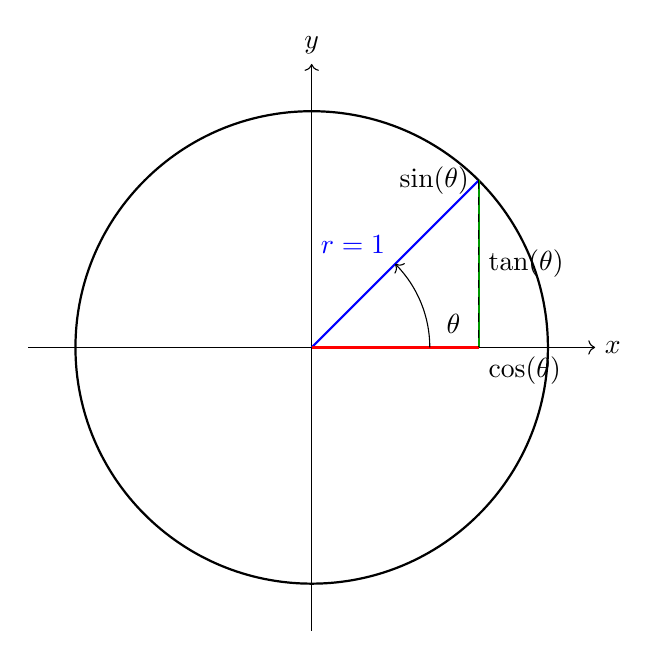
\begin{tikzpicture}[scale=3]
    % Draw unit circle
    \draw[thick] (0,0) circle (1);
    
    % Axes
    \draw[->] (-1.2,0) -- (1.2,0) node[right] {\(x\)};
    \draw[->] (0,-1.2) -- (0,1.2) node[above] {\(y\)};
    
    % Angle and triangle
    \draw[thick, blue] (0,0) -- ({cos(45)},{sin(45)}) node[pos=0.5, above left] {\(r=1\)};
    \draw[thick, red] (0,0) -- ({cos(45)},0);
    \draw[thick, green!60!black] ({cos(45)},0) -- ({cos(45)},{sin(45)});
    
    % Dotted lines
    \draw[dashed] ({cos(45)},{sin(45)}) -- ({cos(45)},0);
    
    % Angle arc
    \draw[->] (0.5,0) arc[start angle=0,end angle=45,radius=0.5];
    \node at (0.6,0.1) {\(\theta\)};
    
    % Labels
    \node[below right] at ({cos(45)},0) {\(\cos(\theta)\)};
    \node[left] at ({cos(45)},{sin(45)}) {\(\sin(\theta)\)};
    \node[right] at ({cos(45)}, {sin(45)/2}) {\(\tan(\theta)\)};
\end{tikzpicture}
\end{center}

\subsection{Definitions on the Unit Circle:}

\begin{itemize}

    \item \(\cos(\theta)\) is the \emph{x-coordinate} of the point on the circle.

    \item \(\sin(\theta)\) is the \emph{y-coordinate}.

    \item \(\tan(\theta) = \dfrac{\sin(\theta)}{\cos(\theta)}\) is the ratio of the opposite side to 
          the adjacent side in the triangle.

\end{itemize}

\subsection{Trigonometric Rules}

\begin{itemize}

    \item \(\frac{\sin \alpha}{a} = \frac{\sin \beta}{b} = \frac{\sin \gamma}{c}\)

    \item \(c^2 = a^2 + b^2 - 2ab \cos \gamma\)

    \item \(\frac{a - b}{a + b} = \frac{\tan \frac{1}{2}(\alpha - \beta)}{\tan \frac{1}{2} (\alpha + \beta)}\)

\end{itemize}

\subsection{Proof of the Cosine Rule}

The \emph{Cosine Rule} relates the lengths of the sides of a triangle to the cosine of one of its angles. 
For any triangle \( ABC \) with sides \( a = BC \), \( b = AC \), and \( c = AB \), and angle 
\( \gamma = \angle ACB \), the cosine rule states:

\[
    c^2 = a^2 + b^2 - 2ab\cos(\gamma)
\]

\textbf{Proof:}

Consider triangle \( ABC \), and place it on the coordinate plane such that point \(c\) is at the origin
\( (0,0) \), point \(B\) is at \( (a,0) \), and point \(A\) lies somewhere in the plane. 
Let angle \( \gamma = \angle ACB \).

Let the coordinates of point \(A\) be \( (b\cos\gamma, b\sin\gamma) \), since \( b = AC \) and we’re 
using polar coordinates to define its location relative to point \(c\).

Using the distance formula to find side \( c = AB \), we get:

\begin{align*}
    c^2 &= {(a - b\cos\gamma)}^2 + {(0 - b\sin\gamma)}^2 \\
    &= a^2 - 2ab\cos\gamma + b^2\cos^2\gamma + b^2\sin^2\gamma \\
    &= a^2 + b^2(\cos^2\gamma + \sin^2\gamma) - 2ab\cos\gamma \\
    &= a^2 + b^2 - 2ab\cos\gamma
\end{align*}

Since \( \cos^2\gamma + \sin^2\gamma = 1 \).

Thus, we have proven that:

\[
    c^2 = a^2 + b^2 - 2ab\cos\gamma
\]

\QED


\newpage
\section{Linear Systems of Equations}

In this section, we will discuss the solution of linear systems of equations. A linear system of
equations is a set of equations that can be expressed in the form:

\begin{align*}
    a_{11}x_1 + a_{12}x_2 + \cdots + a_{1n}x_n & = b_1  \\
    a_{21}x_1 + a_{22}x_2 + \cdots + a_{2n}x_n & = b_2  \\
                                               & \vdots \\
    a_{m1}x_1 + a_{m2}x_2 + \cdots + a_{mn}x_n & = b_m,
\end{align*}

where \( a_{ij} \) are the coefficients of the variables \( x_j \), and \( b_i \) are the constants
on the right-hand side of the equations. The goal is to find the values of \( x_1, x_2, \ldots, x_n \)
that satisfy all equations simultaneously.

\subsection{Matrix Representation}

A linear system can be represented in matrix form as:

\[
    A x = b
\]

Where \(A\) is the coefficient matrix, \(x\) is the vector of variables, and \(b\) is the vector
of constants. The coefficient matrix \(A\) is an \( m \times n \) matrix, where \( m \) is the number
of equations and \(n\) is the number of variables. The vector \(x\) is an \( n \times 1 \) column
vector, and the vector \(b\) is an \( m \times 1 \) column vector.

\subsection{Solution Set of a Linear System}

In the context of Definition 6.1, the solution set \( L(A, b) \) of the system of equations associated
with \( (A, b) \) is defined as

\[
    L(A, b) := \{ x \in \Field^n \mid Ax = b \}.
\]

\subsection{Equality of the Rank \texorpdfstring{\(\operatorname{rg}(A) = \operatorname{rg}_S(A)\)}{}}

We have \(\operatorname{rg}(A) = \operatorname{rg}_S(A)\).

\textbf{Proof:}

For \(x = {(x_1, \ldots, x_n)}^T \in \Field^n\), it holds that

\[
    Ax = \sum_{i=1}^{n} x_i a_i.
\]

It follows that

\[
    \operatorname{rg}(A) = \operatorname{rg}(L_A) = \dim(\img(L_A))
    = \dim\left(\{L_A(x) \mid x \in \Field^n\}\right)
    = \dim\left(\{Ax \mid x \in \Field^n\}\right)
\]

\[
    = \dim\left\{ \sum_{i=1}^{n} x_i a_i \,\middle|\, x_i \in K \right\}
    = \dim(L(a_1, \ldots, a_n)) = \operatorname{rg}_S(A).
\]

\subsection{Solvability of the Linear System \texorpdfstring{\(Ax = b\)}{}}

The linear system \(Ax = b\) is solvable if and only if

\[
    \operatorname{rg}(a_1, \ldots, a_n) = \operatorname{rg}(a_1, \ldots, a_n, b).
\]

More concisely, we write

\[
    \operatorname{rg}(A) = \operatorname{rg}(A, b).
\]

\textbf{Proof:}

We have

\[
    Ax = (a_1, \ldots, a_n)x = x_1 a_1 + \cdots + x_n a_n = b.
\]

Therefore, a solution vector \(x\) exists if and only if

\[
    b \in L(a_1, \ldots, a_n) \quad \Leftrightarrow \quad \operatorname{rg}(A) = \operatorname{rg}(A, b),
\]

where \(L(a_1, \ldots, a_n)\) denotes the linear span of \(a_1, \ldots, a_n\).

\subsection{Solution Set of the Linear System \texorpdfstring{\(Ax = b\)}{}}

Let \(x_s \in \Field^n\) be a solution of \(Ax = b\). Then the solution set is given by

\[
    L(A, b) = x_s + \ker(A) = \{x_s + x \mid x \in \ker(A)\}.
\]

\textbf{Proof:}

\[
    x \in \ker(A) \;\Leftrightarrow\; Ax = 0 \;\Leftrightarrow\; A(x_s + x) = Ax_s + Ax = Ax_s = b.
\]

\subsection{Free Variables}

In a system of linear equations, a \emph{free variable} is a variable whose column in the coefficient
matrix does not correspond to a pivot column after row reduction. Free variables are not directly solved by
any equation in the system; instead, they can take any real value, and the values of the leading
(or dependent) variables are expressed in terms of them.

Free variables arise naturally in systems with infinitely many solutions and play a key role in
describing the solution set. Given a system of with \(p\) equations and \(q\) unknowns then if
\(q > p\) then there are \(q - p\) free variables.

\textbf{Example:}

Consider the system

\[
    \begin{cases}
        x_1 + 2x_2 - x_3 = 4 \\
        3x_1 + 6x_2 - 3x_3 = 12
    \end{cases}
\]

which row reduces to

\[
    \begin{bmatrix}
        1 & 2 & -1 \\
        0 & 0 & 0
    \end{bmatrix}.
\]

Here, the pivot is in the first column corresponding to \( x_1 \), while \( x_2 \) and \( x_3 \) are free
variables. Assigning parameters to \( x_2 \) and \( x_3 \), the general solution can be expressed in terms
of these free variables.

\subsection{Gaussian Elimination}

Gaussian elimination is a method for solving linear systems by transforming the system into an upper
triangular form. The steps involved in Gaussian elimination are:

\begin{enumerate}

    \item Forward elimination: Transform the system into an upper triangular form by eliminating the
          variables from the equations.

    \item Back substitution: Solve for the variables starting from the last equation and substituting
          back into the previous equations.

\end{enumerate}

The forward elimination process involves performing row operations on the augmented matrix
\([A | \mathbf{b}]\) to create zeros below the diagonal. The row operations include:

\begin{itemize}

    \item Swapping two rows

    \item Multiplying a row by a non-zero scalar

    \item Adding or subtracting a multiple of one row from another row

\end{itemize}

Once the matrix is in upper triangular form, back substitution is used to find the values of the
variables. The last equation gives the value of the last variable, which can then be substituted into
the previous equations to find the other variables.

\subsection{Gauss-Jordan Elimination}

Gauss-Jordan elimination is an extension of Gaussian elimination that transforms the matrix into
reduced row echelon form (RREF). In RREF, each leading entry in a row is 1, and all entries above and
below the leading entry are zeros. The steps involved in Gauss-Jordan elimination are:

\begin{enumerate}

    \item Forward elimination: Transform the system into an upper triangular form.

    \item Back substitution: Transform the upper triangular matrix into RREF by eliminating the entries
          above the leading 1s.

    \item Solve for the variables directly from the RREF matrix.

\end{enumerate}

The Gauss-Jordan elimination method is particularly useful for finding the inverse of a matrix, as it 7
can be applied to the augmented matrix \([A | I]\), where \(I\) is the identity matrix. If the left side
of the augmented matrix becomes \(I\), then the right side will be the inverse of \(A\).

\textbf{Example:}

Solve the following system of equations using Gaussian elimination:

\begin{align*}
    2x + 3y + z  & = 1 \\
    4x + y - z   & = 2 \\
    -2x + y + 3z & = 3
\end{align*}

\textbf{Solution:} The augmented matrix for the system is:

\[
    \begin{bmatrix}
        2  & 3 & 1  & | & 1 \\
        4  & 1 & -1 & | & 2 \\
        -2 & 1 & 3  & | & 3
    \end{bmatrix}
\]

Performing row operations to eliminate the variables, we can transform the matrix into upper triangular form:

\[
    \begin{bmatrix}
        1 & \frac{3}{2} & \frac{1}{2} & | & \frac{1}{2} \\
        0 & -5          & -3          & | & 0           \\
        0 & 0           & 1           & | & 1
    \end{bmatrix}
\]

Now, we can perform back substitution to find the values of \(x\), \(y\), and \(z\):

\begin{align*}
    z           & = 1                           \\
    -5y - 3z    & = 0 \implies y = -\frac{3}{5} \\
    2x + 3y + z & = 1 \implies x = \frac{1}{5}
\end{align*}

Thus, the solution to the system is:

\begin{align*}
    x & = \frac{1}{5}  \\
    y & = -\frac{3}{5} \\
    z & = 1
\end{align*}

\subsection{Homogeneous Linear Equations}

A linear equation is said to be \emph{homogeneous} if its constant term is zero. That is, it
can be written in the form:

\[
    a_1 x_1 + a_2 x_2 + \cdots + a_n x_n = 0
\]

Such equations always have at least the trivial solution \(x_1 = x_2 = \cdots = x_n = 0\).

\subsection{Particular Solution}

A particular solution to a linear system of equations is a specific solution that satisfies the system.
It can be found using various methods, including substitution, elimination, or matrix methods. A
particular solution is not unique; there may be multiple particular solutions depending on the system.
A particular solution can be found by substituting specific values for the variables and solving for the
remaining variables. For example, in the system

\begin{align*}
    2x + 3y & = 5 \\
    4x - y  & = 1
\end{align*}

we can substitute \(x = 1\) into the first equation to find \(y\):

\begin{align*}
    2(1) + 3y & = 5 \\
    3y        & = 3 \\
    y         & = 1
\end{align*}

Thus, \((x, y) = (1, 1)\) is a particular solution to the system. However, this is not the only solution;
other values of \(x\) may yield different values of \(y\).

\subsection{General = Particular + Homogeneous}

The general solution of a linear system of equations is the complete set of solutions that satisfy the
system. It can be expressed as the sum of a particular solution and the general solution of the associated
homogeneous system.

The general solution can be written as:

\[
    x = x_p + x_h
\]

Where \( x_p \) is a particular solution to the non-homogeneous system, and \( x_h \) is the general
solution to the homogeneous system. The homogeneous system is obtained by setting the right-hand side
of the equations to zero:

\[
    A x = 0
\]

The theorem says:

Any linear system's solution set has the form:

\[
    \left\{ \vec{p} + c_1\vec{\beta}_1 + \cdots + c_k\vec{\beta}_k \;\middle|\; c_1, \ldots, c_k \in
    \Reals \right\},
\]

where \(\vec{p}\) is a particular solution to the system, and the vectors \(\vec{\beta}_1,
\ldots, \vec{\beta}_k\) form a basis of the solution space to the corresponding homogeneous system.
The number \(k\) equals the number of \textbf{free variables} the system has after applying Gaussian
elimination.

\subsection{Linear Combination Lemma}

Any linear combination of linear combinations is a linear combination.

\subsection{Example: Gaussian Elimination with 3 Equations and 4 Unknowns}

Consider the following system of linear equations:

\begin{align*}
    x_1 + 2x_2 + x_3 + x_4   & = 4  \\
    2x_1 + 5x_2 + x_3 + 3x_4 & = 10 \\
    x_1 + 3x_2 + 2x_3 + 2x_4 & = 7
\end{align*}

\textbf{Step 1: Augmented Matrix}

\[
    \begin{bmatrix}
        1 & 2 & 1 & 1 & 4  \\
        2 & 5 & 1 & 3 & 10 \\
        1 & 3 & 2 & 2 & 7  \\
    \end{bmatrix}
\]

\textbf{Step 2: Eliminate below pivot in column 1}

\begin{itemize}
    \item Row 2 \(=\) Row 2 \(-\) 2 \(\times\) Row 1
    \item Row 3 \(=\) Row 3 \(-\) Row 1
\end{itemize}

\[
    \begin{bmatrix}
        1 & 2 & 1  & 1 & 4 \\
        0 & 1 & -1 & 1 & 2 \\
        0 & 1 & 1  & 1 & 3 \\
    \end{bmatrix}
\]

\textbf{Step 3: Eliminate below pivot in column 2}

\begin{itemize}
    \item Row 3 \(=\) Row 3 \(-\) Row 2
\end{itemize}

\[
    \begin{bmatrix}
        1 & 2 & 1  & 1 & 4 \\
        0 & 1 & -1 & 1 & 2 \\
        0 & 0 & 2  & 0 & 1 \\
    \end{bmatrix}
\]

\textbf{Step 4: Back Substitution}

From Row 3:
\[
    2x_3 = 1 \Rightarrow x_3 = \frac{1}{2}
\]

From Row 2:
\[
    x_2 - x_3 + x_4 = 2 \Rightarrow x_2 = 2 + x_3 - x_4 = 2 + \frac{1}{2} - x_4 = \frac{5}{2} - x_4
\]

From Row 1:
\[
    x_1 + 2x_2 + x_3 + x_4 = 4
    \Rightarrow x_1 = 4 - 2x_2 - x_3 - x_4
\]
Substitute:
\[
    x_1 = 4 - 2\left( \frac{5}{2} - x_4 \right) - \frac{1}{2} - x_4
    = 4 - 5 + 2x_4 - \frac{1}{2} - x_4
    = -1 - \frac{1}{2} + x_4 = -\frac{3}{2} + x_4
\]

\textbf{General Solution}

Let \(x_4 = t\) (free variable), then:

\[
    \begin{aligned}
        x_1 & = -\frac{3}{2} + t \\
        x_2 & = \frac{5}{2} - t  \\
        x_3 & = \frac{1}{2}      \\
        x_4 & = t
    \end{aligned}
    \quad \text{with } t \in \Reals
\]

\textbf{Solution Set:}

\[
    \left\{
    \begin{bmatrix}
        -\frac{3}{2} \\ \frac{5}{2} \\ \frac{1}{2} \\ 0
    \end{bmatrix}
    + t \cdot
    \begin{bmatrix}
        1 \\ -1 \\ 0 \\ 1
    \end{bmatrix}
    \;\middle|\; t \in \Reals
    \right\}
\]

\subsection{The Determinant, the cross product and the solutions of linear Systems of Equations}
A linear system of three equation has the following properties:

\begin{itemize}

    \item There is a unique solution if the determinant of the coefficient matrix is non-zero.

          \[
              \langle (a \times b), c\rangle = \det(a,b,c) \ne 0
          \]

    \item There are infinitely many solutions if the determinant of the coefficient matrix is zero.

          \[
              \langle (a \times b), c\rangle = \det(a,b,c) = 0
          \]

    \item There is no solution if the determinant of the coefficient matrix is zero and the system is inconsistent.

          \[
              \langle (a \times b), c\rangle = 0
          \]

\end{itemize}

\subsection{Chart for the number of solutions}

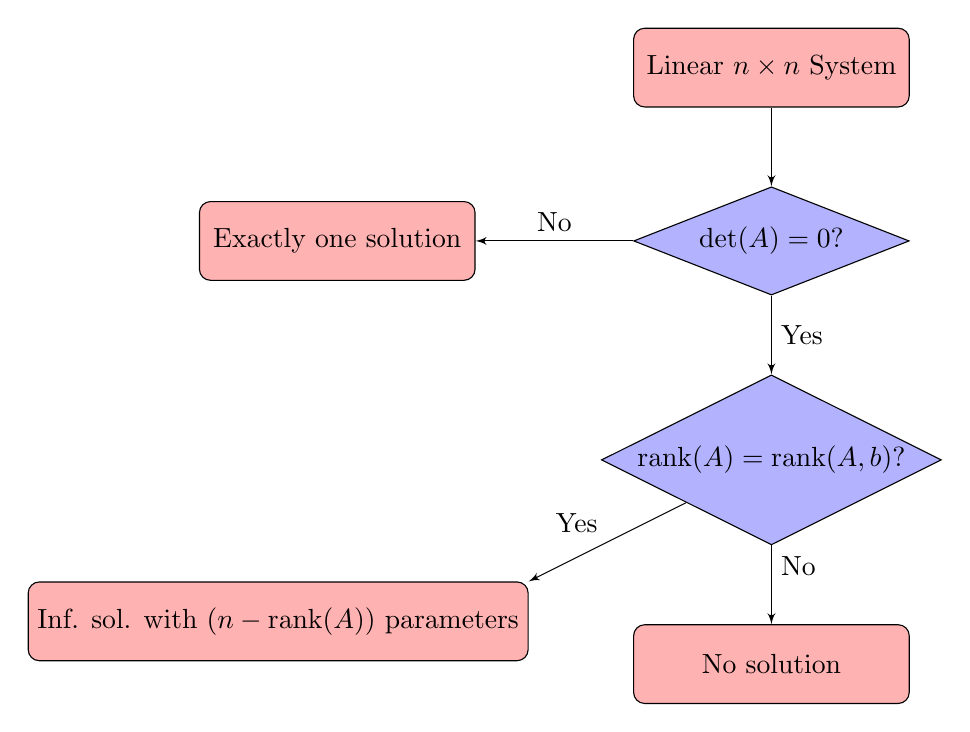
\begin{tikzpicture}[node distance=1cm and 2cm]
    % Nodes
    \node [terminator] (start) {Linear \(n \times n\) System};
    \node [decision, below=of start] (decision1) {\(\det(A) = 0?\)};
    \node [decision, below=of decision1] (decision2) {\(\rank(A) = \rank(A,b)?\)};
    \node [terminator, left=of decision1] (oneS) {Exactly one solution};
    \node [terminator, below left=of decision2] (inS) {Inf. sol. with \((n - \rank(A))\) parameters};
    \node [terminator, below=of decision2] (noS) {No solution};

    % Arrows
    \path [connector] (start) -- (decision1);
    \path [connector] (decision1.west) -- node[above] {No} (oneS.east);
    \path [connector] (decision1) -- node[right] {Yes} (decision2);
    \path [connector] (decision2.south west) -- node[above left] {Yes} (inS.north east);
    \path [connector] (decision2.south) -- node[above right] {No} (noS.north);
\end{tikzpicture}

\bigskip

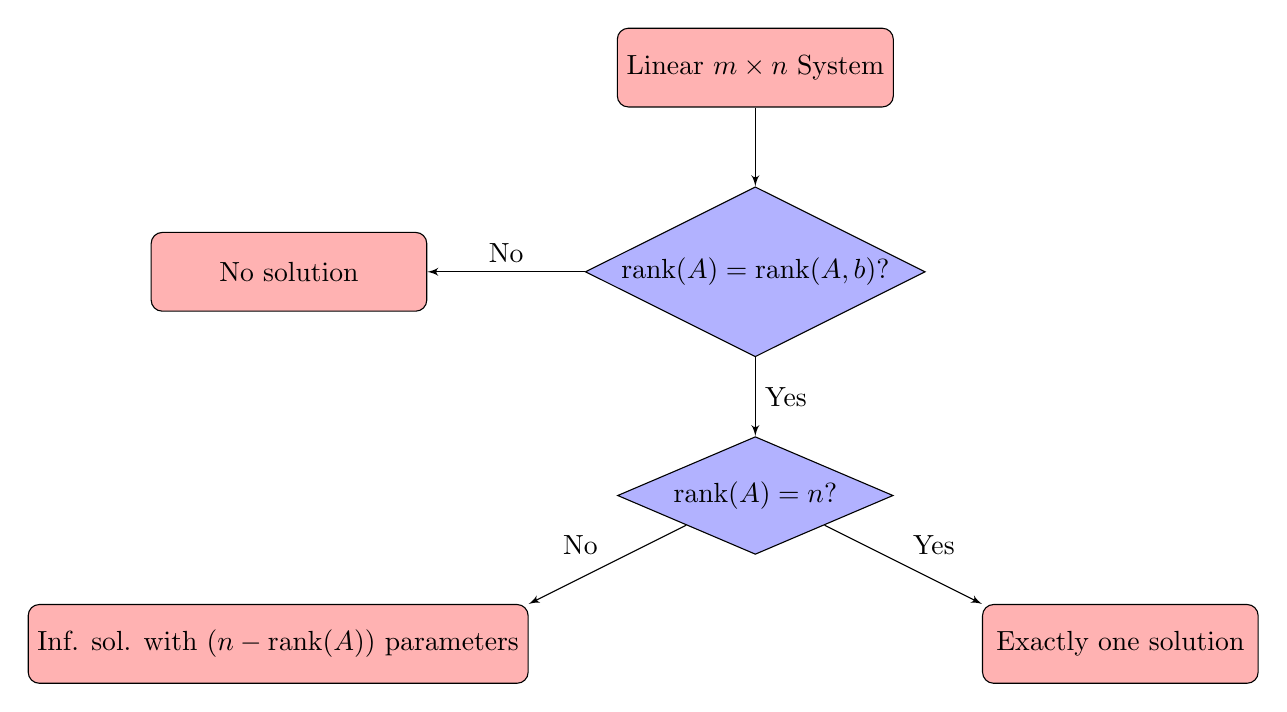
\begin{tikzpicture}[node distance=1cm and 2cm]
    % Nodes
    \node [terminator] (start) {Linear \(m \times n\) System};
    \node [decision, below=of start] (decision1) {\(\rank(A) = \rank(A,b)?\)};
    \node [terminator, left=of decision1] (noS) {No solution};
    \node [decision, below=of decision1] (decision2) {\(\rank(A) = n?\)};
    \node [terminator, below left=of decision2] (inS) {Inf. sol. with \((n - \rank(A))\) parameters};
    \node [terminator, below right=of decision2] (oneS) {Exactly one solution};

    % Arrows
    \path [connector] (start) -- (decision1);
    \path [connector] (decision1.west) -- node[above] {No} (noS.east);
    \path [connector] (decision1) -- node[right] {Yes} (decision2);
    \path [connector] (decision2.south west) -- node[above left] {No} (inS.north east);
    \path [connector] (decision2.south east) -- node[above right] {Yes} (oneS.north west);
\end{tikzpicture}

\subsection{Proof of the Gaussian Elimination}

The row operations do not change the solution set.

\textbf{Proof:}

A linear system of equations of the form \(Ax = b\), \(A \in \Field^{m \times n}\) with some solution
\(x\) can be multiplied by some elementary matrix \(C_1, C_2, C_3\) which correspond to a row
operation \(CAx = Cb\).

The Equality is kept and therefore, \(L(A,b) \subset L(CA, Cb)\). If \(x \in L(CA, Cb)\) then

\[
    CAx = Cb \implies C^{-1}CAx = C^{-1}Cb \implies Ax = b
\]

Because of the invertibility of elementary matrices we can be sure that  \(L(CA, Cb) \subset L(A,b) \).

Now for the case that \(L(A,b) = \emptyset\). If we assume that \(L(CA,CB) \ne \emptyset \), then
there would be some \(x \in L(CA,CB)\) with \(CAx = Cb\). By multiplying both side by \(C^{-1}\) we
get \(Ax = b\) and therefore, \(L(A, b) \ne \emptyset \),  which is a contradiction to our original
assumption  \(L(A,b) = \emptyset\).

\QED

Now we only have to prove that each regular matrix can be transformed in the reduced echelon form or
even row reduced echelon form. This is the equivalent of saying that the row operations do not change
the rank of the matrix.

\textbf{Proof:}

If \(C\) is an elementary matrix and \(A \in \Field^{m \times n}\) some matrix. The statement \(rg(CA) = rg(A)\)
is true because of the invertibility of the elementary matrices and the isomorphism in vector spaces.

Given \(A = (a_1, a_2, \dots, a_n)\). The exchange of two columns preserves \(L := L(a_1, \dots, a_n)\),
and also the \(rg_s (A)\). Concerning the scaling of a column by some \(\lambda \) \(L := L(a_1, \dots, \lambda a_k, \dots, a_n)\)
also preserves \(dim(L) = rg_s(A)\). And finally, the addition \(L = L(a_1, \dots, a_i + \lambda a_k, \dots, a_n)\) also preserves
\(rg_s (A) = rg(A)\). Thus, \(rg(CA) = rg(A)\).

\QED

The only part left is to prove that if \(A\) has an inverse, then with use of the row operations we can
transform it in to a matrix with an upper triangular with also no zero element on the main diagonal.

\textbf{Proof:}

First we eliminate all the elements under the main diagonal for all columns until the column \(k - 1\).
With this, we have created a new matrix \(A^(\ell) = C_{\ell} \dot \cdots \dot C_1 A \) which looks
like:

\[
    A^{(\ell)} =
    \begin{bmatrix}
        a^{(\ell)}_{11} & \cdots & a^{(\ell)}_{1,k-1}   & a^{(\ell)}_{1k}    & a^{(\ell)}_{1,k+1}   & \cdots & a^{(\ell)}_{1n}    \\
        \vdots          & \ddots & \vdots               & \vdots             & \vdots               & \ddots & \vdots             \\
        0               & \cdots & a^{(\ell)}_{k-1,k-1} & a^{(\ell)}_{k-1,k} & a^{(\ell)}_{k-1,k+1} & \cdots & a^{(\ell)}_{k-1,n} \\
        0               & \cdots & 0                    & a^{(\ell)}_{kk}    & a^{(\ell)}_{k,k+1}   & \cdots & a^{(\ell)}_{kn}    \\
        0               & \cdots & 0                    & \vdots             & a^{(\ell)}_{k+1,k+1} & \cdots & a^{(\ell)}_{k+1,n} \\
        \vdots          & \ddots & \vdots               & \vdots             & \vdots               & \ddots & \vdots             \\
        0               & \cdots & 0                    & a^{(\ell)}_{nk}    & \cdots               & \cdots & a^{(\ell)}_{nn}
    \end{bmatrix}
\]

Because of \(rg(A) = rg(A^{(\ell)})\), \(a^{(\ell)}_{ii} \ne 0\) for \(1 \le i < k\). All of these
elements will not change for the rest of the Gaussian Elimination. Now we want to build another matrix
with row operations \(A^{(\mu)}\) where \(a^{(\mu)}_{kk} \ne 0\) and \(a^{(\mu)}_{ik} = 0\) for
\(i > k\). If \(a^{(\ell)}_{kk} \ne 0\) then \((i,k)\)-th element will become 0 by subtracting
\(\frac{a^{(\ell)}_{ik}}{a^{(\ell)}_{kk}}\) time the \(k\)-th row of the \(i\)-th row. So can the \(k\)-th
column be transformed with a series of row operations to the desired form. But if \(a^{(\ell)}_{kk} = 0\),
then you have to swap it with another row under it. This is the critical point of the algorithm: What
if there is no row, also \(a^{(\ell)}_{ik} = 0\) for \(i \ge k\)? Then \(A^{(\ell)}\) would be:

\[
    A^{(\ell)} =
    \begin{bmatrix}
        a^{(\ell)}_{11} & \cdots & a^{(\ell)}_{1,k-1}   & a^{(\ell)}_{1k}    & a^{(\ell)}_{1,k+1}   & \cdots & a^{(\ell)}_{1n}    \\
        \vdots          & \ddots & \vdots               & \vdots             & \vdots               & \ddots & \vdots             \\
        0               & \cdots & a^{(\ell)}_{k-1,k-1} & a^{(\ell)}_{k-1,k} & a^{(\ell)}_{k-1,k+1} & \cdots & a^{(\ell)}_{k-1,n} \\
        0               & \cdots & 0                    & 0                  & a^{(\ell)}_{k,k+1}   & \cdots & a^{(\ell)}_{kn}    \\
        0               & \cdots & 0                    & \vdots             & a^{(\ell)}_{k+1,k+1} & \cdots & a^{(\ell)}_{k+1,n} \\
        \vdots          & \ddots & \vdots               & \vdots             & \vdots               & \ddots & \vdots             \\
        0               & \cdots & 0                    & 0                  & \cdots               & \cdots & a^{(\ell)}_{nn}
    \end{bmatrix}
\]

But, that would imply that the \(k\)-th column is a linear combination of the other \(k - 1\) columns,
and then \(rg(A^{(\ell)}) \le n - 1\) which is a contradiction to the assumption  \(rg(A^{(\ell)}) = n\)

\QED

\subsection{Alternative Method for finding the Rank of a matrix}

For a matrix \(A \in \Field^{(m \times n)}\). The biggest submatrix of the size \(r \times r\) with a
non-zero determinant gives us the \emph{rank} of the matrix. \(rg(A) = r\).

\subsection{Cramer's Rule}

For a square matrix \(A = (a_1, \dots, a_n)\) and \(x,b \in \Field^{n}\) with \(Ax = b\) with \(\det A \ne 0\)
then

\[
    A_i = (a_1, \dots, a_{i - 1}, b, a_{i + 1}, \dots, a_n), i = 1,\dots,n.
\]

The solution \(i\) is then

\[
    x_i = \frac{\det(A_i)}{\det(A)}
\]

\textbf{Proof:}

Given a matrix \(X_i \in \Field^{n \times n}\) by

\[
    \begin{bmatrix}
        1      &   & \cdots    & x_1    &  & \cdots \\
        \vdots &   & \ddots    & \vdots &  & 0      \\
               &   & x_{i - 1} &        &  &        \\
               & 0 & x_i       &        &  &        \\
               &   & x_{i + 1} &        &  &        \\
               &   & \vdots    & \ddots &  &        \\
               &   & x_n       &        &  & 1
    \end{bmatrix}
\]

\(X_i = (e_1, \dots, e_{i - 1}, e_i, e_{i + 1}, \dots, e_n)\). By using an \(n\)-times the
Laplace formula in the first row shows \(|X_i| = x_i\).

\begin{align*}
    A X_i & = A (e_1, \dots, e_{i - 1}, e_i, e_{i + 1}, \dots, e_n)     \\
    A X_i & = A (a_1, \dots, a_{i - 1}, Ax, a_{i + 1}, \dots, a_n)      \\
    A X_i & = A (a_1, \dots, a_{i - 1}, b, a_{i + 1}, \dots, a_n) = A_i
\end{align*}

This implies \(|A_i| = |AX_i| = |A||X_i|\) therefore, \(x_i = \frac{|A_i|}{A}\).

\QED

Another way of thinking about this in a more geometric way is to first think at the determinant as
the area/volume/etc. that is spanned by the basis vector and the stretching factor of the transformation
\(\det(A)\). Now visualize your matrix \(A\) as a linear transformation with
a non-zero determinant and think about \(\det(A_i)\) as the area/volume/etc. which is spanned by the
basis vector but with one of the vector substituted by \(b\).

Now in two dimensions, think of the area spanned by the basis vectors \(A = xy\).
The signed area of the original parallelogram gets
stretched by \(\det(A)\) this gives us \(Area = \det(A)y \Rightarrow y = \frac{Area}{\det(A)}\). This
also works for \(x\).

\input{src/Linear_Algebra/Over_Under_lse.tex}
\newpage
\section{Analytical Geometry}

In this section, we will cover the topics for the geometry of \(\Reals^2\) and \(\Reals^3\).
And maybe also in higher dimensions.

\subsection{Vectors and Points}

In analytical geometry, points and vectors are the basic elements.

A point in \(\Reals^3\) is represented as \(\vec{P} = \begin{bmatrix} x \\ y \\ z \end{bmatrix}\).
Or as \((x_1, x_2, \dots , x_n)\).

A vector is an object with direction and magnitude (in this case), also represented as \(\vec{v} = \begin{bmatrix} v_x \\ v_y \\ v_z \end{bmatrix}\).

Or as \({(x_1, x_2, \dots , x_n)}^{T}\).

\subsection{Vector Addition and Scalar Multiplication}

Given two vectors \(\vec{a}\) and \(\vec{b}\):

\[
	\vec{a} \pm  \vec{b} = \begin{bmatrix} a_x \\ a_y \end{bmatrix} \pm \begin{bmatrix} b_x \\ b_y \end{bmatrix} = \begin{bmatrix} a_x \pm b_x \\ a_y \pm b_y \end{bmatrix}
\]

For a scalar \(\lambda\) and vector \(\vec{a}\):

\[
	\lambda \vec{a} = \lambda \begin{bmatrix} a_x \\ a_y \end{bmatrix} = \begin{bmatrix} \lambda a_x \\ \lambda a_y \end{bmatrix}
\]

\begin{figure}[h!]
	\centering
	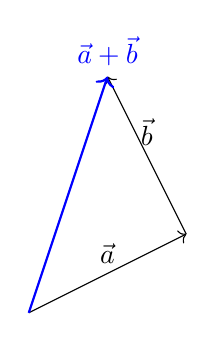
\begin{tikzpicture}
		\draw[->] (0,0) -- (2,1) node[midway, above] {\(\vec{a}\)};
		\draw[->] (2,1) -- (1,3) node[midway, above] {\(\vec{b}\)};
		\draw[->, thick, blue] (0,0) -- (1,3) node[above, above] {\(\vec{a} + \vec{b}\)};
	\end{tikzpicture}
	\caption{Vector addition: \(\vec{a} + \vec{b}\)}
\end{figure}

\subsection{Equation of a Line}

A line is defined by a point \(\vec{P}\) and a direction vector \(\vec{v}\):

\[
	\vec{r}(t) = \vec{P} + t\vec{v}, \quad t \in \Reals
\]

\subsection{Equation of a Plane}

A plane is defined by a point \(\vec{P}\) and a normal vector \(\vec{n}\):

\[
	P: \vec{x} = \vec{s} + \lambda_1 \vec{v_1} + \lambda_2 \vec{v_2}
\]

\subsection{Dot Product}

The inner product of vectors \(\vec{a}\) and \(\vec{b}\) is a function \(\langle x, y\rangle :=V \times V \rightarrow \mathbb{K}\)
with the following properties:

\(\forall \vec{a}, \vec{b} \in V\):

\begin{itemize}

    \item \(\langle\vec{a}, \vec{b}\rangle = \langle\vec{b}, \vec{a}\rangle \)
	
    \item \(\langle\vec{a}, \vec{b} + \vec{c}\rangle = \langle\vec{a}, \vec{b}\rangle + \langle\vec{a}, \vec{c}\rangle\)
	
    \item \(\langle\vec{a}, \lambda \vec{b}\rangle = \lambda \langle\vec{a}, \vec{b}\rangle\)
	
    \item \(\langle\vec{a}, \vec{b}\rangle = 0 \Leftrightarrow \vec{a} = \vec{0} \vee \vec{b} = \vec{0}\)

\end{itemize}

Formula:

\[
	\langle\vec{a}, \vec{b}\rangle = a_1 b_1 + a_2 b_2 + \cdots + a_n b_n = \sum_{i = 1}^{n} a_i b_i
\]

\textbf{Proof:}

Let us look at the following Triangle:

\begin{center}
	\begin{tikzpicture}
		\draw [<->](0, 3) -- (0, -3);
		\draw [<->](3, 0) -- (-3, 0);
		\draw [->, red] (0, 0) -- (2, 2) node[above]{\(\vec{v}\)};
		\draw [->, blue] (0, 0) -- (2, 0) node[above right]{\(\vec{u}\)};
		\draw [->] (2,0) -- (2,2) node[midway, right]{\(\vec{v} - \vec{u}\)};
	    \draw [green, thick] (0.5,0) arc (0:45:0.5) node[midway, right] {\(\theta = 45\)};
	\end{tikzpicture}
\end{center}

We can use the Cosine law: \(\|v - u\|^{2} = \|v\|^2 + \|u\|^2  - 2 \|u\| \|v\| \cos\theta\).

Now we expand:

\[
	\|u\|^2 = u_{1}^2 + u_{2}^2\ \text{ and } \|v\|^2 = v_{1}^2 + v_{2}^2
\]

Then: \(\|v - u\|^2 = {(v_1 - u_1)}^2 + {(v_2 - u_2)}^2\) and by re-grouping after expansion we get

\[
	\langle v, u\rangle = v_1u_1 + v_2u_2 = \|v\|\|u\|\cos \theta \\ 
\]

\QED

And if we manipulates this expression we can also prove the angle formulas.
And with that information we can prove that

\[
	\cos \frac{\pi}{2}\ = \frac{\langle v, u\rangle}{\|v\|\|u\|} = 0
\]

Only if the Dot Product is equal to zero so, like that we have also proved that
only orthogonal vector have a dot product of zero.

\subsubsection{Dot Product as Projection}

The dot product of two vectors can be interpreted as projecting one onto another and 
then multiplying the length of the projecting to the magnitude of the other. For real vectors.

This comes from the fact that taking a dot product of real vectors is the same as 
multiplying one of them with the linear transformation formed by the transpose version of the other vector. 

The transformation will take a vector from our space and take it to the number line and it is also 
linear. In our case,

\[
    \operatorname{Proj} =
    \begin{bmatrix}
        u_{x_1} & u_{x_2} & \cdots & u_{x_n} 
    \end{bmatrix}
\]

is defined this way because when we project our basis vector \(\vec{b}_i\) onto the line our vector \(\vec{u}\) 
because of the symmetry we will get the same value as if we were projecting \(\vec{u}\) onto 
the line \(\vec{b}_i\) lives in.

\subsection{Norm of a Vector}

The norm of a vector \(\vec{a}\) is described by different norms:

It also has the following properties:

\begin{itemize}

	\item \(\|\vec{a}\| \geq 0\) and \(\|\vec{a}\| = 0 \Leftrightarrow \vec{a} = \vec{0}\)

	\item \(\|\lambda \vec{a}\| = |\lambda| \|\vec{a}\|\)

	\item \(\|\vec{a} + \vec{b}\| \leq \|\vec{a}\| + \|\vec{b}\|\) (Triangle inequality)

	\item \(\|\vec{a} + \vec{b}\|^2 = \|\vec{a}\|^2 + \|\vec{b}\|^2 + 2\langle\vec{a}, \vec{b}\rangle\) (Pythagorean theorem)

\end{itemize}

These are the most common norms, although we will be using primarily the euclidean norm:

\begin{itemize}

	\item \emph{Euclidean norm}:
	      \[
		      \|\vec{a}\| = \sqrt{\langle\vec{a}, \vec{a}\rangle} = \sqrt{a_1^2 + a_2^2 + \cdots + a_n^2}
	      \]
	\item \emph{Manhattan norm}:
	      \[
		      \|\vec{a}\|_1 = |a_1| + |a_2| + \cdots + |a_n|
	      \]
	\item \emph{Maximum norm}:
	      \[
		      \|\vec{a}\|_\infty = \max(|a_1|, |a_2|, \dots , |a_n|)
	      \]
\end{itemize}

\subsection{Angle Relations}

The angle \(\theta\) between two vectors is:

\[
	\cos\theta = \frac{\langle\vec{a}, \vec{b}\rangle}{\|\vec{a}\|\|\vec{b}\|}, \quad \theta = \arccos\left( \frac{\langle\vec{a}, \vec{b}\rangle}{\|\vec{a}\|\|\vec{b}\|} \right)
\]

\subsubsection{Line-Line Angle}

Use direction vectors \(\vec{v}_1\) and \(\vec{v}_2\):

\[
	\theta = \arccos\left( \frac{\langle\vec{v}_1, \vec{v}_2\rangle}{\|\vec{v}_1\|\|\vec{v}_2\|} \right)
\]

\subsubsection{Line-Plane Angle}

Let \(\vec{v}\) be the line's direction and \(\vec{n}\) the plane's normal:

\[
	\theta = \arcsin\left( \frac{\langle\vec{v}, \vec{n}\rangle}{\|\vec{v}\|\|\vec{n}\|} \right)
\]

\subsubsection{Plane-Plane Angle}

Angle between planes is angle between their normals:

\[
	\theta = \arccos\left( \frac{\langle\vec{n}_1, \vec{n}_2\rangle}{\|\vec{n}_1\|\|\vec{n}_2\|} \right)
\]

\subsection{Line Relations}

Two lines can be:

\begin{itemize}

	\item \emph{Identical}: same direction vector and point

	\item \emph{Parallel}: direction vectors are proportional

	\item \emph{Intersecting}: one solution for \(t_1\), \(t_2\) such that \(\vec{r}_1(t_1) = \vec{r}_2(t_2)\)

	\item \emph{Skew}: not parallel, do not intersect

\end{itemize}

To find the relation:

\begin{enumerate}

	\item Check if direction vectors are scalar multiples \(\Rightarrow\) parallel

	\item Solve \(\vec{P}_1 + t\vec{v}_1 = \vec{P}_2 + s\vec{v}_2\) for \(t\) and \(s\):

	\begin{itemize}

		\item Solution exists \(\Rightarrow\) intersect

		\item No solution \(\Rightarrow\) skew

	\end{itemize}

	\item If same point and direction vector \(\Rightarrow\) identical

\end{enumerate}

\subsection{Normalization of a vector}

To normalize a vector \(\vec{a}\), we divide it by its length:

\[
	\hat{\vec{a}} = \frac{\vec{a}}{\|\vec{a}\|} = \frac{\begin{bmatrix} a_x \\ a_y \\ a_z \end{bmatrix}}{\sqrt{a_x^2 + a_y^2 + a_z^2}} = \begin{bmatrix} \frac{a_x}{\|\vec{a}\|} \\ \frac{a_y}{\|\vec{a}\|} \\ \frac{a_z}{\|\vec{a}\|} \end{bmatrix}
\]

\subsection{Orthogonal Vectors and the Orthogonal Projection}

Two vectors \(\vec{a}\) and \(\vec{b}\) are orthogonal if:

\[
	\langle\vec{a}, \vec{b}\rangle = 0
\]

The orthogonal projection of vector \(\vec{a}\) onto vector \(\vec{b}\) is given by:

\[
	\text{p}_{\vec{b}}(\vec{a}) = \frac{\langle\vec{a}, \vec{b}\rangle}{\|\vec{b}\|^2} \cdot \vec{b}
\]

\textbf{Proof of the projection formula}

\begin{align*}
	p \| q \implies \alpha q &= p\ \forall \alpha \in \mathbb{K}\ \text{and}\ \forall\ p, q \in V\\
	\langle a - p, q\rangle &= 0 \implies \langle a - \alpha q, q\rangle = 0 \implies \langle a, q\rangle - \alpha \langle q, q\rangle = 0\\
	\alpha &= \frac{\langle a, q\rangle}{\langle q, q\rangle}
\end{align*}

Therefore, the orthogonal projection of vector \(\vec{a}\) on \(\vec{b}\) is given by
multiplying \(\vec{b}\) by the scalar \(\alpha\).

\QED

\begin{figure}[H]
	\centering
	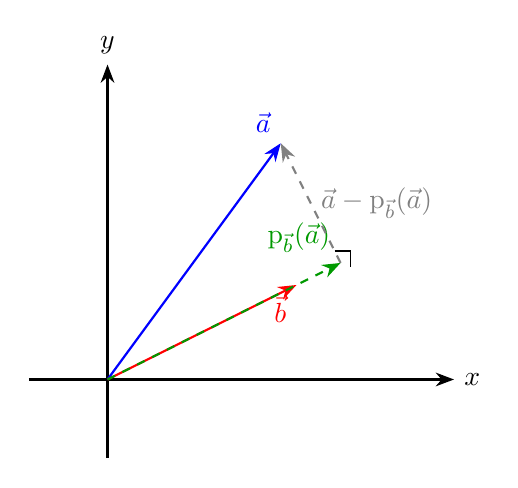
\begin{tikzpicture}[scale=2, >=Stealth]

		% Axes
		\draw[->, thick] (-0.5, 0) -- (2.2, 0) node[right] {\(x\)};
		\draw[->, thick] (0, -0.5) -- (0, 2) node[above] {\(y\)};

		% Coordinates
		\coordinate (O) at (0,0);
		\coordinate (A) at (1.1,1.5);       % vector a
		\coordinate (B) at (1.2,0.6);       % vector b
		\coordinate (P) at (1.48,0.74);     % projection of a onto b

		% Vectors
		\draw[->, thick, blue] (O) -- (A) node[above left] {\(\vec{a}\)};
		\draw[->, thick, red] (O) -- (B) node[below left] {\(\vec{b}\)};
		\draw[->, thick, green!60!black, dashed] (O) -- (P) node[above left] {\(\text{p}_{\vec{b}}(\vec{a})\)};

		% Orthogonal component
		\draw[->, thick, gray, dashed] (P) -- (A) node[midway, right] {\(\vec{a} - \text{p}_{\vec{b}}(\vec{a})\)};

		% Right angle marker
		\draw ($(P)!0.1!(A)$) -- ++(0.1,0) -- ++(0,-0.1);

	\end{tikzpicture}
	\caption{Orthogonal projection of \(\vec{a}\) onto \(\vec{b}\)}
\end{figure}

\subsection{The Cross Product}

The cross product of two vectors \(\vec{a}\) and \(\vec{b}\) in \(\Reals^3\) is defined as:

\[
	\vec{a} \times \vec{b} = \begin{bmatrix} a_1 \\ a_2 \\ a_3 \end{bmatrix} \times \begin{bmatrix} b_1 \\ b_2 \\ b_3 \end{bmatrix} = \begin{bmatrix} a_2 b_3 - a_3 b_2 \\ a_3 b_1 - a_1 b_3 \\ a_1 b_2 - a_2 b_1 \end{bmatrix}
\]

or 

\[
	\det\left( \begin{bmatrix}
		\imath & v_1 & w_1 \\
		\jmath & v_2 & w_2 \\
		\hat{k} & v_3 & w_3
	\end{bmatrix} \right)
	= \imath (v_2 w_3 - v_3 w_2) - \jmath (v_1 w_3 - v_3 w_1) + \hat{k}(v_1 w_2 - v_2 w_1)
\]

The cross product has the following properties:

\begin{itemize}

	\item \(\vec{a} \times \vec{b} = -(\vec{b} \times \vec{a})\)

	\item \(\vec{a} \times (\vec{b} + \vec{c}) = \vec{a} \times \vec{b} + \vec{a} \times \vec{c}\)

	\item \((\lambda_1\vec{a}) \times (\lambda_2\vec{b}) = \lambda_1\lambda_2(\vec{a} \times \vec{b})\)

	\item \(\|\vec{a} \times \vec{b}\| = \|\vec{a}\|\|\vec{b}\| \sin(\theta)\)

	\item \(\langle\vec{a}, (\vec{b} \times \vec{c})\rangle = 0\) (scalar triple product)

	\item \(\vec{a} \times \vec{b} = \vec{0} \Leftrightarrow \vec{a} = \lambda\vec{b}\) for some \(\lambda \in \Reals\) (parallel vectors)

	\item \(\vec{a} \times \vec{b} = \vec{0} \Leftrightarrow \vec{a} = \vec{0} \vee \vec{b} = \vec{0}\) (zero vector)

\end{itemize}

The cross product is not defined in \(\Reals^2\).
The cross product is not commutative, but it is associative:

\[
	(\vec{a} \times \vec{b}) \times \vec{c} = \vec{a} \times (\vec{b} \times \vec{c})
\]

The cross product is distributive over vector addition:

\[
	\vec{a} \times (\vec{b} + \vec{c}) = \vec{a} \times \vec{b} + \vec{a} \times \vec{c}
\]

The cross product is anti-commutative:

\[
	\vec{a} \times \vec{b} = -(\vec{b} \times \vec{a})
\]

The cross product is not associative:

\[
	(\vec{a} \times \vec{b}) \times \vec{c} \neq \vec{a} \times (\vec{b} \times \vec{c})
\]

The cross product is not distributive over scalar multiplication:

\[
	\lambda(\vec{a} \times \vec{b}) \neq (\lambda\vec{a}) \times \vec{b}
\]

The length of the cross product in \(\Reals^3\) is the area of the parallelogram spanned by the two vectors.

\subsubsection{Determinant Trick}

For two vectors \(\vec{a}\) \(\vec{b}\) in \(\Complex^3\) we can compute the cross product by: 

\[
    \vec{n} = 
    \begin{bmatrix}
        \hat{i} & \hat{j} & \hat{k} \\ 
        a_1 & a_2 & a_3 \\ 
        b_1 & b_2 & b_3 
    \end{bmatrix}
\]

\subsubsection{Connection to the Volume of the Parallelepiped}

We want to define a linear transformation \(f\) which relates the volume of the parallelepiped formed by three vectors, the determinant; and 
the dot product of a input vector of the transformation with some vector \(\vec{p}\).  

\[
    f \left(
    \begin{bmatrix}
       x \\ y \\ z 
    \end{bmatrix}
    \right)
    = \det 
    \left(
        \begin{bmatrix}
            x & v_1 & w_1 \\ 
            y & v_2 & w_2 \\ 
            z & v_3 & w_3 
        \end{bmatrix}
    \right)
    =
    \left\langle
    \begin{bmatrix}
       p_1 \\ p_2 \\ p_3 
    \end{bmatrix}
    ,
    \begin{bmatrix}
       x \\ y \\ z 
    \end{bmatrix}
    \right\rangle
\]

This gives us another version of the determinant trick view previously and we know that this gives us a vector perpendicular to \(\vec{v}\) and 
\(\vec{w}\). The motivation behind this weird formula is that if you compute both sides of the equation you will get the coordinates \(\vec{p}\) 
from the determinant trick. 

This whole equality can be related to the geometric meaning of the cross product. Remember that the dot product of two vectors can be 
interpreted as projecting one onto another and then multiplying the length of the projecting to the magnitude of the other. This is exactly the same 
as projecting our input vector to a line which is perpendicular to the parallelogram and then multiplying it by the area which will gives us the 
volume. 

\subsubsection{Derivation of the formula}

We define \(\vec{n}\) as a vector perpendicular to \(\vec{v}\) and \(\vec{w}\). Therefore, 

\[
    \vec{v} \cdot \vec{n} = 0 \quad \text{and} \quad \vec{w} \cdot \vec{n} = 0
\]

Writing this out in components, let \(\vec{v} = (v_1, v_2, v_3)\), \(\vec{w} = (w_1, w_2, w_3)\), and \(\vec{n} = (n_1, n_2, n_3)\). Then:

\[
    v_1 n_1 + v_2 n_2 + v_3 n_3 = 0
\]
\[
    w_1 n_1 + w_2 n_2 + w_3 n_3 = 0 
\]

Now we multiply the first equation by \(-w_1\), the second by \(v_1\) and add them 

\[
    n_2(w_2 v_1 - v_2 w_1) + n_3(w_3 v_1 - v_3 w_1) = 0  
\]

We know that the equation \(p c_1 + q c_2 = 0\) has the results \(c_1 = -q\) and \(c_2 = p\). Thus, 

\[
    n_2 =  v_3 w_1 + w_3 v_1
\]
\[
    n_3 = v_1 w_2 - w_1 v_2  
\]

Finally, by substituting into the original equation and solving we get 

\[
    n_1 = v_2 w_3 - v_3 w_2 
\]

Thus, we have gotten the formula for the cross product. 

\QED

\subsection{Orthogonal vectors in \texorpdfstring{\(\Reals^2\ \Reals^3\)}{}}

\subsubsection{Orthogonal vectors in \texorpdfstring{\(\Reals^2\)}{}}

\begin{enumerate}
	\item Interchange the components
	\item Change the sign of one component
\end{enumerate}

\subsubsection{Orthogonal vectors in \texorpdfstring{\(\Reals^3\)}{}}
\begin{enumerate}
	\item Interchange two components
	\item the one that was not changed, set to zero
	\item Change the sign of first component
\end{enumerate}

\textbf{Example:}

\[
	\vec{a} = \begin{bmatrix} 1 \\ 2 \\ 3 \end{bmatrix}, \quad \vec{b} = \begin{bmatrix} -2 \\ 1 \\ 0 \end{bmatrix}
\]

\subsection{Hessian Normal Form}

The Hessian normal form is a way of expressing the equation of a plane in three-dimensional space using a normalized normal vector. It is particularly useful in computational geometry and physics, where signed distances from points to planes are important.

\subsubsection{Geometric Interpretation}

The Hessian normal form represents a plane by specifying:

\begin{itemize}
	
	\item A unit normal vector \(\vec{n} = (a, b, c)\) to the plane,

	\item and the shortest distance \(d\) from the origin to the plane.

\end{itemize}

This form is derived by normalizing the general plane equation. A plane in 3D can be written as:

\[
	ax + by + cz + d = 0,
\]

where \((a, b, c)\) is a normal vector to the plane and \(d\) is the dot product of the normal vector with a point \(p\).
If we divide all terms by \(\sqrt{a^2 + b^2 + c^2}\), we normalize the normal vector:

\[
	\frac{a}{\sqrt{a^2 + b^2 + c^2}}x + \frac{b}{\sqrt{a^2 + b^2 + c^2}}y + \frac{c}{\sqrt{a^2 + b^2 + c^2}}z + \frac{d}{\sqrt{a^2 + b^2 + c^2}} = 0.
\]

Let:

\[
	\vec{n} = \left(\frac{a}{\sqrt{a^2 + b^2 + c^2}}, \frac{b}{\sqrt{a^2 + b^2 + c^2}}, \frac{c}{\sqrt{a^2 + b^2 + c^2}}\right), \quad d' = \frac{d}{\sqrt{a^2 + b^2 + c^2}},
\]

then the equation becomes:

\[
	\vec{n} \cdot \vec{r} + d' = 0,
\]

which is the Hessian normal form. Here, \(\vec{r} = (x, y, z)\) is any point on the plane, and \(\vec{n}\) is the unit normal.

\subsubsection{Signed Distance to the Plane}

This form allows easy calculation of the signed distance from any point \(\vec{p}\) to the plane:

\[
	\text{distance} = \vec{n} \cdot \vec{p} + d',
\]

which is positive if \(\vec{p}\) lies on the same side of the plane as the normal vector.

\subsubsection{Derivation Illustration}

To visualize the derivation, imagine a plane with unit normal vector \(\vec{n}\), and a point \(P\) in space. The shortest distance from \(P\) to the plane is the projection of the vector \(\vec{p} - \vec{q}\) onto \(\vec{n}\), where \(\vec{q}\) is any point on the plane. This leads to:

\[
	\text{distance} = (\vec{p} - \vec{q}) \cdot \vec{n}.
\]

This gives the signed distance formula and thus, motivates the Hessian form.

\subsection{Converting from the parametric form to the Hessian normal form}

Steps:

\begin{enumerate}

	\item Find the normal vector \(\vec{n}\) of the plane
	
	\item Normalize the normal vector
	
	\item Find the distance \(d\) from the origin to the plane
	
	\item Write the Hessian normal form

\end{enumerate}

\subsection{Converting from the Hessian normal form to the parametric form}

Steps:

\begin{enumerate}

	\item Find a point on the plane

	\item Find two direction vectors in the plane

	\item Write the parametric form

\end{enumerate}

\subsection{Properties of lines and planes}

\begin{itemize}

	\item Two planes are parallel if their normal vectors are scalar multiples of each other.

	\item A line and a plane are parallel if the direction vector of the line is orthogonal to the normal vector of the plane.

	\item A line intersects a plane if there exists a point on the line that satisfies the equation of the plane.

	\item Two planes intersect in a line if their normal vectors are not parallel.

	\item Three planes can intersect in a point, a line, or not at all.

	\item If we have a line \(G\) and a point on the line, for every vector \(\vec{n}\) that is orthogonal to the
 	      direction vector of the line: \(x \in G \iff \langle x, n \rangle\)

	\item If \(p\) and \(q\) are two points in the line \(G\) with a normal vector then \(\langle p, n\rangle = \langle q, n\rangle\)

	\item Let \(E\) be a plane with the origin \(p\) and the direction vector \(\vec{v}\) and \(\vec{w}\), then there exist a normal vector and
	      \(x \in E \iff \langle x, n\rangle = \langle p, n \rangle\)

\end{itemize}

\subsection{Convert Normal Vector in Two Direction Vectors}

Steps:

\begin{enumerate}
	
	\item Given the normal vector \(\vec{n} = (a, b, c)\), interchange \(a\) and \(b\) and multiply \(b\) by -1
	
	\item Set the other component to 0. This gives you the first direction vector \(\vec{v} = (-b, a, 0)\)
	
	\item Take the original normal vector \(\vec{n}\) and interchange \(a\) and \(c\) and multiply \(c\) by -1
	
	\item Set the other component to 0. This gives you the second direction vector \(\vec{w} = (-c, 0, a)\)

\end{enumerate}

\subsection{Intersection between Line and Plane}

To find the intersection between a line and a plane, we can use the following steps:

\begin{enumerate}

	\item Write the parametric form of the line: \(\vec{r}(t) = \vec{P} + t\vec{v}\), where \(\vec{P}\) is a point on the line and \(\vec{v}\) is the direction vector.

	\item Write the equation of the plane in Hessian normal form: \(\langle \vec{n}, \vec{x} - \vec{P} \rangle = 0\), where \(\vec{n}\) is the normal vector and \(\vec{P}\) is a point on the plane.

	\item Substitute the parametric form of the line into the equation of the plane.

	\item Solve for \(t\) to find the intersection point.

	\item Substitute \(t\) back into the parametric form of the line to find the intersection point.

\end{enumerate}

\textbf{Example:}

Given the line:

\[
	g(t) = \begin{bmatrix} 0 \\ 0 \\ 1 \end{bmatrix} + t \begin{bmatrix} 1 \\ 1 \\ 1 \end{bmatrix}
\]

and the plane:

\[
	E(u, m) = \begin{bmatrix} 0 \\ 1 \\ 2 \end{bmatrix} + u \begin{bmatrix} 1 \\ 0 \\ 1 \end{bmatrix} + m \begin{bmatrix} 1 \\ 1 \\ 0 \end{bmatrix},
\]

we want to find the intersection point.

\textbf{Step 1:} Determine the normal vector of the plane using the cross product of the two direction vectors:

\[
	\vec{v}_1 = \begin{bmatrix} 1 \\ 0 \\ 1 \end{bmatrix}, \quad \vec{v}_2 = \begin{bmatrix} 1 \\ 1 \\ 0 \end{bmatrix}
\]

\[
	\vec{n} = \vec{v}_1 \times \vec{v}_2 =
	\begin{bmatrix} 1 \\ 0 \\ 1 \end{bmatrix} \times \begin{bmatrix} 1 \\ 1 \\ 0 \end{bmatrix} =
	\begin{bmatrix} -1 \\ 1 \\ 1 \end{bmatrix}
\]

\textbf{Step 2:} Use the normal vector and a point on the plane to write the plane equation:

\[
	\langle \vec{n}, \vec{x} - \vec{Q} \rangle = 0, \quad \vec{Q} = \begin{bmatrix} 0 \\ 1 \\ 2 \end{bmatrix}
\]

\textbf{Step 3:} Plug the line into the plane equation:

\[
	\vec{x}(t) = \begin{bmatrix} 0 \\ 0 \\ 1 \end{bmatrix} + t \begin{bmatrix} 1 \\ 1 \\ 1 \end{bmatrix}
	\Rightarrow
	\vec{x}(t) - \vec{Q} =
	\begin{bmatrix} t \\ t - 1 \\ t - 1 \end{bmatrix}
\]

Now compute the dot product:

\[
	\langle \vec{n}, \vec{x}(t) - \vec{Q} \rangle =
	\begin{bmatrix} -1 \\ 1 \\ 1 \end{bmatrix} \cdot \begin{bmatrix} t \\ t - 1 \\ t - 1 \end{bmatrix}
	= -t + (t - 1) + (t - 1) = t - 2
\]

\textbf{Step 4:} Solve for \(t\):

\[
	t - 2 = 0 \Rightarrow t = 2
\]

\textbf{Step 5:} Substitute \( t = 2 \) into the line:

\[
	\vec{x}(2) = \begin{bmatrix} 0 \\ 0 \\ 1 \end{bmatrix} + 2 \begin{bmatrix} 1 \\ 1 \\ 1 \end{bmatrix} =
	\begin{bmatrix} 2 \\ 2 \\ 3 \end{bmatrix}
\]

\textbf{Result:} The line intersects the plane at the point

\[
	\begin{bmatrix} 2 \\ 2 \\ 3 \end{bmatrix}
\]

\textbf{Proof:}

\[
	E: \langle x, n\rangle = \langle p, n \rangle
\]
\[
	G: x = p + t \cdot v
\]
\[
	\langle x, n \rangle = c
\]
\[
	\langle p + t \cdot v, n \rangle = c
\]
\[
	\langle p, n \rangle + t \cdot \langle v, n \rangle = c
\]
\[
	t = \frac{c - \langle p, n \rangle}{\langle v, n \rangle}
\]
\QED

\subsection{Distances between points, lines and planes}

\subsubsection{Distance between two points}

The distance between two points \(\vec{P_1}\) and \(\vec{P_2}\) in \(\Reals^n\) is given by:
\[
	d(\vec{P_1}, \vec{P_2}) = \|\vec{P_1} - \vec{P_2}\| = \sqrt{{(x_1 - x_2)}^2 + {(y_1 - y_2)}^2 + \cdots + {(z_1 - z_2)}^2}
\]
where \(\vec{P_1} = (x_1, y_1, \dots,z_1)\) and \(\vec{P_2} = (x_2, y_2, \dots,z_2)\).

\subsubsection{Distance between a point and a hyperplane}

The distance between a point \(\vec{P}\) and a hyperplane defined by the equation \(\langle \vec{n}, \vec{x} - \vec{P_0} \rangle = 0\) is given by:

\[
	d(\vec{P}, \text{hyperplane}) = \frac{|\langle \vec{n}, \vec{P} - \vec{P_0} \rangle|}{\|\vec{n}\|}
\]

where \(\vec{P_0}\) is a point on the hyperplane and \(\vec{n}\) is the normal vector of the hyperplane.

\subsubsection{Distance between two lines}

The distance between two lines in \(\Reals^3\) can be calculated using the formula:

\[
	d = \frac{|\langle \vec{v_1} \times \vec{v_2}, \vec{P_2} - \vec{P_1} \rangle|}{\|\vec{v_1} \times \vec{v_2}\|}
\]

where \(\vec{P_1}\) and \(\vec{P_2}\) are points on the two lines, and \(\vec{v_1}\) and \(\vec{v_2}\) are the direction vectors of the lines.

\subsubsection{Distance between a point and a line}

The distance between a point \(\vec{P}\) and a line defined by the parametric equation \(\vec{r}(t) = \vec{P_0} + t\vec{v}\) is given by:

\[
	d(\vec{P}, \text{line}) = \frac{\|\vec{v} \times (\vec{P} - \vec{P_0})\|}{\|\vec{v}\|}
\]

where \(\vec{P_0}\) is a point on the line and \(\vec{v}\) is the direction vector of the line.

\subsubsection{Distance between two planes}

The distance between two parallel planes defined by the equations \(\langle \vec{n}, \vec{x} - \vec{P_1} \rangle = 0\) and \(\langle \vec{n}, \vec{x} - \vec{P_2} \rangle = 0\) is given by:

\[
	d = \frac{|\langle \vec{n}, \vec{P_2} - \vec{P_1} \rangle|}{\|\vec{n}\|}
\]

where \(\vec{P_1}\) and \(\vec{P_2}\) are points on the two planes, and \(\vec{n}\) is the normal vector of the planes.

\subsubsection{Distance between a point and a plane}

The distance between a point \(\vec{P}\) and a plane defined by the equation \(\langle \vec{n}, \vec{x} - \vec{P_0} \rangle = 0\) is given by:

\[
	d(\vec{P}, \text{plane}) = \frac{|\langle \vec{n}, \vec{P} - \vec{P_0} \rangle|}{\|\vec{n}\|}
\]

where \(\vec{P_0}\) is a point on the plane and \(\vec{n}\) is the normal vector of the plane.

\textbf{Example:}

Distance Between Two Skew Lines

To find the shortest distance between two skew lines, we use the formula:

\[
	\text{distance} = \frac{|\langle(\vec{P}_2 - \vec{P}_1), (\vec{v}_1 \times \vec{v}_2)\rangle|}{\|\vec{v}_1 \times \vec{v}_2\|}
\]

Where:

\begin{itemize}

	\item \(\vec{P}_1\) and \(\vec{P}_2\) are points on each line,

	\item \(\vec{v}_1\) and \(\vec{v}_2\) are the direction vectors,

	\item \(\vec{v}_1 \times \vec{v}_2\) is the cross product of the direction vectors.

\end{itemize}

\textbf{Given:}

\[
	g_1: \vec{r}_1(a) = \begin{bmatrix} 2 \\ 2 \\ 2 \end{bmatrix} + a \begin{bmatrix} 0 \\ 1 \\ 1 \end{bmatrix}, \quad
	g_2: \vec{r}_2(b) = \begin{bmatrix} 1 \\ 2 \\ 3 \end{bmatrix} + b \begin{bmatrix} 3 \\ 2 \\ 1 \end{bmatrix}
\]

\textbf{Step 1:} Set

\[
	\vec{P}_1 = \begin{bmatrix} 2 \\ 2 \\ 2 \end{bmatrix}, \quad \vec{v}_1 = \begin{bmatrix} 0 \\ 1 \\ 1 \end{bmatrix}
\]
\[
	\vec{P}_2 = \begin{bmatrix} 1 \\ 2 \\ 3 \end{bmatrix}, \quad \vec{v}_2 = \begin{bmatrix} 3 \\ 2 \\ 1 \end{bmatrix}
\]

\textbf{Step 2:} Compute the vector between base points:

\[
	\vec{P}_2 - \vec{P}_1 = \begin{bmatrix} 1 - 2 \\ 2 - 2 \\ 3 - 2 \end{bmatrix} = \begin{bmatrix} -1 \\ 0 \\ 1 \end{bmatrix}
\]

\textbf{Step 3:} Compute the cross product:

\[
	\vec{v}_1 \times \vec{v}_2 =
	\begin{bmatrix} 1 \\ 1 \\ 0 \end{bmatrix} \times \begin{bmatrix} 3 \\ 2 \\ 1 \end{bmatrix}
	= \begin{bmatrix}
		(1)(1) - (1)(2) \\
		(1)(3) - (0)(1) \\
		(0)(2) - (1)(3)
	\end{bmatrix}
	= \begin{bmatrix}
		-1 \\ 3 \\ -3
	\end{bmatrix}
\]

\textbf{Step 4:} Compute scalar triple product:

\[
	\langle(\vec{P}_2 - \vec{P}_1), (\vec{v}_1 \times \vec{v}_2)\rangle =
	\langle\begin{bmatrix} -1 \\ 0 \\ 1 \end{bmatrix}, \begin{bmatrix} -1 \\ 3 \\ -3 \end{bmatrix}\rangle
	= (-1)(-1) + (0)(3) + (1)(-3) = 1 + 0 - 3 = -2
	\Rightarrow |\dots| = 2
\]

\textbf{Step 5:} Magnitude of the cross product:

\[
	\|\vec{v}_1  \vec{v}_2\|= \sqrt{(-1)^2 + 3^2 + (-3)^2} = \sqrt{1 + 9 + 9} = \sqrt{19}
\]

\textbf{Final Answer:}

\[
	\text{distance} = \frac{2}{\sqrt{19}} \approx 0.458
\]

\[
text{Shortest distance between the lines is } \frac{2}{\sqrt{19}}
\]

\subsection{Foot of the Perpendicular and Mirror Point}

\subsubsection{Foot of the Perpendicular}

The \emph{foot of the perpendicular} from a point \(\vec{P}\) to a line (or plane) is the point on the line (or plane) where the perpendicular from \(\vec{P}\) meets it.

\textbf{Line case:}

Given a line in parametric form:

\[
	g: \vec{r}(t) = \vec{A} + t\vec{v}
\]

and a point \(\vec{P}\) not on the line, the foot of the perpendicular \(\vec{F}\) satisfies:

\[
	(\vec{P} - \vec{F}) \perp \vec{v} \quad \Rightarrow \quad (\vec{P} - (\vec{A} + t\vec{v})) \cdot \vec{v} = 0
\]

Solve this inner product for \(t\), then compute:

\[
	\vec{F} = \vec{A} + t\vec{v}
\]

\textbf{Plane case:}

Given a plane in normal form:

\[
	\langle \vec{n}, \vec{x} - \vec{Q} \rangle = 0
\]

then the foot of the perpendicular from point \(\vec{P}\) to the plane is:

\[
	\vec{F} = \vec{P} - ((\vec{P} - \vec{Q}) \cdot \vec{n}) \cdot \vec{n}
\]

\subsubsection{Mirror Point}

The \emph{mirror point} (or reflected point) of \(\vec{P}\) across a line or plane is the point \(\vec{P}'\) such that the midpoint between \(\vec{P}\) and \(\vec{P}'\) is the foot of the perpendicular.

\textbf{Formula:}

\[
	\vec{P}' = 2\vec{F} - \vec{P}
\]

Where \(\vec{F}\) is the foot of the perpendicular from \(\vec{P}\) to the line or plane.

\newpage
\section{Algebraic Structures}

Algebraic structures are mathematical systems consisting of a set equipped with one or more operations 
that satisfy certain axioms. They provide a unified language to study various objects in mathematics, 
from numbers and matrices to functions and vector spaces. Understanding these structures is fundamental 
in abstract algebra and has applications in computer science, cryptography, coding theory, and physics.

\subsection{Operations: Internal and External}

An \emph{internal composition law} is a binary operation that takes two elements from a set and returns another element in the same set. Formally, for a set \(S\) and operation \(\circ\), we have:

\[
  \circ: S \times S \rightarrow S
\]

An \emph{external composition law} involves a second set acting on the structure, such as scalar multiplication in vector spaces:

\[
  \cdot: \Field \times V \rightarrow V
\]

where \(\Field\) is a field and \(V\) is a vector space.

\subsection{Properties of Operations}

Let \(\ast\) be a binary operation on a set \(S\). The most important properties include:

\begin{itemize}

    \item \emph{Associativity:} \((a \ast b) \ast c = a \ast (b \ast c)\) for all \(a,b,c \in S\)
    
    \item \emph{Commutativity:} \(a \ast b = b \ast a\) for all \(a,b \in S\)
    
    \item \emph{Identity Element:} There exists \(e \in S\) such that \(a \ast e = e \ast a = a\) for all \(a \in S\)
    
    \item \emph{Inverse Element:} For every \(a \in S\), there exists \(a^{-1} \in S\) such that \(a \ast a^{-1} = a^{-1} \ast a = e\)
    
    \item \emph{Distributivity:} \(a \circ (b \bullet c) = (a \circ b) \bullet (a \circ c)\) and/or \((b \bullet c) \circ a = (b \circ a) \bullet (c \circ a)\)

\end{itemize}

\subsection{Homomorphisms and Isomorphisms}

Let \((G, \oplus)\) and \((H, \oplus')\) be two algebraic structures.

A \emph{homomorphism} is a function \(\varphi: G \rightarrow H\) such that:
    
\[
  \varphi(a \oplus b) = \varphi(a) \oplus' \varphi(b), \quad \forall a,b \in G
\]
    
An \emph{isomorphism} is a bijective homomorphism. If such a map exists, we say the structures are \emph{isomorphic}, written as \(G \cong H\).

\subsection{Common Algebraic Structures}

\subsubsection{Semigroup \texorpdfstring{\((S, \oplus)\)}{}}

A \emph{semigroup} is a set \(S\) equipped with a binary operation \(\oplus\) that is \emph{associative}. This means:

\[
    (a \oplus b) \oplus c = a \oplus (b \oplus c) \quad \text{for all } a, b, c \in S.
\]

There is no requirement for an identity element or inverses. Semigroups 
capture the essence of combining elements consistently (e.g., string concatenation).

\subsubsection{Monoid \texorpdfstring{\((M, \oplus)\)}{}}

A \emph{monoid} builds on a semigroup by adding an \emph{identity element} \(e\) such that:

\[
    a \oplus e = e \oplus a = a \quad \text{for all } a \in M.
\]

This structure is useful when an operation must have a “do nothing” element, like \(0\) for addition or \(1\) for multiplication.

\subsubsection{Group \texorpdfstring{\((G, \oplus)\)}{}}

A \emph{group} is a monoid where every element has an \emph{inverse}:

\[
    \text{For each } a \in G, \text{ there exists } a^{-1} \in G \text{ such that } a \oplus a^{-1} = a^{-1} \oplus a = e.
\]

Groups model reversible processes and are foundational in symmetry and abstract algebra.

\subsubsection{Abelian Group \texorpdfstring{\((A, \oplus)\)}{}}

An \emph{Abelian group} (or commutative group) is a group where the operation is \emph{commutative}:

\[
    a \oplus b = b \oplus a \quad \text{for all } a, b \in A.
\]

This property makes Abelian groups especially important theory and linear algebra.

\subsubsection{Ring \texorpdfstring{\((R, \oplus, \odot)\)}{}}

A \emph{ring} is a set with two operations:

\begin{itemize}

    \item \((R, \oplus)\) is an Abelian group.

    \item \((R, \odot)\) is a semigroup (associative multiplication).
    
    \item Multiplication distributes over addition:
  
    \[
      a \odot (b \oplus c) = a \odot b \oplus a \odot c.
    \]

  \end{itemize}

Rings generalize arithmetic of integers, where addition and multiplication interact in a structured way.

\subsubsection{Commutative Ring \texorpdfstring{\((R, \oplus, \odot)\)}{}}

A \emph{commutative ring} is a ring where multiplication is also \emph{commutative}:

\[
    a \odot b = b \odot a \quad \text{for all } a, b \in R.
\]

This is the kind of ring most often encountered in basic algebra, such as the integers \(\Integers\).

\subsubsection{Field \texorpdfstring{\((\Field, \oplus, \odot)\)}{}}
A \emph{field} is a commutative ring where every nonzero element has a \emph{multiplicative inverse}:

\[
    (\Field \setminus \{0\}, \odot) \text{ is an Abelian group}.
\]

Fields like \(\Rationals\), \(\Reals\), and \(\Complex\) allow division (except by zero), enabling the full range of arithmetic operations.

\subsubsection{Vector Space \texorpdfstring{\((V, \oplus, \cdot)\)}{}}

A \emph{vector space} over a field \(\Field\) consists of:

\begin{itemize}

    \item An Abelian group \((V, \oplus)\) for vector addition.

    \item A scalar multiplication \(\cdot: \Field \times V \to V\) satisfying:

    \begin{itemize}

        \item Distributivity over vector addition: \(a \cdot (v_1 + v_2) = a \cdot v_1 + a \cdot v_2\)
    
        \item Distributivity over field addition: \((a + b) \cdot v = a \cdot v + b \cdot v\)

        \item Associativity: \(a \cdot (b \cdot v) = (ab) \cdot v\)
    
        \item Identity: \(1 \cdot v = v\)

  \end{itemize}

\end{itemize}

Vector spaces provide the foundation for linear algebra, where scalars from a field combine with vectors from a set.


\newpage
\section{Vector Spaces}

Given a field \(\Field\). A \emph{vector space} is a set \((V, \Field, +, \circ)\) with two operations, vector addition and scalar multiplication, 
such that:

\begin{enumerate}[label=\Roman*.]

	\item \((a + b)\vec{v} = a\vec{v} + b\vec{v}, \forall a,b \in \Field land \vec{v} \in V\)
	
	\item \((\vec{v} + \vec{u})a = a\vec{v} + a\vec{u}, \forall a\in \Field land \vec{v}, \vec{u} \in V\)

	\item \((ab)\vec{v} = a(b\vec{v}), \forall a,b \in \Field land \vec{v} \in V\)

	\item \(1 \vec{v} = \vec{v}, \forall \vec{v} \in V\)

\end{enumerate}

The scalar multiplication is defined as  

\[
	\Field \times  V \to V: (a,v) \mapsto av
\]

Also using these axioms, we get 

\begin{itemize}

	\item \(\vec{v}0 = \vec{0}\)

	\item \((-1)\vec{v} = -1\vec{v}\)

\end{itemize}

\textbf{Proof:} 

For the first property, \(0\vec{v} = (0 + 0)\vec{v} = 0\vec{v} + 0\vec{v}\) then 

\[
	0\vec{v} = 0\vec{v} + 0\vec{v} \implies \vec{0} = 0\vec{v} 
\]

For the second property, 

\begin{align*}
	(-1)\vec{v} &= (1 - 2)\vec{v} \\ 
	(-1)\vec{v} &= \vec{v} - 2\vec{v} \\  
	(-1)\vec{v} &= -\vec{v}  
\end{align*}

\QED

\textbf{Examples:}

\begin{enumerate}

	\item The set of all \(n\)-tuples of real numbers \(\Reals^n\) is a vector space over the field 
	      of real numbers \(\Reals\).

	\item The set of all polynomials of degree less than or equal to \(n\) is a vector space over the 
	      field of real numbers \(\Reals\).

	\item The set of all continuous functions from \(\Reals\) to \(\Reals\) is a vector space 7
	      over the field of real numbers \(\Reals\).

	\item The set of all \(m \times n\) matrices with real entries is a vector space over the field of 
	      real numbers \(\Reals\).

	\item The set of all linear maps is also a vector space. 

\end{enumerate}

\subsection{Subspaces}

A subset \(W\) of a vector space \(V\) is a \emph{subspace} of \(V\) if:

\begin{enumerate}[label=\Roman*.]

	\item The zero vector \(\vec{0} \in W\).

	\item For all \(\vec{u}, \vec{v} \in W\), \(\vec{u} + \vec{v} \in W\).

	\item For all \(a \in F\) and \(\vec{v} \in W\), \(a\vec{v} \in W\).

\end{enumerate}

If \(W\) is a subspace of \(V\), we write \(W \subseteq V\).

The intersection of two subspaces is also a subspace.

\subsection{Linear Combinations}

A \emph{linear combination} of vectors \(\vec{v}_1, \vec{v}_2, \ldots, \vec{v}_n\) in a vector space 
\(V\) is an expression of the form:

\[
	a_1\vec{v}_1 + a_2\vec{v}_2 + \cdots + a_n\vec{v}_n
\]

Where \(a_1, a_2, \ldots, a_n\) are scalars from the field \(F\).
The set of all linear combinations of a set of vectors \(\{\vec{v}_1, \vec{v}_2, \ldots, \vec{v}_n\}\) 
is called the \textbf{span} of those vectors, 
denoted by \(\text{span}(\vec{v}_1, \vec{v}_2, \ldots, \vec{v}_n)\). The span of a set of vectors is a 
subspace of the vector space \(V\).

The span of a set of vectors is the smallest subspace containing those vectors.

\subsection{Properties of the subspaces}

\begin{itemize}

	\item The intersection of two subspaces is a subspace.

	\item The union of two subspaces is not necessarily a subspace.

	\item The sum of two subspaces \(U\) and \(W\) is defined as:
	      \[
		      U + W = \{\vec{u} + \vec{w} : \vec{u} \in U, \vec{w} \in W\}
	      \]
	      The sum of two subspaces is a subspace.

		\end{itemize}

The sum of two subspaces is the smallest subspace containing both subspaces.

\begin{itemize}

	\item The direct sum of two subspaces \(U\) and \(W\) is defined as:
	      \[
		      U \oplus W = \{\vec{u} + \vec{w} : \vec{u} \in U, \vec{w} \in W\}
	      \]
	      The direct sum of two subspaces is a subspace.

	\item The direct sum of two subspaces is the smallest subspace containing both subspaces, such that 
		  \(U \cap W = \{\vec{0}\}\).

	\item The direct sum of two subspaces is denoted by \(U \oplus W\).

\end{itemize}

\subsection{Linear Independence}

A set of vectors \(\{\vec{v}_1, \vec{v}_2, \dots, \vec{v}_n\}\) in a vector space \(V\) is said to 
be \emph{linearly independent} if the only solution to the equation:

\[
	\lambda_1\vec{v}_1 + \lambda_2\vec{v}_2 + \cdots + \lambda_n\vec{v}_n = 0
\]

or

\[
	\sum_{i=1}^n \lambda_i \vec{v}_i = 0
\]

is \(a_1 = a_2 = \cdots = a_n = 0\). If there exists a non-trivial solution to this equation, 
then the set of vectors is said to be linearly dependent. A set of vectors is linearly 
independent if and only if the only linear combination of those vectors that equals the zero vector 
is the trivial combination where all coefficients are zero.

\subsubsection{Properties of the linear independence}

\begin{itemize}

	\item A set of vectors \(\{\vec{v}_1, \vec{v}_2, \ldots, \vec{v}_n\}\) is linearly independent 
	      if and only if the only linear combination of those vectors that equals the zero vector is 
		  the trivial combination where all coefficients are zero.

	\item If a set of vectors \(\{\vec{v}_1, \vec{v}_2, \ldots, \vec{v}_n\}\) is linearly independent, 
	      then any subset of that set is also linearly independent.

	\item If a set of vectors \(\{\vec{v}_1, \vec{v}_2, \ldots, \vec{v}_n\}\) is linearly dependent, 
	      then at least one vector in that set can be expressed as a linear combination of the others.

\end{itemize}

\subsection{Base}

\begin{itemize}

	\item A \emph{base} of a vector space \(V\) is a set of vectors 
	      \(\{\vec{v}_1, \vec{v}_2, \ldots, \vec{v}_n\}\) that is linearly independent and 
		  spans the vector space \(V\).

	\item The number of vectors in a base of a vector space is called the \emph{dimension} of the 
	      vector space.

	\item The dimension of a vector space \(V\) is denoted by \(\dim(V)\).

	\item If \(V\) has a finite base, then it is said to be \emph{finite-dimensional}.

	\item If \(V\) does not have a finite base, then it is said to be \emph{infinite-dimensional}.
\end{itemize}

\subsection{Dimension}

The \emph{dimension} of a vector space \(V\) is the number of vectors in a base of \(V\).

\begin{itemize}

	\item The dimension of a vector space is denoted by \(\dim(V)\).

	\item The dimension of a vector space can be finite or infinite.

	\item If the dimension of a vector space is finite, then it is said to be \emph{finite-dimensional}.

	\item If the dimension of a vector space is infinite, then it is said to be \emph{infinite-dimensional}.

\end{itemize}

\subsubsection{How to find the base of a set vector}

To find the base of a set of vectors, we can use the following steps:

\begin{enumerate}

	\item Write the vectors as columns of a matrix.

	\item Row-reduce the matrix to echelon form.

	\item The non-zero rows of the echelon form matrix correspond to the base of the vector space 
	      spanned by the original set of vectors.

\end{enumerate}

The number of non-zero rows in the echelon form matrix is equal to the dimension of the vector space 
spanned by the original set of vectors.

The base of a vector space is not unique. Different bases can span the same vector space.

\subsection{Basis Extension Theorem}

Let \(V\) be a vector space over a field \(K\), and let 

\[
	v_1, \ldots, v_r,\quad w_1, \ldots, w_s \in V.
\]

Suppose that \((v_1, \ldots, v_r)\) is a linearly independent tuple and that

\[
	\text{span}(v_1, \ldots, v_r, w_1, \ldots, w_s) = V.
\]

Then it is possible to extend \((v_1, \ldots, v_r)\) to a basis of \(V\) by possibly adding suitable 
vectors from the set \(\{w_1, \ldots, w_s\}\).

\textbf{Proof:}

If \(\text{span}(v_1, \ldots, v_r) = V\), the statement is obvious. So assume

\[
	\text{span}(v_1, \ldots, v_r) \neq V.
\]

Then there exists at least one \(w_i\) such that \(w_i \notin \text{span}(v_1, \ldots, v_r)\); 
otherwise, if all \(w_i \in \text{span}(v_1, \ldots, v_r)\), then

\[
	\text{span}(v_1, \ldots, v_r, w_1, \ldots, w_s) = \text{span}(v_1, \ldots, v_r) = V,
\]
which contradicts our assumption that \(\text{span}(v_1, \ldots, v_r) \neq V\).

The tuple \((w_i, v_1, \ldots, v_r)\) is linearly independent, because of

\[
	\sum_{j=1}^r \lambda_j v_j + \lambda w_i = 0
\]

It follows that \(\lambda = 0\) (since \(w_i \notin \text{span}(v_1, \ldots, v_r)\)), and then also 
\(\lambda_j = 0\) for all \(j\) because the \(v_j\) are linearly independent.

Possibly, \((w_i, v_1, \ldots, v_r)\) is still not a basis of \(V\). Then we repeat the previous step and 
keep adding further \(w_i\) until the tuple extends \((v_1, \ldots, v_r)\) to a basis of \(V\). This 
process terminates after finitely many steps, since

\[
	\text{span}(v_1, \ldots, v_r, w_1, \ldots, w_s) = V.
\]

\QED

Every finitely generated vector space \(V\) has a basis.

\subsection{Exchange Lemma}

Let \((v_1, \ldots, v_n)\) and \((w_1, \ldots, w_m)\) be bases of a vector space \(V\). Then, for every 
\(v_i\), there exists a \(w_j\) such that if we replace \(v_i\) by \(w_j\) in the tuple 
\((v_1, \ldots, v_n)\), it still forms a basis of \(V\).

\textbf{Proof:}

Let \((v_1, \ldots, v_n)\) and \((w_1, \ldots, w_m)\) be two bases of \(V\). Suppose we remove \(v_i\) 
from the first basis. The truncated tuple \((v_1, \ldots, v_{i-1}, v_{i+1}, \ldots, v_n)\) satisfies

\[
	\text{span}(v_1, \ldots, v_{i-1}, v_{i+1}, \ldots, v_n) \neq V,
\]

because if \(\text{span}(v_1, \ldots, v_{i-1}, v_{i+1}, \ldots, v_n) = V\), then \(v_i\) would lie in the 
span of the remaining vectors and could be written as a linear combination of them. This would contradict 
the assumption that \((v_1, \ldots, v_n)\) is linearly independent and a basis of \(V\).

By the Basis Extension Theorem, we can extend the truncated 
tuple \((v_1, \ldots, v_{i-1}, v_{i+1}, \ldots, v_n)\) to a basis of \(V\) by 
adding vectors from \((v_1, \ldots, v_{i-1}, v_{i+1}, \ldots, v_n, w_1, \ldots, w_m)\). 
Therefore, by the Basis Extension Theorem, there exists a \(w_j\) such that

\[
	w_j \notin \text{span}(v_1, \ldots, v_{i-1}, v_{i+1}, \ldots, v_n),
\]

and the tuple \((v_1, \ldots, v_{i-1}, v_{i+1}, \ldots, v_n, w_j)\) is linearly independent.

If this tuple does not form a basis, we can again apply the Basis Extension Theorem 
and add one of the vectors \(v_1, \ldots, v_n\) to complete the basis. Clearly, the only possibility is 
to add \(v_i\), but this would imply that the tuple \((v_1, \ldots, v_n, w_j)\) is not a basis, as 
\(w_j\) would then be linearly dependent on the other vectors. 
Therefore, \((v_1, \ldots, v_{i-1}, v_{i+1}, \ldots, v_n, w_j)\) must form a basis of \(V\).

\QED

\subsection{Dimension of a sum of subspaces}

Let \(U\) and \(W\) be two subspaces of a vector space \(V\). Then the dimension of the sum of the two 
subspaces is given by:

\[
    \dim(U + W) = \dim(U) + \dim(W) - \dim(U \cap W)    
\]

\subsection{Linear Independence of polynomials}

Let \(P_n\) be the vector space of polynomials of degree at most \(n\). The set of polynomials 
\(\{1, x, x^2, \ldots, x^n\}\) is a basis for \(P_n\).
The dimension of \(P_n\) is \(n + 1\).

\begin{itemize}

	\item The set of polynomials \(\{1, x, x^2, \ldots, x^n\}\) is linearly independent.

	\item The set of polynomials \(\{1, x, x^2, \ldots, x^n\}\) spans the vector space \(P_n\).

	\item The dimension of \(P_n\) is \(n + 1\).

\end{itemize}

To prove that the set of polynomials \(\{1, x, x^2, \ldots, x^n\}\) is linearly independent, 
we can use the following steps:

\begin{enumerate}

	\item Assume that there exists a linear combination of the polynomials that equals zero:   

	\[
	    a_0 + a_1 x + a_2 x^2 + \ldots + a_n x^n = 0,
    \]
 		where \(a_0, a_1, \ldots, a_n\) are scalars.
	
	\item Since the left-hand side is a polynomial of degree at most \(n\), it can only be equal 
		  to zero if all coefficients are zero.
 
	\item Therefore, we have \(a_0 = a_1 = \cdots = a_n = 0\), which 
		  proves that the set of polynomials \(\{1, x, x^2, \ldots, x^n\}\) is linearly independent.

\end{enumerate}

So you only have to prove that the set of coefficients vector is linearly independent.

\subsection{Interpolation Polynomial}

Given the \(n+1\) points \((x_k, y_k)\), with \(0 \leq k \leq n\) and all \(x_k\) distinct, 
there exists exactly one polynomial \(p_n \in P_n\) such that \(y_k = p_n(x_k)\) for all 
\(0 \leq k \leq n\). This polynomial is called the interpolation polynomial.

\textbf{Proof:}

The uniqueness follows immediately. We prove the existence by induction on 
\(n\). For \(n = 0\), choose \(p_0(x) = y_0\). 

Now assume the statement is true for \(n-1\). Let the polynomial \(p_{n-1}\)
interpolate the points \((x_0, y_0), \ldots, (x_{n-1}, y_{n-1})\). 

Define

\[
	p_n(x) = p_{n-1}(x) + q(x),
\]

where

\[
	q(x) = \frac{(x - x_0)(x - x_1)\cdots(x - x_{n-1})}{(x_n - x_0)(x_n - x_1)\cdots(x_n - x_{n-1})} 
	(y_n - p_{n-1}(x_n)).
\]

We have \(q \in P_n\), and it follows that \(p_n \in P_n\). 
Furthermore, \(q(x_k) = 0\) for \(k \leq n-1\) because a linear factor in 
the numerator always vanishes at \(x_k\). Therefore, \(p_n(x_k) = y_k\) for 
\(k \leq n-1\). Additionally, we have

\[
	q(x_n) = y_n - p_{n-1}(x_n),
\]

so that \(p_n(x_n) = y_n\). 

\QED

\textbf{Example:}

Consider the three points \((-2, 1)\), \((-1, -1)\), and \((1, 1)\). 
These points uniquely define an interpolating parabola \(p_2\). This parabola can be 
determined using the definition of \(p_n\). 
For hand calculations and a few 
points to interpolate, the following approach is also useful. The general form of the polynomial is 

\[
	p_2(x) = ax^2 + bx + c.
\]

Substituting the three points into this form gives the system of equations:

\[
	1 = a + b + c \quad \text{(from the point (1, 1))}
\]
\[
	-1 = a - b + c \quad \text{(from the point (-1, -1))}
\]
\[
	1 = 4a - 2b + c \quad \text{(from the point (-2, 1))}
\]

This leads to the system of equations:

\[
	\begin{bmatrix}
	1 & 1 & 1 \\
	1 & -1 & 1 \\
	4 & -2 & 1
	\end{bmatrix}
	\begin{bmatrix}
	a \\
	b \\
	c
	\end{bmatrix}
	=
	\begin{bmatrix}
	1 \\
	-1 \\
	1
	\end{bmatrix}
\]

Solving this system gives \(a = 1\), \(b = 1\), and \(c = -1\), so the interpolation polynomial is
\[
	p_2(x) = x^2 + x - 1.
\]


\input{src/Linear_Algebra/Dot_Product_euclidean_and_unitary_space.tex}
\input{src/Linear_Algebra/Orthogonality.tex}
\newpage
\section{Matrices}

In this section, we explore the fundamental concepts of matrices, their operations, and important properties that form the foundation of linear algebra.

\subsection{Definition of a Matrix}

A matrix is a rectangular array of numbers, symbols, or expressions arranged in rows and columns. Formally, an 
\(m \times n\) matrix \(A\) consists of \(mn\) elements \(a_{ij}\) where 
\(i = 1, 2, \ldots, m\) and \(j = 1, 2, \ldots, n\):

Formally 

\[
    A: m \times n \to \Field : (i,j) \mapsto a_{i,j}  
\]

\[
    A =
    \begin{bmatrix}
        a_{11} & a_{12} & \cdots & a_{1n} \\
        a_{21} & a_{22} & \cdots & a_{2n} \\
        \vdots & \vdots & \ddots & \vdots \\
        a_{m1} & a_{m2} & \cdots & a_{mn}
    \end{bmatrix}
\]

The set of all \(m \times n\) matrices with real entries is denoted by \(\Reals^{m \times n}\). Special cases include:

\begin{itemize}

    \item Square matrix: matrix with the same number of rows and columns (\(m = n\))

    \item Column vector: \(m \times 1\) matrix

    \item Row vector: \(1 \times n\) matrix

    \item Identity matrix \(I_n\): An \(n \times n\) matrix with ones on the main diagonal and zeros elsewhere

    \item Zero matrix: A matrix where all entries are zero

\end{itemize}

\subsection{Matrix Addition and Subtraction}

Matrix addition and subtraction are defined for matrices of the same dimensions.

\[
    c_{ij} = a_{ij} \pm b_{ij} \quad \text{for all } i = 1, 2, \ldots, m \text{ and } j = 1, 2, \ldots, n
\]

Matrix addition/subtraction satisfies the following properties:

\begin{align*}
    A \pm B       & = B \pm A \quad \text{(Commutativity)}         \\
    (A \pm B) + C & = A \pm (B \pm C) \quad \text{(Associativity)} \\
    A \pm O       & = A \quad \text{(Identity element)}            \\
    A + (-A)      & = O \quad \text{(Inverse element)}
\end{align*}

Where \(O\) is the zero matrix.

\subsection{Matrix Multiplication}

Matrix multiplication is defined between matrices where the number of columns in the first
matrix equals the number of rows in the second matrix.

For \(A \in \Complex^{m \times p}\) and \(B \in \Complex^{p \times n}\), their product \(C = AB \in \Complex^{m \times n}\) is defined as:

\[
    c_{ij} = \sum_{k=1}^{p} a_{ik}b_{kj} = a_{i1}b_{1j} + a_{i2}b_{2j} + \cdots + a_{ip}b_{pj}
\]

Matrix multiplication is defined this way to think as each operation as dot product of two vectors.

An example of this is thinking about the dot product as the total price of a purchase in store.
The total price is the sum of the amounts which are given by the number of items per price. Now to extend this idea
for matrices we think about the number of items as a vector of size \(i\) and the prices of each item as
another vector \(p_1\) with dot product \(\langle i, p_1 \rangle\). If we want to by other items with different prices, but in the
same amounts given by the vector \(i\) we get a matrix \(A = (p_1, \dots, p_n)\). Now it makes sense that, if
we take three different arrays of products we get a vector of three components which represent each of the
total amounts to pay.

Thus, each operation in matrix multiplication is taking the dot product of the \emph{transpose}
of the current row with the column vector of the other matrix.

\[
    A \circ \vec{v} =
    \begin{bmatrix}
        \langle a_{1}^T, v\rangle \\
        \langle a_{2}^T, v\rangle \\
        \vdots                    \\
        \langle a_{n}^T, v\rangle
    \end{bmatrix}
\]

As for the case with multiple columns

\[
    A \circ B =
    \begin{bmatrix}
        \langle a_{1}^T, b_{j} \rangle & \dots  & \langle a_{1}^T, b_{n} \rangle \\
        \vdots                         & \cdots & \vdots                         \\
        \langle a_{n}^T, b_{j} \rangle & \dots  & \langle a_{n}^T, b_{n} \rangle
    \end{bmatrix}
\]

Matrix multiplication satisfies the following properties:

\begin{align*}
    A(BC)  & = (AB)C \quad \text{(Associativity)}                         \\
    A(B+C) & = AB + AC \quad \text{(Left distributivity)}                 \\
    (A+B)C & = AC + BC \quad \text{(Right distributivity)}                \\
    AI_n   & = A \quad \text{and} \quad I_m A = A \quad \text{(Identity)}
\end{align*}

Note that matrix multiplication is generally not commutative, i.e., \(AB \neq BA\) in most cases.

\textbf{Example:}

Consider the matrices \(A\) and \(B\) given by:

\[
    A =
    \begin{bmatrix}
        2 & 3 & 1  \\
        1 & 0 & -2
    \end{bmatrix} \in \Reals^{2 \times 3}
    \quad \text{and} \quad
    B =
    \begin{bmatrix}
        1  & 2 \\
        -1 & 3 \\
        4  & 0
    \end{bmatrix} \in \Reals^{3 \times 2}
\]

To compute the product \(C = AB \in \Reals^{2 \times 2}\), we calculate each entry \(c_{ij}\) using the formula:

\[
    c_{ij} = \sum_{k=1}^{3} a_{ik} b_{kj}
\]

Let's calculate each entry of \(C\):

\begin{align*}
    c_{11} & = a_{11}b_{11} + a_{12}b_{21} + a_{13}b_{31} \\
           & = 2 \cdot 1 + 3 \cdot (-1) + 1 \cdot 4       \\
           & = 2 - 3 + 4 = 3
\end{align*}

\begin{align*}
    c_{12} & = a_{11}b_{12} + a_{12}b_{22} + a_{13}b_{32} \\
           & = 2 \cdot 2 + 3 \cdot 3 + 1 \cdot 0          \\
           & = 4 + 9 + 0 = 13
\end{align*}

\begin{align*}
    c_{21} & = a_{21}b_{11} + a_{22}b_{21} + a_{23}b_{31} \\
           & = 1 \cdot 1 + 0 \cdot (-1) + (-2) \cdot 4    \\
           & = 1 + 0 - 8 = -7
\end{align*}

\begin{align*}
    c_{22} & = a_{21}b_{12} + a_{22}b_{22} + a_{23}b_{32} \\
           & = 1 \cdot 2 + 0 \cdot 3 + (-2) \cdot 0       \\
           & = 2 + 0 + 0 = 2
\end{align*}

Therefore, the product \(C = AB\) is:

\[
    C = AB =
    \begin{bmatrix}
        3  & 13 \\
        -7 & 2
    \end{bmatrix}
\]

Let's verify that matrix multiplication is not generally commutative by attempting to compute \(BA\):

Since \(B\) is a \(3 \times 2\) matrix and \(A\) is a \(2 \times 3\) matrix, the product \(BA\) would be a \(3 \times 3\) matrix. However, this calculation cannot be performed since the number of columns in \(B\) (which is 2) does not equal the number of rows in \(A\) (which is 2). Thus, \(BA\) is undefined, demonstrating that matrix multiplication is not always commutative.

\subsection{The Transpose of a Matrix}

The transpose of a matrix \(A \in \Reals^{m \times n}\), denoted \(A^T \in \Reals^{n \times m}\), is obtained by interchanging rows and columns:

\[
    {(A^T)}_{ij} = a_{ji} \quad \text{for all } i = 1, 2, \ldots, n \text{ and } j = 1, 2, \ldots, m
\]

\subsubsection{Properties of the Transpose}

\begin{align*}
    {(A^T)}^T      & = A                                                         \\
    {(A + B)}^T    & = A^T + B^T                                                 \\
    {(AB)}^T       & = B^T A^T                                                   \\
    {(\alpha A)}^T & = \alpha A^T \quad \text{for any scalar } \alpha            \\
    {(A)^{-1}}^T   & = (A^T)^{-1}                                                \\
    \rank(A)       & = \rank(A^T)                                                \\
    \det(A)        & = \det(A^T)                                                 \\
    eig(A)         & = eig(A^T) \text{ where } eig() \text{ are the eigenvalues}
\end{align*}

The transpose can also help us interpret the dot product of two vectors being 0 as a matrix multiplication.
Here are given \(A = (a_1, \dots, a_n)\) with \(Ax\) as some vector and \(b\) some other vector and
\(a_k\) is some row of \(A\).

\[
    \langle a_k, b - Ax \rangle = 0 \quad \forall k \iff A^{T} (b - Ax) = \vec{0}
\]

\subsubsection{Proof that the inverse of the transpose is the transpose of the inverse}

To prove: \((A^{-1})^T = (A^T)^{-1}\)

\begin{align*} 
    (A^{-1})^T  A^T &= (A^T)^{-1} A^T \\
     (A A^{-1})^T   &= (A^T)^{-1} A^T \\  
     I^T &= I
\end{align*}

\QED

\subsection{The Equivalence of Matrices}

Two matrices \(A\) and \(B\) are said to be equivalent if one can be transformed into the other through a finite sequence of elementary row operations. We write \(A \sim B\) to denote this equivalence.

The elementary row operations are:

\begin{itemize}

    \item Interchanging two rows: \(R_i \leftrightarrow R_j\)

    \item Multiplying a row by a non-zero scalar: \(R_i \mapsto \alpha R_i\) where \(\alpha \neq 0\)

    \item Adding a multiple of one row to another: \(R_i \mapsto R_i + \alpha R_j\) where \(i \neq j\)

\end{itemize}

Matrix equivalence is an equivalence relation, satisfying reflexivity, symmetry, and transitivity. Equivalent matrices represent the same linear system in different bases.

\subsubsection{Row Echelon Form (REF)}

A matrix is in row echelon form if:

\begin{itemize}

    \item All rows consisting entirely of zeros are at the bottom of the matrix.

    \item The leading entry (first non-zero element) of each non-zero row is to the right of the leading entry of the row above it.

    \item All entries in a column below a leading entry are zeros.

\end{itemize}

\subsubsection{Reduced Row Echelon Form (RREF)}

A matrix is in reduced row echelon form if:

\begin{itemize}

    \item It is in row echelon form.

    \item Each leading entry is 1.

    \item Each leading entry is the only non-zero entry in its column.

\end{itemize}

The Gauss-Jordan elimination algorithm proceeds as follows:

\begin{itemize}

    \item Start with the leftmost non-zero column.

    \item Find the pivot (non-zero element) in this column. If necessary, swap rows to move a non-zero element to the pivot position.

    \item Divide the pivot row by the pivot value to make the pivot equal to 1.

    \item Eliminate all other entries in the pivot column by subtracting appropriate multiples of the pivot row.

    \item Cover the pivot row and column, and repeat steps 1-4 on the submatrix until all rows are processed.

    \item For RREF, eliminate all entries above each pivot as well.

\end{itemize}

\textbf{Example:}

We'll use Gauss-Jordan elimination to solve the linear system:

\begin{align*}
    2x + y - z   & = 8   \\
    -3x - y + 2z & = -11 \\
    x + y + z    & = 3
\end{align*}

First, we set up the augmented matrix:

\[
    \begin{bmatrix}
        2  & 1  & -1 & | & 8   \\
        -3 & -1 & 2  & | & -11 \\
        1  & 1  & 1  & | & 3
    \end{bmatrix}
\]

Now we apply Gauss-Jordan elimination to transform this into reduced row echelon form:

\textbf{Step 1:} We'll choose the first element in the first row as our pivot. Let's first swap row 1 and row 3 to get a simpler pivot:

\[
    \begin{bmatrix}
        1  & 1  & 1  & | & 3   \\
        -3 & -1 & 2  & | & -11 \\
        2  & 1  & -1 & | & 8
    \end{bmatrix}
\]

\textbf{Step 2:} Eliminate the first elements in rows 2 and 3:

Row 2 + 3 \(\times\) Row 1:

\[
    \begin{bmatrix}
        1 & 1 & 1  & | & 3  \\
        0 & 2 & 5  & | & -2 \\
        2 & 1 & -1 & | & 8
    \end{bmatrix}
\]

Row 3 - 2 \(\times\) Row 1:

\[
    \begin{bmatrix}
        1 & 1  & 1  & | & 3  \\
        0 & 2  & 5  & | & -2 \\
        0 & -1 & -3 & | & 2
    \end{bmatrix}
\]

\textbf{Step 3:} Make the pivot in row 2 equal to 1 by dividing the entire row by 2:

\[
    \begin{bmatrix}
        1 & 1  & 1           & | & 3  \\
        0 & 1  & \frac{5}{2} & | & -1 \\
        0 & -1 & -3          & | & 2
    \end{bmatrix}
\]

\textbf{Step 4:} Eliminate the second element in rows 1 and 3:

Row 1 - Row 2:

\[
    \begin{bmatrix}
        1 & 0  & -\frac{3}{2} & | & 4  \\
        0 & 1  & \frac{5}{2}  & | & -1 \\
        0 & -1 & -3           & | & 2
    \end{bmatrix}
\]

Row 3 + Row 2:

\[
    \begin{bmatrix}
        1 & 0 & -\frac{3}{2} & | & 4  \\
        0 & 1 & \frac{5}{2}  & | & -1 \\
        0 & 0 & -\frac{1}{2} & | & 1
    \end{bmatrix}
\]

\textbf{Step 5:} Make the pivot in row 3 equal to 1 by multiplying the entire row by -2:

\[
    \begin{bmatrix}
        1 & 0 & -\frac{3}{2} & | & 4  \\
        0 & 1 & \frac{5}{2}  & | & -1 \\
        0 & 0 & 1            & | & -2
    \end{bmatrix}
\]

\textbf{Step 6:} Eliminate the third element in rows 1 and 2:

Row 1 + \(\frac{3}{2} \times\) Row 3:

\[
    \begin{bmatrix}
        1 & 0 & 0           & | & 1  \\
        0 & 1 & \frac{5}{2} & | & -1 \\
        0 & 0 & 1           & | & -2
    \end{bmatrix}
\]

Row 2 - \(\frac{5}{2} \times\) Row 3:

\[
    \begin{bmatrix}
        1 & 0 & 0 & | & 1          \\
        0 & 1 & 0 & | & -1 + 5 = 4 \\
        0 & 0 & 1 & | & -2
    \end{bmatrix}
\]

The matrix is now in reduced row echelon form:

\[
    \begin{bmatrix}
        1 & 0 & 0 & | & 1  \\
        0 & 1 & 0 & | & 4  \\
        0 & 0 & 1 & | & -2
    \end{bmatrix}
\]

This corresponds to the system:

\begin{align*}
    x & = 1  \\
    y & = 4  \\
    z & = -2
\end{align*}

Therefore, the solution to the original system is \(x = 1\), \(y = 4\), and \(z = -2\).


\subsection{The Inverse of a Matrix}

For a square matrix \(A \in \Reals^{n \times n}\), the inverse matrix \(A^{-1}\) (if it exists) satisfies:

\[
    A A^{-1} = A^{-1} A = I_n
\]

\subsubsection{Properties of the Inverse}

\begin{align*}
    {(A^{-1})}^{-1} & = A                  \\
    {(AB)}^{-1}     & = B^{-1}A^{-1}       \\
    {(A^T)}^{-1}    & = {(A^{-1})}^T       \\
    \det(A^{-1})    & = \frac{1}{\det(A)}  \\
    (cA)^{-1}       & = \frac{1}{c} A^{-1} \\
    \det(A^{-1})    & = \det(A)^{-1}       \\
    \rank(A^{-1})   & = \rank(A)           \\
    eig(A^{-1})     & = eig(A)^{-1}
\end{align*}

\subsubsection{Finding the Inverse}

There are several methods to find the inverse of a matrix:

\emph{Gauss-Jordan Method}

Form the augmented matrix \([A|I_n]\) and apply Gauss-Jordan elimination to transform it into \([I_n|A^{-1}]\):

\begin{enumerate}

    \item Create the augmented matrix \([A|I_n]\)

    \item Apply row operations to transform the left side into \(I_n\)

    \item The right side will be \(A^{-1}\)

\end{enumerate}

\emph{Adjoint Method}

For an \(n \times n\) matrix \(A\):

\[
    A^{-1} = \frac{1}{\det(A)} \text{adj}(A)
\]

Where \(\text{adj}(A)\) is the adjoint (or adjugate) of \(A\), defined as the transpose of the co-factor matrix.

A matrix is invertible if and only if its determinant is non-zero. Such matrices are called non-singular or regular matrices.

\textbf{Example:}

Let's find the inverse of the matrix:

\[
    A =
    \begin{bmatrix}
        2 & 1 & 1 \\
        3 & 2 & 1 \\
        2 & 1 & 2
    \end{bmatrix}
\]

We form the augmented matrix \([A|I_3]\):

\[
    \begin{bmatrix}
        2 & 1 & 1 & | & 1 & 0 & 0 \\
        3 & 2 & 1 & | & 0 & 1 & 0 \\
        2 & 1 & 2 & | & 0 & 0 & 1
    \end{bmatrix}
\]

Now we apply Gauss-Jordan elimination:

\textbf{Step 1:} Make the first pivot equal to 1 by dividing the first row by 2:

\[
    \begin{bmatrix}
        1 & \frac{1}{2} & \frac{1}{2} & | & \frac{1}{2} & 0 & 0 \\
        3 & 2           & 1           & | & 0           & 1 & 0 \\
        2 & 1           & 2           & | & 0           & 0 & 1
    \end{bmatrix}
\]

\textbf{Step 2:} Eliminate the first element in rows 2 and 3:

Row 2 - 3 \(\times\) Row 1:

\[
    \begin{bmatrix}
        1 & \frac{1}{2} & \frac{1}{2}  & | & \frac{1}{2}  & 0 & 0 \\
        0 & \frac{1}{2} & -\frac{1}{2} & | & -\frac{3}{2} & 1 & 0 \\
        2 & 1           & 2            & | & 0            & 0 & 1
    \end{bmatrix}
\]

Row 3 - 2 \(\times\) Row 1:

\[
    \begin{bmatrix}
        1 & \frac{1}{2} & \frac{1}{2}  & | & \frac{1}{2}  & 0 & 0 \\
        0 & \frac{1}{2} & -\frac{1}{2} & | & -\frac{3}{2} & 1 & 0 \\
        0 & 0           & 1            & | & -1           & 0 & 1
    \end{bmatrix}
\]

\textbf{Step 3:} Make the second pivot equal to 1 by multiplying the second row by 2:

\[
    \begin{bmatrix}
        1 & \frac{1}{2} & \frac{1}{2} & | & \frac{1}{2} & 0 & 0 \\
        0 & 1           & -1          & | & -3          & 2 & 0 \\
        0 & 0           & 1           & | & -1          & 0 & 1
    \end{bmatrix}
\]

\textbf{Step 4:} Eliminate the second element in row 1 and the third element in row 2:

Row 1 - \(\frac{1}{2} \times\) Row 2:
\[
    \begin{bmatrix}
        1 & 0 & 1  & | & 2  & -1 & 0 \\
        0 & 1 & -1 & | & -3 & 2  & 0 \\
        0 & 0 & 1  & | & -1 & 0  & 1
    \end{bmatrix}
\]

Row 2 + Row 3:

\[
    \begin{bmatrix}
        1 & 0 & 1 & | & 2  & -1 & 0 \\
        0 & 1 & 0 & | & -4 & 2  & 1 \\
        0 & 0 & 1 & | & -1 & 0  & 1
    \end{bmatrix}
\]

\textbf{Step 5:} Eliminate the third element in row 1:

Row 1 - Row 3:

\[
    \begin{bmatrix}
        1 & 0 & 0 & | & 3  & -1 & -1 \\
        0 & 1 & 0 & | & -4 & 2  & 1  \\
        0 & 0 & 1 & | & -1 & 0  & 1
    \end{bmatrix}
\]

The right side of the augmented matrix now gives us \(A^{-1}\):

\[
    A^{-1} =
    \begin{bmatrix}
        3  & -1 & -1 \\
        -4 & 2  & 1  \\
        -1 & 0  & 1
    \end{bmatrix}
\]

To verify, we can check that \(AA^{-1} = I_3\):

\begin{align*}
    AA^{-1} & =
    \begin{bmatrix}
        2 & 1 & 1 \\
        3 & 2 & 1 \\
        2 & 1 & 2
    \end{bmatrix}
    \begin{bmatrix}
        3  & -1 & -1 \\
        -4 & 2  & 1  \\
        -1 & 0  & 1
    \end{bmatrix}                                                                                                        \\
            & =
    \begin{bmatrix}
        2 \cdot 3 + 1 \cdot (-4) + 1 \cdot (-1) & 2 \cdot (-1) + 1 \cdot 2 + 1 \cdot 0 & 2 \cdot (-1) + 1 \cdot 1 + 1 \cdot 1 \\
        3 \cdot 3 + 2 \cdot (-4) + 1 \cdot (-1) & 3 \cdot (-1) + 2 \cdot 2 + 1 \cdot 0 & 3 \cdot (-1) + 2 \cdot 1 + 1 \cdot 1 \\
        2 \cdot 3 + 1 \cdot (-4) + 2 \cdot (-1) & 2 \cdot (-1) + 1 \cdot 2 + 2 \cdot 0 & 2 \cdot (-1) + 1 \cdot 1 + 2 \cdot 1
    \end{bmatrix} \\
            & =
    \begin{bmatrix}
        6 - 4 - 1 & -2 + 2 + 0 & -2 + 1 + 1 \\
        9 - 8 - 1 & -3 + 4 + 0 & -3 + 2 + 1 \\
        6 - 4 - 2 & -2 + 2 + 0 & -2 + 1 + 2
    \end{bmatrix}                                                                                   \\
            & =
    \begin{bmatrix}
        1 & 0 & 0 \\
        0 & 1 & 0 \\
        0 & 0 & 1
    \end{bmatrix} = I_3
\end{align*}

This confirms that we have correctly found the inverse of matrix \(A\).

\subsection{The Rank of a Matrix}

The rank of a matrix \(A\), denoted \(\rank(A)\) or \(\text{rg}(A)\), is the dimension of the column space (or equivalently, the row space) of \(A\).

Equivalent definitions of rank include:

\begin{itemize}

    \item The maximum number of linearly independent columns of \(A\)

    \item The maximum number of linearly independent rows of \(A\)

    \item The order of the largest non-zero minor of \(A\)

    \item The number of non-zero rows in any row echelon form of \(A\)

\end{itemize}

\subsection{How to isolate Matrices}

Like in other types of equations we can isolate a matrix by doing the proper operations.

\begin{itemize}

    \item \(A \pm B = C \implies A = C \mp B\)

    \item \(AB = C \implies ABB^{-1} = CB^{-1}  \implies A = CB^{-1}\)

    \item \(AB = C \implies A^{-1}AB = A^{-1}C  \implies B = A^{-1}C\)

\end{itemize}

\subsubsection{Finding the Rank}

To find the rank of a matrix:

\begin{enumerate}

    \item Transform the matrix into row echelon form using Gauss-Jordan elimination

    \item Count the number of non-zero rows in the resulting matrix

\end{enumerate}

\subsubsection{Properties of Rank}

\begin{align*}
     & \rank(A) \leq \min(m,n) \text{ for } A \in \Reals^{m \times n} \\
     & \rank(A^T) = \rank(A)                                          \\
     & \rank(AB) \leq \min(\rank(A), \rank(B))                        \\
     & \rank(A+B) \leq \rank(A) + \rank(B)
\end{align*}

For a square matrix \(A \in \Reals^{n \times n}\), the following are equivalent:

\begin{itemize}

    \item \(A\) is invertible

    \item \(\rank(A) = n\)

    \item \(\det(A) \neq 0\)

    \item The columns of \(A\) are linearly independent

    \item The rows of \(A\) are linearly independent

    \item \(Ax = 0\) has only the trivial solution \(x = 0\)

\end{itemize}

\subsection{Column Space}

The column space of \(A\), denoted \(\text{Col}(A)\), is the span of the columns of \(A\):

\[
    \text{Col}(A) = \{\vec{y} \in \Reals^m : \vec{y} = A\vec{x} \text{ for some } \vec{x} \in \Reals^n\}
\]

This is also called the range or image of the linear transformation represented by \(A\). The dimension of the column space equals the rank of \(A\).

\subsection{Row Space}

The \emph{row space} of \(A\), denoted \(\text{Row}(A)\), is the span of the rows of \(A\):
It is also perpendicular to the \emph{Null space}.

\[
    \text{Row}(A) = \text{Col}(A^T)
\]

The dimension of the \emph{row space} also equals the rank of \(A\).

\subsection{Null Space}

The null space (or kernel) of \(A\), denoted \(\text{Null}(A)\) or \(\text{Ker}(A)\),
is the set of all vectors that \(A\) maps to zero:

\[
    \text{Null}(A) = \{\vec{x} \in \Reals^n : A\vec{x} = \vec{0}\}
\]

The dimension of the null space is called the nullity of \(A\), denoted \(\text{nullity}(A)\).

\subsubsection{Left Null Space}

The left null space of \(A\) is the null space of \(A^T\):

\[
    \text{Null}(A^T) = \{\vec{y} \in \Reals^m : A^T\vec{y} = \vec{0}\} = \{\vec{y} \in \Reals^m : \vec{y}^T A = \vec{0}^T\}
\]

The Rank-Nullity Theorem connects these spaces:

\[
    \rank(A) + \text{nullity}(A) = n
\]

To find a basis for these spaces:

\begin{itemize}

    \item \emph{Column space}: Take the linearly independent columns of \(A\).

    \item \emph{Row space}: Take the non-zero rows from any row echelon form of \(A\).

    \item \emph{Null space}: Solve the homogeneous system \(A\vec{x} = \vec{0}\) and express the general
          solution in terms of free variables.

\end{itemize}

\subsection{Linear Maps as matrices}

Linear maps between vector spaces \(V\) and can be represented by matrices. In the following way

\[
    A\vec{x} =  \sum_{i = 1}^{n} x_i \vec{a}_i
\]

where \(\vec{a}_i\) are images of the basis vector of \(V\) as columns of \(A\) and \(\vec{x} = (x_1, \dots, x_n)^T\).


\subsection{Matrix Representation of Linear Maps on Basis vectors}

Let \(V\) and \(W\) be two \(\Field\)-vector spaces, \(\beta = \{v_1, \dots, v_n\}\) a basis of \(V\) and \( \gamma = \{w_1, \dots, w_m\}\) a basis of \(W\), and
let \(f : V \to W\) be linear. Then there exists a unique matrix \(A = (a_{ij}) \in \Field^{m \times n}\) with

\[
    f(v_j) = \sum_{i=1}^{m} a_{ij}w_i \quad \forall j = 1, \dots, n
\]

\textbf{Example:}

Let \( V = \Reals^2 \), \( W = \Reals^3 \), and define a linear map \( f : V \to W \) by:

\[
    f\left( \begin{bmatrix} x \\ y \end{bmatrix} \right) =
    \begin{bmatrix} x + 2y \\ 3x + y \\ 4y \end{bmatrix}
\]

We aim to find the matrix representation \( [M]_{\beta}^{\gamma}(f) \in \mathbb{R}^{3 \times 2} \) of \( f \), with respect to the standard bases:

\begin{align*}
    \beta  & = \left\{ \begin{bmatrix}1\\0\end{bmatrix}, \begin{bmatrix}0\\1\end{bmatrix} \right\} \subseteq V                                            \\
    \gamma & = \left\{ \begin{bmatrix}1\\0\\0\end{bmatrix}, \begin{bmatrix}0\\1\\0\end{bmatrix}, \begin{bmatrix}0\\0\\1\end{bmatrix} \right\} \subseteq W
\end{align*}

\textbf{Step 1: Apply \( f \) to the basis vectors of \( V \)}

\begin{align*}
    f\left( \begin{bmatrix}1\\0\end{bmatrix} \right)
     & = \begin{bmatrix} 1 + 2\cdot 0 \\ 3\cdot 1 + 0 \\ 4\cdot 0 \end{bmatrix}
    = \begin{bmatrix} 1 \\ 3 \\ 0 \end{bmatrix}                                 \\[1em]
    f\left( \begin{bmatrix}0\\1\end{bmatrix} \right)
     & = \begin{bmatrix} 0 + 2 \\ 0 + 1 \\ 4 \end{bmatrix}
    = \begin{bmatrix} 2 \\ 1 \\ 4 \end{bmatrix}
\end{align*}

\textbf{Step 2: Form the matrix \( [M]_{\beta}^{\gamma}(f) \)}

The columns of the matrix are the coordinate vectors of \( f(v_1) \) and \( f(v_2) \) in basis \( \gamma \):

\[
    [M]_{\beta}^{\gamma}(f) =
    \begin{bmatrix}
        1 & 2 \\
        3 & 1 \\
        0 & 4
    \end{bmatrix}
\]

\textbf{Step 3: Verify the matrix representation}

We check that:

\[
    f(v_j) = \sum_{i=1}^3 a_{ij} w_i \quad \text{for } j = 1, 2
\]

\begin{align*}
    f(v_1) & = 1 w_1 + 3 w_2 + 0 w_3 \\
    f(v_2) & = 2 w_1 + 1 w_2 + 4 w_3
\end{align*}

This confirms the matrix representation is correct.

\subsection{Matrices with respect to a basis}

Expressing a linear map in terms of a different basis means that given two vector-spaces \(V\) and \(W\)
with the basis \(\beta = \{v_1, \dots, v_n\}\) and \(\gamma = \{w_1, \dots, w_n\}\) respectively.
Then the map \(f: V \to W\) with a matrix representation \(A\) whose columns are
vectors in the basis \(\beta\) can be expressed in terms of the basis \(\gamma\) using the following steps:

\begin{enumerate}

    \item Determine the images of the basis vectors of \(V\) under \(f\) which will give us the matrix \(A_\beta\). If not already given.

    \item For every basis vector \(w_i\) of \(W\) apply \(A_\beta w_i\). This is going to give you a vector \(k_i\)

    \item Express each \(k_i\) as a linear combination of the basis vectors of \(W\). Which means finding coefficients \(\lambda_k\) such that
          \(\sum_{k = i}^{n} \lambda_k w_k = k_j\). This can be found using Gaussian elimination.

    \item Form the matrix \(A_{\gamma}\) using each collection of coefficients \(\lambda_k\) as columns, where each column corresponds to the image of a
          basis vector \(v_j\) of \(V\).

\end{enumerate}

Another much faster, method to express a linear map in terms of another basis is to use the change of basis formula.
If \(\varphi_\gamma\) is the change of basis matrix from \(\gamma\) to the canonical basis formed by the basis vector of \(W\),
and \(\varphi_{\gamma}^{-1}\) is the change of basis matrix from the canonical basis to \(\gamma\), then:

\[
    A_{\gamma} = \varphi_\gamma^{-1} A_\beta \varphi_\gamma
\]

The intuition behind is that in the previous method we are solving the system of equations of \(A_{\gamma}\vec{x}_i = A_\beta w_i\) for
each basis vector \(w_i\) in \(\gamma\). Which is equivalent of \(\vec{x}_i = \varphi_{\gamma}^{-1} A_\beta w_i\) when using
Gaussian elimination. If you then put all \(\vec{x}_i\) in order in a matrix then you get \(A_{\gamma}\).

\subsection{Example of a complete exercise}

\begin{enumerate}

    \item Determination of the kernel

    \item Determination of the dimension of the kernel

    \item Determination of the rank (dimension formula)

    \item Determination of the image

\end{enumerate}

\textbf{Example:}

Given

\[
    f\begin{bmatrix}
        x_1 \\
        x_2 \\
        x_3
    \end{bmatrix} =
    \begin{bmatrix}
        2x_1 + x_2      \\
        x_1 - x_2 + x_3 \\
        4x_1 - x_2 + 2x_3
    \end{bmatrix} .
\]

It should be shown that \(f\) is linear, and \(\ker(f)\), \(\img(f)\) and their dimensions should be determined.

A direct proof of linearity is easily possible. Instead, we give the transformation matrix \(A\). The images of the (canonical) basis vectors are

\[
    f\begin{bmatrix}
        1 \\
        0 \\
        0
    \end{bmatrix} =
    \begin{bmatrix}
        2 \\
        1 \\
        4
    \end{bmatrix} , \quad
    f\begin{bmatrix}
        0 \\
        1 \\
        0
    \end{bmatrix} =
    \begin{bmatrix}
        1  \\
        -1 \\
        -1
    \end{bmatrix} , \quad
    f\begin{bmatrix}
        0 \\
        0 \\
        1
    \end{bmatrix} =
    \begin{bmatrix}
        0 \\
        1 \\
        2
    \end{bmatrix} .
\]

We obtain

\[
    A =
    \begin{bmatrix}
        2 & 1  & 0 \\
        1 & -1 & 1 \\
        4 & -1 & 2
    \end{bmatrix} .
\]

But now it must be shown that indeed \(f(x) = Ax \quad \forall x \in \Reals^3\) holds, by,
for example, calculating both \(Ax\) and \(f(x)\) for a
general \(x\) and showing equality: Here, with \(x = {(x_1, x_2, x_3)}^T\)

\[
    A \cdot x =
    \begin{bmatrix}
        2 & 1  & 0 \\
        1 & -1 & 1 \\
        4 & -1 & 2
    \end{bmatrix}
    \begin{bmatrix}
        x_1 \\
        x_2 \\
        x_3
    \end{bmatrix} =
    \begin{bmatrix}
        2x_1 + x_2      \\
        x_1 - x_2 + x_3 \\
        4x_1 - x_2 + 2x_3
    \end{bmatrix} .
\]

This obviously corresponds to \(f(x)\), so that by Theorem 4.36, the map \(f\) is linear. To determine the kernel, one has to solve the system of linear equations

\[
    \begin{array}{cccc}
        2 & 1  & 0 & 0 \\
        1 & -1 & 1 & 0 \\
        4 & -1 & 2 & 0
    \end{array}
\]

Which corresponds to the equation \(Ax = f(x) = 0\). Gaussian
elimination yields \(x_3 = \lambda'\);
\(x_2 = \frac{2}{3} \cdot \lambda'\); \(x_1 = -\frac{1}{3} \cdot \lambda'\),
thus, with \(\lambda = \frac{1}{3} \lambda'\):

\[
    \ker(f) =
    \left\{
    x = \lambda
    \begin{bmatrix}
        -1 \\
        2  \\
        3
    \end{bmatrix}
    \, \middle| \, \lambda \in \Reals
    \right\}
\]

It follows that \(\dim(\ker(f)) = 1\) and because of \(\dim(V) = 3\) from the dimension
formula \(\dim(\img(f)) = 2\).

\(\img(f)\) corresponds to the linear span of the columns of the matrix. One chooses consequently
\(\dim(\img(f))\) column vectors, e.g., the first ones, and tests if they are linearly independent.
In the concrete case, this is obvious, because the second column is
not a multiple of the first. It follows therefore,

\[
    \img(f) =
    \left\{
    x \, \middle| \, x = \lambda
    \begin{bmatrix}
        2 \\
        1 \\
        4
    \end{bmatrix} + \mu
    \begin{bmatrix}
        1  \\
        -1 \\
        -1
    \end{bmatrix}
    , \quad \lambda, \mu \in \Reals
    \right\}
\]

\subsection{Diagonal and Triangular Matrices}

A matrix is called \emph{Diagonal} if the only non-zero elements are the elements on the main diagonal.
A matrix is \emph{Over Triangular} if all elements under or above the main diagonal are all zeroes.

\subsubsection{Properties of Diagonal and Triangular Matrices}

\begin{align*}
    \det(A) & = \prod_{i = 1}^{n} a_{ii}             \\
    eig(A)  & = \{a_{1,1}, a_{2,2}, \dots, a_{n,n}\}
\end{align*}

\subsection{Complex Matrices}

This kind of matrices can have complex numbers in some or all of its entries. Something
special about them is they can be written as the sum of a real matrix \(A \in \Reals^{n \times m}\) and
a matrix \(B \in \Complex^{n \times m}\) which is made of the imaginary part of the entries of the original
matrix.

Complex matrices also have complex conjugates.


\subsubsection{The Hermitian Transpose}

The \emph{Hermitian Transpose} \(A^H\) is the transpose of the conjugate matrix of a matrix \(A\).

\subsubsection{Hermitian Matrices}

Are matrices with the following property:

\[
    M^H = M
\]

\subsubsection{Unitary Matrices}

\emph{Unitary Matrices} are matrices whose columns form orthonormal vectors and

\[
    U^H = U^{-1}
\]



\newpage
\section{Linear Maps}

A linear map \( f: V \to W \) is a function that satisfies the following properties:

\begin{itemize}
    
    \item \( f(v_1 + v_2) = f(v_1) + f(v_2) \) for all \( v_1, v_2 \in V \).
    
    \item \( f(\lambda v) = \lambda f(v) \) for all \( v \in V \) and \( \lambda \in \Reals \).
    
    \item \( f(0) = 0 \).

\end{itemize} 

This kind of function is also called \emph{Homomorphism}. If \(V = W\) is it called \emph{Endomorphism}.

\subsection{Types of Linear Maps}

\begin{itemize}
    
    \item \emph{Injective or Monomorphism} (One-to-One): A linear map \( f: V \to W \) is injective if 
          \( f(v_1) = f(v_2) \) implies \( v_1 = v_2 \).
    
    \item \emph{Surjective or Epimorphism} (Onto): A linear map \( f: V \to W \) is surjective if for 
          every \( w \in W \), there exists a \( v \in V \) such that \( f(v) = w \).
    
    \item \emph{Bijective or Isomorphism}: A linear map \( f: V \to W \) is bijective if it is both 
          injective and surjective.

\end{itemize}

\emph{Isomorphic} if there exists a bijective linear map between them. In this case, we can say 
that the two vector spaces are \emph{isomorphic}, 
and we write \( V \cong W \).

\subsection{Properties of Linear Maps}

\begin{itemize}
    
    \item The composition of two linear maps is a linear map.
    
    \item The inverse of a bijective linear map is also a linear map.
    
    \item The zero map \( f: V \to W \) defined by \( f(v) = 0 \) 
          for all \( v \in V \) is a linear map.
    
    \item The identity map \( \text{id}_V: V \to V \) defined by \( \text{id}_V(v) = v \) for all 
          \( v \in V \) is a linear map.
    
    \item The sum of two linear maps \( f: V \to W \) 
          and \( g: V \to W \) is a linear map defined by \( (f + g)(v) = f(v) + g(v) \).
    
    \item The scalar multiplication of a linear map \( f: V \to W \) by a scalar \( c \) is a linear 
          map defined by \( (cf)(v) = c(f(v)) \).
    
    \item The composition of linear maps is associative, i.e., \( (f \circ g) \circ h = f \circ (g \circ h) \).
    
    \item The composition of linear maps is distributive over addition, i.e., 
          \( f \circ (g + h) = f \circ g + f \circ h \).
    
    \item The composition of linear maps is compatible with scalar multiplication, i.e., 
          \( (cf) \circ g = c(f \circ g) \).
    
    \item Linear Maps compose a vector space 
          over the field of scalars.
          
          \[
            (Hom(V,W), +, \cdot )
          \]

\end{itemize}

\subsection{Composition as Matrix Multiplication}

Given \(A \in \Field^{m \times n}, B \in \Field^{n \times l}\) and  \(\phi_A: \Field^{n \times 1} \to \Field^{m \times 1}\) and 
\(\phi_B: \Field^{l \times 1} \to \Field^{n \times 1}\) induced linear maps then 

\begin{itemize}

    \item
    \[
        \phi_A \circ \phi_B \text{ is a linear map}
    \]

    \item 
    \[
        \phi_A \circ \phi_B = \phi_{AB}
    \]

\end{itemize}

\textbf{Proof I:}

\begin{align*}
(\varphi_A \circ \varphi_B)(au + bv) &= \varphi_A(\varphi_B(au + bv))\\ 
&= \varphi_A(a\,\varphi_B(u) + b\,\varphi_B(v))\\ 
&= a\,\varphi_A(\varphi_B(u)) + b\,\varphi_A(\varphi_B(v)) \\ 
&= a(\varphi_A \circ \varphi_B)(u) + b(\varphi_A \circ \varphi_B)(v) 
\end{align*}

\QED 

\textbf{Proof II:}

\begin{align*}
    (\varphi_A \circ \varphi_B)(x) &= \varphi_A(\varphi_B(x)) \\
    &= \varphi_A(Bx) \\
    &= A(Bx) \\
    &= (AB)x \\
    &= \varphi_{AB}(x)
\end{align*}

\QED

\subsection{Injectivity and Surjectivity}

Let \( A \in \Field^{m \times n} \). Then:

\( \varphi_A \) is injective if and only if the fiber of
\( \varphi_A \) over the zero column \( 0_m \in \Field^{m \times 1} \)
consists only of the zero column \( 0_n \in \Field^{n \times 1} \).

\( \varphi_A \) is surjective if and only if every column in
\( \Field^{m \times 1} \) can be written as a linear combination of
the columns of \( A \).

\subsection{Linear Extension Theorem}

Let \(\beta = \{v_1, \dots, v_n\}\) be a basis of the finite dimensional vector space \(V\) and 
\(w_1, \dots, w_n\) be arbitrary vector in \(W\). Then \(!\exists L\) with \(L : V \to W\) such 
that \(T(v_i) = w_i\).

\textbf{Proof:}

Define \(T\) as follows: Whenever \(a = \lambda_1 v_1 + \cdots + \lambda_n v_n\) then 
\(T(a) = \lambda_1 w_1 + \cdots + \lambda_n w_n\).

We know it is unique because for
\(\lambda_1, \dots, \lambda_n \ne \gamma_1, \dots, \gamma_n\) if we assume \(a - b = \vec{0}\) then:

\[
    a - b = (\lambda_1  - \gamma_1) v_1 + \cdots + (\lambda_n - \gamma_n) v_n = \vec{0}
\]

If and only if \(\lambda_1, \dots, \lambda_n = \gamma_1, \dots, \gamma_n\). Thus, it works uniquely 
for each vector.
    
For the linearity, using the definition of linearity and \(T\) this part becomes trivial.

Finally, for the uniqueness of \(T\) itself, let us assume there is a map \(U\) which 
\(U(v_i) = T(v_i)\). Because we can write a vector a linear combination we will arrive at the 
fact that 

\[
    U(x) = \lambda_1U(v_1) + \dots + \lambda_n U(v_n) =  \lambda_1Tv_1) + \dots + \lambda_n T(v_n) 
\]

Therefore, \(U = T\).

\QED

\subsection{The Kernel of a Linear Map}

The kernel of a linear map \( f: V \to W \) is the set of all vectors in \( V \) that are mapped to 
the zero vector in \( W \):

\[
    \ker(f) = \{ v \in V \mid f(v) = 0 \}
\]

To compute the \emph{kernel} of the linear map, we just solve the homogenous system of equations \(Ax = \vec{0}\) 
where \(A\) is the matrix representation of \(f\). The number of free variables is the \(\dim(\ker(f))\).

\subsection{The Image of a Linear Map}

The image of a linear map \( f: V \to W \) is the set of all vectors in \( W \) that can be expressed 
as \( f(v) \) for some \( v \in V \):

\[
    \img(f) = \{ w \in W \mid w = f(v) \text{ for some } v \in V \}
\]

To find \( \dim(\text{im}(f)) \), compute the rank of the matrix representing \( f \). This 
is the number of pivot columns in the row-reduced form of \( A \).

\subsection{The Rank of a Linear Map}

The rank of a linear map \( f: V \to W \) is the dimension of its image:

\[
    \rank(f) = \img(f)
\]

\subsection{The Nullity of a Linear Map}

The nullity of a linear map \( f: V \to W \) is the dimension of its kernel:
    
\[
    \text{nullity}(f) = \ker(f)
\]

\subsection{Proof of the injectivity of the Kernel}

Suppose we have a linear map \(f\) and two vectors \(v_1\) and \(v_2\) which are not equal. 
We are going to assume that they both map to the \(\vec{0}\) therefore:

\[
    f(v_1) = f(v_2) = \vec{0}
\]

Because of the linearity of the map we can write:

\[
    f(v_1 - v_2) = f(v_1) - f(v_2) = \vec{0} - \vec{0} = \vec{0}
\]

And that contradicts the assumption that \(v_1\) and \(v_2\) are not equal. Therefore, the 
kernel of a linear map is injective.

\subsection{Dimension Formula for Linear Mappings}

Let \(f: V \to W\) be linear and \(\dim(V) = n\). Then
    
\[
    \dim(\ker(f)) + \rank(f) = n.
\]
    
Remember that \(\ker(f)\) forms a subspace of \(V\) and therefore, \(\dim(\ker(f)) := r \leq n\). We extend an arbitrary basis \((v_1, \ldots, v_r)\) of \(\ker(f)\) to a basis \((v_1, \ldots, v_r, v_{r+1}, \ldots, v_n)\) of \(V\). Setting \(w_{r+i} = f(v_{r+i})\) for \(i = 1, \ldots, n - r\), we have \(\forall v \in V\):

\begin{align*}
    f(v) &= f(\lambda_1v_1 + \cdots + \lambda_r v_r + \lambda_{r+1}v_{r+1} + \cdots + \lambda_n v_n) \\
    &= \lambda_1 \underbrace{f(v_1)}_{=0} + \cdots + \lambda_r \underbrace{f(v_r)}_{=0} + \lambda_{r+1} f(v_{r+1}) + \cdots + \lambda_n f(v_n) \\
    &= \lambda_{r+1} f(v_{r+1}) + \cdots + \lambda_n f(v_n) \\
    &= \lambda_{r+1}w_{r+1} + \cdots + \lambda_n w_n
\end{align*}
    
Thus, \(\img(f) = \operatorname{span}(w_{r+1}, \ldots, w_n)\). We now show that \(w_{r+1}, \ldots, w_n\) are linearly independent. Let 
    
\[
    \lambda_{r+1}w_{r+1} + \cdots + \lambda_n w_n = 0
\]
    
From

\[
    0 = \lambda_{r+1}w_{r+1} + \cdots + \lambda_n w_n = f(\lambda_{r+1}v_{r+1} + \cdots + \lambda_n v_n)
\]
    
it follows that

\[
    \lambda_{r+1}v_{r+1} + \cdots + \lambda_n v_n \in \ker(f)
\]
    
Therefore,
    
\[
    \lambda_{r+1}v_{r+1} + \cdots + \lambda_n v_n = \lambda_1v_1 + \cdots + \lambda_r v_r
\]\

For some \(\lambda_1, \ldots, \lambda_r\). Since \(v_1, \ldots, v_n\) are linearly independent, 
we have \(\lambda_1 = \cdots = \lambda_n = 0\). Thus, the vectors \(w_{r+1}, \ldots, w_n\) are linearly 
independent.
    
It follows that \(\dim(\img(f)) = \rank(f) = n - r\) and therefore,
    
\[
    \dim(\ker(f)) + \dim(\img(f)) = \dim(\ker(f)) + \rank(f) = r + n - r = n
\]

\QED
  
\subsection{Linear Maps and Matrices}

Let \( V \) and \( W \) be finite-dimensional vector spaces over the same field \( \Field \). 
If \( \dim V = n \) and \( \dim W = m \), then a linear map \( f: V \to W \) can be represented by 
an \( m \times n \) matrix. The action of the linear map on a vector can be expressed as:

\[
    f(x) = A \cdot x,
\]

where \(A\) is the matrix representation of \(f\) and \( v \) is the vector represented in a column 
format. The columns of the matrix \(A\) are the images of the basis vectors of \( V \) under the linear 
map \(f\).

This fact comes from \(f\) being linear which means that 

\[
    f(x) = x_1f(e_1) + \cdots + x_nf(e_n)
\]

with \(e_i\) being a basis vector. And from that expression we can derive \((f(e_1), \dots, f(e_n))x\).

We can state that matrices \emph{induce} linear maps which we are denoted as \(\varphi_A\).

\subsection{How to identify the type of Linear Map Summary}

We want to summarize how to identify the type of linear map given \( f: V \to W \),

\begin{itemize}

    \item \emph{Injective}: A linear map \( f \) is injective if and only if

    \[
        \dim(\ker(f)) = 0.
    \]

    \item \emph{Surjective}: The map \( f \) is surjective if every element of \( W \) is the 
    image of some element in \( V \). This occurs when

    \[
        \dim(\img(f)) = \dim(W).
    \]

    That is, the image of \( f \) are the linear independent vector of \(f\).

    \item \emph{Bijective}: A linear map is bijective if it is both injective and surjective. 
    Therefore, it must satisfy both conditions:
    
    \[
        \dim(\ker(f)) = 0 \quad \text{and} \quad \dim(\text{im}(f)) = \dim(W).
    \]
    
    \item \emph{Neither}: If neither of the above conditions is satisfied, the map is neither injective 
    nor surjective.

\end{itemize}

\textbf{Example:}

Let \( f: \Reals^3 \to \Reals^2 \) be defined by the matrix

\[
    A = \begin{bmatrix} 2 & 1 & 1 \\ 2 & 3 & 2 \end{bmatrix}.
\]

To identify the type of this linear map:

\begin{itemize}
    
    \item Compute \( \dim(\ker(f)) \): By reducing the matrix \( A \) to row echelon form, we find that 
    \( \dim(\ker(f)) = 1 \). This means \( f \) is not injective.
    
    \item Compute \( \dim(\text{im}(f)) \): The image corresponds to the column space of \( A \). Since 
    there are 2 linearly independent rows in the row echelon form, we have \( \dim(\text{im}(f)) = 2 \), 
    which equals \( \dim(W) = 2 \). Therefore, \( f \) is surjective.

\end{itemize}

Thus, \( f \) is surjective but not injective.



\newpage
\section{Changing between Basis}

The change of basis is a very important concept in linear algebra which allows us to change the way we describe vectors and linear transformations.
This is particularly useful when we want to express vectors in a different coordinate systems, or we want to apply a linear transformation, in an easy-to-work basis.
A good metaphor for this is to think of it as translating between different languages, where each basis is a different language. While keeping
in mind that from the perspective of a user of a different basis, the basis vectors are not different from the canonical basis.

\subsection{Understanding the change of basis}

Given a vector \(\vec{x} = \lambda_1 \vec{v}_1 + \cdots + \lambda_n \vec{v}_n\)
with \(\vec{v}_1, \dots, \vec{v}_n\) being the basis vectors, we can write \(\vec{x}\) in terms of its components \((x_1, \dots, x_n)^T\).

Now imagine having another basis \(\vec{b}_1, \dots, \vec{b}_n\) and the same vector \(\vec{x}\)
with all of its components. The key here is that we want to know how our original
vector is described in terms of other basis. More precisely what are its coordinates

So our vector \(\vec{x}\) is described:

\[
    \lambda_1 \vec{v}_1 + \cdots + \lambda_n \vec{v}_n = \vec{x} =  \mu_1 \vec{b}_1 + \cdots + \mu_n \vec{b}_n,
\]

in the corresponding bases. Note, that the vectors \(\vec{v}_i\) are written in the standard basis. And same goes for the vectors \(\vec{b}_i\).

Now let us write then as matrix vector multiplication

\[
    (\vec{v}_1, \dots, \vec{v}_ n)
    \begin{bmatrix} \lambda_1 \\ \vdots \\ \lambda_n \end{bmatrix}
    = \vec
    (\vec{b}_1, \dots, \vec{b}_ n)
    \begin{bmatrix} \mu_1 \\ \vdots \\ \mu_n \end{bmatrix}
\]

Now let us use the following notation for the basis and the coefficient vectors.

\[
    P_\beta {(\vec{x})}_\beta = \vec{x} = P_\gamma {(\vec{x})}_\gamma
\]

Here \(P_{\beta}\) is the matrix of the basis \(V\) vectors and \({(\vec{x})}_\beta\) the coefficients of the
vector described by that basis. The same goes for \(P_\gamma\) and \({(\vec{x})}_\gamma\).

Now that conversion of basis is just a matter of solving for our desired vector by multiplying
by the inverse of the corresponding basis matrix. We can also ignore the vector \(x\) in the middle
and just use the equality where we can solve for the vector in the desired basis.

\[
    P_\beta {(\vec{x})}_\beta = P_\gamma {(\vec{x})}_\gamma
\]


Now let us understand what really is happening in the step where we multiply by the inverse matrix.

\begin{align*}
    P_{\gamma}^{-1} P_\beta & = P_{\gamma}^{-1}(\vec{b}_1, \dots, \vec{b}_n)                \\
                            & = (P_{\gamma}^{-1}\vec{b}_1, \dots, P_{\gamma}^{-1}\vec{b}_n) \\
                            & = ({(\vec{b}_1)}_\gamma, \dots, {(\vec{b}_n)}_\gamma)
\end{align*}

When we start from some basis, our perspective is that our basis look like the standard basis. Given a matrix \(P_\beta\) which consist of our basis vectors
from the perspective of the 'real' standard basis, when we multiply a vector of coefficients in our basis with \(P_\beta\) we are going from our basis to the standard basis.
If we then apply \(P_{\beta}^{-1}\) this takes us back to our basis.

Knowing that, then if instead of  \(P_{\beta}^{-1}\) we apply the inverse matrix of another basis \(P_{\gamma}^{-1}\) then it will  translate our vector from the canonical basis
to the basis \(\gamma\). Which at the end is simply getting the coordinate of the basis vectors of \(\beta\) in the basis \(\gamma\).

\subsection{Coordinate mapping}

Let \( V \) be a \(\Field\)-vector space with a basis \( \beta = \{v_1, \ldots, v_n\} \).
Then there exists exactly one isomorphism

\[
    \varphi_\beta : \Field^n \to V
\]

such that

\[
    \varphi_\beta(e_i) = v_i, \quad \text{for } 1 \leq i \leq n.
\]

which is called the \emph{coordinate mapping} of \( V \) with respect to the basis \( \beta \).

\subsection{Coordinates with respect to a basis}

The isomorphism \( \varphi_\beta \) from the previous theorem is called the \emph{coordinate mapping},
and for \( v \in V \), we define

\[
    (\vec{v})_\beta := \varphi_\beta^{-1} (v) \in \Field^n
\]

as the \emph{coordinates of \( v \) with respect to \(\beta\)}.

\subsection{Translation of Coordinates}

We define the \emph{Translation} of a vector to another basis as:

\[
    T_{\beta}^{\gamma} = \varphi_{\beta}^{-1} \circ \varphi_\gamma
\]

where \(\varphi_\beta\) and \(\varphi_\gamma\) are the matrices made of the basis vector of the bases \(\beta\) and \(A\) with respect
to the standard basis, respectively.

\[
    \begin{tikzcd}
        & V & \\
        \Field^n \arrow[ur, "\varphi_\gamma"] \arrow[rr, "T_{\beta}^{\gamma} = \varphi_\beta^{-1} \circ \varphi_\gamma"'] & & \Field^n \arrow[ul, "\varphi_\beta"']
    \end{tikzcd}
\]

\subsection{Change of Basis Theorem}

Let \( v \in V \) be arbitrary, with \( (\vec{v})_\gamma = {(x_1, \dots, x_n)}^T \)
and \( (\vec{v})_\beta = {(y_1, \dots, y_n)}^T \).  Then the following holds:

\[
    (\vec{v})_\beta =  \varphi_\beta^{-1} \circ \varphi_\gamma (\vec{v})_\gamma
\]

In vector notation with the translation:

\[
    \begin{bmatrix}
        y_1    \\
        \vdots \\
        y_n
    \end{bmatrix}
    =
    T_\beta^A
    \begin{bmatrix}
        x_1    \\
        \vdots \\
        x_n
    \end{bmatrix}
\]

\subsection{Change of Basis in Linear Maps}

Let \( V \) and \( W \) be finitely generated \( \Field\)-vector spaces with
bases \(\gamma\) and \(\beta\), respectively, and let \( f \in \mathrm{Hom}(V, W) \).
Then we have

\[
    M_\beta^\gamma(f) = \varphi_\beta^{-1} \circ f \circ \varphi_\gamma
\]

Thus, \( M_\beta^\gamma(f) \) tells you to take vector in the basis \(\gamma\), translate it to the canonical basis,
apply the linear map \(f\) and then convert the result to the basis \(\beta\).

\[
    \begin{tikzcd}
        \Field^n \arrow[rrrr, "M_{\beta}^{\gamma}"] \arrow[rd, "\varphi_\gamma"] &                   &  &   & \Field^m \arrow[ld, "\varphi_\beta"'] \\
        & V \arrow[rr, "f"] &  & W &
    \end{tikzcd}
\]


\subsection{Transformations involving multiple bases}

Let \( V \) and \( W \) be finitely generated vector spaces with bases \(\gamma\) and \( \gamma' \)
for \( V \), and \(\beta\) and \( \beta' \) for \( W \), respectively.  Furthermore, let \( f: V \to W \) be
a linear map. Then the following holds:

\[
    M_{\beta'}^{\gamma'}(f) = T_{\beta'}^{\beta} \cdot M_{\beta}^{\gamma}(f) \cdot {\left( T_{\gamma'}^{\gamma} \right)}^{-1}
\]

More explicitly, we can write this as:

\begin{align*}
    M_{\beta'}^{\gamma'}(f) & = T_{\beta'}^{\beta} \cdot M_{\beta}^{\gamma}(f) \cdot {\left( T_{\gamma'}^{\gamma} \right)}^{-1}                                                                         \\
                            & = (\varphi_{\beta'}^{-1} \circ \varphi_{\beta}) \circ   (\varphi_{\beta}^{-1} \circ f \circ \varphi_{\gamma}) \circ ( \varphi_{\gamma'}^{-1} \circ \varphi_\gamma )^{-1}. \\
                            & = (\varphi_{\beta'}^{-1} \circ \varphi_{\beta}) \circ   (\varphi_{\beta}^{-1} \circ f \circ \varphi_{\gamma}) \circ ( \varphi_{\gamma}^{-1} \circ \varphi_{\gamma'}).
\end{align*}

We can visualize this as a commutative diagram where when take an inverse we reverse the direction of the arrows:

\[
    \begin{tikzcd}
        \Field^n \arrow[dd, "T_{\gamma'}^{\gamma}"] \arrow[rrrr, "M_{\beta}^{\gamma}"] \arrow[rd, "\varphi_\gamma"] &                   &  &   & \Field^m \arrow[dd, "T_{\beta'}^{\beta}"] \arrow[ld, "\varphi_\beta"'] \\
        & V \arrow[rr, "f"] &  & W &                                                       \\
        \Field^n \arrow[rrrr, "M_{\beta'}^{\gamma'}"] \arrow[ru, "\varphi_{\gamma'}"']                    &                   &  &   & \Field^m \arrow[lu, "\varphi_{\beta'}"]
    \end{tikzcd}
\]



\newpage
\section{The Determinant of a Matrix}

The determinant of a square matrix \(A \in \Reals^{n \times n}\), denoted \(\det(A)\) or \(|A|\), is a
scalar value that provides important information about the matrix, including whether it is
invertible and the volume scaling factor of the linear transformation represented by \(A\).
The determinant can be computed using various methods, including the Laplace
expansion, row reduction, or the Leibniz formula.

The determinant of a \(2 \times 2\) matrix is given by:

\[
    \det(A) =
    \begin{vmatrix}
        a & b \\
        c & d
    \end{vmatrix}
    = ad - bc
\]

For a \(3 \times 3\) matrix, the determinant can be computed using the rule of Sarrus or the co-factor expansion:

\[
    \det(A) =
    \begin{vmatrix}
        a & b & c \\
        d & e & f \\
        g & h & i
    \end{vmatrix}
    = aei + bfg + cdh - ceg - bdi - afh
\]

The determinant of larger matrices can be computed using co-factor expansion along any row or column:

\[
    \det(A) = \sum_{j=1}^{n} {(-1)}^{i+j} a_{ij} \det(A_{ij}),
\]

where \(A_{ij}\) is the \((n-1) \times (n-1)\) sub-matrix obtained by deleting the \(i\)-th row and \(j\)-th column of \(A\).

\subsection{Properties of the determinant}

\begin{itemize}

    \item \(\det(A) = 0\) if and only if \(A\) is singular (not invertible).

    \item \(\det(AB) = \det(A) \cdot \det(B)\) for any square matrices \(A\) and \(B\) of the same size.

    \item \(\det(A^T) = \det(A)\).

    \item If a row (or column) of \(A\) is multiplied by a scalar \(\alpha\),
          then \(\det(A)\) is multiplied by \(\alpha\).

    \item If two rows (or columns) of \(A\) are swapped, then \(\det(A)\) changes sign.

          \[
              \det(a,b,c) = - \det(b,a,c)
          \]

    \item If a row (or column) of \(A\) is added to another row (or column), then \(\det(A)\) remains unchanged.

    \item If one of the columns is a linear combination of the others, then \(\det(A) = 0\).

    \item The determinant of the identity matrix \(I_n\) is 1.

    \item The determinant of can split into the sum of more determinants:

          \[
              \det(a,b,c + d) = \det(a,b,c) + \det(a,b,d)
          \]

    \item The determinant of a diagonal matrix is the product of its diagonal entries.

    \item For elementary matrices \(\det C1 = 1\), \(\det C2 = -1\), \(\det C3 = \lambda\).

    \item For \(A \in \Reals^{n\times n}\, \det(\lambda A) = \lambda^n \det(A)\)

\end{itemize}

\subsection{Proof of the multiplication of determinants}

For \( A, B \in \Field^{n \times n} \), it holds that

\[
    \det(AB) = \det(A)\det(B).
\]

\textbf{Proof:}

If \( \det(A) = 0 \) or \( \det(B) = 0 \),
then \( \rank(L_A) < n \) or \( \rank(L_B) < n \).

Thus, \( \rank(L_{AB}) < n \),
and the statement is trivial.

So let us assume that \(A\) and \(B\) are
invertible, i.e., \( \rank(A) = \rank(B) = n \).

We now assume that in such a case, a matrix can
always be transformed into reduced row
echelon form using the row operations
from Gaussian elimination.

Then, \( A = C_k \cdot \cdots \cdot C_1 \) for certain elementary matrices \( C_i \), and therefore:

\begin{align*}
    \det(AB) & = \det(C_k \cdot \cdots \cdot C_1 B)              \\
             & = \det(C_k)\det(C_{k-1} \cdot \cdots \cdot C_1 B) \\
             & \quad \vdots                                      \\
             & = \det(C_k) \cdots \det(C_1)\det(B)               \\
             & = \det(C_k \cdot \cdots \cdot C_1)\det(B)         \\
             & = \det(A)\det(B).
\end{align*}

Therefore, also if \(A\) is invertible, then

\[
    \det(A^{-1}) = {(\det(A))}^{-1}.
\]

\textbf{Proof:}

It holds that
\[
    \det(A)\det(A^{-1}) = \det(AA^{-1}) = \det(E) = 1.
\]

\subsection{The Leibniz Formula}

Let \( A = (a_{ij}) \in \Field^{n \times n} \) be a square matrix over a field \( K \). The determinant of \(A\) is defined via the \textbf{Leibniz formula} as:

\[
    \det(A) = \sum_{\sigma \in S_n} \operatorname{sgn}(\sigma) \cdot a_{1\sigma(1)} a_{2\sigma(2)} \cdots a_{n\sigma(n)},
\]

where:

\begin{itemize}

    \item \( S_n \) is the set of all permutations of \( \{1, 2, \dots, n\} \),

    \item \( \operatorname{sgn}(\sigma) \) is the sign of the permutation \( \sigma \), equal to \( +1 \) for even permutations and \( -1 \) for odd ones.

\end{itemize}

\subsubsection{Derivation}

\textbf{Step 1: Expansion using multilinearity}

Each column vector \( a_j \) of the matrix \(A\) can be written as a linear combination of the standard basis vectors \( e_1, \dots, e_n \):

\[
    a_j = \sum_{i=1}^n a_{ij} e_i.
\]

Using the multilinearity of the determinant function (i.e., linearity in each column), we expand:

\[
    \det(a_1, a_2, \dots, a_n) = \det\left( \sum_{i_1} a_{i_1 1} e_{i_1}, \sum_{i_2} a_{i_2 2} e_{i_2}, \dots, \sum_{i_n} a_{i_n n} e_{i_n} \right).
\]

By multilinearity, this becomes a sum over all \(n\)-tuples \( (i_1, i_2, \dots, i_n) \):

\[
    = \sum_{i_1, i_2, \dots, i_n = 1}^n a_{i_1 1} a_{i_2 2} \cdots a_{i_n n} \cdot \det(e_{i_1}, e_{i_2}, \dots, e_{i_n}).
\]

\textbf{Step 2: Eliminate repeated indices}

If two indices \( i_j = i_k \) for \( j \neq k \), then the corresponding
determinant is zero (because the determinant is alternating and thus, zero for repeated columns).
Therefore, only terms with pairwise distinct indices remain. These correspond to permutations of \( \{1, 2, \dots, n\} \).

Let \( \sigma \in S_n \) be such a permutation. Then we can write:

\[
    \det(A) = \sum_{\sigma \in S_n} a_{\sigma(1) 1} a_{\sigma(2) 2} \cdots a_{\sigma(n) n} \cdot \det(e_{\sigma(1)}, e_{\sigma(2)}, \dots, e_{\sigma(n)}).
\]

\textbf{Step 3: Sign of the permutation}

Since the determinant of \( (e_{\sigma(1)}, \dots, e_{\sigma(n)}) \) is \( \operatorname{sgn}(\sigma) \), we obtain:

\[
    \det(A) = \sum_{\sigma \in S_n} \operatorname{sgn}(\sigma) \cdot a_{\sigma(1)1} a_{\sigma(2)2} \cdots a_{\sigma(n)n}.
\]

Equivalently, by re-indexing:

\[
    \det(A) = \sum_{\sigma \in S_n} \operatorname{sgn}(\sigma) \cdot \prod_{i=1}^n a_{i \sigma(i)}.
\]

This formula expresses the determinant as a sum over all permutations of the indices \( \{1, \dots, n\} \), where each term is a product of matrix entries taken from different rows and columns, weighted by the sign of the corresponding permutation.

\subsection{Laplace's Method (Co-factor Expansion)}

The determinant of an \( n \times n \) matrix \( A = [a_{ij}] \) can be
computed using the \emph{Laplace expansion}, also known as co-factor expansion.
This method expands the determinant along a specific row or column.

Expansion Along Row \(i\):

\[
    \det(A) = \sum_{j=1}^{n} {(-1)}^{i+j} a_{ij} \det(M_{ij})
\]

Expansion Along Column \(j\):

\[
    \det(A) = \sum_{i=1}^{n} {(-1)}^{i+j} a_{ij} \det(M_{ij})
\]

Where:

\begin{itemize}

    \item \( a_{ij} \) is the element in the \(i\)-th row and \(j\)-th column of matrix \(A\).

    \item \( M_{ij} \) is the \emph{minor} of \( a_{ij} \), i.e., the determinant of the submatrix formed by removing the \(i\)-th row and \(j\)-th column from \(A\).

    \item \( {(-1)}^{i+j} \) is the \emph{sign factor}, determining the sign of each co-factor term.

\end{itemize}

\textbf{Steps:}

1.\textbf{ Choose a Row or Column:} Select any row or column of the matrix.  It's often easiest to choose one with many zeros.

2.\textbf{ For Each Element:} For each element, \(a_{ij}\), in the chosen row or column:

\textbf{Find the Minor, \(M_{ij}\):} The minor \(M_{ij}\) is the determinant of the sub-matrix formed by deleting the
\indent \(i\)-th row and the \(j\)-th column of the original matrix.

\textbf{Find the Co-factor, \(C_{ij}\):} The co-factor \(C_{ij}\) is the minor multiplied by a sign factor:

\[
    C_{ij} = {(-1)}^{i+j} M_{ij}
\]
The term  \({(-1)}^{i+j}\)  gives a checkerboard pattern of signs:

\[
    \begin{bmatrix}
        +      & -      & +      & -      & \cdots \\
        -      & +      & -      & +      & \cdots \\
        +      & -      & +      & -      & \cdots \\
        -      & +      & -      & +      & \cdots \\
        \vdots & \vdots & \vdots & \vdots & \ddots
    \end{bmatrix}
\]

3.\textbf{ Calculate the Determinant:} The determinant of the matrix, \(A\), is the sum of
the products of the elements in the chosen row or column and their corresponding co-factors.

\textbf{Expansion along the \(i\)-th row:}
\[
    \det(A) = \sum_{j=1}^{n} a_{ij} C_{ij} = a_{i1}C_{i1} + a_{i2}C_{i2} + \cdots + a_{in}C_{in}
\]

\textbf{Expansion along the \(j\)-th column:}
\[
    \det(A) = \sum_{i=1}^{n} a_{ij} C_{ij} = a_{1j}C_{1j} + a_{2j}C_{2j} + \cdots + a_{nj}C_{nj}
\]
Both expansions give the same result.

\textbf{Example (\(3\times3\) Matrix):}

Let
\[
    A = \begin{bmatrix}
        a_{11} & a_{12} & a_{13} \\
        a_{21} & a_{22} & a_{23} \\
        a_{31} & a_{32} & a_{33}
    \end{bmatrix}
\]

Expanding along the first row:

1. \(a_{11}\):  \(M_{11} = \det \begin{bmatrix} a_{22} & a_{23} \\ a_{32} & a_{33} \end{bmatrix}\),  \(C_{11} = +M_{11}\)

2. \(a_{12}\):  \(M_{12} = \det \begin{bmatrix} a_{21} & a_{23} \\ a_{31} & a_{33} \end{bmatrix}\),  \(C_{12} = -M_{12}\)

3. \(a_{13}\):  \(M_{13} = \det \begin{bmatrix} a_{21} & a_{22} \\ a_{31} & a_{32} \end{bmatrix}\),  \(C_{13} = +M_{13}\)

Therefore,
\[
    \det(A) = a_{11}C_{11} + a_{12}C_{12} + a_{13}C_{13}
\]

\textbf{Example of Determinant Calculation}

Let's calculate the determinant of the matrix:

\[
    A =
    \begin{bmatrix}
        2 & 1 & 3 \\
        1 & 0 & 2 \\
        0 & 1 & 1
    \end{bmatrix}
\]

Using the rule of Sarrus for \(3 \times 3\) matrices:

\begin{align*}
    \det(A) & = 2 \cdot 0 \cdot 1 + 1 \cdot 2 \cdot 3 + 3 \cdot 1 \cdot 1 - (3 \cdot 0 \cdot 0 + 1 \cdot 2 \cdot 2 + 2 \cdot 1 \cdot 1) \\
            & = 0 + 6 + 3 - (0 + 4 + 2)                                                                                                 \\
            & = 9 - 6 = 3
\end{align*}

Thus, the determinant of matrix \(A\) is \(\det(A) = 3\).

Now consider the following \(4 \times 4\) matrix:

\[
    A =
    \begin{bmatrix}
        2  & 1  & 3  & 2 \\
        4  & 0  & -1 & 3 \\
        -2 & 3  & 1  & 5 \\
        1  & -1 & 0  & 2
    \end{bmatrix}
\]

For a \(4 \times 4\) matrix, we can use Laplace Method along the first row:

\begin{align*}
    \det(A) & = a_{11}C_{11} + a_{12}C_{12} + a_{13}C_{13} + a_{14}C_{14}                             \\
            & = 2 \cdot \det\begin{bmatrix} 0 & -1 & 3 \\ 3 & 1 & 5 \\ -1 & 0 & 2 \end{bmatrix}
    - 1 \cdot \det\begin{bmatrix} 4 & -1 & 3 \\ -2 & 1 & 5 \\ 1 & 0 & 2 \end{bmatrix}                 \\
            & \quad + 3 \cdot \det\begin{bmatrix} 4 & 0 & 3 \\ -2 & 3 & 5 \\ 1 & -1 & 2 \end{bmatrix}
    - 2 \cdot \det\begin{bmatrix} 4 & 0 & -1 \\ -2 & 3 & 1 \\ 1 & -1 & 0 \end{bmatrix}
\end{align*}

\[
    \det(A) = 145
\]

\subsection{Determinant of the reduced echelon form}

The determinant has another trait that states that if your matrix \(A\) is REF then
its determinant is given by the product of the main diagonal.

\subsection{Gaussian Method for finding determinants}

Another method for finding determinants is using the row operations we already knew plus also column operations
but with the catch that for the column case we have to take into consideration how
operating with columns affect the determinant, in contrast to the row operations, except for scaling
a row by some \(\lambda\) in this case we would need to undo the change by multiplying the determinant
by \(\frac{1}{\lambda}\).

\textbf{Example: }

We are given the matrix:

\[
    A = \begin{bmatrix}
        1 & 1 & 1 & 0 \\
        1 & 1 & 0 & 1 \\
        1 & 0 & 1 & 1 \\
        0 & 1 & 1 & 1
    \end{bmatrix}
\]

We apply Gaussian elimination:

Swap \( R_2 \leftrightarrow R_3 \):

\[
    \Rightarrow
    \begin{bmatrix}
        1 & 1 & 1 & 0 \\
        1 & 0 & 1 & 1 \\
        1 & 1 & 0 & 1 \\
        0 & 1 & 1 & 1
    \end{bmatrix}
    \rightarrow
    \begin{bmatrix}
        1 & 1  & 1  & 0 \\
        0 & -1 & 0  & 1 \\
        0 & 0  & -1 & 1 \\
        0 & 1  & 1  & 1
    \end{bmatrix}
    \rightarrow
    \begin{bmatrix}
        1 & 1  & 1  & 0 \\
        0 & -1 & 0  & 1 \\
        0 & 0  & -1 & 1 \\
        0 & 0  & 1  & 2
    \end{bmatrix}
    \rightarrow
    \begin{bmatrix}
        1 & 1  & 1  & 0 \\
        0 & -1 & 0  & 1 \\
        0 & 0  & -1 & 1 \\
        0 & 0  & 0  & 3
    \end{bmatrix}
\]

Now the matrix is upper triangular. The determinant is the product of diagonal elements times \( -1 \) for one row swap:

\[
    \det(A) = {(-1)}^1 \cdot (1) \cdot (-1) \cdot (-1) \cdot (3) = -3
\]

\[
    \det(A) = -3
\]


\newpage
\section{Elementary Matrix}

We are going to define 3 matrices that can be obtained from the Elementary Row
Operations on the \emph{Identity Matrix} and call them \emph{Elementary Matrices}.

\emph{C1: Row Addition}

\[
    C_1 :=
    \begin{bmatrix}
        1 &        &         &   &        \\
          & \ddots &         &   &        \\
          &        & 1       &   &        \\
          &        & \lambda & 1 &        \\
          &        &         &   & \ddots \\
    \end{bmatrix}
    \in \Field^{n \times n}
    \quad \text{or} \quad
    C_1 :=
    \begin{bmatrix}
        1 &        &   &         &        \\
          & \ddots &   &         &        \\
          &        & 1 & \lambda &        \\
          &        &   & 1       &        \\
          &        &   &         & \ddots \\
    \end{bmatrix}
    \in \Field^{n \times n}
\]

\emph{C2: Row swap}

\[
    C_2 :=
    \begin{bmatrix}
        1 &        &   &   &        &   \\
          & \ddots &   &   &        &   \\
          &        & 0 & 1 &        &   \\
          &        & 1 & 0 &        &   \\
          &        &   &   & \ddots &   \\
          &        &   &   &        & 1 \\
    \end{bmatrix}
    \in \Field^{n \times n}
\]

\emph{C3: Row Scaling}

\[
    C_3 :=
    \begin{bmatrix}
        1 &        &         &        &   \\
          & \ddots &         &        &   \\
          &        & \lambda &        &   \\
          &        &         & \ddots &   \\
          &        &         &        & 1 \\
    \end{bmatrix}
    \in \Field^{n \times n}
\]

Each of them also encodes the row Operations from where they came from.
So now Gaussian Elimination can be encoded as matrix multiplication.

Formally,

\[
    C_1:= \text{Add}_m (i, j, \lambda) := I_m + a e_i f_j: m \times m \to \Field : (s,t) \mapsto 
    \begin{cases}
        1, & s = t \\ 
        \lambda, & (s,t) = (i,j) \\ 
        0, &\text{ else} 
    \end{cases}
\]

\[
    C_2:= \text{Swap}_m (i,j) := (e_1, \dots, e_{i - 1}, e_j, e_{j + 1}, \dots, e_{j - 1}, e_i, e_{j + 1}, \dots, e_m): m \times m \to \Field : (s,t) \mapsto
    \begin{cases}
        1, & s = t \notin \{i, j\} \\ 
        1, & (s, t) \in \{(i,j), (j,i)\}\\ 
        0, &\text{ else} 
    \end{cases}
\]

\[
    C_3:= \text{Mul}_m (i,\lambda) := I_m + (a - 1) e_i f_j: m \times m \to \Field : (s,t) \mapsto 
    \begin{cases}
        1, & s = t  \ne 1 \\ 
        \lambda, & s = t = i \\ 
        0, &\text{ else} 
    \end{cases}
\]

\subsection{Invertibility}

Because every row operation is invertible now we can also claim that
Elementary Matrices are invertible and thy also represented that inverted row operation.

Formally, 

\begin{itemize}
    
    \item \(\text{Add}_m (i, j, a)\) has the inverse \(\text{Add}_m (i, j, - a)\).

    \item \(\text{Mul}_m (i,\lambda)\) has the inverse \(\text{Mul}_m (i,\lambda^-1)\).
    
    \item \(\text{Swap}_m (i,j)\) has itself as the inverse.

\end{itemize}

\subsection{Determinants}

The determinants corresponding to each matrix are:

\begin{align*}
     & \det C1 = 1       \\
     & \det C2 = -1      \\
     & \det C3 = \lambda
\end{align*}


\input{src/Linear_Algebra/Geometry_of_Linear_Maps.tex}
\input{src/Linear_Algebra/Eigen_Val_and_Vec.tex}
\newpage
\section{Dual Spaces}

Given a \(\Field\)-vector space \(V\), we define \(V^*\) \emph{Dual Space} of \(V\), as the set
of linear transformations from \(f: V \to K\). \(f\) is called the \emph{Linear Functional}.

\textbf{Example:}

\(V = \Reals^3, \text{ with } f: V \to \Reals \text{ and } f(x,y,z) = x + y + z\)

\subsection{The Dual Basis}

Given a finite dimensional \(\Field\)-vector space \(V\). Let \(\beta = \{v_1, \dots, v_n\}\) be a
basis of \(V\) let \(f \in V*\). The set of functionals \(\beta^* = \{f_1, \dots, f_n\}\) of
\(V^*\). Defined by:

\[
    f_i(v_j) = \begin{cases}
        1 & \text{ if } j = i   \\
        0 & \text{ if } j \ne i
    \end{cases} = \delta_{ij}
\]

Is called a \emph{Dual Basis}. The definition above is saying that only one of the basis vector
of \(V\) is going to be associated with a function of the basis \(\beta\).

\textbf{Proof:}

To prove a set of vectors is basis we have to prove that they are linearly independent and that
they span the entire vector space.

\emph{Linear Independence:}

We want that

\[
    \sum_{i = 1}^{n} \lambda_i f_i(v) = 0 \text{ only if all } \lambda_i = 0 \text{ for all } v \in V
\]

Now just choose \(n\)-times \(v = v_j, 1 \le j \le n\) and you are going to realize that
because \(f_i(v_j) = 1\) only if \(j = i\) you are going to get \(\lambda_j f_j(v_j) + 0 + \cdots + 0 =
0\). Therefore, by repeating this process you will arrive at the conclusion that all lambdas have
to zero. Thus, the linear Independence is shown.

\emph{Span:}

Suppose \(f \in V^*\) is arbitrary and \(f = \sum_{i = 1}^{n} \lambda_i f_i(v)\) for all \(v \in V\).
Using the previously collected knowledge, which tells us that for \(v = v_j\) the linear
combination of \(\sum_{i = 1}^{n} \lambda_i f_i(v_j)\) is

\[
    \sum_{i = 1}^{n} \lambda_i f_i(v_j) = \lambda_j f_j(v_j) = \lambda_j
\]

Now let us guess \(f = f(v_1)f_1 + \cdots f(v_n)f_n = g \). If \(f(v_i) = g(v_i)\) for all basis
vector of \(V\).

Note for

\[
    g(v_i) = f(v_1)f_1(v_i) + \cdots + f(v_i)f_i(v_i) + \cdots f(v_i)f_n(v_i)
\]

All terms are zero except for \( f(v_i)f_i(v_i) \) which equals \(f(v_i) = g(v_i)\).

\QED

\subsection{How to find a Dual Basis}

We know that to find the coefficients of a linear combination \(f = a_1 f_1 + a_2 f_2 + \cdots + a_n f_n\)
in the space \(V*\) with the basis \(\beta = \{f_1, \dots, f_n\}\) we just need to evaluate the
function \(f\) at each of the basis vectors of the space \(V\) which are \(\{v_1, \dots, v_n\}\).

The process for solving this kind of problems can be summarized into the following steps using
multiple systems of equations.

\begin{enumerate}

    \item For each \(f_i\) repeat the following steps except for the last one.

    \item Use the linearity property of vector to write non-canonical basis vectors as a linear
          combination \(f_i(\vec{k}) = \sum \lambda_k f_i(\vec{v}_k)\), do this for every vector
          in the basis of \(V\) with the current \(f_i\). This will set up the
          left-hand side of the system of equations.

    \item Use the definition of the dual basis for setting up the right-hand side of linear system

    \item Solve the system of equations

    \item If a \(f\) was given then use the found basis to write \(f = \sum_{i = 1}^{n} f(v_i)f_i\)

\end{enumerate}

\textbf{Example:}

Given the space \(V = \Reals^n\) with the basis \(\left\{\begin{bmatrix}
    2 \\ 1 \end{bmatrix}, \begin{bmatrix} 3 \\ 1\end{bmatrix}\right\}\) find \(\beta^* = \{f_1, f_2\}\).

Because of linearity

\begin{align*}
    f_1(2,1) & = 2f_1(\vec{e}_1) + 1 f_1(\vec{e}_2) = 1 \\
    f_1(3,1) & = 3f_1(\vec{e}_1) + 1 f_1(\vec{e}_2) = 0
\end{align*}

We get a linear system of equations. By solving the system we get \(f_1(1, 0) = -1\) and
\(f_2(0, 1) = 3\). Thus, \(f_1(x,y) = x(-1) + y(3)\).

And for \(f_2\) it is the same process

\begin{align*}
    f_2(2,1) & = 2f_1(\vec{e}_1) + 1 f_1(\vec{e}_2) = 0 \\
    f_2(3,1) & = 3f_1(\vec{e}_1) + 1 f_1(\vec{e}_2) = 1
\end{align*}

This time we get \(f_2 = 2x - 5y\). Thus, our basis is \(\beta^* = \{-x + 3y, 2x - 5y\}\), and
if we let f be \(f = 2x -5\) we get that it can be decomposed into:

\begin{align*}
    f & = f(2,1) f_1 + f(3,1) f_2 \\
      & = (-1) f_1 + 1 f_2
\end{align*}


\subsection{Change of Basis in the Dual Space}

Given some finite \(\Field\)-vector space \(V\) with basis \(\beta\) and \(\beta'\). Then matrix for
the change of basis \(\beta^* \to \beta'^*\) is given by

\[
    (T^{-1})^T = (T^T)^{-1}
\]

Where \(T = \beta^{-1}\beta'\).

\textbf{Example: }

Given are \(\beta = \{(1, 1); (-1, 1)\}\) and \(\beta' = \{(2,3), (1,1)\}\).

\[
    T =
    \begin{bmatrix}
        1 & -1 \\
        1 & 1
    \end{bmatrix}^{-1}
    \begin{bmatrix}
        2 & 1 \\
        3 & 1
    \end{bmatrix}
\]

Then

\[
    (T^T)^{-1} =
    \begin{pmatrix}
        0 & 1  \\
        2 & -5
    \end{pmatrix}
\]

\subsection{Dimension Theorem}

If the dimension of \(V\) is finite then \(V\) and \(V^*\) are \emph{isomorphic}.


\subsection{The Transpose of a Linear Transformation}

Let \(V\) and \(W\) be finite dimensional vector spaces with the field \(K\).
Let \(T: V \to W\) be a linear transformation. Now define

\[
    T^T : W^* \to V^*
\]

with an input \(g \in W^*\) where \(g: W \to K\); and an output \(T^T(g) \in V^*\) with
\(T^T(g): V \to K\).
Therefore, \(T^T(g)(\vec{x}) = g (T(\vec{x}))\) for all \(\vec{x} \in V\).

\subsection{Connection to the Transpose Matrix}

Let \(T: V \to W\) be a linear transformation, \(\beta = \{v_1, \dots, v_n\}\)
be a basis of \(V\),  \(\gamma = \{w_1, \dots, w_n\}\) be a basis of \(W\). The matrix of the
change of the transformation is given by \(A = [T]_{\beta}^{\gamma}\) which takes vector from \(\beta\)
to \(\gamma\).

Then let \(\beta^* = \{f_1, \dots, f_n\} \) be the dual basis of \(V^*\) and \(\gamma^* = \{g_1, \dots, g_n\}\) the dual basis
of \(W^*\). Then

\[
    [T^T]_{\gamma^*}^{\beta^*}  = A^T
\]

Which takes functions from \(\gamma^*\) to \(\beta^*\).

\textbf{Proof:}

Because \(T(v_i) \in W\) we can write

\[
    T(v_i) = sum_{k = 1}^{n} A_{ki} w_{k}
\]

as a vector in terms of the basis \(\gamma\).

For \(T^T: W^* \to V^*\) we can write \(T^T(g)\) as a linear combination of the basis vectors \(\beta^*\)

\[
    T^T(g_j) = \sum_{i = 1}^{n} T^T(g_j)(v_i) f_i = \sum_{i = 1}^{n} g(T(v_i)) f_i  = \sum_{i = 1}^{n} A_{ij} f_{i}
\]

where \(A = (T^T(g_1), \dots, T^T(g_n)))\).

We have assumed that \(T^T(g)(\vec{x}) = g (T(\vec{x}))\). Now let us apply this to any \(v_j \in V\)
and \(g_i \in W^*\)

\begin{align*}
    T^T(g_j)(v_i) = g_j(T(v_i))                                                                \\
     & =  g_j \left(\sum_{k = 1}^{n} A_{ki} w_{k}\right) =  \sum_{k = 1}^{n} A_{ki} g_{j}(w_k) \\
     & = A_{ji}
\end{align*}

This sum is equals to \(A_{ji}\) for when \(g_j(w_j)\). Therefore, we have flipped the columns
and rows. Thus, we have shown that

\[
    [T^T]_{\gamma^*}^{\beta^*}  = A^T
\]

Because we have shown it for the basis vectors it gets extended to all of it linear combinations.

\QED

\textbf{Example:}

Let \(P_1 \Reals\) be the space of polynomials of degree at most 1 and \(W = \Reals^2\). Also,
let \(T: V \to W\) be defined by \(T(p) = \begin{bmatrix} p(0) - 2p(1) \\ p(0) + p'(0)\end{bmatrix}\)

For example \(T(1 + 2x) = \begin{bmatrix} 1 - 2(1 + 2) \\ 1 + 2 \end{bmatrix} = \begin{bmatrix} -5 \\ 3 \end{bmatrix}\)

If \(f(a,b) = a - 2b \in W^*\) find \(T^T(f)\).

The output of \(T^T(f)\) is in \(V^*\) and because we are using the transpose we can write it
as \(T^T(f)(p) = f(T(p))\) and

\begin{align*}
    f(a,b)    & = a - 2b \text{ then }             \\
    f(T(p))   & = f((p(0) - 2p(1), p(0) + p'(0)))  \\
              & = (p(0) - 2p(1)) - 2(p(0) + p'(0)) \\
              & = p(0) - 2p(1) - 2p(0) - 2p'(0)    \\
    T^T(f)(p) & = -p(0) - 2p(1) - 2p'(0)
\end{align*}


Now calculate the matrix of \(T\) and \(T^T\). The basis of \(V\) is \(\{1, x\}\) and the basis of \(W\)
is \(\{\begin{bmatrix} 1 \\ 0 \end{bmatrix}, \begin{bmatrix} 0 \\ 1 \end{bmatrix}\}\).

First we know that \(\beta^* = \{ f_1, f_2 \}\) and \(\gamma^* = \{ g_1, g_2 \}\), and we remember that

\[
    f_i(v_j) = \begin{cases}
        1 & \text{ if } j = i   \\
        0 & \text{ if } j \ne i
    \end{cases} = \delta_{ij}
\]

To find the matrix of \(T^T\) which is a \(2 \times 2\)

\[
    T^T =
    \begin{bmatrix}
        a & b \\
        c & d
    \end{bmatrix}
\]

We need to evaluate \(T^T(g_1) \text{ and } T^T(g_2)\) and then write them in terms of \(\beta^*\).

\[
    T^T(g_1) = a f_1 + c f_2
\]

Now we evaluate at the basis vectors of \(V\)

\[
    T^T(g_1)(1) = a f_1(1) + c f_2(1) = a
\]

Now we use the definition of \(T\)

\begin{align*}
    g_1(T(1)) & = g_1((\begin{bmatrix} 1 - 2 \\ 1 + 0 \end{bmatrix}) = g_1(\begin{bmatrix} -1 \\ 1 \end{bmatrix}) \\
              & = g_1(-1\begin{bmatrix} 1 \\ 0 \end{bmatrix} + 1\begin{bmatrix} 0 \\ 1 \end{bmatrix}) = -1
\end{align*}

Thus, we have \(a = -1\).

Now lets repeat this for \(x\)

\[
    T^T(g_1)(x) = a f_1(1) + c f_2(x) = c
\]

\begin{align*}
    g_1(T(x)) & = g_1((\begin{bmatrix} 0 - 2 \\ 0 + 1 \end{bmatrix}) = g_1(\begin{bmatrix} -2 \\ 1 \end{bmatrix}) \\
              & = g_1(-2\begin{bmatrix} 1 \\ 0 \end{bmatrix} + 1\begin{bmatrix} 0 \\ 1 \end{bmatrix}) = -2
\end{align*}

Thus, we have \(c = -2\).

Now if you repeat this for \(g_2\) you will get \(b = 1\) and \(d = 0\).

Thus, the matrix of \(T^T\) is

\[
    T^T =
    \begin{bmatrix}
        -1 & 1 \\
        -2 & 0
    \end{bmatrix}
\]

And the matrix of \(T\) is calculated by applying \(T(1)\) and \(T(x)\) and then writing them in terms
of the basis \(\gamma\).

This gives us

\[
    T(1) = \begin{bmatrix} 1 - 2 \\ 1 + 0 \end{bmatrix} = \begin{bmatrix} -1 \\ 1 \end{bmatrix}
\]

Which is \(-1\begin{bmatrix} 1 \\ 0 \end{bmatrix} + 1\begin{bmatrix} 0 \\ 1 \end{bmatrix}\).

And

\[
    T(x) = \begin{bmatrix} 0 - 2 \\ 0 + 0 \end{bmatrix} = \begin{bmatrix} -2 \\ 0 \end{bmatrix}
\]

Which is \(-2\begin{bmatrix} 1 \\ 0 \end{bmatrix} + 0\begin{bmatrix} 0 \\ 1 \end{bmatrix}\).

Thus, the matrix of \(T\) is

\[
    T =
    \begin{bmatrix}
        -1 & -2 \\
        1  & 0
    \end{bmatrix}
\]


\subsection{The Dual of the Dual Space}

Given a dual space \(V^* = L(V, \Field) \) then 

\[
    (V^*)^* = L(V^*, \Field)
\]


We also define the linear functional \(\varphi: V \to V^{**}\) where \(\varphi(x) = \hat{x}\) and \(\hat{x}(f) = f(x)\) for all \(f \in V\).


\subsubsection{Isomorphism of the Dual Space}

If \(V\) is finite dimensional then \(V^{**}\) and \(V\) are isomorphic. 

\subsubsection{Isomorphism from \(V\) to \(V^{**}\)}

If \(V\) is finite dimensional then the map \(\phi: V \to V^{**}\) is isomorphic. 

\subsection{Basis Theorem for the Dual Space}

Every basis \(\beta^*\) of \(V^*\) is the dual basis of some basis \(\beta\) of \(V\).

\textbf{Proof:}

Let \(\beta^* = \{f_1, \dots, f_n\}\) be a basis of \(V^*\). We can define a basis \(\beta\) of \(V\) with help of the following:

Let us find a basis \(\beta^{**} = \{\mathcal{F}_1, \dots, \mathcal{F}_n\}\) of \(V^{**}\). The functional \(\varphi: V \to V^{**}\) is 
an isomorphism and \(\mathcal{F}_i = \hat{v}_i\) for some \(v_i \in V\). 

Let us choose a basis \(\beta = \{v_1, \dots, v_n\}\) of \(V\) and use \(\beta^*\). By definition 

\[
    f_i(v_j) = \begin{cases}
        1 & \text{ if } j = i   \\
        0 & \text{ if } j \ne i
    \end{cases} = \delta_{ij}
\]

Using the isomorphism \(\varphi\) we get

\[
    f_j(v_i) = \hat{v}_i(f_j) = \mathcal{F}_i(f_j) = \begin{cases}
        1 & \text{ if } j = i   \\
        0 & \text{ if } j \ne i
    \end{cases} = \delta_{ij} 
\]

\QED

\subsection{Transpose of the Transpose is T}

We define \(T^{TT} V^{**} \to W^{**}\) by 

\[
    T^{TT}(\hat{x}) = \hat{x}(T^T)
\]

and claim \(T^{TT} = T\).

\textbf{Proof:}

In this proof we know that \(T^T: W^* \to V^*\). Now let us declare our basis \(\beta = \{v_1, \dots, v_n\}\) for \(V\), \(\gamma = \{w_1, \dots, w_n\} \) for \(W\), 
\(\beta^* = \{f_1, \dots, f_n\}\) for \(V^*\), \(\gamma^* = \{g_1, \dots, g_n\}\) for \(W^*\), \(\beta^{**} =\{\mathcal{F}_1, \dots, \mathcal{F}_n\}\) for \(V^{**}\) and finally \(\gamma^{**} = 
\{\mathcal{G}_1, \dots, \mathcal{G}_n\}\) for \(W^**\).


 When we evaluate at \(g: W \to \Field\) we get 

\begin{align*}
    T^{TT} (\hat{x})(g) & = \hat{x}(T^T)(g)  \\ 
                        & = \hat{x} (T^T(g)) \text{ by associativity }\\
                        & =  T^T (g) (x)     \text{ using the definition of } \hat{x} \\ 
                        & = g(T)(x)          \text{ by associativity }\\
                        & = g(T(x))          \\ 
                        & = \hat{T(x)} (g)
\end{align*}

Here \(\hat{T(x)} \in W^{**}\). Finally 

\begin{align*} 
    T^{TT} (\hat{x})(g) & = \hat{T(x)} (g) \\ 
    T^{TT}(\hat{x}) &= \hat{T(x)} \\ 
    T^{TT}          &= \hat{T} \\
    T^TT &= T \text{ by ignoring the hats }
\end{align*}

They are not strictly the same, but because of the isomorphism we can set them equal.

\QED





\newpage
\section{The Exponential Function and Relatives}

The exponential function and its related functions such as sine, cosine, and the hyperbolic functions 
are fundamental in both pure and applied mathematics. This section explores these functions through their 
series expansions and interrelationships.

\[
    \exp(x) := e^x :=\lim_{n \to \infty} \left(1 + \frac{x}{n}\right)^n
\]

\subsection{Exponential Function as a Series}

The exponential function \(e^x\) is defined as an infinite series:

\[
    e^x := \sum_{n=0}^{\infty} \frac{x^n}{n!}
    = 1 + \frac{x}{1!} + \frac{x^2}{2!} + \frac{x^3}{3!} + \cdots
\]

This series converges for all real and complex values of \(x\).

\subsection{Properties of the Exponential}

\begin{itemize}

    \item \(\exp(x) < \exp(y), \forall x, y \in \Reals : x < y\)

    \item \(\exp(x) \ge 1 + x, \forall 1 + x\)

    \item \(|\exp(x) - 1| \le \frac{|x|}{1 - |x|}\) for all \(x \in \Reals\) such that \(|x| < 1\)

    \item For a large enough \(x\): \(\exp(x) > x^n, \forall n \in \Naturals\) and \(x > 4n^2\)

\end{itemize}

\subsection{General Definition}

For \(a > 0\) and \(x \in \Reals\) we define 

\[
    a^x := \exp(x \ln(x)) = e^{x \ln(a)}
\]

\subsection{Difference of Exponentials}

For \(a,b \in \Reals\) and \(n \in \Naturals\)

\[
    a^n - b^n = (a - b) \sum_{k = 1}^{n} a^{n - k} b^{k - 1}
\]

\subsection{Sine and Cosine Definitions with \texorpdfstring{\(e\)}{e}}

Using Euler's identities and Taylor series, sine and cosine can be defined in terms of exponential 
functions:

\[
    \sin x = \frac{e^{ix} - e^{-ix}}{2i}, \quad
    \cos x = \frac{e^{ix} + e^{-ix}}{2}
\]

These definitions are consistent with their Taylor expansions:

\[
    \sin x = \sum_{n=0}^{\infty} {(-1)}^n \frac{x^{2n+1}}{(2n+1)!}, \quad
    \cos x = \sum_{n=0}^{\infty} {(-1)}^n \frac{x^{2n}}{(2n)!}
\]

\subsection{Euler's Formula}

One of the most elegant formulas in mathematics is Euler’s formula:

\[
    e^{ix} = \cos x + i\sin x
\]

This identity provides a deep connection between exponential and trigonometric functions and is valid 
for all real (and complex) \(x\).

\textbf{Special Case:}

\[
    e^{i\pi} + 1 = 0
\]

This is known as Euler's Identity and is often celebrated as one of the most beautiful equations in 
mathematics.

\subsection{Reason for the Infinite Series of \texorpdfstring{\(e\)}{e} (Differentiation)}

The exponential series:

\[
    e^x = \sum_{n=0}^{\infty} \frac{x^n}{n!}
\]

has the remarkable property that its derivative is the same function:

\[
    \frac{d}{dx} e^x = \sum_{n=1}^{\infty} \frac{n x^{n-1}}{n!} = \sum_{n=1}^{\infty} \frac{x^{n-1}}{(n-1)!}
\]

Now replace the index \(m = n - 1\):

\[
    = \sum_{m=0}^{\infty} \frac{x^m}{m!} = e^x
\]

This shows that \(e^x\) is the unique function (up to constant multiples) that is equal to its own 
derivative.

\subsection{Hyperbolic Functions with \texorpdfstring{\(e\)}{e}}

The hyperbolic functions are analogs of the trigonometric functions but defined using the exponential 
function:

\begin{align*}
    \sinh x &= \frac{e^x - e^{-x}}{2} \\
    \cosh x &= \frac{e^x + e^{-x}}{2} \\
    \tanh x &= \frac{\sinh x}{\cosh x} = \frac{e^x - e^{-x}}{e^x + e^{-x}}
\end{align*}

These functions satisfy identities similar to those of trigonometric functions, for example:

\[
    \cosh^2 x - \sinh^2 x = 1
\]

They naturally arise in the study of differential equations, special relativity, and the 
geometry of hyperbolas.

\subsection{Inverse of the Hyperbolic Trigonometric Functions}

\begin{itemize}
    
    \item \(\sinh^{-1}(x) = \ln(x + \sqrt{x^2 + 1})\)
    
    \item \(\cosh^{-1}(x) = \ln(x + \sqrt{x^2 - 1})\)
    
    \item \(\tanh^{-1}(x) = \frac{1}{2} \ln\left(\frac{1 + x}{1 - x}\right)\)
    
    \item \(\coth^{-1}(x) = \frac{1}{2 \ln\left(\frac{x + 1}{x - 1}\right)}\)
    
    \item \(\operatorname{sech}^{-1} = \ln\left(\frac{1 + \sqrt{1 - x^2}}{x}\right)\)
    
    \item \(\operatorname{csch}^{-1} = \ln\left( \frac{1}{x} + \frac{\sqrt{1 + x^2}}{|x|}\right)\) 

\end{itemize}
\input{src/Analysis/Singlevariable/Growth.tex}
\input{src/Analysis/Singlevariable/Asymptopes.tex}
\newpage
\section{Sequences and Series}

A sequence is an ordered list of numbers, usually defined by a formula or a recurrence relation. It is 
one of the fundamental objects of study in mathematical analysis.

\subsection{Arithmetic Sequence}

An \emph{arithmetic sequence} is a sequence where the difference between consecutive terms is constant.

\[
    a_n = a_1 + (n - 1)d
\]

\begin{itemize}

    \item \(a_1\) is the first term

    \item \(d\) is the common difference \(d = a_{n + 1} - a_{n}\)

\end{itemize}

\textbf{Example:}

\[
    a_n = 3 + (n - 1) \cdot 2 = 2n + 1 \quad \text{(Odd numbers)}
\]

\subsection{Geometric Sequence}

A \emph{geometric sequence} is a sequence where each term is obtained by multiplying the previous term 
by a fixed non-zero constant.

\[
    a_n = a_1 \cdot r^{n-1}
\]

\begin{itemize}

    \item \(a_1\) is the first term

    \item \(r\) is the common ratio \(r = \frac{a_{n + 1}}{a_n}\)

\end{itemize}

\textbf{Example:}

\[
    a_n = 2 \cdot 3^{n-1} = 2, 6, 18, 54, \dots
\]

\subsection{Function Sequence}

A \emph{function sequence} is sequence composed of functions and its noted like:

\[
    {(f)}_n \text{with } x^t := \{ f: D\to R | \ f \text{ is a function}\}
\]

\subsection{Boundness of a Sequence}

To show the boundness of a sequence we can use the definition of the \emph{supremum} or \emph{infimum} and 
approximations. 

One useful definition is that a sequence is bounded below and above if 

\[
    |a_n| \le M, \forall n \ge 1
\]

\textbf{Example:}

Given is \(a_n = \frac{1}{2n + 3}\) 

\[
    \left| \frac{1}{2n + 3} \right| \le \frac{1}{2n + 3} < \frac{1}{2n} < \frac{1}{n} le 1
\]

Because, we have found a concrete bound we can state that the sequence is bounded. 

\subsection{Convergence}

A sequence \((a_n)\) \emph{converges} to a limit \(L\) if for every \(\varepsilon > 0\), there exists an 
integer \(n_0\) such that for all \(n \ge n_0\):

\[
    \forall \varepsilon > 0 \exists N \in \Naturals: \forall n \ge N |a_n - L| < \varepsilon
\]

In this case, we write:

\[
    \lim_{n \to \infty} a_n = L
\]

This also means that \(\{a_n - a\}_{n = 1}^{\infty}\) is a zero sequence.

\subsubsection{Properties of convergent Sequences}

Given the convergent sequences \(\{a_n\}_{n = 1}^{\infty}, \{b_n\}_{n = 1}^{\infty}\) with \(a\) and \(b\) as the respective limits. 
For a bounded sequence \(\{c_n\}_{n = 1}^{\infty}\) then the following applies:

\begin{itemize}

    \item \(\{a_n\}_{n = 1}^{\infty}\) is bounded 
    
    \item \(\{\alpha a_n + \beta b_n\}_{n = 1}^{\infty}, \alpha, \beta \in \Reals\) converges towards \(\alpha a + \beta b\)

    \item \(\{|a_n|\}_{n = 1}^{\infty}\) converges towards \(|a|\) and \(\{\sqrt{a_n}\}_{n = 1}^{\infty}\) towards \(\sqrt{|a|}\)

    \item \(\{a_n \cdot b_n\}_{n = 1}^{\infty}\) converges towards \(a \cdot b\)

    \item \(\{a_n \cdot c_n\}_{n = 1}^{\infty}\) is bounded 
    
    \item If \(a_n \ne 0, \forall n \in \Naturals\) and \(a \ne 0\) then \(\lim_{n \to \infty} \frac{1}{a_n} = \frac{1}{a}\)

\end{itemize}

\subsection{The limit of a Sequence is Unique}

Given a convergent sequence \(a_n\) then its limit is unique. 

\textbf{Proof:}

Suppose that \(a_n\) has two different limits \(a\) and \(b\). Let \( \varepsilon = \frac{|a - b|}{2} > 0\)

Because we have distinct limit we write 

\[
    \forall \varepsilon > 0 \exists i \in \Naturals: \forall i \ge N_1 |a_i - a| < \frac{|a - b|}{2}
\]

and 

\[
    \forall \varepsilon > 0 \exists j \in \Naturals: \forall j \ge N_2 |a_j - b| < \frac{|a - b|}{2}
\]

Let \(M = \max{N_1, N_2}\). Then 

\[
    |a - b| = |a - a_n + a_n - b| \le  |a_n - a| + |a_n - b| < 2 \varepsilon = \varepsilon > 0
\]

Thus, \(|a - b| < |a - b|\) and this is a contradiction. The limit must be unique.

\QED 

\subsection{Convergence by Power of One Half}

If for a sequence \(a_n\) the following holds then it converges 

\[
   | a_n  - a_{n + 1} | \le \frac{1}{2^n} 
\]

\subsection{Boundness of Convergent Sequences}

Let \(a_n\) be a convergent sequence then \(a_n\) is bounded 

\textbf{Proof:}

Because \(a_n\) converges, it has a limit \(a\). Now, let \(\varepsilon = 1\), and let us use the definition of convergence.

\begin{align*}
    -\varepsilon <|a_n - a| &< \varepsilon \\ 
   -1 < a_n - a &< 1 \\ 
    a - 1 , a_n  &< 1 + a \text{ for all } n > n_0 
\end{align*}

Until, this point we have proof the boundness for all \(n > n_0\). To guarantee that the sequence is also bounded 
for \( 1 \le n \le n_0 \) we define 

\[
    U := \max({x \mid x \in a_n , n \le n_0}, a + 1) 
\]

and

\[
    L := \min({x \mid x \in a_n, n \le n_0}, a - 1)
\]

Thus, our sequence is bounded

\[
    L \le a_n \le U
\]

\QED 

\subsection{Cauchy Sequence}

A sequence \((a_n)\) is a \emph{Cauchy sequence} if for every \(\varepsilon > 0\), there exists an 
integer \(n_0\) such that for all \(n, m \ge n_0\):

\[
    \forall \varepsilon > 0 \exists n,m,N \in \Naturals: |a_n - a_m| < \varepsilon\ \text{with } n, m \ge N
\]

Every convergent sequence is a Cauchy sequence. In complete metric spaces (like \(\Reals\)), the 
converse also holds.

\textbf{Example: Convergence Exercise}

Let \(a_i = \frac{1}{i}\) and \(\varepsilon = 0.01\). We want to find \(i_0\) such that:

\[
    \left|\frac{1}{n} - 0\right| < \varepsilon \implies \frac{1}{i} \le \frac{1}{n} < \varepsilon \rightarrow \frac{1}{\varepsilon} < n
\]
\[
    \Rightarrow \frac{1}{i} < 0.01 \Rightarrow i > 100
    \Rightarrow i_0 = 101
\]

\subsection{Proof that every Convergent Sequence is a Cauchy Sequence}

Given a sequence \(a_n\) then \(a_n\) is convergent if and only if it is a Cauchy sequence. 

\(\rightarrow :\) \(a_n\) is convergent therefore, the following holds 

\[
    \forall \varepsilon > 0 \exists N \in \Naturals: \forall n \ge N |a_n - L| < \varepsilon
\]

Thus, we can use the triangle inequality for our definition of the Cauchy sequence and the following 
definition 

\[
    |a_n - a| < \frac{\varepsilon}{2} 
\]
\[
    |a_m - a| < \frac{\varepsilon}{2} 
\]

This is allowed we know that \(a_n\) converges. We choose the max of each of the indices for which the inequality holds. Then

\[
    |a_n - a_m + a - a| \le |a_n - a| + |a_m - a| < 2\frac{\varepsilon}{2} = \varepsilon
\]

\(\leftarrow :\) \(a_n\) is a Cauchy sequence, thus 

\[
    \forall \varepsilon > 0 \exists n,m,N \in \Naturals: |a_n - a_m| < \varepsilon \text{ with } n, m \ge N
\]

\(a_n\) is bounded because else \( |a_n - a_m| < \varepsilon \) will not hold. Therefore, by Bolzano-Weierstraß Theorem 
it must converge 

\QED 

\subsection{Definition of \texorpdfstring{\(\varepsilon\)}{ε}-Neighborhood}

The \emph{\(\varepsilon\)-neighborhood} of a point \(a \in \Reals\) is the set:

\[
    B_\varepsilon(a) = \{x \in \Reals \mid |x - a| < \varepsilon\}
\]

This is the open interval \((a - \varepsilon, a + \varepsilon)\).

\subsection{Supremum, Infimum, Maximum and Minimum}

The \emph{supremum} \(\text{sup}\) of a set \(A \subseteq \Reals\) is the 
least upper bound: the smallest real number \(s\) such that \(a \le s\) for all \(a \in A\).

\[
    x \le s, \forall x \in A 
\]

\[
    x \le s', \forall x \in A \implies s' \ge s
\]


The \emph{maximum} is the largest element in the set, if it exists.

The \emph{minimum} is the smallest element in the set, if it exists.

Finally we define \(\text{sup} \emptyset := - \infty\) and \(\text{inf} \emptyset := +\infty\)

\textbf{Example I:}

For \(A = (0,1)\):

\begin{itemize}

    \item \(\sup A = 1\) (not in \(A\))

    \item \(\inf A = 0\) (not in \(A\))

    \item \(\max A\) and \(\min A\) do not exist

\end{itemize}

\textbf{Example II:}

For \((0, 5)\) and \((0,5]\), the supremum is 5.

\textbf{Example III:}

For the real numbers we can define \(\sqrt{2}\) as the supremum of the set \(\{x \in \Reals \mid x^2 < 2\}\).

The \emph{infimum} \(\text{inf}\) of a set \(A\) is the greatest lower bound: 
the largest number \(t\) such that \(a \ge t\) for all \(a \in A\). 

\[
    x \ge s, \forall x \in A 
\]

\[
    x \ge s', \forall x \in A \implies s' \le s
\]

\textbf{Example IV:}

Prove that \(\sup \{\frac{n}{n + 1 \mid n \in \Naturals}\} = 1\).  

To prove we need to show that 1 is an upper bound and then that \(\forall \varepsilon > 0\) \(a - \varepsilon\) is not 
an upper bound.

\begin{align*}
    1 &\ge \frac{n}{n + 1} \\ 
    n + 1 &\ge n
\end{align*}

Thus, 1 is in fact an upper bound. 

For the second part, let \(\varepsilon > 0\), and we want to prove that \(\exists n \in \Naturals : \frac{n}{n + 1} > 1 - \varepsilon\)

\begin{align*}
    \frac{n}{n + 1} > 1 - \varepsilon \\ 
    \varepsilon >  1 - \frac{n}{n + 1} \\ 
    \varepsilon >  \frac{n + 1 - n}{n + 1} \\ 
    \varepsilon >  \frac{1}{n + 1} \\ 
    n + 1 >  \frac{1}{\varepsilon} \\ 
    n  >  \frac{1}{\varepsilon}  - 1 
\end{align*}

By the Archimedian principle we now that we can always find a bigger natural number such that \(n > \frac{1}{\varepsilon} - 1\)

Now we can reverse the steps in the inequality, and we will get our original inequality.

\QED

\subsubsection{Alternative Characterization of the Supremum}

Given a non-empty set \(A \subseteq \Reals\). The \(s \in Reals\) is only a supremum of \(A\) if 

\[
    (\nexists s \in A, s < x) \land (s' \in \Reals, s' < s \implies !\exists x \in A, x > s')
\]

\subsection{Properties of Suprema and Infima}

For non-empty sets \(A, B \subseteq \Reals^+\)

\begin{itemize}

    \item \(\sup AB = \sup A \cdot \sup B\)

    \item \(\inf AB = \inf A \cdot \inf B\)

    \item \(\sup (A + B) = \sup A + \sup B \)

    \item \(\inf (A + B) = \inf A + \inf B \)

    \item \(\sup (A / B) = \sup(A) / \inf(B)\)
     
    \item \(\sup (-A) = - \inf A\)

    \item \(\inf (-A) = - \sup A\)

\end{itemize}

For the sake of completeness we will prove one of these properties: 

\textbf{Proof:}

By definition \(\forall ab \in AB\) the following holds: 

\[
    ab \le \sup A \cdot \sup B \implies \sup AB \le \sup A \cdot \sup B
\]

Because \(\sup A\) and \(\sup B\) not necessarily belong to \(A\) or \(B\). With this, we already have the 
half of the proof. Now we need to prove that \(\sup AB \ge \sup A \cdot \sup B\). 

Start with 

\begin{align*}
    ab &\le \sup AB \\ 
    a &\le \frac{\sup AB}{b} 
\end{align*}

Therefore, \(\frac{\sup AB}{b}\) is an upper bound of \(A\). This means that: 

\[
    \sup A \le \frac{\sup AB}{b} \implies \sup A \cdot b \le \sup AB
\]

From this we can also derive that 

\[
    \sup A \cdot b \le \sup AB \implies b \le \frac{\sup AB}{\sup A}
\]

Thus, because \(\frac{\sup AB}{\sup A}\) is an upper bound of \(B\) we have that:

\[
    \sup B \le \frac{\sup AB}{\sup A} \implies \sup A \cdot \sup B \le \sup AB
\]

Combining both parts of the proof we have that:

\[
    \sup AB = \sup A \cdot \sup B
\]

\QED 

The other proofs can be proven using similar arguments.

\subsection{Limit and Accumulation Point}

\begin{itemize}

    \item A \emph{limit} of a sequence \((a_n)\) is the value the terms get arbitrarily close to as 
    \(n \to \infty\).

    \item An \emph{accumulation point} (or limit point) of a set \(A\) is a point \(x\) such that every 
    neighborhood of \(x\) contains infinitely many points of \(A\).

\end{itemize}

\textbf{Example:}

The sequence \(a_n = {(-1)}^n + \frac{1}{n}\) has two accumulation points: \(1\) and \(-1\).

\subsection{The Monotone Convergence Theorem}

Let \(a_n\) be a monotone sequence. Then \(a_n\) converges if and only if it is bounded. 

\textbf{Proof:} 

\(a_n\) converges; thus there exists a limit and therefore, the sequence is bounded. 

The sequence \(a_n\) is bounded and monotone. Therefore, there exist both infimum and supremum. We will prove the case for the supremum

\[
    a \ge a_i \forall a_i \in a_n \implies a - \varepsilon < a_i
\]

Suppose \(a\) is the limit then for all \(i > n_0, n_0 \in \Naturals\)

\begin{align*}
    |a_i - a| &< \varepsilon \\  
    |a - a_i| &< \varepsilon \\  
    |a - a_i| = a - a_i &< \varepsilon \\  
    a  - \varepsilon &< a_i 
\end{align*}

Therefore, the supremum is the limit.

\QED

\subsection{Monotony}

We define a real valued function \(f\) as \emph{monotone increasing/decreasing}

\[
    x < y \implies f(x) \le f(y)
\]
\[
    x < y \implies f(x) \ge f(y)
\]

We call it \emph{strictly monotone increasing or decreasing} if \(f(x) < f(y)\) or \(f(x) > f(y)\).

\subsection{Monotonicity by Difference and Quotient}

A is considered \emph{monotone} if either for all \(n \in \Naturals\) the following holds 

\[
    a_{n + 1} \ge a_{n} \text{ or } a_{n + 1} \le a_n
\]

\emph{Monotonicity by Difference:}

\begin{itemize}

    \item If \(a_{n+1} - a_n \ge 0\) for all \(n\), then the sequence is non-decreasing.

    \item If \(a_{n+1} - a_n < 0\), it is non-increasing.

\end{itemize}

\emph{Monotonicity by Quotient:} (Typically for positive sequences)

\begin{itemize}

    \item If \(\frac{a_{n+1}}{a_n} \ge 1\), then the sequence is non-decreasing.

    \item If \(\frac{a_{n+1}}{a_n} < 1\), it is non-increasing.

\end{itemize}

\subsection{Divergence}

A sequence \emph{diverges} if it does not converge. That is, there is no real number \(L\) such that:

If it diverges towards some infinity then 

\[
    \forall M \in \Reals \exists n,N \in \Naturals : |a_n| \ge |M| \forall n \ge N
\]

\begin{itemize}

    \item A sequence can diverge to \(\infty\) or \(-\infty\)

    \item A sequence can also oscillate without approaching any limit

\end{itemize}

\textbf{Example:}

The sequence \(a_n = {(-1)}^n\) diverges since it oscillates between \(1\) and \(-1\).

\subsection{Subsequences and Their Properties}

A \emph{subsequence} of a sequence \((a_n)\) is a sequence \((a_{n_k})\) where \((n_k)\) is a strictly 
increasing sequence of natural numbers.

\textbf{Properties:}

\begin{itemize}

    \item Every subsequence of a convergent sequence converges to the same limit.

    \item A sequence converges if and only if all of its subsequences converge to the same limit.

    \item A bounded sequence always has at least one convergent subsequence (Bolzano-Weierstraß theorem).

\end{itemize}

\subsubsection{Existence of the Accumulation Point as Limit}

A sequence \(\{x_n\}_{n = 1}^{\infty}\) has \(x_0\) as accumulation point if and only if there exists a subsequence 
which converges towards \(x_0\).

\textbf{Proof:}

Suppose that \(x_0\) is an accumulation point then \((x_0 - 1, x_0 + 1)\) contains a sequence member \(x_{n_0}, n_0 \in \Naturals\).
Let  

\[
    n_1 := n_0
\]

For each \(k \in \Naturals\) exists some \(N(k) \in \Naturals\) such that \(N(k) > N(k - 1)\)
and 

\[
    x_{N(k)} \in  (x_0 - \frac{1}{k}, x_0 + \frac{1}{k})
\]

Now we set 

\[
    n_k = N(k)
\]

For each subsequence \(\{x_{n_k}\}_{k = 1}^{\infty}\) the following holds 

\[
    |x_{n_k} - x_0 | \le \frac{1}{k}
\]

Therefore, the subsequence converges also towards \(x_0\).

Other way of the proof, if the sequence \(\{x_{n_k}\}_{k = 1}^{\infty}\) converges towards \(x_0\) then there exists a \(\delta > 0\) and \(K \in \Naturals\) 
such that 

\[
    x_{n_k} \in (x_0 - \delta, x_0 + \delta), \forall k \ge K
\]

Therefore, each neighborhood has infinite sequence members. 

\QED 

\subsubsection{Monotone Subsequence}

Every sequence \(a_n\) has monotone subsequence.

\textbf{Proof:}

Let \(a_n\) be a sequence and \(a_m\) be a peak if \(\forall a_i \in a_n, i > m, m, i \in \Naturals\) the following holds \(a_i \le a_m\). 

Now consider the case that \(a_n\) has infinitely many peaks. Let \(a_{n_k}\) be the sequence of the \(k\)-th peak. This gives us that 
each peak is greater or equal than the other, therefore we have monotone growing subsequence. If we define the peaks with \(a_i \ge a_m\) we also would 
get monotone sequence, but a decreasing instead.

For the case that there are only a finite number of peaks, let \(a_n\) be the last peak \(a_i \ge a_m\). If we can always find another \(a_{i + 1}\) such 
that \(a_{i + 1} \ge a_n\), therefore we can find monotone increasing subsequence. Similarly, the case for the decreasing case can be shown.

\QED 

\subsubsection{Convergence due to Subsequences}

A sequence \(\{a_n\}_{n = 1}^{\infty}\) converges to \(a\) if and only if each of its subsequences also 
converges to \(a\).

\textbf{Proof:}

Let \(a_{n_k}\) be a subsequence of \(a_n\). Let \(\varepsilon > 0\). 

\[
    \exists n_0 \in \Naturals, |a_n - a| < \varepsilon \forall n > n_0
\]

We want to show 

\[
    \exists n_1 \in \Naturals, |a_{n_k} - a| < \varepsilon \forall k > n_1
\]

with \(n_k \ge k\). 

Let \(n_1 = n_0\) then if \(k > n_1\), \(k > n_0\) and \(n_k \ge k > n_0\). Thus, for all \(k > n_1\), 
\(|a_{n_k} - a | < \varepsilon\).

For the other way of the proof: assume every subsequence of \(a_n\) converges to \(a\). \(a_n\) is itself a subsequence 
of thus, it converges to \(a\). 

\QED

\subsection{Proof that \(-1^n\) is divergent}

Let us assume that a limit exists then 

\[
    |-1^n - L| < \varepsilon \forall n \ge N 
\]

Let us choose \(\varepsilon = \frac{1}{2}\). 

Now our sequence bounces between -1 and 1 thus we can say that 

\[
    |-1 - L| < \frac{1}{2}
\]
\[
    |1 - L| < \frac{1}{2}
\]

Now let us use the triangle inequality a

\[
   2 = |-1 - L + 1 - L| \le |-1 + L| +  |1 - L| < 2\frac{1}{2} = 2
\]

This is a contradiction. Thus, such a limit can not exist

\QED 

\subsection{Bolzano-Weierstraß Theorem}

Every bounded sequence in \(\Reals\) has at least one convergent subsequence.

Equivalently, every bounded sequence of real numbers has at least one accumulation point.

\textbf{Proof:}

Let \(a_n\) be a bounded sequence, and let \(a_{n_k}\) be a monotone subsequence given by the monotone subsequence 
theorem. \(a_{n_k}\) is bounded because or original sequence is bounded.

Due to the monotone convergent theorem, we also know that the subsequence converges.
Therefore, our theorem is proven.

\QED

\subsection{Series}

A \emph{series} is the sum of the terms of a sequence:

\[
    \sum_{n=1}^{\infty} a_n
\]

We define the partial sums \(S_n = \sum_{k=1}^n a_k\). If the sequence \((S_n)\) converges to a limit \(S\), then the series is said to converge:

\[
    \sum_{n=1}^{\infty} a_n = S
\]

\subsection{Power Series}

A \emph{power series} is a series of the form:

\[
    \sum_{n=0}^{\infty} a_n {(x - x_0)}^n
\]

Where \(x_0\) is the center of the expansion. Power series converge within a radius \emph{R}:

\[
    R = \frac{1}{\limsup\limits_{n \to \infty} \sqrt[n]{|a_n|}}
\]

\subsection{Geometric Series}

There two types of \emph{geometric series}.

\emph{1. Finite geometric series:}

\[
    \sum_{n = 0}^{r - 1} aq^n = a \cdot \frac{1 - q^r}{1 - q} \quad \text{for } q \ne 1
\]

\emph{2. Infinite geometric series:}

\[
    \sum_{n = 0}^{\infty} aq^n = \frac{a}{1 - q} \quad \text{for } |q| < 1
\]

\subsection{Point-wise Convergence}

A sequence of functions \((f_n)\) converges \emph{point-wise} to a function \(f\) on a set \(A\) if:

\[
    \forall x \in A, \quad \lim_{n \to \infty} f_n(x) = f(x)
\]

Point-wise convergence does not preserve properties like continuity or differentiability.

\subsection{Uniform Convergence}

A sequence of functions \((f_n)\) converges \emph{uniformly} to \(f\) on \(A\) if:

\[
    \forall \varepsilon > 0, \exists n_0 \in \Naturals \text{ such that } \forall n \ge n_0, \forall x \in A, \quad |f_n(x) - f(x)| < \varepsilon
\]

\emph{Key Property:} Uniform convergence preserves continuity, integration, and differentiation under 
certain conditions.

\subsection{Cauchy Criterion for Series}

A series \(\sum a_n\) converges if and only if for every \(\varepsilon > 0\) there exists \(n_0\) 
such that:

\[
    \left| \sum_{k = m}^{n} a_k \right| < \varepsilon \quad \forall n > m \ge n_0
\]

\subsection{Interval Nesting and the Interval Nesting Theorem}

Let \((I_n)\) be a sequence of closed intervals:

\[
    I_n = [a_n, b_n] \quad \text{with } I_{n+1} \subseteq I_n, \text{ and } \lim_{n \to \infty} (b_n - a_n) = 0
\]

Then, the intersection contains exactly one point:

\[
    \bigcap_{n=1}^{\infty} I_n = \{x\}
\]

This is useful in proving the existence of limits, roots, and fixed points.

\subsection{Weierstraß Approximation Theorem}

The \emph{Weierstraß Approximation Theorem} states:

Every continuous function \(f: [a, b] \rightarrow \Reals\) can be uniformly approximated by a 
polynomial \(P(x)\), i.e., for every \(\varepsilon > 0\) there exists a polynomial \(P(x)\) such that:

\[
    |f(x) - P(x)| < \varepsilon \quad \forall x \in [a, b]
\]

This theorem is foundational in numerical analysis and approximation theory.

\subsection{Zero Sequence}

A sequence \((a_n)\) is called a \emph{null sequence} or \emph{zero sequence} if:

\[
    \lim_{n \to \infty} a_n = 0
\]

Every zero sequence is convergent (to 0), and plays an essential role in convergence proofs and 
epsilon-delta arguments.

More formally, a sequence \(\{a_n\}_{n = 1}^{\infty}\) of real numbers is called a zero sequence if and only if for all \(\varepsilon > 0\) there exists \(n_0\)
such that 

\[
    | a_{n_0} | < \varepsilon, \forall n \ge n_0 \in \Naturals
\]

Note that \(\{|a_n|\}_{n = 1}^{\infty}\) is only a zero sequence if \(\{a_n\}_{n = 1}^{\infty}\) is a zero sequence.

\textbf{Example:}

Is \(a_n = \frac{1}{n}\) a zero sequence?

Choose \(n_0 = \frac{1}{\varepsilon}\) then 

\[
    n \ge \frac{1}{\varepsilon} \implies \frac{1}{n} \le \varepsilon, \forall n \in \Naturals, n \ge n_0
\]

Thus, it is a zero sequence 

\subsection{Comparison Criteria for Sequences}

Given \(\{a_n\}_{n = 1}^{\infty}\) and \(\{b_n\}_{n = 1}^{\infty}\) with 

\[
    |b_n| \le |a_n|
\]

For all \(n \in \Naturals\) with \(n \ge n_0 \in \Naturals\). If  \(a_n \to 0, n \to \infty\) then  
\(b_n \to 0, n \to \infty\).

We also call \(a_n\) a majorant of \(b_n\).

\subsection{Properties of Zero Sequences}

Given the zero sequences \(\{a_n\}_{n = 1}^{\infty}, \{b_n\}_{n = 1}^{\infty}\)  and  the bounded sequence \(\{c\}_{n = 1}^{\infty}\) then 

\begin{itemize}

    \item \(\{a_n\}_{n = 1}^{\infty}\) is also bounded.

    \item \(\{\alpha a_n + \beta b_n\}_{n = 1}^{\infty}, \alpha, \beta \in \Reals\) is also a zero sequence.
    
    \item \(\{\sqrt{|a_n|}\}_{n = 1}^{\infty}\) is a zero sequence.

    \item \(\{a_n \cdot c_n\}_{n = 1}^{\infty}\) is a zero sequence.

\end{itemize}

\subsection{The Monotony Principle}

Every bounded monotonic sequence converges.

\textbf{Proof:}

Define \(a:= \sup\{a_n: n \in \Naturals\}\). We know that our sequence is bounded and in this case it has the 
property that \(a_n \le a\). 

We use the definition of convergence 

\begin{align*}
   |a_{n_0} - a | &< \varepsilon \\ 
   a_{n_0} &> a - \varepsilon
\end{align*}

Using the approximation property of the supremum we get 

\[
   a_n \ge a_{n_0} > a - \varepsilon, \forall n \ge n_0
\]

Therefore, we have for each \(\varepsilon > 0\) an \(n_0 \in \Naturals\)

\[
   a - \varepsilon \le a_{n_0} \le a  \forall n \ge n_0
\]

Thus, our theorem is true. 

\QED 

\begin{itemize}

    \item If \((a_n)\) is non-decreasing and bounded above, then \(\lim a_n\) exists and equals 
    \(\sup \{a_n\}\).

    \item If \((a_n)\) is non-increasing and bounded below, then \(\lim a_n = \inf \{a_n\}\).

\end{itemize}

To prove the convergence of a sequence via this principle we follow the next steps

\begin{enumerate}

    \item Prove the Monotonicity by induction

    \item Calculate the limit

    \item Prove the limitedness via induction

    \item Write the conclusion

\end{enumerate}

\textbf{Example:} 

\(a_{n + 1} = \sqrt{2a_n - 3} + 1\)

Let us assume that the series is decreasing or \(a_{n + 1} < a_{n}\)

\begin{align*}
    a_{n + 2} &< a_{n + 1} \\
    \sqrt{2a_{n + 1} -3} + 1 &< \sqrt{2a_{n} - 3} + 1 \\
    \sqrt{2a_{n + 1} -3} &< \sqrt{2a_{n} - 3} \\
    2a_{n + 1} - 3 &< 2a_{n} - 3 \\
    a_{n + 1} &< a_{n}
\end{align*}

\QED

Now let us calculated the limit

\[
    \lim_{n \rightarrow \infty} a_{n + 1} = \lim_{n \rightarrow \infty} \sqrt{2a_n - 3} + 1
\]

Because of the recursion we know that both \(a_{n + 1}\) and \(a_n\) have the same value, 
and we call it \(a\).

\[
    a = \sqrt{2a -3} +1
\]
\[
    a = 2
\]

We only have to prove the limitedness now:

For \(n = 0\) we have \(a_1 = 4 > 2\) then let us assume that the \(a\) is never going bellow 2.

\[
    a_{n + 1} = \sqrt{2a_n - 3} + 1 \ge \sqrt{2(2) - 3} + 1 = 2
\]

By setting \(a_n = 2\) we get the limit again

\QED

\subsection{Operations on Sequences}

\subsubsection{Sum of Sequences}

The sum of two sequences \((a_n)\) and \((b_n)\) is a new sequence \((c_n)\) where each term 
\(c_n\) is the sum of the corresponding terms of \((a_n)\) and \((b_n)\):

\[
    c_n = a_n + b_n, \quad \forall n \in \Naturals.
\]

If \(\lim_{n \to \infty} a_n = A\) and \(\lim_{n \to \infty} b_n = B\), then the limit of the sum sequence is:

\[
    \lim_{n \to \infty} (a_n + b_n) = A + B.
\]

\subsubsection{Multiplication of Sequences}

The product of two sequences \((a_n)\) and \((b_n)\) is a new sequence \((d_n)\) where each term \(d_n\) 
is the product of the corresponding terms of \((a_n)\) and \((b_n)\):

\[
    d_n = a_n \cdot b_n, \quad \forall n \in \Naturals.
\]

If \(\lim_{n \to \infty} a_n = A\) and \(\lim_{n \to \infty} b_n = B\), then the limit of the product sequence is:

\[
    \lim_{n \to \infty} (a_n \cdot b_n) = A \cdot B.
\]

\subsubsection{Absolute Value of a Sequence}

The absolute value of a sequence \((a_n)\) is a new sequence \((e_n)\) where each term \(e_n\) is the absolute value of the corresponding term of \((a_n)\):

\[
    e_n = |a_n|, \quad \forall n \in \Naturals.
\]

If \(\lim_{n \to \infty} a_n = A\), then the limit of the absolute value sequence is:

\[
    \lim_{n \to \infty} |a_n| = |A|.
\]

\subsubsection{Conjugate of a Complex Sequence}

If \((a_n)\) is a sequence of complex numbers, where \(a_n = x_n + i y_n\) with \(x_n, y_n \in \Reals\), then the conjugate of \((a_n)\) is a new sequence \((\overline{a_n})\) where each term \(\overline{a_n}\) is the complex conjugate of \(a_n\):

\[
    \overline{a_n} = x_n - i y_n, \quad \forall n \in \Naturals.
\]

If \(\lim_{n \to \infty} a_n = A = X + i Y\), then the limit of the conjugate sequence is:

\[
    \lim_{n \to \infty} \overline{a_n} = \overline{A} = X - i Y.
\]

\subsubsection{Complex Limit (Real and Imaginary Parts)}

For a sequence of complex numbers \((a_n)\) where \(a_n = x_n + i y_n\), the limit of the sequence 
\(\lim_{n \to \infty} a_n = A = X + i Y\) exists if and only if the limits of the real part sequence 
\((x_n)\) and the imaginary part sequence \((y_n)\) exist individually:

\[
    \lim_{n \to \infty} a_n = A \iff \left( \lim_{n \to \infty} \text{Re}(a_n) = \text{Re}(A) = X \quad \text{and} \quad \lim_{n \to \infty} \img(a_n) = \img(A) = Y \right).
\]

This means we can analyze the convergence of a complex sequence by examining the convergence of its real 
and imaginary parts separately.

\subsubsection{Asymptotic Equality}

Two sequences \({(a_n)}_{n \in \Naturals}\) and \({(b_n)}_{n \in \Naturals}\) are said to be 
asymptotically equal, denoted by \(a_n \sim b_n\), if

\[
    \lim_{n \to \infty} \frac{a_n}{b_n} = 1,
\]

provided that \(b_n \neq 0\) for all sufficiently large \(n\). Asymptotic equality implies that the sequences behave similarly as \(n\) approaches infinity.

\subsection{Boundness of a Function}

A real valued function \(f\) is \emph{bounded bellow} if 

\[
    \forall x \in \mathcal{D}(f) f(x) \ge m
\]

and \emph{bounded above} if 

\[
    \forall x \in \mathcal{D}(f) f(x) \le m
\]

\subsection{Inverse function due to Monotony}

Given a strictly monotonic function \(f\). Then \(f\) has an inverse.

\textbf{Proof:}

Given \(x_1 < x_2\) or \(x_1 > x_2\) then due to the monotony 

\[
    f(x_1) < f(x_2) \text{ or } f(x_1) > f(x_2)
\]

Thus, \(f(x_1) = f(x_2) \iff x_2 = x_1\)

\QED

\subsection{Domain Restriction}

Given \(f: A \to B\) and \(C \subsetneq A\) then 

\[
    g := f_{\mid C}: C \to B, x \mapsto f(x)
\]

\(f\) with \emph{restricted} domain. The case with \(A \subsetneq C\) will be the \emph{expansion}.
\newpage
\section{Limits}

Limits are a foundational concept in calculus and analysis. They describe the behavior of 
functions and sequences as the input approaches a particular value or infinity.

\subsection{Definition of the Limit}

Let \(f\) be a function defined near a point \(a\). We say:

\[
    \lim_{x \to a} f(x) = L
\]

if for every \(\varepsilon > 0\), there exists a \(\delta > 0\) such that:

\[
    0 < |x - a| < \delta \Rightarrow |f(x) - L| < \varepsilon
\]

This is the precise \emph{\(\varepsilon\)-\(\delta\) definition} of a limit.

\subsection{Alternative Definition}

Given a neighborhood \(U\) of \(x_0\) then \(\dot{U}:= U \setminus \{x_0\} \) the \emph{pointed neighborhood} 
of \(x_0\). For \(\delta > 0\) we defined 

\[
    \dot{U_{\delta}}(x_0) = (x_0 - \delta, x_0 + \delta) \setminus \{x_0\}
\]

Using this we can then define the limit as: 

Given \(f: D \to \Reals\) with \(x_0 \in D\) being an accumulation point. \(L\) is the limit if 
for all \(\varepsilon > 0 \) there is a \(\delta > 0\) such that 

\[
    x \in D \cap \dot{U_{\delta}}(x_0) \text{ holds } |f(x) - L | < \varepsilon 
\]

\subsection{Limit Calculation Rules}

\emph{Sum Rule:} \( \lim_{x \to a} (f(x) + g(x)) = \lim_{x \to a} f(x) + \lim_{x \to a} g(x)\)

\emph{Difference Rule:} \( \lim_{x \to a} (f(x) - g(x)) = \lim_{x \to a} f(x) - \lim_{x \to a} g(x)\)

\emph{Product Rule:} \( \lim_{x \to a} (f(x)g(x)) = \lim_{x \to a} f(x) \cdot \lim_{x \to a} g(x)\)

\emph{Quotient Rule:} \(\lim_{x \to a} \frac{f(x)}{g(x)} = \frac{\lim f(x)}{\lim g(x)}\) if \(\lim g(x) \ne 0\)

\emph{Power Rule:} \( \lim_{x \to a} {f(x)}^n = {(\lim_{x \to a} f(x))}^n\)

\emph{Root Rule:} \( \lim_{x \to a} \sqrt[n]{f(x)} = \sqrt[n]{\lim_{x \to a} f(x)}\) (when defined)

\textbf{Proof of the Sum Rule:}

For any \(\varepsilon > 0, \text{ there exists a } \delta_1 > 0\) such that if \(0 < |x - a| < \delta\) then \(0 < |f(x) - L| < \varepsilon\). 
The same goes for \(g(x)\) with its respective limit and delta. Now choose \(\delta = \min\{\delta_1, \delta_2\}\) such that

\[
    |f(x) - L| < \frac{\varepsilon}{2}
\]

\[
    |g(x) - K| < \frac{\varepsilon}{2}
\]

This using now the triangle inequality we get 

\[
    |f(x) + g(x) - (L + K)| \le |f(x) - L|  + |g(x) - K| < 2\frac{\varepsilon}{2} = \varepsilon
\]

\QED

\subsection{Limits at Infinity}

\[
    \lim_{x \to \infty} f(x) = L \quad \text{means that } f(x) \text{ approaches } L \text{ as } x \to \infty
\]

\[
    \lim_{x \to \infty} \frac{1}{x} = 0, \quad \lim_{x \to \infty} e^x = \infty, \quad \lim_{x \to \infty} \frac{1}{x^2} = 0
\]

\subsection{Indeterminate Forms}

Indeterminate forms arise in limits when the expression does not directly imply a limit value:

\[
    \frac{0}{0}, \quad \frac{\infty}{\infty}, \quad 0 \cdot \infty, \quad \infty - \infty, \quad 1^\infty, \quad \infty^0, \quad 0^0
\]

\subsection{Limit of the n-th Root of n}

We will show that \(\lim_{n \to \infty} \sqrt[n]{n} = 1\)

\textbf{Proof:}

Let \(n = (1 + (\sqrt{n} -1))^n\). This is valid substitution. Then 

Now let use the binomial theorem \((1 + (\sqrt{n} -1))^n = (1 + b_n)^n\)  

\begin{align*}
    (1 + b_n)^n &= \sum_{k = 0}^{n} \binom{n}{k} b_n^k \\ 
     &= 1 + b_{n} + \frac{n(n - 1)}{2} b_{n}^{2} + \cdots\\ 
     &> \frac{n(n - 1)}{2} b_{n}^{2} 
\end{align*}

Then 

\begin{align*}
   (1 + b_n)^n = n > \frac{n(n - 1)}{2} b_{n}^{2} \\ 
   \sqrt{\frac{2}{n - 1}} > b_n
\end{align*}

Now if we take the limit 

\[
    \lim_{n \to \infty} \sqrt{\frac{2}{n - 1}} = 0 > \lim_{n \to \infty} b_n
\]

Then 

\[
    \lim_{n \to \infty} 1 + b_n = 1 + 0 = 1
\]

\QED 

\subsection{Limit of a Composite Function}

If \( \lim_{x \to a} f(x) = L\) and \( \lim_{x \to L} g(x) = g(L)\) 
(i.e., \(g\) is continuous at \(L\)), then:

\[
    \lim_{x \to a} g(f(x)) = g\left(\lim_{x \to a} f(x)\right)
\]

\subsection{Right and Left Limits}

For \((a - \delta, a )\) and \((a, a + \delta )\)

\[
    \lim_{x \to a^-} f(x) = L_-, \quad \lim_{x \to a^+} f(x) = L_+
\]

The two-sided limit \( \lim_{x \to a} f(x)\) exists if and only if \(L_- = L_+\).

\subsection{L’Hôpital’s Rule}

If \( \lim_{x \to a} f(x) = \lim_{x \to a} g(x) = 0\) or \(\pm\infty\), and \( \lim_{x \to a} \frac{f'(x)}{g'(x)}\) exists, then:

\[
    \lim_{x \to a} \frac{f(x)}{g(x)} = \lim_{x \to a} \frac{f'(x)}{g'(x)}
\]

This rule is used to resolve indeterminate forms \(\frac{0}{0}\) and \(\frac{\infty}{\infty}\).

\subsection{Limit of a fraction}

For expressions like:

\[
    \lim_{n \to \infty} {\left( \frac{a}{b} \right)}^n
\]

\begin{itemize}

    \item If \(\frac{a}{b} < 1\): limit is \(0\)

    \item If \(\frac{a}{b} > 1\): limit diverges to \(\infty\)

\end{itemize}

\subsection{Limit due to Sequence}

Given an accumulation point \(x_0\) in the domain of \(f\) then 

\[
    \lim_{x \to x_0} f(x) = L
\]

If and only if for the sequence in the domain of \(f \) the following is true

\[
    \lim_{n \to \infty} x_n = x_0
\]

\textbf{Proof:}

\(\Rightarrow\) Assume \(\lim_{x \to x_0}f(x) = L\). Let \(a_n\) be a sequence in the domain with \(a_n \to x_0\) and 
\(a_n \ne x_0\) we must show that \(f(a_n) \to L\)

Let \(\varepsilon > 0\). There exists \(\delta > 0\) such that if \(0 < |x - x_0| < \delta\) then 
\(|f(x) - L| < \varepsilon\). But since \(a_n \to x_0\) then \(\exists N: |a_n - x_0| < \varepsilon, \forall n > N \). Thus, 
for all \(n > N\), \(|f(a_n) - L| < \varepsilon\) and so \(f(a_n) \to L\). 

\(\Leftarrow\) Assume that for every sequence \(a_n\) in the domain which converges to \(x_0\)
\(f(a_n) \to L\)

Suppose for the sake of contradiction that \(\lim_{x \to x_0}f(x) \ne L\)

Then, there exists \(\varepsilon > 0\) such that for all \(\delta > 0, \exists x \in \mathcal{D}, 0 < |x - x_0| < \delta\)
where \(|f(a_n) - L| \ge \varepsilon\). Therefore, by letting \(\delta_n = \frac{1}{n}\), 
\(\exists a_n \in \mathcal{D}\) satisfiying \(0 < |a_n - x_0| < \frac{1}{n}\) and which 
\(|f(a_n)- L| \ge \varepsilon\). 

Then by contradiction \(f(a_n)\) does not converge to \(L\). 

Hence, it must be that \(\lim_{x \to x_0}f(x) \ne L\)

\QED

\subsection{Limit of a Recursive Sequence}

Let \((a_n)\) be defined recursively:

\[
    a_{n+1} = f(a_n)
\]

If \((a_n)\) converges to \(L\) and \(f\) is continuous, then:

\[
    \lim_{n \to \infty} a_n = L \Rightarrow L = f(L)
\]

This is used to find fixed points of recursive definitions.

\subsection{Important Limits}

\begin{itemize}

    \item \( \lim_{x \to 0} \frac{\sin x}{x} = 1\)

    \item \( \lim_{x \to 0} \frac{1 - \cos x}{x^2} = \frac{1}{2}\)

    \item \( \lim_{x \to 0} \frac{\ln(1 + x)}{x} = 1\)

    \item \( \lim_{x \to 0} \frac{e^x - 1}{x} = 1\)

    \item \( \lim_{n \to \infty} \frac{n!}{n^n} = 0\)

    \item \( \lim_{n \to \infty} \sqrt[n]{a} = 1\) (for \(a > 0\))

    \item \( \lim_{x \to 0} \frac{1}{\cos x} = 1\)

\end{itemize}

\subsection{Squeeze Theorem (Sandwich Theorem)}

If \(g(x) \le f(x) \le h(x)\) near \(a\), and:

\[
    \lim_{x \to a} g(x) = \lim_{x \to a} h(x) = L
    \Rightarrow \lim_{x \to a} f(x) = L
\]

\textbf{Proof:}

We know that \(g(x) \le f(x) \le h(x)\) therefore, for \(g(x)\) and \(h(x)\) we 
can define the following inequalities. 

\begin{align*}
    |g(x)_{N_1} - L| &< \varepsilon \\ 
    |h(x)_{N_2} - L| &< \varepsilon 
\end{align*}

Then let us define \(n = \operatorname{max}(N_1, N_2)\). And we can also write 

\begin{align*}
    - \varepsilon &< g(x)_{n} - L < \varepsilon \\ 
    - \varepsilon &< h(x)_{n} - L < \varepsilon 
\end{align*}

Now, we write the following because we are assuming they all have the same limit 

\begin{align*}
    - \varepsilon &< g(x)_{n} - L \le f(x)_n - L \le h(x)_{n} - L < \varepsilon \\ 
    - \varepsilon &<  f(x)_n - L < \varepsilon 
\end{align*}

from our original inequality. Thus, there has been no contradiction.

\QED

\textbf{Example:}

\[
    \lim_{x \to 0} x^2 \cos\left( \frac{1}{x} \right) = 0
\]

\subsection{The Number \texorpdfstring{\(e\)}{e} as a Limit}

The number \(e\) is defined as:

\[
    e = \lim_{n \to \infty} {\left(1 + \frac{1}{n} \right)}^n
\]

More generally:

\[
    \lim_{n \to \infty} {\left(1 + \frac{a}{b n^d}\right)}^{n^d} = e^{\frac{a}{b}}
\]


\textbf{Example I:}

\[
    \lim_{x \to \infty}{\left(\frac{x^2 + 1}{x^2 +2}\right)}^{x^2}
\]

\[
    \lim_{x \to \infty} {\left({\left(\frac{x^2 + 1}{x^2 +2}\right)}^{x}\right)}^x
\]

\[
    \lim_{x \to \infty} {\left({\left(\frac{1 + \frac{1}{x^2}}{1 + \frac{2}{x^2}}\right)}^{x}\right)}^x
\]

\[
    \lim_{x \to \infty} {\left(\frac{e}{e^2}\right)}^x = {\left(\frac{1}{e}\right)}^x = 0
\]

\textbf{Example II:}

\[
    \lim_{x \to \infty}\left( 1 + \frac{1}{x}\right)^{x^2}
\]

\[
    \lim_{x \to \infty} \left(\left( 1 + \frac{1}{x}\right)^{x^2}\right)^\frac{x}{x}
\]

\[
    \lim_{x \to \infty} \left(\left( 1 + \frac{1}{x}\right)^{x}\right)^x
\]

\[
    \lim_{x \to \infty} \left(\lim_{n \to \infty} \left( 1 + \frac{1}{x}\right)^{x}\right)^x
\]


\[
    \lim_{x \to \infty} \left( e \right)^x = \infty
\]

\subsection{Limits of \texorpdfstring{\(\arctan\)}{arctan}}

\begin{itemize}

    \item \(\lim_{x \to \infty} \arctan x = \frac{\pi}{2}\)

    \item \(\lim_{x \to -\infty} \arctan x = -\frac{\pi}{2}\)

    \item \(\arctan x\) is continuous and differentiable everywhere, with a horizontal asymptote at 
    \(y = \pm \frac{\pi}{2}\)

\end{itemize}

\subsection{Bolzano-Weierstraß Theorem}

Every bounded, convergent sequence in \(\Complex\) has a convergent subsequence.
More precisely the sequence \(a\) has biggest and smallest accumulation point \(h^*\) and \(h_*\)

\[
    \forall \varepsilon > 0 : h_* - \varepsilon < a_n < h^{*} + \varepsilon \text{ for all-most all } 
    b \in \Naturals
\]

\[
    h^* := \lim_{n \to \infty} \sup a_n
\]

\[
    h_* := \lim_{n \to \infty} \inf a_n
\]

\subsection{Uniqueness of the Limit}

Let \( f: D \subset \Reals \to \Reals \), and suppose \(a\) is a limit point of \( D \). Then:
If \( \lim_{x \to a} f(x) = L_1 \) and \( \lim_{x \to a} f(x) = L_2 \), then \( L_1 = L_2 \).

In other words, a function can have at most one limit at a given point. This is the \emph{uniqueness of limits}.

\textbf{Proof:}

Assume \( L_1 \ne L_2 \), and let \( \varepsilon = \frac{|L_1 - L_2|}{2} > 0 \).

\begin{itemize}

    \item Since \( \lim_{x \to a} f(x) = L_1 \), there exists \( \delta_1 > 0 \) such that for all \( x \in D \), \( 0 < |x - a| < \delta_1 \) implies:

    \[
        |f(x) - L_1| < \varepsilon
    \]
    
    \item Since \( \lim_{x \to a} f(x) = L_2 \), there exists \( \delta_2 > 0 \) such that for all \( x \in D \), \( 0 < |x - a| < \delta_2 \) implies:

    \[
        |f(x) - L_2| < \varepsilon
    \]

\end{itemize}

Let \( \delta = \min(\delta_1, \delta_2) \), and choose \( x \in D \) such that \( 0 < |x - a| < \delta \).

Then:

\[
    |f(x) - L_1| < \varepsilon, \quad |f(x) - L_2| < \varepsilon
\]

Using the triangle inequality:

\[
    |L_1 - L_2| = |L_1 - f(x) + f(x) - L_2| \le |f(x) - L_1| + |f(x) - L_2| < \varepsilon + \varepsilon = 2\varepsilon
\]

Thus, 

\[
    |L_1 - L_2|  <  |L_1 - L2|
\]


This contradiction tells us that, our assumption was false. Hence, \( L_1 = L_2 \). The limit is unique.

\QED

\subsection{Every Convergent Sequence is a Cauchy Sequence}

Let \( (a_n) \) be a sequence in \( \Reals \). We say:

If \( (a_n) \) converges, then it is a Cauchy sequence.

A sequence \( (a_n) \) is a \emph{Cauchy sequence} if:

\[
    \forall \varepsilon > 0, \ \exists N \in \Naturals \text{ such that } \forall n, m \ge N, \quad |a_n - a_m| < \varepsilon
\]

\textbf{Proof:}

Assume \( \lim_{n \to \infty} a_n = L \). Then:

\begin{itemize}

    \item For every \( \varepsilon > 0 \), there exists \( N \in \Naturals \) such that:

    \[
        \forall n \ge N, \quad |a_n - L| < \frac{\varepsilon}{2}
    \]

    \item Now, for any \( n, m \ge N \), use the triangle inequality:

    \[
        |a_n - a_m| = |a_n - L + L - a_m| \le |a_n - L| + |a_m - L| < \frac{\varepsilon}{2} + \frac{\varepsilon}{2} = \varepsilon
    \]

\end{itemize}

\textbf{Conclusion:}  

\(|a_n - a_m| < \varepsilon \text{ for all } n, m \ge N \Rightarrow (a_n) \text{ is Cauchy}\)

This completes the proof that every convergent sequence is Cauchy.

\QED

\subsection{Limsup and Liminf}

Given a sequence \(\{a_k\}_{k = 1}^{\infty}\) and the infinite sequences \(x_n\) and \(y_n\) defined as 

\[
    x_n := \sup {a_k \mid k \ge n} \quad y_n := \inf {_k \mid k \ge n}
\]

We define \emph{limes superior} and \emph{limes inferior} as 

\[
    a^* = \lim_{n \to \infty} \sup a_n := \lim_{n \to \infty} x_n 
\]
\[
    a_* = \lim_{n \to \infty} \inf a_n := \lim_{n \to \infty} y_n 
\]

\subsection{Limit by Bounds}

If the limit superior and inferior are equal then the limit exists.
\input{src/Analysis/Singlevariable/Convergence_Criteria.tex}
\input{src/Analysis/Singlevariable/Convergence_Radius.tex}
\input{src/Analysis/Singlevariable/Value_of_a_Series.tex}
\input{src/Analysis/Singlevariable/Power_Series.tex}
\newpage
\section{Continuity}

Continuity describes functions whose values change smoothly, without abrupt jumps or breaks. 
This concept is fundamental in calculus, analysis, and fixed point theory.

\subsection{Definition of Continuity at a Point}

A function \(f\) is \emph{continuous} at a point \(x_0\) if:

\[
    \forall \varepsilon > 0, \exists \delta > 0 \text{ such that } |x - x_0| < \delta \Rightarrow |f(x) - f(x_0)| < \varepsilon
\]

Equivalently,

\[
    \lim_{x \to x_0} f(x) = f(x_0)
\]

To solve continuity problems the general approach is to:

\begin{enumerate}

    \item Write down the definition.

    \item Substitute \(f\) for the concrete function into the definition.

    \item Modify the expression with the concrete \(f\) \(|f(x) - f(y)|\) in way that you get 
          \(| x - y|\) inside the expression.
    
    \item Choose a \(\delta\) if not given. On the one side it is often \(\delta = |x - y |\) and then 
          substitute into the expression. On the other side if \(\delta\) is given make an approximation 
          which is greater than the current expression and then simplify. In both cases after simplifying 
          you should get a \(\varepsilon\) is the function is continuous. 

\end{enumerate}

\textbf{Example:} 

\(\varepsilon-\delta\) Exercise for \(f(x) = \frac{1}{x}\) at \(x_0 > 0\)

We want to find \(\delta\) such that:

\[
    |x - x_0| < \delta \Rightarrow \left|\frac{1}{x} - \frac{1}{x_0}\right| < \varepsilon
\]

Start by rewriting:
\[
    \left|\frac{1}{x} - \frac{1}{x_0}\right| = \left|\frac{x_0 - x}{xx_0}\right| = \frac{|x - x_0|}{|x||x_0|}
\]

Assume:

\[
    x \in \left[\frac{x_0}{2}, \frac{3x_0}{2}\right] \Rightarrow |x| \ge \frac{x_0}{2}
\]

Then:

\[
    \left|\frac{1}{x} - \frac{1}{x_0}\right| \le \frac{|x - x_0|}{\frac{x_0}{2} \cdot x_0} = \frac{2}{x_0^2} |x - x_0|
\]

Choose:

\[
    \delta = \min\left\{\frac{x_0}{2}, \frac{x_0^2 \varepsilon}{2} \right\}
\]

\subsection{Rules of Continuity}

Let \(f\) and \(g\) be continuous at \(x_0\):

\begin{itemize}
    
    \item \(f + g\), \(f - g\), \(f \cdot g\) are continuous at \(x_0\)
    
    \item \(\frac{f}{g}\) is continuous at \(x_0\) if \(g(x_0) \ne 0\)
    
    \item Compositions: if \(g\) is continuous at \(x_0\), and \(f\) is continuous at \(g(x_0)\), 
    then \(f \circ g\) is continuous at \(x_0\)

\end{itemize}

\subsection{Lipschitz Continuity}

A function \(f: D \subset \Reals \to \Reals\) is \emph{Lipschitz continuous} if:

\[
    \exists L > 0 \text{ such that } |f(x) - f(y)| \le L |x - y| \quad \forall x, y \in D
\]

\begin{itemize}

    \item Every Lipschitz continuous function is uniformly continuous.

    \item The smallest such \(L\) is called the \emph{Lipschitz constant}.

\end{itemize}

\subsection{Banach Fixed Point Theorem}

Let \((X, d)\) be a complete metric space, and \(f: X \to X\) a \emph{contraction mapping}, i.e.,

\[
    \exists L < 1 \text{ such that } d(f(x), f(y)) \le L \cdot d(x, y)
\]

Then:

\begin{itemize}

    \item \(f\) has a unique fixed point \(x^* \in X\), such that \(f(x^*) = x^*\)

    \item Iterating \(x_{n+1} = f(x_n)\) converges to \(x^*\)

\end{itemize}

\emph{Interpretation and Meaning}

The Banach Fixed Point Theorem ensures:

\begin{itemize}

    \item Existence and uniqueness of solutions (fixed points)

    \item Convergence of approximation by iteration

    \item Powerful tool in numerical methods and differential equations

\end{itemize}

\subsubsection{A Priori and A Posteriori Approximations}

\emph{A priori estimate:}

\[
    |x_n - x^*| \le \frac{L^n}{1 - L} |x_1 - x_0| < \epsilon
\]

\emph{A posteriori estimate:}

\[
    |x_n - x^*| \le \frac{L}{1 - L} |x_n - x_{n-1}| \epsilon
\]

\subsubsection{Steps for a Fixed Point Exercise}

Given \(f: [a, b] \to [a, b]\), to prove existence and convergence:

\begin{enumerate}

    \item Show monotonicity: \(f\) is increasing or decreasing.

    \item Check interval preservation: \(f([a, b]) \subseteq [a, b]\)

    \item Check Lipschitz continuity: Find \(L < 1\)

    \item Fixed point iteration: Choose \(x_0\), compute \(x_{n+1} = f(x_n)\)

    \item Apply a priori or a posteriori bound

\end{enumerate}

\textbf{Example:} 

\(f(x) = \frac{1}{x} + 3\) on \([2, 5]\)

\textbf{Step 1: Monotonicity}

In this case we will assume that it is monotonous. 

\textbf{Step 2: Domain check} 
 
 \(x \in [2, 5] \Rightarrow \frac{1}{x} \in [0.2, 0.5] \Rightarrow f(x) \in [3.2, 3.5] \subset [2, 5]\)

 \textbf{Step 3: Lipschitz constant}

\[
    f'(x) = -\frac{1}{x^2} \Rightarrow |f'(x)| \le \frac{1}{2^2} = \frac{1}{4} < 1
    \Rightarrow \text{Lipschitz with } L = \frac{1}{4} < 1
\]


\textbf{Step 4: Fixed point iteration}

\[
    x_0 = 3, \quad x_1 = f(3) = \frac{1}{3} + 3 = \frac{10}{3}, \quad x_2 = f(x_1), \dots
\]

\textbf{Step 5: Approximations}

\emph{A priori}

\[
    |x_n - x^*| \le \frac{L^n}{1 - L} |x_1 - x_0|
\]

\[
    |x_n - x^*| \le \frac{\frac{1}{4}^n}{1 - \frac{1}{4}} |\frac{10}{3}  - 3|
\]

\begin{align*}
    |x_n - x^*| &\le \frac{\left(\frac{1}{4}\right)^n}{1 - \frac{1}{4}} \cdot \left|\frac{10}{3} - 3\right| \\
    &= \frac{\left(\frac{1}{4}\right)^n}{\frac{3}{4}} \cdot \frac{1}{3}\\
    &= \frac{4}{3} \cdot \left(\frac{1}{4}\right)^n \cdot \frac{1}{3}\\
    &= \frac{4}{9} \cdot \left(\frac{1}{4}\right)^n
\end{align*}

For \(\varepsilon = 0,1\)

\begin{align*}
    \frac{4}{9} \cdot \left(\frac{1}{4}\right)^n &< \varepsilon \\
    \left(\frac{1}{4}\right)^n &< \frac{9}{4} \varepsilon \\
    \ln\left(\left(\frac{1}{4}\right)^n\right) &< \ln\left(\frac{9}{4} \varepsilon\right) \\
    n \cdot \ln\left(\frac{1}{4}\right) &< \ln\left(\frac{9}{4} \varepsilon\right) \\
    n &> \frac{\ln\left(\frac{9}{4} \varepsilon\right)}{\ln\left(\frac{1}{4}\right)} \\
    n &> \frac{\ln\left(\frac{9}{4} \varepsilon\right)}{-\ln 4}
\end{align*}


\emph{A posteriori}

\[
    |x_n - x^*| \le \frac{L}{1 - L} |x_n - x_{n-1}| = \frac{\frac{1}{4}}{1 - \frac{1}{4}} |x_n - x_{n-1}| = \frac{1}{3} |x_n - x_{n-1}|
\]


\input{src/Analysis/Singlevariable/Differentiation.tex}
\input{src/Analysis/Singlevariable/Integrals.tex}
\input{src/Analysis/Singlevariable/Importan_Theoremes.tex}

\newpage
\section{Coordinate Systems}

Coordinate systems provide different ways of describing points in space, adapted to the geometry of the 
problem. Below are the most common systems used in multi-variable calculus.

\subsection{Cartesian Coordinates}

The \emph{Cartesian coordinate system} uses mutually orthogonal axes. A point in \( \Reals^2 \) 
is given by:

\[
    (x, y) \quad \text{and in } \Reals^3: \quad (x, y, z)
\]

This is the most natural system for rectangular domains and is the basis for most definitions in vector 
calculus. The coordinate axes are orthogonal and equidistant.

\subsection{Polar Coordinates}

In polar coordinates, a point \( (x, y) \in \Reals^2 \) is described by:

\[
    r \ge 0 \text{ (radius from origin)}, \quad \varphi \in [0, 2\pi) \text{ (angle from x-axis)}
\]

\textbf{Transformations:}

\[
    x = r \cos \varphi, \quad y = r \sin \varphi
\]

This comes from our right triangle with \(r = 1\) where

\[
    \cos \varphi = \frac{x}{r} \quad \sin \varphi = \frac{y}{r}
\]

\textbf{Inverse:}

\[
    r = \sqrt{x^2 + y^2}, \quad \varphi = \arctan\left(\frac{y}{x}\right)
\]

This system is useful for circular or radial symmetry. The Jacobian determinant is:

\[
    |J| = r dr d\theta
\]

\subsection{Cylindrical Coordinates}

Cylindrical coordinates extend polar coordinates by adding a height \(z\) component:

\[
    (r, \varphi, z) \quad \text{where } r \ge 0, \ \varphi \in [0, 2\pi), \ z \in \Reals
\]

\textbf{Transformations:}

\[
    x = r \cos \varphi, \quad y = r \sin \varphi, \quad z = z
\]

\textbf{Inverse:}

\[
    r = \sqrt{x^2 + y^2}, \quad \varphi = \arctan\left(\frac{y}{x}\right), \quad z = z
\]

This coordinate system is ideal for objects with rotational symmetry about the \(z\)-axis. 
The Jacobian determinant is:

\[
    |J| = r dr d\theta dz
\]

\subsection{Spherical Coordinates}

In spherical coordinates, a point \( (x, y, z) \in \Reals^3 \) is represented using:

\[
    \rho \ge 0 \text{ (radial distance)}, \quad \theta \in [0, \pi] \text{ (inclination)}, \quad 
    \varphi \in [0, 2\pi) \text{ (azimuth)}
\]

\textbf{Transformations:}

\[
    x = \rho \sin \theta \cos \varphi, \quad y = \rho \sin \theta \sin \varphi, \quad z = \rho \cos 
    \theta
\]

\textbf{Inverse:}

\[
    \rho = \sqrt{x^2 + y^2 + z^2}, \quad \theta = \arccos\left(\frac{z}{\rho}\right), \quad 
    \varphi = \arctan\left(\frac{y}{x}\right)
\]

Spherical coordinates are useful for spherical symmetry (e.g., in gravitational or electric fields). 
The Jacobian determinant is:

\[
    |J| = \rho^2 \sin \theta d\rho d\phi d \theta
\]

Each coordinate system is tailored to specific geometries and greatly simplifies integrals when used 
appropriately. Coordinate transformations require careful application of the Jacobian 
determinant to account for stretching or distortion of space.


\newpage
\section{Parameterized Curves}

\subsection{Definition}

A \emph{parameterized curve} is a mathematical object where each point on the curve is described as a 
function of one or more parameters, typically denoted by \(t\). Formally, a parameterized curve in 
\( \Reals^n \) is a continuous function:

\[
    \mathbf{r}(t) = (x(t), y(t), z(t), \ldots)
\]

Where \(t\) ranges over some interval \( I \subseteq \Reals \), and each component function 
(e.g., \( x(t) \), \( y(t) \)) is real-valued.

\subsection{Purpose}

The purpose of parameterizing a curve is to provide a flexible and detailed way of describing geometric 
objects, particularly when they cannot be easily expressed as a simple function \( y = f(x) \). 
Parameterizations allow us to:

\begin{itemize}

    \item Describe curves that loop, cross themselves, or have vertical segments.

    \item Compute quantities like arc length, tangent vectors, and curvature.

    \item Easily model motion along a curve, where \(t\) can represent time.

\end{itemize}

\subsection{From parametric to explicit form}

This process is rather simple because in the case where it is possible to change from one form tho the other we only need to 
write the parameter in terms of one of the variables and then substitute. 

\subsection{How to Parameterize a Function}

To parameterize a curve or a function:

\begin{enumerate}

    \item Introduce a new parameter \(t\), often representing time or distance along the curve.

    \item Express the coordinates \( (x, y) \) (or \( (x, y, z) \)) as functions of \(t\).

    \item Ensure that as \(t\) varies over a chosen interval, the set of points \( (x(t), y(t)) \) 
         traces the desired curve.

\end{enumerate}

Sometimes, parameterizations are natural (e.g., circles using trigonometric functions), while in other 
cases, one must carefully design a suitable parameterization based on the curve's properties.

\textbf{Example:}

\textbf{Parameterizing a Circle:}  

Consider the unit circle defined by the equation:

\[
    x^2 + y^2 = 1
\]

A natural parameterization uses the trigonometric functions sine and cosine:

\[
    x(t) = \cos(t), \quad y(t) = \sin(t)
\]

For \( t \in [0, 2\pi] \).  

As \(t\) varies from \( 0 \) to \( 2\pi \), the point \( (x(t), y(t)) \) traces out the entire circle 
exactly once.

\subsection{Arclength and t Parameter}

Recall that the arclength of a curve in 3 dimensions is

\[
    \int_{a}^{b} \sqrt{{f'(t9)}^2 + {g'(t)}^2 + {h'(t)}^2} dt,
\]

which is norm of our tangent vector.

\[
    \int_{a}^{b} \sqrt{|\vec{v}(t)|} dt
\]

\subsubsection{Arclength Parameter}

This is given by

\[
    s(t) = \int_{a}^{t} \sqrt{|\vec{\tau}(t)|} dt,
\]

where \(\tau\) is the length parameter.

This parameter is intrinsic to the curve, and represents one choice because there only one valid
interpretation of the length. The downside is that this is hard to compute.

\subsubsection{The t Parameter}

For the \(t\) parameter, we can say that this is intrinsic to the object along the curve,
it can be interpreted in multiple ways therefore, many choices and is easy to compute. 

   
\input{src/Analysis/Multivariable/Multivariable_Functions.tex}
\newpage
\section{Multi-variable Differentiation}

\subsection{Partial Derivatives}

Let \( f : U \subseteq \Reals^n \to \Reals \) and \( \vec{X}_0 = (x_1^{(0)}, \dots, x_n^{(0)}) 
\in U \). Then \(f\) is \emph{partially differentiable with respect to \( x_i \)} at 
\( \vec{X}_0 \) if the limit:

\[
    \frac{\partial f}{\partial x_i}(\vec{X}_0) := \lim_{h \to 0} \frac{f(x_1^{(0)}, \dots, x_i^{(0)} + h,
     \dots, x_n^{(0)}) - f(\vec{X}_0)}{h}
\]

exists. This derivative measures the rate of change of \(f\) in the direction of the \( x_i \)-axis 
while keeping all other variables fixed.

A function is \emph{(partially) differentiable} at \( \vec{X}_0 \) if all partial derivatives 
\( \frac{\partial f}{\partial x_i}(\vec{X}_0) \) exist.

\subsection{Differentiability}

We call a function \(f\) differentiable at \((x_1, x_2, \cdots, x_n)\) if and only if:

\[
    f(x_1 + \Delta x_1, x_2 + \Delta x_2, \dots, x_n + \Delta x_n) - f(x_1, x_2, \dots, x_n) = 
\]

\[
    \frac{\partial f(x_1, y_2, \dots, x_n)}{\partial x_1} \Delta x_1 + \frac{\partial f(x_1, x_2, 
    \dots, x_n)}{\partial x_2} \Delta x_2 + \cdots + E_1(\Delta x_1) + E_2(\Delta x_n) + \cdots + 
    E_n(\Delta x_n)
\]

where \(\lim_{\Delta x_1 \to 0}\frac{E_1(\Delta x_1)}{\Delta x_1} = \lim_{\Delta x_2 \to 0}
\frac{E_2(\Delta x_2)}{\Delta x_2} = \cdots = 0\)

\subsection{The Gradient}

Let \( f : U \subseteq \Reals^n \to \Reals \) be differentiable at \( \vec{X}_0 = (x_1^{(0)}, 
\dots, x_n^{(0)}) \). The \emph{gradient} of \(f\) at \( \vec{X}_0 \) is:

\[
    \nabla f(\vec{X}_0) = \begin{bmatrix}
    \frac{\partial f}{\partial x_1}(\vec{X}_0) \\
    \vdots \\
    \frac{\partial f}{\partial x_n}(\vec{X}_0)
    \end{bmatrix}
\]

The angle of the maximal slope is \(\phi = \frac{\pi}{2}\). This comes from the fact that 
the directional derivative which is defined as \(\langle \nabla f, \vec{v}\rangle = \|\nabla f\| 
\|\vec{v}\| \cos(\phi)\) is orthogonal to the gradient and this happens at that specific angle. 

And for smallest slope \(\phi = \frac{3 \pi}{4}\). Also, the \emph{gradient} forms a vector field. 

\subsubsection{Origin of the formula}

Suppose along the curve \(r(t) = x_1(t)\hat{v_1} + x_2(t)\hat{v_2} + \cdots + x_n(t)\hat{v_n}\) that 
\(f(x_1(t), \dots, x_n(t)) = C\)

\[
    \frac{\partial}{\partial t}f(x_1(t), \dots, x_n(t)) = \frac{\partial}{\partial t}C
\]

\[
    \frac{\partial f}{\partial x_1}\frac{dx_1}{dt} + \cdots + \frac{\partial f}{\partial x_n}
    \frac{dx_n}{dt} = 0
\]

\[
    \left\langle \left(\frac{\partial f}{\partial x_1}\hat{v_1} + \cdots + \frac{\partial f}{\partial x_n}
    \hat{v_n}\right) , \left( \frac{dx_1}{dt}\hat{v_1} + \cdots + \frac{dx_n}{dt}\hat{v_n}\right)\right\rangle = 0
\]

From the formula we see that: \(\nabla f\) is the normal and \(\frac{d\vec{r}}{dt}\) the tangent vector 
of the curve

\QED

\subsubsection{Gradient Operations:}

\begin{itemize}

    \item \( \nabla(f + g) = \nabla f + \nabla g \)

    \item \( \nabla(\lambda f) = \lambda \nabla f \) for \( \lambda \in \Reals \)

    \item \( \nabla(fg) = f \nabla g + g \nabla f \)

\end{itemize}

The \(\frac{\operatorname{grad}f}{\|\operatorname{grad}f\|}\) points in the direction of the 
steepest increase of \(f\) and \(- \frac{\operatorname{grad}f}{\|\operatorname{grad}f\|}\) in 
the lowest increase.

\subsection{The Tangent Plane}

The tangent plane to a differentiable surface \( z = f(x, y) \) at the point \( (x_0, y_0) \) is the 
plane that best approximates the surface near that point. It is given by the linearization of \(f\):

\[
    T(x, y) = f(x_0, y_0) + f_x(x_0, y_0)(x - x_0) + f_y(x_0, y_0)(y - y_0)
\]

This plane touches the graph of the function at a single point\\
and shares its slope in both \(x\)- and \(y\)-directions.

It can also be written in the parameterized form:

\[
    T(x,y) = \begin{bmatrix} x_0\\ y_0\\ z_0\end{bmatrix} + \lambda 
    \begin{bmatrix} 1\\ 0 \\ f_x(x_0,y_0)\end{bmatrix} + \mu \begin{bmatrix}
    0 \\ 1 \\ f_y(x_0, y_0)
    \end{bmatrix}
\]

\subsubsection{Generalization}

\[
    T(\vec{X}) = f(\vec{x_0}) + \sum_{i = 1}^{n} f_{x_i}(\vec{x_0})(x_i - x_{i}^0)
\]
\[
    = f(\vec{x_0}) + \langle \nabla f, (\vec{x} - \vec{x_0})\rangle
\]

\textbf{Example: \( f(x, y) = 4x^2y + xy^2 + 1 \)}

Compute partial derivatives:

\[
    f_x(x, y) = 8xy + y^2, \quad f_y(x, y) = 4x^2 + 2xy
\]

At the point \( (1, 1) \):

\[
    f(1, 1) = 4{(1)}^2(1) + 1{(1)}^2 + 1 = 6 \\
    f_x(1, 1) = 8(1)(1) + 1 = 9, \quad f_y(1, 1) = 4{(1)}^2 + 2(1)(1) = 6
\]

Thus, the tangent plane is:

\[
    T(x, y) = 6 + 9(x - 1) + 6(y - 1)
    \Rightarrow T(x, y) = 9x + 6y - 9
\]

\subsection{The Directional Derivative}

Let \( f : \Reals^n \to \Reals \) be differentiable at \( \vec{x}_0 \), 
and let \( \vec{v} \in \Reals^n \) be a direction vector with \( \|\vec{v}\| = 1 \). The 
\emph{directional derivative} of \(f\) at \( \vec{x}_0 \) in the direction \( \vec{v} \) is defined as:

\[
    D_{\vec{v}}f(\vec{x}_0) := \lim_{h \to 0} \frac{f(\vec{x}_0 + h\vec{v}) - f(\vec{x}_0)}{h}
\]

\textbf{Formula:}

\[
    D_{\vec{v}}f(\vec{x}_0) = \langle \nabla f(\vec{x}_0), \vec{v} \rangle
\]

\emph{Schwarz Inequality (Cauchy–Schwarz):}

\[
    |\langle \vec{a}, \vec{b} \rangle| \le \|\vec{a}\| \cdot \|\vec{b}\|
\]

This implies:

\[
    |D_{\vec{v}}f(\vec{x}_0)| \le \|\nabla f(\vec{x}_0)\|
\]

\subsubsection{Derivation of the Directional Derivative Formula}

Let \( f(x, y) \) be differentiable, and let \( \vec{v} = (e_1, e_2) \) be a direction vector. We aim to 
derive the formula for the directional derivative \( D_{\vec{v}} f(x_0, y_0) \).

We begin by considering the tangent plane to the surface \( z = f(x, y) \) at the point 
\( (x_0, y_0, f(x_0, y_0)) \). This plane is spanned by the vectors:

\[
    \vec{u}_1 = 
    \begin{bmatrix}
    1 \\
    0 \\
    f_x(x_0, y_0)
    \end{bmatrix}, \quad
    \vec{u}_2 = 
    \begin{bmatrix}
    0 \\
    1 \\
    f_y(x_0, y_0)
    \end{bmatrix}
\]

These correspond to directional derivatives along the \(x\)- and \(y\)-axes, respectively.

Now consider the direction vector \( \vec{v} = (e_1, e_2) \). Lift it into 3D space (onto the tangent 
plane) as:

\[
    \vec{u}_3 =
    \begin{bmatrix}
    e_1 \\
    e_2 \\
    D_{\vec{v}}f
    \end{bmatrix}
\]

Since all three vectors lie in the same plane, the determinant of the matrix formed by these vectors as 
columns must vanish:

\[
    \det(\vec{u}_1, \vec{u}_2, \vec{u}_3) = 0
\]

Explicitly:

\[
    \det
    \begin{bmatrix}
    1 & 0 & e_1 \\
    0 & 1 & e_2 \\
    f_x(x_0, y_0) & f_y(x_0, y_0) & D_{\vec{v}}f
    \end{bmatrix} = 0
\]

Expanding the determinant gives:

\[
    f_x(x_0, y_0) \cdot e_2 - f_y(x_0, y_0) \cdot e_1 + D_{\vec{v}}f = 0
\]

Solving for \( D_{\vec{v}}f \), we obtain:

\[
    D_{\vec{v}}f = f_x(x_0, y_0) \cdot e_1 + f_y(x_0, y_0) \cdot e_2
\]

\textbf{Vector notation:}

\[
    D_{\vec{v}}f = \langle \nabla f(x_0, y_0), \vec{v} \rangle
\]

This is the desired result: the directional derivative equals the dot product of the gradient of \(f\) 
and the direction vector \( \vec{v} \).

\subsection{The Total Differential}

If \( f : \Reals^n \to \Reals \) is differentiable at \( \vec{x}_0 \), then the 
\emph{total differential} of \(f\) at \( \vec{x}_0 \) is the linear approximation:

\[
    df = \sum_{i=1}^n \frac{\partial f}{\partial x_i}(\vec{x}_0) \, dx_i = \langle \nabla f(\vec{x}_0), 
    d\vec{x} \rangle
\]

This expresses how small changes in the input variables propagate into changes in the function values.

\subsection{The Chain Rule}

Let \( f : \Reals^n \to \Reals \) be differentiable, and suppose \( \vec{x} = \vec{x}(t) \in \Reals^n \) 
is a differentiable path. Then:

\[
    \frac{d}{dt} f(\vec{x}(t)) = \left\langle \nabla f(\vec{x}(t)), \frac{d\vec{x}(t)}{dt} \right\rangle
\]

This is the chain rule in vector form.

Or to be more explicit, the small change in \(t\) makes a change in \(x_1, x_2, \cdots\) and the addition 
of all this changes sum up to the total change in the original function.

\[
    \frac{\partial z}{\partial t} = \frac{\partial z}{\partial x_1}\frac{\partial x_1}{ \partial t} + 
    \cdots + \frac{\partial z}{\partial x_n}\frac{\partial x_n}{\partial t}
\]

\subsection{Absolute and Relative Error}

Given an approximate value \( \tilde{x} \) for the exact value \(x\):

\begin{itemize}

    \item \emph{Absolute error:} \(\Delta z_{\max} \le |f_{x_1}||\Delta x_1| + \cdots + |f_{x_n}|
          |\Delta x_n| \)

    \item \emph{Relative error:} \( \varepsilon = \frac{\Delta z_{\max}}{z}\) with dependence on the error 
          of the inputs \(\frac{\Delta x}{x}\) etc.

\end{itemize}

In multi-variable contexts, similar formulas apply using vector norms.

\textbf{Absolute Error Example}

We consider the function:

\[
    z = \sqrt{x^2 + y^2}
\]

with the measured values:

\[
    x = 4 \, \text{cm}, \quad y = 3 \, \text{cm}
\]

Both \(x\) and \(y\) are measured with a precision of \( \Delta x = \Delta y = 0{,}1 \, \text{cm} \). 
The side length calculated is \( z = 5 \, \text{cm} \). We now determine the maximum possible absolute 
error in \(z\).

\textbf{Step 1: Partial derivatives of \(z\):}

\[
    \frac{\partial z}{\partial x} = \frac{x}{\sqrt{x^2 + y^2}}, \quad
    \frac{\partial z}{\partial y} = \frac{y}{\sqrt{x^2 + y^2}}
\]

\textbf{Step 2: Evaluate at the given point:}

\[
    \frac{\partial z}{\partial x}(4, 3) = \frac{4}{5}, \quad
    \frac{\partial z}{\partial y}(4, 3) = \frac{3}{5}
\]

\textbf{Step 3: Use the absolute error formula:}

\[
    \Delta z \leq \left| \frac{\partial z}{\partial x} \right| \cdot \Delta x + \left| \frac{\partial z}
    {\partial y} \right| \cdot \Delta y
\]
\[
    \Delta z \leq \frac{4}{5} \cdot 0{,}1 + \frac{3}{5} \cdot 0{,}1 = \frac{7}{5} \cdot 0{,}1 = 0{,}14 \, 
    \text{cm}
\]

\textbf{Conclusion:}  

The result for \(z\) is accurate to within \( 0,14 \text{cm} \).

\textbf{Relative Error Example}

The relative error of a function \( z = f(x_1, \dots, x_n) \) is defined by:

\[
    \varepsilon = \frac{\Delta z_{\max}}{z}
\]

Assuming \(z\) depends on variables with known relative measurement errors, and the function is 
differentiable, we estimate:

\[
    \varepsilon = \frac{\left| \frac{\partial f}{\partial x_1} \right| \cdot 
    \Delta x_1 + \cdots + \left| \frac{\partial f}{ 
    \partial x_n}\right| \cdot \Delta x_n}{f(x_1, \dots, x_n)}
\]

or more directly using relative errors:

\[
    \varepsilon \approx \left| \frac{\Delta x_1}{x_1} \right| + \cdots + \left| \frac{\Delta x_n}{x_n} 
    \right|
\]

\textbf{Example: Volume of a Cuboid}

Let:

\[
    z = f(a, b, c) = a \cdot b \cdot c
\]

Assume the side lengths \( a = b = c \) are measured with a uniform relative error 
\( \varepsilon_{\text{in}} = \frac{\Delta a}{a} = \frac{\Delta b}{b} = \frac{\Delta c}{c} = \varepsilon \)

Then the partial derivatives are:

\[
    \frac{\partial z}{\partial a} = b c, \quad
    \frac{\partial z}{\partial b} = a c, \quad
    \frac{\partial z}{\partial c} = a b
\]

Applying the relative error formula:

\[
    \frac{\Delta z_{\max}}{z} \leq \frac{bc \cdot \Delta a + ac \cdot \Delta b + ab \cdot \Delta c}{abc}
    = \frac{\Delta a}{a} + \frac{\Delta b}{b} + \frac{\Delta c}{c} = 3 \varepsilon
\]

\textbf{Target accuracy:}  

If the final result \(z\) must be accurate within \( \varepsilon_z = 0{,}01 \) (i.e., 1), then we must 
satisfy:

\[
    3 \varepsilon \leq 0{,}01 \Rightarrow \varepsilon \leq \frac{0{,}01}{3} = 0,0033 \quad 
    \text{(or } 0,33\% \text{)}
\]

\textbf{Conclusion:}

Each input measurement must be made with a maximum relative error of \( 0,33\% \) to ensure 
the output \( z = abc \) is accurate to within 1 percent.

\subsection{Implicit Differentiation}

If a function \( F(x, y) = 0 \) defines \(y\) implicitly as a function of \(x\), and \(F\) is 
differentiable, then:

\[
    \frac{dz}{dx} = -\frac{F_x}{F_z}
\]

This generalizes to higher dimensions using the total differential and the implicit function theorem.

\textbf{Example:}

Given is \(x^2 + y^2 + z^2 = 1\) differentiate with respect to \(x\).
See \(z\) or the target function as function in terms of the other variables. 
In this case \(z(x,y)\).

\[
    \frac{d}{dx} x^2 + y^2 + z^2  -1 = 0
\]

\[
    2x + 2z \frac{dz}{dx}  = 0
\]

\[
    \frac{dz}{dx} = - \frac{x}{z}
\]

\textbf{Example:}

Given the implicitly defined function:

\[
    y x^2 + \frac{x}{y} + x + y - 4 = 0
\]

We are asked to compute the derivative \( y'(1) \), that is, the derivative of \(y\) 
with respect to \(y\) at the point \( (1, 1) \).

\textbf{Step 1: Differentiate implicitly}

Differentiate both sides of the equation with respect to \(x\), 
treating \( y = y(x) \) as a function of \(x\):

\begin{align*}
    \frac{d}{dx}(y x^2) + \frac{d}{dx}\left(\frac{x}{y}\right) + \frac{d}{dx}(x) + \frac{d}{dx}(y) - \frac{d}{dx}(4) &= 0 \\
    y' x^2 + y \cdot 2x + \frac{y - x y'}{y^2} + 1 + y' &= 0
\end{align*}

Collect terms involving \( y' \). Group all \( y' \) terms on one side:

\[
    y' x^2 - \frac{x y'}{y^2} + y' + 2xy + \frac{1}{y} + 1 = 0
\]

Factor \( y' \):

\[
    y' \left(x^2 - \frac{x}{y^2} + 1\right) = -\left(2xy + \frac{1}{y} + 1\right)
\]

Evaluate at \( x = 1, y = 1 \)

Substitute \( x = 1 \), \( y = 1 \):

\begin{align*}
    y' (1 - 1 + 1) &= - (2 + 1 + 1) \\
    y' (1) &= -4 \\
    y' &= -4
\end{align*}

Final Answer

\[
    y'(1) = -4
\]

\subsection{Divergence and Curl}

Let \( \vec{F} = (F_1, F_2, F_3) : \Reals^3 \to \Reals^3 \) be a vector field.

\subsubsection{Divergence:}

\[
    \operatorname{div} \vec{F} = \langle\nabla, \vec{F}\rangle = \frac{\partial F_1}{\partial x_1} + 
    \frac{\partial F_2}{\partial x_2} + \frac{\partial F_3}{\partial x_3}
\]

\subsubsection{Curl:}

\[
    \operatorname{rot} \vec{F} = \nabla \times \vec{F} = \begin{bmatrix}
    \frac{\partial F_3}{\partial x_2} - \frac{\partial F_2}{\partial x_3} \\
    \frac{\partial F_1}{\partial x_3} - \frac{\partial F_3}{\partial x_1} \\
    \frac{\partial F_2}{\partial x_1} - \frac{\partial F_1}{\partial x_2}
    \end{bmatrix}
\]

These describe how the field spreads or rotates around a point.

Where vector field \( \operatorname{div}\vec{f} > 0\) then that region is a called a source
and where \(\operatorname{rot}\vec{f} = 0\) is called a whirlpool

\subsection{Schwarz’s Theorem (Clairaut’s Theorem)}

Let \( f : \Reals^n \to \Reals \) be twice continuously differentiable. Then for any \( i \ne j \), 
the mixed partial derivatives satisfy:

\[
    \frac{\partial^2 f}{\partial x_i \partial x_j} = \frac{\partial^2 f}{\partial x_j \partial x_i}
\]

That is, the order of partial differentiation does not matter if all second derivatives are continuous.

\subsection{The Jacobian}

Let \( \vec{f} : \Reals^n \to \Reals^m \), where

\[
    \vec{f}(\vec{x}) = \begin{bmatrix}
    f_1(x_1, \dots, x_n) \\
    \vdots \\
    f_m(x_1, \dots, x_n)
    \end{bmatrix}
\]

The \emph{Jacobian matrix} of \( \vec{f} \) is the \( m \times n \) matrix:

\[
    J_{\vec{f}}(\vec{x}) = \begin{bmatrix}
    \frac{\partial f_1}{\partial x_1} & \cdots & \frac{\partial f_1}{\partial x_n} \\
    \vdots & \ddots & \vdots \\
    \frac{\partial f_m}{\partial x_1} & \cdots & \frac{\partial f_m}{\partial x_n}
    \end{bmatrix}
\]

In the case \( n = m \), the \emph{Jacobian determinant} \( \det J_{\vec{f}}(\vec{x}) \) 
describes local invertibility and orientation.

\subsection{Taylor's Theorem}

Let \( f : \Reals^n \to \Reals \) be \(k\)-times continuously differentiable at \( \vec{x}_0 \). Then 
the Taylor polynomial of degree 2 around \( \vec{x}_0 \) is:

\[
    f(\vec{x}) \approx f(\vec{x}_0) + \langle \nabla f(\vec{x}_0), \vec{x} - \vec{x}_0 \rangle + 
    \frac{1}{2} {(\vec{x} - \vec{x}_0)}^T H_f(\vec{x}_0)(\vec{x} - \vec{x}_0) + \cdots,
\]

where \( H_f(\vec{x}_0) \) is the \emph{Hessian matrix} of second partial derivatives.

\textbf{Example:} 

Let \( f(x, y) = e^y \sin(x + 2y) \). We expand around the point \( (a, b) = (0, 0) \).

First, compute the necessary derivatives at \( (0, 0) \):

\begin{align*}
    f(0, 0) &= \sin(0) = 0 \\
    f_x &= e^y \cos(x + 2y) \quad \Rightarrow \quad f_x(0, 0) = 1 \\
    f_y &= 2y e^y \cos(x + 2y) + e^y \sin(x + 2y) \quad \Rightarrow \quad f_y(0, 0) = 0 + 2 = 2 \\
    f_{xx} &= -e^y \sin(x + 2y) \quad \Rightarrow \quad f_{xx}(0, 0) = 0 \\
    f_{xy} = f_{yx} &= 2e^y \sin(x + 2y) + e^y \cos(x +2y) \quad \Rightarrow \quad f_{xy}(0, 0) = 3 \\
    f_{yy} &= -3 e^y \sin(x + 2y) + 4e^y \cos(x + 2y) \quad \Rightarrow \quad f_{yy}(0, 0) = 0 + 4 = 4
\end{align*}

Now, the second order Taylor polynomial at \( (0, 0) \) is:

\begin{align*}
    f(x, y) \approx\ & 0 + 1 \cdot x + 2 \cdot y \\
    &+ \frac{1}{2} \cdot 0 \cdot x^2 + 3 \cdot x y + \frac{1}{2} \cdot 4 \cdot y^2 \\
    =\, & x + 2y + 3xy + 2y^2
\end{align*}

\subsection{Relative Extrema}

To determine local extrema for \( f : \Reals^n \to \Reals \), follow this procedure:

\textbf{Step 1:} Find critical points by solving:

\[
    \nabla f(\vec{x}) = 0
\]

\textbf{Step 2:} Compute the Hessian matrix:

\[
    H_f(\vec{x}) = \left( \frac{\partial^2 f}{\partial x_i \partial x_j} \right)
\]

\textbf{Step 3:} Analyze the Hessian at critical points:

\begin{itemize}

    \item If \( H \) is positive definite \(f_{xx}(x_0, y_0) > 0, \det(H) > 0 \implies\) local minimum

    \item If \( H \) is negative definite \(f_{xx}(x_0, y_0) < 0, \det(H) > 0 \implies\) local maximum

    \item If \( H \) has mixed signs (indefinite) \(\det(H) < 0 \implies  \) saddle point

    \item If \(\det(H) = 0 \implies \) Next derivative decides

\end{itemize}

The determinant is needed as part of the test because, while the second derive tells us about the concavity, the 
determinant help us determine if all the concavities given by the axis second derivatives with respect to 
\(x_1, x_2, \dots, x_n\) and the mix partials are up, down or neither. If the signs are mixed then it is a saddle.  

\textbf{Example: \( f(x, y) = x^2 + y^2 \)}

\[
    \nabla f = \begin{bmatrix} 2x \\ 2y \end{bmatrix} \Rightarrow \text{Critical point at } (0, 0)
\]

\[
    H_f = \begin{bmatrix} 2 & 0 \\ 0 & 2 \end{bmatrix} \Rightarrow \text{positive definite}
    \Rightarrow (0, 0) \text{ is a local minimum}
\]

\subsection{Finding Candidate Points for Zeros While Seeking Relative Extrema}

To find local minima or maxima of a function \( f : \Reals^n \to \Reals \), we first identify 
\emph{critical points}, which are the candidates for relative extrema. 
These are the points where the gradient of \(f\) vanishes or does not exist.

\textbf{Step 1: Compute the Gradient}

The gradient of \(f\), denoted \( \nabla f \), collects all the first partial derivatives:

\[
    \nabla f(x_1, \dots, x_n) =
    \begin{bmatrix}
    \frac{\partial f}{\partial x_1} \\
    \vdots \\
    \frac{\partial f}{\partial x_n}
    \end{bmatrix}
\]

\textbf{Step 2: Solve the System \( \nabla f = 0 \)}

Find all points \( \vec{x}_0 \in \Reals^n \) such that:

\[
    \nabla f(\vec{x}_0) = \vec{0}
\]

This is a nonlinear system of \(n\) equations in \(n\) variables. The solutions \( \vec{x}_0 \) 
are the \emph{candidate points for extrema}, and also referred to as the 
\textbf{stationary points} or \emph{critical points} of the function.

You use the following techniques to find the points: 

\begin{itemize}

    \item Factorization

    \item Addition of rows

    \item Substitution

\end{itemize}

There are more but which one to use depends on the kind problem.

\textbf{Step 3: Analyze the Nature of the Critical Points}

Once all critical points \( \vec{x}_0 \) satisfying \( \nabla f(\vec{x}_0) = 0 \) are found, analyze 
each using the \emph{second derivative test} involving the Hessian matrix \( H_f \):

\[
    H_f(\vec{x}) = \left( \frac{\partial^2 f}{\partial x_i \partial x_j} \right)
\]

Evaluate \( H_f \) at each critical point and use the eigenvalues or definiteness to classify:

\begin{itemize}

    \item If \( f_{xx}(x_0, y_0) > 0 \) and \( D > 0 \), then \(f\) has a \emph{local minimum} at 
          \( (x_0, y_0) \).

    \item If \( f_{xx}(x_0, y_0) < 0 \) and \( D > 0 \), then \(f\) has a \emph{local maximum} at 
          \( (x_0, y_0) \).

    \item If \( D < 0 \), then \( (x_0, y_0) \) is a \emph{saddle point}.

    \item If \( D = 0 \), the \emph{second derivative test is inconclusive}; higher-order derivatives 
          must be considered.

\end{itemize}

\subsubsection{Note: Non-differentiable Points}

If the function \(f\) is not differentiable at some point \( \vec{x}_0 \), but defined there, this 
point may also be a candidate for extremum and should be examined separately using limit-based analysis 
or directional behavior.

\subsection{Lagrange Multipliers}

Let \( f : \Reals^n \to \Reals \) be the function to optimize, subject to the constraint 
\( g(\vec{x}) = 0 \), where \( g : \Reals^n \to \Reals \).  

If we look at the constraint intersection with the original function we are going to notice that along 
the intersection there are maxima and minima with their respective tangent lines and gradients that are 
normal to them. We also are going to see that both the gradient of \(f\) and the gradient of \(g\) are just scalar version of each other so: 

This leads to the \emph{Lagrange system}:

\[
    \begin{cases}
        \nabla f(\vec{x}) = \lambda \nabla g(\vec{x}) \\
        g(\vec{x}) = 0
    \end{cases}
\]

For more conditions  we can use \(g_1, \dots, g_n\) and \(\lambda_1, \dots, \lambda_n\)

\[
    \begin{cases}
        \nabla f(\vec{x}) = \lambda_1 \nabla g_1(\vec{x}) + \cdots + \lambda_n \nabla g_n(\vec{c}) \\
        g_1(\vec{x}) = 0 \\
        \vdots \\
        g_n(\vec{x}) = 0
    \end{cases}
\]

We can also compact these equations in the \emph{Lagrangian}

\[
    \mathcal{L}(x,y, \dots, \lambda_1, \dots, \lambda_n) = f(x, y, \dots) + \lambda_1 g_1(x, y, \dots) + 
    \cdots + \lambda_n g_n(x, y, \dots)
\]

\subsubsection{Determinant method}

Sometimes it is a good way to solve a problem of this topic is to:

\begin{enumerate}
    
    \item Build the \emph{Lagrangian}
    
    \item \(\nabla L = 0\) and maybe compute the determinant to generate another equation to solve
        
    \item Get rid of \(\lambda\) via factorization, substitution, addition of rows, etc.
    
    \item Solve the system without \(\lambda\)

\end{enumerate}

\subsubsection{The Bordered Hessian}

The Bordered Hessian matrix is:

\[
    H_B =
    \begin{bmatrix}
    0 & {\left( \nabla g(x_1, \dots, x_n) \right)}^T \\
    \nabla g(x_1, \dots, x_n) & \nabla^2 \mathcal{L}(x, \dots, x_n, \lambda_1, \dots, \lambda_n)
    \end{bmatrix}
\]

Where:

\begin{itemize}

    \item \( \nabla  g(x_1, \dots, x_n) \) is the \( m \times n \) Jacobian matrix of the constraints.

    \item \( \nabla^2 \mathcal{L}(x, \dots, x_n, \lambda_1, \dots, \lambda_n) \) is the \( n \times n \) 
          Hessian of the Lagrangian with respect to \(x\).

\end{itemize}

\textbf{Example I:}

Find the point on the circle \(x^2 + y^2 = 4\) that is the closest to the point \((3,4)\).

The function \(f(x,y)\) is this case the euclidean norm:

\[
    f(x, y) = \sqrt{(x - 3)^2 + (y - 4)^2}
\]

subject to the constraint:

\[
    g(x, y) = x^2 + y^2 - 4 = 0
\]

The gradient of the constraint is:

\[
    \nabla g = \begin{bmatrix} 2x \\ 2y \end{bmatrix}
\]

Since \( \nabla g \ne 0 \), the rank condition is fulfilled, and no further critical points 
need to be analyzed.

\textbf{Step 1: Build the Lagrangian}

\[
    \mathcal{L}(x, y, \lambda) = f(x, y) + \lambda g(x, y)
\]

In this case we can use a property of the root the function to our advantage. Notice that the minimum 
of the root function is the minimum of the term under root therefore, we can simplify some work by writing 
\(f(x,y)\) without the root. 

\[
    \mathcal{L}(x, y, \lambda) = (x - 3)^2 + (y - 4)^2 + \lambda (x^2 + y^2 - 4)
\]

\textbf{Step 2: Compute the necessary conditions}

\begin{align*}
   \textbf{I } &\frac{\partial \mathcal{L}}{\partial x} = 2(x - 3) + 2\lambda x = 0 \\
   \textbf{II } &\frac{\partial \mathcal{L}}{\partial y} = 2(y - 4) + 2\lambda y = 0 \\
   \textbf{III } &\frac{\partial \mathcal{L}}{\partial \lambda} = x^2 + y^2 - 4 = 0
\end{align*}

Now, this is the difficult part. The best approach in this case is to use substitution to 
with a top-bottom approach:

\[
    x = \frac{3}{1 + \lambda}
\]

\[
    y = \frac{4}{1 + \lambda}
\]

Solving for \(\lambda\) is also an option but in these kinds of systems of equations where 
both the partial with respect to \(x\) and \(y\) are very similar it is a good idea to solve for them 
because they tend to have a similar form when solving for them.

\begin{align*}
    \left(\frac{3}{1 + \lambda}\right)^2 + \left(\frac{4}{1 + \lambda}\right)^2 - 4 &= 0\\
    \frac{9}{(1 + \lambda)^2} + \frac{16}{(1 + \lambda)^2} - 4 &= 0\\
    \frac{25}{(1 + \lambda)^2} &= 4 \\
    25 &= 4 (1 + \lambda)^2 \\
    \sqrt{\frac{25}{4}} &= 1 + \lambda \\
    \lambda &= -1 \pm \frac{5}{2}
\end{align*}

\[
    \lambda_1 = \frac{-7}{2} \quad \lambda_2 = \frac{3}{2}
\]

Now, let us substitute backwards for \(\lambda_1\):

\[
    x = \frac{3}{1 - \frac{7}{2}} = \frac{6}{-5}
\]

\[
    y = \frac{4}{1 - \frac{7}{2}} = \frac{8}{-5}
\]

Now,  for \(\lambda_2\):

\[
    x = \frac{3}{1 + \frac{3}{2}} = \frac{6}{5}
\]

\[
    y = \frac{4}{1 + \frac{3}{2}} = \frac{8}{5}
\]

\textbf{Step 3: Hessian Test with Constraint}

We construct the Hessian:

\[
    H = \begin{bmatrix}
    2 + 2\lambda & 0 & 2x \\
    0 & 2 + 2\lambda & 2 \\
    2x & 2 & 0
    \end{bmatrix}
\]

For \(\lambda_1\) we get \( \det(H) =  \frac{244}{5} > 0 \), a minimum 
and for \(\lambda_2\) \(\det(H) = \frac{-244}{5}\) a maximum.

\textbf{Example II:}

Optimize the distance to the origin \(f(x,y,z)\) with respect to the constraints 
\(g_1(x,y,z) = z^2 - x^2 - y^2 = 0\) and \(g_2(x,y,z) = x - 2z - 3 = 0\)

\begin{align*}
    \nabla f &= \lambda \nabla g_1 + \mu \nabla g_2 \\
    g_1 &= 0 \\
    g_2 &= 0 
\end{align*}

We know that \(f(x,y,z) = \sqrt{x^2 + y^2 + z^2}\). Like with other minimization problems we can 
just find the minimum of the part under root thus, \(f(x,y,z) = x^2 + y^2 + z^2\). Now we can put 
the build our system of equations

\begin{align*}
    \textbf{I   } &2x = \lambda(-2x) + \mu \\
    \textbf{II  } &2y = \lambda(-2y) \\
    \textbf{III } &2z = \lambda(2z) + \mu(-2) \\
    \textbf{IV  } &z^2 = x^2 + y^2 \\
    \textbf{V   } &x = 2z + 3   
\end{align*}

For the equation \textbf{II} we can already see that the equation is equal to zero only if 
\(\lambda = -1\) or \(y = 0\). Thus, we have got our first numbers to work with.

\textbf{Case \(\lambda = -1\):}

\begin{align*}
    \textbf{I   } &2x = -1(-2x) + \mu  \implies \mu = 0\\
    \textbf{III } &2z = -1(2z) + 0(-2) \implies z = 0 \\
    \textbf{IV  } &0^2 = x^2 + y^2  \implies x = y = 0\\
    \textbf{V   } &0 = 0 + 3 \implies 0 = 3   
\end{align*}

With the last contradiction we know that the whole case \(\lambda = -1\) is not valid.

\textbf{Case \(y = 0\):}

\begin{align*}
    \textbf{IV  } &z^2 = x^2 + y^2 \implies z^2 = x^2  \implies z = \pm x\\
    \textbf{V   } &x = 2x + 3  \implies x = -3 (z = x)\\ 
    \textbf{V   } &x = -2x + 3  \implies x = 1 (z = -x)\\ 
\end{align*}

Now with this new information we can get two different points \(P_1(1, 0, -1)\) and \(P_2(-3, 0, -3)\).
We do not need to write the Hessian in this case because with geometric intuition the problem can be 
solved.

\[
    f(P_1) = 1^2 + 0^2 + (-1)^2 = 2 
\]

So the distance is \(\sqrt{2}\).

\[
    f(P_2) = -3^2 + 0^2 -3^2 = 18
\]

Thus, the distance is \(3\sqrt{2}\).

Our final Answer is that \(P_1\) is the closest point to the intersection of the two planes with the 
function \(f\).

\subsection{The Tangent Vector}

Let \( \vec{X}(t) \in \Reals^n \) be a differentiable, parameterized curve. The \emph{tangent vector} 
at the point \( \vec{X}(t_0) \) is given by:

\[
    \vec{X}'(t_0) = \begin{bmatrix}
        x_1 ' (t_0) \\ x_2 ' (t_0) \\ \vdots \\ x_n ' (t_0)
    \end{bmatrix}
\]

This vector points in the direction in which the curve is moving at \( t_0 \), and its magnitude 
corresponds to the instantaneous speed. The unit tangent vector is:

\[
    \vec{X}(t) = \frac{\vec{X}'(t)}{\|\vec{X}'(t)\|}
\]

The speed of the vector in \(\Reals^2\) is given by:

\[
    \vec{X}(t) = \begin{bmatrix}
        t \\ f(t)
    \end{bmatrix}
\]

and the tangent is:

\[
    T(t) = \begin{bmatrix}
        t \\ f(t)
    \end{bmatrix} + \lambda \begin{bmatrix}
        1 \\ f'(t)
    \end{bmatrix}
\]

\subsubsection{Derivation of the Tangent Vector Formula}

Given a position vector function \(\vec{r}(t)\), the tangent vector to the curve described by 
\(\vec{r}(t)\) is obtained by taking the derivative of \(\vec{r}(t)\) with respect to time. This 
derivative is defined as the following limit:

\[
    \frac{d\vec{r}}{dt} = \lim_{\Delta t \to 0} \frac{\vec{r}(t + \Delta t) - \vec{r}(t)}{\Delta t}
\]

Assuming that \(\vec{r}(t)\) is expressed in terms of the canonical basis vectors \(\hat{\imath}, 
\hat{\jmath}, \hat{k}\), we can write:

\[
    \vec{r}(t) = x(t)\hat{\imath} + y(t)\hat{\jmath} + z(t)\hat{k}
\]

Then, the increment becomes:

\[
    \vec{r}(t + \Delta t) = x(t + \Delta t)\hat{\imath} + y(t + \Delta t)\hat{\jmath} + z(t + \Delta t)
    \hat{k}
\]

So the difference in the numerator of the derivative is:

\begin{align*}
    \vec{r}(t + \Delta t) - \vec{r}(t) &= \left[x(t + \Delta t) - x(t)\right]\hat{\imath} \\
    &\quad + \left[y(t + \Delta t) - y(t)\right]\hat{\jmath} \\
    &\quad + \left[z(t + \Delta t) - z(t)\right]\hat{k}
\end{align*}

Dividing by \(\Delta t\) and taking the limit:

\begin{align*}
    \frac{d\vec{r}}{dt} &= \lim_{\Delta t \to 0} \frac{\vec{r}(t + \Delta t) - \vec{r}(t)}{\Delta t} \\
    &= \left( \lim_{\Delta t \to 0} \frac{x(t + \Delta t) - x(t)}{\Delta t} \right) \hat{\imath} \\
    &\quad + \left( \lim_{\Delta t \to 0} \frac{y(t + \Delta t) - y(t)}{\Delta t} \right) \hat{\jmath} \\
    &\quad + \left( \lim_{\Delta t \to 0} \frac{z(t + \Delta t) - z(t)}{\Delta t} \right) \hat{k} \\
    &= \frac{dx}{dt} \hat{\imath} + \frac{dy}{dt} \hat{\jmath} + \frac{dz}{dt} \hat{k}
\end{align*}

This vector \(\frac{d\vec{r}}{dt}\) points in the direction of motion and is tangent to the curve at 
each point \(t\).





\newpage
\section{Multidimensional Integrals}

\subsection{Arclength of a Curve}

We will use the famous technique of approximating the length/area/volume of something
by dividing it in to equally smaller section that are straight lines in this case. In other cases 
they will be prisms, squares, etc. Now if we look at the difference between two points in our 3D space, 
for this Example
we notice that there are three differences \(\Delta i\) \(\Delta j\) \(\Delta k\).j
Now let us take the length of the vector \(\sqrt{{(\Delta i)}^2 + {(\Delta j)}^2 + {(\Delta k)}^2}\)

The total Arclength is going to be the sum of all of these sectors

\[
    L =  \sum_{i = 1}^{n}\sqrt{{(\Delta i)}^2 + {(\Delta j)}^2 + {(\Delta k)}^2}
\]

if we use a clever one \( \left(\frac{\Delta t}{\Delta t}\right)^2 \) we get

\[
    L =  \sum_{i = 1}^{n} \sqrt{{\left(\frac{\Delta i}{\Delta t}\right)}^2 + {\left(\frac{\Delta j}{\Delta t}\right)}^2 + {\left(\frac{\Delta k}{\Delta t}\right)}^2}\Delta t
\]

Now if we take the limit we get

\[
    L =  \lim_{n \to \infty} \sum_{i = 1}^{n} \sqrt{\left(\frac{\Delta i}{\Delta t}\right)}^2 + {\left(\frac{\Delta j}{\Delta t}\right)}^2 + {\left(\frac{\Delta k}{\Delta t}\right)^2}\Delta t
\]

which is 

\[
    L =  \int_{a}^{b}\sqrt{{\left(\frac{\Delta i}{\Delta t}\right)}^2 + {\left(\frac{\Delta j}{\Delta t}\right)}^2 + {\left(\frac{\Delta k}{\Delta t}\right)}^2}\,dt
\]

\[
    L =  \int_{a}^{b}\sqrt{{(f'(t))}^2 + {(g'(t))}^2 + {(h'(t))}^2}\,dt
\]

For differentiable function on the interval \(t \in [a; b]\)

\subsection{Line Integrals}

\subsubsection{Over Vector Field}

Let \( F : \Reals^n \to \Reals^n \) be a \emph{vector field}, and let \( \gamma \) be a 
smooth curve parametrized by \( \vec{r}(t) \), \( t \in [a, b] \). 
The \emph{line integral} of \(F\) along \( \gamma \) is:

\[
    \int_\gamma \langle \vec{F}(\vec{r}(t)), \frac{d\vec{r}(t)}{dt} \rangle dt = 
    \int_a^b \langle \vec{F}(\vec{r}(t)), \frac{\vec{dr}}{dt} \rangle dt = \vec{F}(\vec{r}(b)) 
    - \vec{F}(\vec{r}(a))
\]

In the context of physics this integral measures the work done by the field \( \vec{F} \) 
along the path \( \gamma \), such as force over distance.

\textbf{Example: Line Integral over a Vector Field}

Let \( f(x, y) = 2x + 2y \) be our vector field. 

Let the curve \(c\) be the quarter-circle of radius 1 from \( (1, 0) \) to \( (0, 1) \), 
parametrized by:

\[
    \vec{r}(t) = 
    \begin{bmatrix}
        x(t) \\ y(t)
    \end{bmatrix}
    =
    \begin{bmatrix}
    \cos(t) \\ \sin(t)
    \end{bmatrix}  
    \quad t \in \left[0, \frac{\pi}{2}\right]
\]

We compute the line integral of \( \vec{F} \) along \(c\):

\[
    \int_C \langle \vec{F}(\vec{r}(t)), \frac{d \vec{r}(t)}{dt}\rangle dt = 
    \int_0^{\frac{\pi}{2}} \langle\vec{F}(\vec{r}(t)), \frac{d \vec{r}(t)}{dt} \rangle dt
\]

First, compute \(\vec{F}(\vec{r}(t))\):

\[
    \vec{F}(\vec{r}(t)) = 
    \begin{bmatrix}
        2\cos(t) \\ 
        2\sin(t)
    \end{bmatrix}
\]

Then the tangent vector of \(\vec{r}(t)\):

\[
    \frac{d \vec{r}(t)}{dt} = 
    \begin{bmatrix}
    -\sin(t) \\ 
    \cos(t)
    \end{bmatrix}
\]

Now compute the inner product:

\[
    \langle\vec{F}(\vec{r}(t)), \frac{d \vec{r}(t)}{dt}\rangle =
    -2\cos(t)\sin(t) + \cos(t)2\sin(t) = 0
\]

Therefore, the line integral is:

\begin{align*}
    &\int_C \langle \vec{F}, \frac{d\vec{r}}{dt}\rangle dt \\ 
    &= \int_0^{\frac{\pi}{2}}  0 dt \\
    &= 0
\end{align*}

The line integral of the gradient vector field \(f(x,y) = 2x + 2y \) over this curve is zero. 

\subsubsection{Over Scalar field}

Let \( f(x_1, x_2, \ldots, x_n) \) be a scalar field defined on a smooth curve \(c\), which 
is parametrized by a vector function.

\[
    \vec{r}(t) = (x_1(t), x_2(t), \ldots, x_n(t)), \quad t \in [a, b]
\]

Then, the line integral of \(f\) over \(c\) is given by:

\[
    \int_C f(x_1, x_2, \ldots, x_n) \, ds = \int_a^b f(\vec{r}(t)) \left\| \frac{\vec{r}(t)}{dt} \right\| \, dt
\]

\begin{center}
    \includegraphics[width=0.5\textwidth]{Line-integral.png}
\end{center}

This formula comes from approximating the area of the squares under the curve with height \(f(x_k, y_k)\) 
and the arclength \(\varDelta s_k\), we will simplify to three dimensions for the sake
of simplicity, but like seen before this works for \(n\) dimensions. 
\(A_k = f(x_k, y_k) \varDelta s_k\), where 
\(\varDelta s_k = \sqrt{(\varDelta s_k)^2 + (\varDelta y_k)^2} \). Now by using or formula 
for the arclength we already know, we get \(\| \frac{\vec{r}(t)}{dt}\| dt = ds\). 

\textbf{Example: Scalar Field}

Compute the line integral of \(f(x,y) = x^2 + y^2\) over the straight line segment going
from \((1,1)\) to \((3,3)\)

This time or curve is \(y = x\) to the parametrized curve is \(\begin{bmatrix}
    x(t) = t \\ y(t) = t
\end{bmatrix}\) this left us with:

\[
    \int_{1}^{3}  2t^2 \sqrt{2}dt = \frac{52\sqrt{2}}{3} 
\]

\subsection{Line Integrals with respect to a specific variable}

We are going to take another look at line integrals but from the perspective of just one variable and how 
this affects the formulas we know. For the next explanation we will use only functions of two variables 
to keep the examples simple.

\subsubsection{Over Scalar Field with respect to \texorpdfstring{\(x\) or \(y\)}{}}

Imagining how this works in not specially difficult. Imagine taking a line integral where we do not move 
along the \(y\)-axis and only care about the plane \(xz\). Here our line integral only changes in the 
fact that in the norm of our curve the component that was responsible for \(y\) will be set 0 and the 
\(ds\) changes to the variable we are integrating with respect to. In this case \(dx\).

\[
    \int_{c} f(x,y)dx = \int_{c} f(g(t), h(t)) \sqrt{g'(t)^2}dt 
\]

\subsubsection{Over Vector Field with respect to \texorpdfstring{\(x\) or \(y\)}{}}

In the case of a field the story is different in the fact that now our output vectors change depending 
on the variable we are choosing to left out.

Now, given a field \(\vec{F}(x,y) = M(x,y)\imath + N(x,y)\jmath\) and the curve
 \(\vec{r}(t) = g(t)\imath + h(t)\jmath\). The line integral of \(\vec{F}\) along \(C\) is 

\[
    \int_\gamma \langle \nabla \vec{F}, \frac{\vec{r}}{dt} \rangle dt
\]

\[
    \int_{a}^{b} M(x,y)g'(t)dt + \int_{a}^{b} N(x,y)h'(t)dt
\]

Here \(g'(t)dt = dx\) and \(h'(t)dt = dy\)

\[
    \int_{a}^{b} Mdx + \int_{a}^{b} Ndy
\]

These two integrals give us both the integral with respect to \(x\) and \(y\).

\textbf{Example:}

Curve \(C\) is a portion of the parabola \(y = x^2\)that goes through the points (1,1) to (2,4)

Compute: \(\int_{a}^{b} \frac{x}{y} dy\)

\textbf{Step 1: Parametrize \(C\)}

\[
    \vec{r}(t) = t\imath + t^2 \jmath \text{ with } 1 \ge i \ge 2
\]

\textbf{Step 2: Substitute into the integral}

\[
    h'(t)dt= 2t dt
\]

\[
    \int_{a}^{b} \frac{t}{t^2} 2tdt = \int_{1}^{2} \frac{1}{t} 2tdt = 2 
\]

\subsection{Potential Function}

A vector field \( \vec{F} : \Reals^n \to \Reals^n \) is called \emph{conservative} if there exists a 
scalar function \( \phi : \Reals^n \to \Reals \) such that:

\[
    \vec{F} = \nabla \phi
\]

The function \( \phi \) is then called a \emph{potential function} of \( \vec{F} \).

\textbf{Properties:}

\begin{itemize}

    \item The line integral of \( \vec{F} \) over any path depends only on the endpoints:

        \[
            \int_\gamma \langle \vec{F}, d\vec{r} \rangle = \phi(B) - \phi(A)
        \]

    \item The line integral over a closed path is zero:

        \[
            \oint_\gamma \langle \vec{F}, d\vec{r} \rangle = 0
        \]

    \item \( \vec{F} \) is conservative \( \Leftrightarrow \) \( \vec{F} \) has zero curl in a 
    simply connected region.

\end{itemize}

\subsubsection{Finding the Potential Function of a Vector Field}

To find the potential function \( \phi(x, y) \) of a vector field \( \vec{F}(x, y) = (P(x, y), Q(x, y)) \), 
we must check if the field is conservative and then integrate accordingly. A vector field is conservative 
if there exists a scalar potential function \( \phi \) such that:

\[
    \vec{F} = \nabla \phi = 
    \begin{bmatrix}
        \frac{\partial \phi}{\partial x} \\ 
        \frac{\partial \phi}{\partial y}
    \end{bmatrix} 
\]

\textbf{Given:}

\[
    \vec{F}(x, y) = 
    \begin{bmatrix}
    2xy + e^x \\
    x^2 + \frac{1}{2\sqrt{y}}
    \end{bmatrix}
\]

Let \( P(x, y) = 2xy + e^x \), and \( Q(x, y) = x^2 + \frac{1}{2\sqrt{y}} \).

First, check if the field is conservative by verifying:

\[
    \frac{\partial P}{\partial y} = \frac{\partial}{\partial y}(2xy + e^x) = 2x
\]

\[
    \frac{\partial Q}{\partial x} = \frac{\partial}{\partial x}\left(x^2 + \frac{1}{2\sqrt{y}}\right) 
    = 2x
\]

Since \( \frac{\partial P}{\partial y} = \frac{\partial Q}{\partial x} \), the field is conservative.

\textbf{Step 1: Integrate \( P(x, y) \) with respect to \(x\):}

\[
    \phi(x, y) = \int (2xy + e^x)\,dx = x^2y + e^x + h(y)
\]

Here, \( h(y) \) is a function of \(y\) only.

\textbf{Step 2: Differentiate \( \phi(x, y) \) with respect to \(y\):}

\[
    \frac{\partial \phi}{\partial y} = x^2 + h'(y)
\]

Set this equal to \( Q(x, y) = x^2 + \frac{1}{2\sqrt{y}} \), so:

\[
    x^2 + h'(y) = x^2 + \frac{1}{2\sqrt{y}} \Rightarrow h'(y) = \frac{1}{2\sqrt{y}}
\]

\textbf{Step 3: Integrate to find \( h(y) \):}

\[
    h(y) = \int \frac{1}{2\sqrt{y}}\,dy = \sqrt{y} + C
\]

Therefore, the potential function is:

\[
    \phi(x, y) = x^2y + e^x + \sqrt{y} + C
\]

\subsection{Double Integral over a Rectangular Region}

Let \( A = [x_0, x_1] \times [y_0, y_1] \) be a rectangular region in \( \Reals^2 \). The double 
integral of a function \( f(x, y) \) over \(A\) is:

\[
    \iint_A f(x, y)\, dA = \int_{x_0}^{x_1} \int_{y_0}^{y_1} f(x, y)\, dy\, dx
\]

For rectangular domains, the order of integration does not affect the result:

\[
    \int_{x_0}^{x_1} \int_{y_0}^{y_1} f(x, y)\, dy\, dx = \int_{y_0}^{y_1} \int_{x_0}^{x_1} 
    f(x, y)\, dx\, dy
\]

\subsection{Steps for finding the Region of Integration}

When Integrals are not defined over regions defined from constants then finding the bounds 
of integration can become a tricky task depending on the region we want to integrate.

The general process for setting up iterated integrals over a non-rectangular region is as follows:

\begin{enumerate}

    \item \textbf{Sketch the region if possible:} Begin by sketching the region of integration.  
    A visual representation helps you understand the boundaries, the shape of the region, and the relationships between variables.

    \item \textbf{Choose the order of integration:} Decide the order in which you'll integrate the 
    variables. Remember that integration proceeds from the inside out, so the inner integral corresponds to 
    the variable you integrate first.

    \item \textbf{Determine the bounds for each variable: }  For the chosen order of integration, identify 
    the limits of integration for each variable. The bounds for the inner variable are often functions of 
    the outer variable.  For example, if the region is described by the inequality \(x + y < 1\) and you 
    choose to integrate with respect to \(y\) first, you must express \(y\)'s bounds in terms of \(x\). 
    This means solving the inequality for \(y\):  

    \[
        y < 1 - x \quad \Rightarrow \quad y \in [c(x), 1 - x]
    \]  

    where \(c(x)\) is the lower bound for \(y\), possibly another function of \(x\). Then the full double 
    integral would look like:

    \[
        \int_{a}^{b} \int_{c(x)}^{1 - x} f(x, y) \, dy \, dx
    \]  

    Repeat this process for all variables involved. If you’ve sketched the region, you can often find these 
    bounds by "slicing" the region—holding one variable constant and observing how the others vary within 
    the region.

\end{enumerate}

\subsection{Integration over Curvilinear Domains}

If the region \( A \subset \Reals^2 \) is not rectangular, it is divided into subregions 
\( \Delta A_k \), and the integral is defined as the limit:

\[
    \iint_A f(x, y)\, dA = \lim_{n \to \infty} \sum_{k=1}^n f(x_k, y_k) \, \Delta A_k
\]

In practice, for regions bounded by curves, we integrate in the form:

\[
    \int_a^b \int_{u(x)}^{o(x)} f(x, y)\, dy\, dx
\]

Here, \( y \in [u(x), o(x)] \) describes the vertical bounds as functions of \(x\).

\textbf{Example:}

Compute the volume under \(f(x,y) = 1 + x + y^2\) bounded by \(x\)-axis, \(x = 1\) and \(y\)-axis 
\(y = \sqrt{x}\)

\begin{center}
    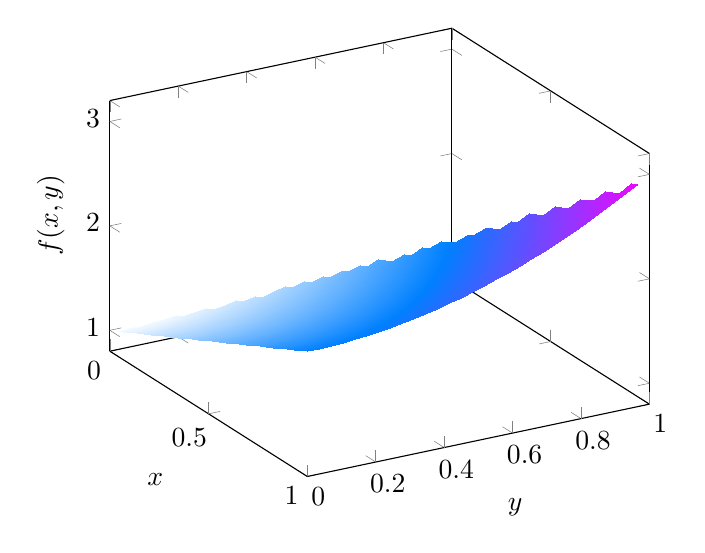
\begin{tikzpicture}
        \begin{axis}[
            view={60}{30},
            xlabel=$x$,
            ylabel=$y$,
            zlabel={$f(x,y)$},
            domain=0:1,
            y domain=0:1,
            samples=30,
            samples y=30,
            colormap/cool,
        ]
            \addplot3 [
                surf,
                domain=0:1,
                y domain=0:1,
                samples=30,
                samples y=30,
                restrict z to domain=-10:10,
                shader=interp,
            ]
            {y <= sqrt(x) ? 1 + x + y^2 : NaN};
        \end{axis}
    \end{tikzpicture}
\end{center}

First we are going to imagine slicing the area under this sector vertically along the \(x\)-axis from 
\(0\) up to \(1\) which is the volume of an Area under a curve that is represented by going along the 
\(y\)-axis.

\begin{align*}
    \int_{0}^{1}\int_{0}^{\sqrt{x}} 1 + x + y^2 dy dx \\
    \int_{0}^{1} \left| y + xy + \frac{y^3}{3} \right|_{0}^{\sqrt{x}} dx \\
    \int_{0}^{1} \left| \sqrt{x} + x\sqrt{x} + \frac{\sqrt{x}^3}{3} \right|_{0}^{\sqrt{x}} dx \\
    = \left| \frac{2}{3} x^{\frac{3}{2}} + \frac{4}{3} \frac{2}{5} x^{\frac{5}{2}} \right|_{0}^{1} = \frac{6}{5}
\end{align*}

If we choose the other way then we have an area with a fix \(y\) in the inside that goes from \(y^2\) to 
1 with respect to \(x\).

\[
    \int_{0}^{1}\int_{y^2}^{1} 1 + x + y^2 dx dy
\]

\subsection{Changing the order of integration to solve tricky integrals}

Given \(\int_{0}^{8}\int_{\sqrt[3]{x}}^{2} \frac{1}{y^4 +1}dy dx\) which is very hard to integrate, 
let us change the order to make it easier.

\[
    \int_{0}^{2}\int_{0}^{y^3} \frac{1}{y^4 +1}dx dy
\]

The steps are the same as in the previous Example.

\begin{enumerate}

    \item Identify the area you want to integrate, what are the bounds respective to \(x\) and \(y\)

    \item Write the same expression without bounds and change the order of the differentials

    \item Imagine slicing the area underneath vertically for \(x\) and horizontally for \(y\) with their 
          respective bounds corresponding to the perspective.

    \item Write the new integral with the opposite of order of integration

\end{enumerate}

\begin{center}

    Visualization of the area underneath the surface
    \smallskip

    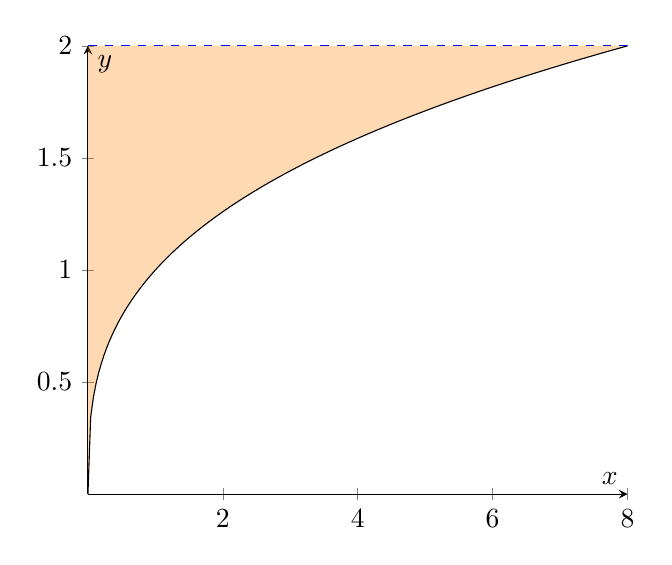
\begin{tikzpicture}
        \begin{axis}[
            axis lines=middle,
            xlabel={$x$},
            ylabel={$y$},
            legend pos=outer north east,
            domain=0:8,
            samples=200
        ]
            % Shading the area between the two functions
            \addplot [
                name path=A,
                domain=0:8,
                samples=200,
                draw=none
            ] {pow(x, 1/3)};
            
            \addplot [
                name path=B,
                domain=0:8,
                samples=200,
                draw=none
            ] {2};

            \addplot [
                orange,
                fill opacity=0.3
            ] fill between[of=A and B];

            \addplot[color=black, domain=0:8, samples=200]{pow(x, 1/3)};

            \addplot[color=blue, dashed, domain=0:8, samples=200]{2};

        \end{axis}
    \end{tikzpicture}
\end{center}

Here the original bounds are: \(x\) goes from 0 to 8 and \(y\) goes from \(\sqrt[3]{x}\) to 2.
As you can see in the diagram by slicing vertically the value of \(x\) is fixed, and we move 
towards the upper-bound of \(y\) which is 2.
Therefore, the smallest \(x\) can get is 0 and the biggest is 2. While for \(y\) by slicing 
vertically we get that \(x\) goes from 0 to \(\sqrt[3]{x}\), but 
we do not want to leave \(x\), so we solve for \(y\) and get \(y^3\). 
Now we can put all of this together and integrate.

In general changing the order of integration is only about using the logic to set the bounds of integration, 
but starting from a different perspective.

\subsection{The Jacobian}

The Jacobian matrix is a fundamental concept in multi-variable calculus. The Jacobian is the best
approximation of a linear transformation for a point.

For the intuition of why, we use partial derivatives, just think about
how we use them as this tiny changes in the component of original
basis vectors.

Given a vector-valued function

\[
    f : \Reals^n \rightarrow \Reals^m, \quad f(x_1, \ldots, x_n) = 
    \begin{bmatrix}
    f_1(x_1, \ldots, x_n) \\
    f_2(x_1, \ldots, x_n) \\
    \vdots \\
    f_m(x_1, \ldots, x_n)
    \end{bmatrix},
\]

the \emph{Jacobian matrix} of \(f\) is the \(m \times n\) matrix of all first-order partial derivatives:

\[
    J_f(x) = 
    \begin{bmatrix}
    \frac{\partial f_1}{\partial x_1} & \frac{\partial f_1}{\partial x_2} & \cdots & \frac{\partial f_1}{\partial x_n} \\
    \frac{\partial f_2}{\partial x_1} & \frac{\partial f_2}{\partial x_2} & \cdots & \frac{\partial f_2}{\partial x_n} \\
    \vdots & \vdots & \ddots & \vdots \\
    \frac{\partial f_m}{\partial x_1} & \frac{\partial f_m}{\partial x_2} & \cdots & \frac{\partial f_m}{\partial x_n}
    \end{bmatrix}.
\]

\subsubsection{Local linearity}

While performing non-linear transformations on a space. We can see that in a tiny neighborhood
around a point, the transformation appears to be linear. And the matrix that encodes that
transformation is the \emph{Jacobian}.

For intuition, just imagine that in the tiny neighborhood the transformation is composed
of small steps in the \(x_1, \dots, x_n\) directions which give of the partial derivatives that
represent this small steps. 

\subsubsection{Determinant}
When \(m = n\), i.e., the function maps from \(\Reals^n\) to \(\Reals^n\), the Jacobian matrix is square. 
In this case, the \emph{Jacobian determinant} is defined as:

\[
    \det(J_{f}(x)),
\]

and provides important information about the local behavior of the function. For instance:

\begin{itemize}

    \item If \(\det(J_{f}(x)) \neq 0\), the function is locally invertible at \(x\) by the inverse 
      function theorem.
  
      \item The sign and magnitude of the determinant 
      gives us information about orientation and volume scaling of the transformation.

\end{itemize}

When we change our systems of coordinates it is important that our differential make sense in the original 
system we were. Because of that, we take the determinant with respect to the new coordinates to tell us 
the scaling factor that we have to use for our result to make sense.

\textbf{Use Cases:}

The Jacobian matrix and its determinant appear in many areas, including:

\begin{itemize}
  
    \item \textbf{Change of variables in integrals:} The absolute value of the Jacobian determinant is 
          used to adjust the measure when changing coordinates in multiple integrals.
  
    \item \textbf{Nonlinear optimization:} The Jacobian is crucial for computing gradients and 
          performing techniques like Newton's method in multiple dimensions.
  
    \item \textbf{Differential equations:} Stability analysis of dynamical systems often involves 
          evaluating the Jacobian at equilibrium points.

\end{itemize}

\subsubsection{List of Common Jacobians}

\begin{itemize}

    \item \emph{Cartesian Coordinates}:

    \begin{itemize}
        
        \item Definition: The position of a point is given by \((x, y, z)\) in a 3D space along 
              orthogonal axes.
        
        \item Jacobian: 
        
            \[
                J_{\text{Cartesian}} = 1dx
            \]
    
    \end{itemize}

    \item \emph{Polar Coordinates (2D)}:

    \begin{itemize}

        \item Definition: The position of a point in a plane is given by \((r, \theta)\), where \(r\) 
              is the radial distance and \(\theta\) is the angle from the positive \(x\)-axis.
        
        \item Jacobian:
        
        \[
            J_{\text{Polar}} = rd rd\theta
        \]

    \end{itemize}

    \item \emph{Cylindrical Coordinates}:

    \begin{itemize}
        
        \item Definition: The position of a point in 3D space is given by \((r, \theta, z)\), where 
              \((r, \theta)\) are the polar coordinates in the \(xy\)-plane and \(z\) is the height along 
              the \(z\)-axis.
        
        \item Jacobian:
        
            \[
                J_{\text{Cylindrical}} = r\ dr d\theta dz
            \]

    \end{itemize}

    \item \emph{Spherical Coordinates}:
    
    \begin{itemize}
        
        \item Definition: The position of a point in 3D space is given by \((\rho, \theta, \phi)\), where:
        
        \begin{itemize}
            
            \item \(\rho\) is the distance from the origin,
            
            \item \(\theta\) is the azimuthal angle (in the \(xy\)-plane from the positive \(x\)-axis),
            
            \item \(\phi\) is the polar angle (from the positive \(z\)-axis).
        
        \end{itemize}
        
        \item Jacobian:
               
              \[
                    J_{\text{Spherical}} = \rho^2 \sin (\phi) d\rho d\theta d\phi
              \]
            
    \end{itemize}

\end{itemize}

\subsection{Integration in Polar Coordinates}

For radially symmetric regions or functions, switching to polar coordinates simplifies the computation.

\emph{Transformation:}

\[
    x = r \cos \varphi, \quad y = r \sin \varphi
\]

The Jacobian of the transformation gives the area element:

\[
    dA = r\, dr\, d\varphi
\]

\emph{Integral:}

\[
    \iint_D f(x, y)\, dA = \int_{\varphi_0}^{\varphi_1} \int_{0}^{R(\varphi)} f(r \cos \varphi, r 
    \sin \varphi)\, r\, dr\, d\varphi
\]

\subsubsection{Origin of the Area}

When we divide our circle in the sections we get both a difference in then angle and the radius which 
generate another area. The difference \(\Delta A =\) Area of big wedge \(-\) Area of small wedge

\emph{Radius: }\(r_k + \frac{\Delta r}{2}\) for the big wedge and \(r_k - \frac{\Delta r}{2}\) for the 
small wedge

\emph{Angle: }\(\frac{\Delta \theta}{2 \pi}\) which is the angle of the fraction of the circle 
because the formula for the area is \(r^2 \pi\) and the whole circle would be \(2\pi\)

\emph{Final Formula for the difference in the Area}

\[
    \Delta A = \frac{\Delta \theta}{2 \pi} \left ( {\left[r_k + \frac{\Delta r}{2}\right]}^2 - 
    {\left[r_k - \frac{\Delta r}{2}\right]}^2\right)
\] 

\[ 
    = r_k \Delta r \Delta \theta
\]

Which multiplied by the function value and by taking the limit of these sections we get that the volume:

\[
    V = \int_{\theta_1}^{\theta_2} \int_{r_1 (\theta)}^{r_2 (\theta)} f(r, \theta) r \Delta r \Delta 
    \theta
\]

\textbf{Example:}

\(f(r, \theta) = r\) above cardioid \(r = 1 - \sin \theta\)

Then

\[
    V = \int_{0}^{2\pi}\int_{0}^{1 - \sin \theta} r r dr d\theta
\]

\[
    = \int_{0}^{2\pi}\frac{r^3}{3} |_{0}^{1 - \sin \theta} d\theta = \int_{0}^{2\pi} 
    \frac{{(1 - \sin\theta)}^3}{3} d\theta = \frac{5 \pi}{3}
\]

\subsection{Improper Integrals over Unbounded Regions}

If the domain of integration is unbounded (e.g., the entire plane \( \Reals^2 \)), the double integral is 
defined via a limit process:

\[
    \iint_{\Reals^2} f(x, y)\, dx\, dy := \lim_{M_1, M_2 \to \infty} \lim_{N_1, N_2 \to \infty}
    \int_{M_1}^{M_2} \int_{N_1}^{N_2} f(x, y)\, dy\, dx
\]

Often, using polar coordinates simplifies such cases, reducing multiple limits to one:

\[
    \iint_{\Reals^2} f(x, y)\, dx\, dy = \int_0^{2\pi} \int_0^{\infty} f(r \cos \varphi, r \sin \varphi)\, 
    r\, dr\, d\varphi
\]

\subsubsection{Gaussian Integral}

We are going to find the integral of the \emph{unbounded integral} 
\(e^{-x^2}\)using a combination of techniques.

\begin{align*}
    S &= \int_{-\infty}^{\infty} e^{-x^2}dx\\
    S^2 &= \left(\int_{-\infty}^{\infty} e^{-x^2}dx\right) \left(\int_{-\infty}^{\infty} e^{-x^2}dx\right)\\
    S^2 &= \left(\int_{-\infty}^{\infty} e^{-x^2}dx\right) \left(\int_{-\infty}^{\infty} e^{-y^2}dy\right)
\end{align*}

Now let us translate to polar coordinates

\begin{align*}
    S^2 &= \left(\int_{0}^{2\pi} \int_{0}^{\infty}re^{-{(r\cos\theta)}^2} re^{-{(r\sin\theta)}^2}drd\theta\right)\\
    S^2 &= \left(\int_{0}^{2\pi} \int_{0}^{\infty}re^{-{(r\cos\theta)}^2 + {(r\sin\theta)}^2}drd\theta\right)\\
    S^2 &= \left(\int_{0}^{2\pi} \int_{0}^{\infty}re^{-(r^2)}drd\theta\right)\\
    S^2 &=  \left(\int_{0}^{2\pi} \int_{0}^{\infty}\frac{1}{2}e^{-(s)}dsd\theta\right)\\
    S^2 &= \left(\int_{0}^{2\pi}d\theta\right)\\
    S^2 &= \pi\\
    S   &= \sqrt{\pi}
\end{align*}

\QED

\subsection{Triple Integrals}

The triple integral allows the computation of volume or mass in three-dimensional space.

Let \( V \subset \Reals^3 \) be a bounded region, then:

\[
    \iiint_V f(x, y, z)\, dV = \lim_{n \to \infty} \sum_{k=1}^n f(x_k, y_k, z_k) \, \Delta V_k,
\]

where \( \Delta V_k \) are small sub-volumes approximating \( V \).

In practice, evaluate:

\[
    \iiint_V f(x, y, z)\, dz\, dy\, dx,
\]

with limits determined by the geometry of the volume. The order of integration may be rearranged to 
simplify computation.

\[
    \int_{x=a}^{x=b}\int_{y=g_1(x)}^{y=g_2(x)} \int_{f_1(x,y)}^{f_2(x,y)} dz dy dx
\]

\subsubsection{Triple Integrals in Cartesian Coordinates}

In this short section we, will look at an example of how to calculate the volume enclose in
between two functions using triple integrals.

Given are the functions \(f_1(x,y) = x^2 + y^2\) and \(f_2(x,y) = 3 - x^2 - y^2\)

\begin{center}
    
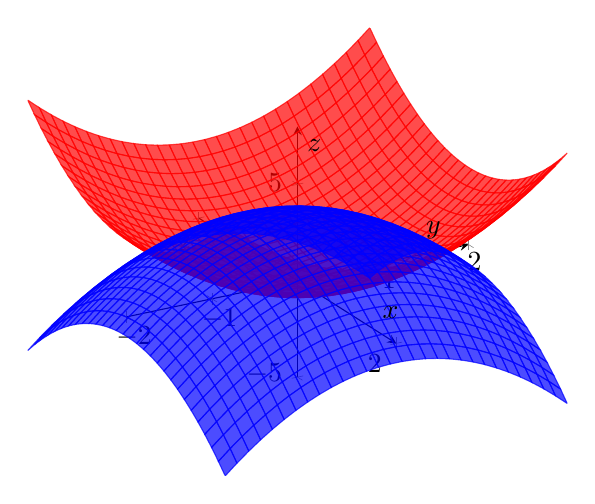
\begin{tikzpicture}
    \centering
    \begin{axis}[
        view={60}{30},
        axis lines=center,
        xlabel=$x$, ylabel=$y$, zlabel=$z$,
        domain=-2:2,
        y domain=-2:2,
        samples=30,
        samples y=30,
        colormap/jet,
    ]
        % Plot f1(x,y) = x^2 + y^2 in red
        \addplot3[
            surf,
            shader=flat,
            draw=red,
            fill=red,
            opacity=0.7,
        ]
        {x^2 + y^2};
    
        % Plot f2(x,y) = 3 - x^2 - y^2 in blue
        \addplot3[
            surf,
            shader=flat,
            draw=blue,
            fill=blue,
            opacity=0.7,
        ]
        {3 - x^2 - y^2};
    \end{axis}
\end{tikzpicture}
\end{center}

Let us find the intersection

\[
    x^2 + y^2 = 3 -x^2 - y^2 
\]
\[
    x^2 + y^2 = \frac{3}{2}
\]

Now we have to find the limits of integration for 

\[
    \int_{x=a}^{x=b}\int_{y=g_1(x)}^{y=g_2(x)} \int_{f_1(x,y)}^{f_2(x,y)} dz dy dx,
\]

using our constraint and our original functions.

\[
    \int_{x=a}^{x=b}\int_{y=-\sqrt{\frac{3}{2} - x^2}}^{\sqrt{\frac{3}{2} -x^2}} 
    \int_{x^2 + y^3}^{3-x^2-y^2} dz dy dx
\]

Here \(z\) means the height which is just the output
of the original functions.

The bounds of \(y\) just by looking at out constraint and solving for it.
And \(x\) only depends on the concrete limit of integration.

\subsubsection{Coordinate Transformation and the Jacobian Determinant}

Let a coordinate transformation be defined by:

\[
    x = x(u, v, w), \quad y = y(u, v, w), \quad z = z(u, v, w)
\]

Then the triple integral transforms as:

\[
    \iiint_{(x, y, z)} f(x, y, z)\, dx\, dy\, dz = \iiint_{(u, v, w)} f(x(u, v, w), y(u, v, w), 
    z(u, v, w)) \cdot \left| \det J \right|\, du\, dv\, dw
\]

where \( J \) is the \emph{Jacobian matrix} of the transformation:

\[
    J = 
    \begin{bmatrix}
    \frac{\partial x}{\partial u} & \frac{\partial x}{\partial v} & \frac{\partial x}{\partial w} \\
    \frac{\partial y}{\partial u} & \frac{\partial y}{\partial v} & \frac{\partial y}{\partial w} \\
    \frac{\partial z}{\partial u} & \frac{\partial z}{\partial v} & \frac{\partial z}{\partial w}
    \end{bmatrix}
\]

\textbf{Example: Transformation to Cylindrical Coordinates}

The standard cylindrical coordinate transformation is:

\[
    x = r \cos \varphi, \quad y = r \sin \varphi, \quad z = z
\]

The Jacobian determinant is:

\[
    \left| \det J \right| =
    \begin{vmatrix}
    \cos \varphi & -r \sin \varphi & 0 \\
    \sin \varphi & r \cos \varphi & 0 \\
    0 & 0 & 1
    \end{vmatrix}
    = r
\]

Thus, the triple integral in cylindrical coordinates becomes:

\[
    \iiint f(x, y, z)\, dx\, dy\, dz = \iiint f(r \cos \varphi, r \sin \varphi, z)\, r\, dr\, d\varphi\, 
    dz
\]

\subsubsection{Calculating the center of mass with triple integrals}

We can make use of triple integration to calculate the center of mass of a body with
respect to \(x\), \(y\) or \(z\) with the following formulas:

\begin{align*}
    x_s &= \iiint_V xp(x,z,y)dz\ dy \ dx\\
    y_s &= \iiint_V yp(x,z,y)dz\ dy \ dx\\
    z_s &= \iiint_V zp(x,z,y)dz\ dy \ dx
\end{align*}

Where \(p(x,y,z)\) is our mass function.

\newpage
\section{Differential Equations}

A Differential Equation is an equation that relates a function (the dependent variable)
with a variable or multiple variables (the independent variables) and its derivative.

They can be categorized in \emph{Ordinary} and \emph{Partial} Differential Equations.

\subsection{Ordinary Differential Equations}

An equation of the form

\[
    y^n = f(x, y, x', y', \dots, y^{n -1})
\]

is called \emph{Ordinary Explicit Differential Equations of order} \(n\)

If \(y^n = 0\) then it is \emph{implicit}

If the exponent of the dependent variable is 1, and it
is build like a linear equation then it is categorized as \emph{Linear}

\subsection{Initial Value Problems and Solutions}

The specification of an explicit differential equation and the values

\[
    x_0,\quad y(x_0) = y_0,\quad y'(x_0) = y_1,\quad \dots,\quad y^{(n-1)}(x_0) = y_{n-1}
\]

is called an \emph{initial value problem (IVP)}.

An \(n\)-times differentiable function \( y(x) \) that satisfies
the explicit differential equation is called the \emph{general solution} of the
differential equation. If it also satisfies the conditions of the initial value problem
from the previous definition, it is called the \emph{particular solution} of the IVP\@.

\subsection{Volterra Integral}

The function \(y(x)\) is a solution of the IVP \(y' = f(x,y),\quad y(x_0) = y_0\) if and only if

\[
    y(x) = y_0 + \int_{x_0}^{x} f(t, y(t))dt
\]

\textbf{Proof:}

\[
    \int_{x_0}^{x} f(t, y(t))dt = \int_{x_0}^{x} y'
\]
\[
    y(x) = y(x_0)
\]

The other way would be

\[
    \left(\int_{x_0}^{x} f(t, y(t))dt + y_0\right)' = f(x, y(x)) = y'
\]

\QED

\subsection{The Picard-Lindelöf Iteration Method}

We can approximate the desired solution using the Volterra integral equation as follows.
Start with an arbitrary initial function, for example a constant — preferably the initial value:

\[
    g_0(x) = y_0
\]

Then form the next approximation to the desired function \( y(x) \) as:

\[
    g_{n+1}(x) = y_0 + \int_{x_0}^{x} f(t, g_n(t)) \, dt
\]

\subsection{Integration case}

To solve a ODE of the form \(y' = f(x)\) it is as easy as integrating \(f(x)\).

\subsection{Separation of Variables}

An equation \(F(x,y,y',\dots) = 0\) is a called an equation of \emph{separable variables} if it can
be written in one of the following forms:

\begin{itemize}

    \item \(\frac{dy}{dx} = f(x) g(y)\)

    \item \(\frac{dy}{dx} = \frac{f(x)}{g(y)}\)

    \item \(\frac{dy}{dx} = \frac{g(y)}{f(x)}\)

\end{itemize}

\subsubsection{Steps to solve a ODE of separable variables}

\begin{enumerate}

    \item Solve for the derivative

    \item Check that it is indeed an ODE of separable variables

    \item Separate the variables

    \item Integrate with respect to the independent variable

\end{enumerate}

\textbf{Example:}

Given is \((y - 2)y' = 3x - 5\)

It is an ODE of separable variable

\[
    y' = \frac{3x - 5}{y - 2}
\]

Now we separate the variables and Integrate

\[
    \int (y - 2)y' dx = \int 3x - 5 dx
\]

Note that \(y' = \frac{dy}{dx}\) and \( \frac{dy}{dx} dx = dy\) (only as a convenient fiction
in reality we are changing the variables) thus,

\[
    \int (y - 2)dy = \int 3x - 5 dx
\]

\[
    \frac{y^2}{2} - 2y + c = \frac{3x^2}{2} - 5x + c
\]

The solution we get is an implicit solution. To make it look nice solve for \(y\)
if you can.

\subsubsection{Understanding the fiction}

The previous fiction we used can explain in the following manner.

Given \( f(y) \frac{dy}{dx} dx = \int f(y) dy\). We want to prove that this equality holds via the
\emph{chain rule} \(\frac{du}{dx} = \frac{du}{dy} \frac{dy}{dx}\).

\begin{align*}
    \frac{d}{dx} \left( \int f(y) dy \right) & = \frac{d}{dx} \left( \int f(y) dy \right) \frac{dy}{dx} \\
                                             & = f(y) dy \frac{dy}{dx}                                  \\
                                             & \implies \int f(y) \frac{dy}{dx} = \int f(y) dy
\end{align*}
\QED

\subsection{Geometry of ODE}

You can imagine the plot of an ODE as a \emph{Slope field} where the slope (derivative) of a function
obeys a certain condition, this being the differential equation \(\frac{dy}{dx} = expr\).

A point on this field is called an \emph{Initial Condition} and the curve that goes through
that point in the slope field is called an \emph{Integral curve} which a solution to the differential
equation with respect to that initial condition.

\subsection{Existence and Uniqueness}

Let \( f(x, y) \) be continuous on a rectangle \( [a, b] \times \Reals \). Then the differential
equation

\[
    y' = f(x, y)
\]

has at least one solution. A unique solution is only guaranteed under additional conditions.

A function \( f : \Reals^2 \to \Reals \) is called
\emph{Lipschitz continuous with respect to \(y\)} if there exists a constant \( L > 0 \) such that

\[
    |f(x, y_1) - f(x, y_2)| \leq L |y_1 - y_2|
    \quad \text{for all } (x, y_1), (x, y_2) \in D.
\]

Let \( x_0 \in [a, b] \), and let \( f : [a, b] \times \Reals \to \Reals \) be continuous
and bounded, and Lipschitz continuous in \(y\). Then the initial value problem

\[
    y' = f(x, y), \quad y(x_0) = y_0
\]

has a unique solution on \( [a, b] \).

Or in easier words: If \(f\) and \(\frac{\partial f}{\partial y}\) are continuous near \((x_0, y_0)\)
then there is a unique solution on an interval \(\alpha < x_0 < \beta\) to the IVP

\[
    y' = f(x,y), \quad y(x_0) = y_0
\]

\subsection{How to deal with initial conditions}

After solving a differential equation we may have the problem that certain initial
conditions were set at the start, thus, making our general solution not specific.

Solving this problem is pretty easy, because we just have to solve for the constant terms
in our general solution with respect to our initial conditions. Like for example \(y(0) = 1\)
we would plug 0 for all \(x\)'s in our general solution the whole equation will be set equal to 1.

\subsection{Solving DE with Substitution}

In some cases a complex function can be simplified via a substitution.

\subsubsection{Case I}

\[
    y' = f(ax + by(x) + c)
\]

With a substitution like \(z(x) = ax + by(x) + c\) the right-hand side will become \(f(z)\)
and for the left-hand side we get \(y(x) = \frac{z(x) - ax - c}{b}\).

Now we can substitute in the original equation, and we get

\[
    y'(x) = \frac{1}{b} (z'(x) - a) = f(z)
\]

\[
    z'(x) = a + b f(z)
\]

Now we can integrate and find the solution and then return to our original variables.

\textbf{Example:}

\[
    y' = (x + y(x))^2
\]

Here \(a = 1\), \(b = 1\), \(c = 0\) and \(f(z) = z^2\)

\textbf{1. Substitute}

\[
    z(x) = x + y(x)
\]
\[
    y(x) = z(x) - x
\]
\[
    y'(x) = z'(x) - 1
\]

\textbf{2. Plug in the DE}

\[
    y' = {(x + y(x))}^2
\]
\[
    z'(x) - 1 = {z(x)}^2
\]

\textbf{3. Integrate}

\[
    z'(x) = 1 + {z(x)}^2
\]
\[
    \frac{z'(x)}{1 + {z(x)}^2}
\]
\[
    \int \frac{1}{1 + z^2} dz = \int 1 dx
\]
\[
    \arctan (z) = x + c
\]
\[
    z = \tan(x + c)
\]

\textbf{4. Return to the original variables}

\[
    x + y(x) = \tan(x + c)
\]
\[
    y(x) = \tan(x + c) - x
\]

\subsubsection{Case II}

\[
    y' = f(\frac{y}{x})
\]

For this to be valid \(z(x) = \frac{y}{x}\) our \(y(x)\) needs to look like \(y(x) = z(x)x\)
and so \(y' = z(x) + z'(x)x\).

Now we substitute in the differential equation using \(f(z) = z(x) + z'(x)x\)

\[
    z'(x) = \frac{f(z) - z(x)}{x}
\]

Now we can integrate and then return to our original variables. \(y(x) = z(x)x \), where \(z(x)\) is our
result of the integration.

\textbf{Example:}

\[
    y' = \frac{y(x)}{x} + 1
\]

This in converted to \(y' = f(z) = z + 1\)

\textbf{1. Substitute}

\[
    z(x) = \frac{y(x)}{x}
\]
\[
    y(x) = z(x)x
\]
\[
    y'(x) = z(x) + z'(x)x
\]

\textbf{2. Plug in the DE}

\[
    z(x) + z'(x)x = z(x) + 1
\]

\textbf{3. Integrate}

\[
    z'(x)x = 1
\]
\[
    \int z' dz = \int \frac{1}{x} dx
\]
\[
    z = (\ln(x) + c)x
\]

\subsection{Linear Differential Equations}

An ODE is called linear if all occurrences of the dependent variable and its
derivatives have an exponent of at most 1.

\[
    a_n(x)y^n + a_{n - 1}y^{n -1} + \cdots + a_1(x)y' + a_0(x)y = b(x)
\]

If such an Equation has also the property \(b(x) = 0\) it is called \emph{Homogeneous}

\subsubsection{How to solve a Linear Differential Equation}

In this case we will focus on first Order ODE.

Write it in the standard form \(y' + p(x)y = f(x)\)

Now use \emph{Integrating Factor Method}

\subsection{Integrating Factor Method}

We are going to multiply our expression by function \(r(x)\)

\[
    r(x)y' + r(x)p(x)y = r(x)f(x)
\]

Now we would like to write the left side as \(\frac{d}{dx} y r(x)\) because now if we
were to integrate it would take us to the expression in the right.

When we evaluate this new expression we get that

\[
    \frac{d}{dx} y r(x) = y'r(x) + r'(x)y
\]

which is not quite what we actually have, but it is close. Now note that we can say

\[
    r'(x) = r(x)p(x)
\]

This is a differential equation of separable variables thus, we can

\[
    \frac{r'(x)}{r(x)} = p(x)
\]

\[
    \int \frac{r'(x)}{r(x)}dx = \int p(x)dx
\]

\[
    \ln(r(x)) = \int p(x) dx
\]

after using \(e\)

\[
    r(x) = e^{\int p(x) dx}
\]

Now we have found an \(r(x)\) and now that we know that such a function exists we can return
to our initial problem and say

\[
    \frac{d}{dx}r(x)y = r(x)f(x)
\]

\[
    y = \frac{1}{r (x) } \int r (x) f (x) dx
\]

and

\[
    r(x) = e^{\int p (x) dx}
\]

To summarize, given \(y' + f(x)y = g(x)\) the steps are:

\begin{enumerate}

    \item Find \(c(x) = e^{\int f(x)dx}\).

    \item Multiply the original expression with \(c(x)\).

          \[
              y'c(x) + f(x)c(x)y = g(x)c(x)
          \]

    \item Use the power rule of differentiation to simplify.

          \[
              y'c(x) + f(x)c(x)y = \frac{d}{dx}\left(c(x), y\right)
          \]

    \item Integrate.

          \begin{align*}
              \int \frac{d}{dx}\left(c(x), y\right)dx & = \int g(x)c(x)dx              \\
              c(x)y                                   & = \int g(x)c(x)dx              \\
              y                                       & = \frac{\int g(x)c(x)dx}{c(x)}
          \end{align*}

\end{enumerate}

\textbf{Example:}

Given are \(y' + 4y = e^{-x}\) and \(y(0) = \frac{4}{3}\).

Here \(4 = p(x)\) and \(e^{-x} = f(x)\).

Now let us use the formula for \(r(x) = e^{\int p (x)}\). This gives us
\(r(x) = e^{\int 4dx} = e^{4x}\).

Now recall what we saw earlier

\[
    e^{4x}y' + e^{4x}4y = e^{4x}e^{-x} = e^{3x}
\]

Our left side is just \(\frac{d}{dx} e^{4x}y\)

Now let us complete the exercise with our last formula by integrating both sides

\[
    \frac{d}{dx} e^{4x}y = e^{3x}
\]
\[
    y = \frac{1}{e^4x}\int e^{3x}
\]
\[
    y = \frac{1}{e^4x} \frac{1}{3}e^{3x} + c
\]

Which is our general solution

To find our specific solution we just plug 0 in to our general solution that gives us
\(\frac{1}{3} + c = \frac{4}{3}\) thus, \(c = 1\)

\subsection{Homogeneous Differential Equations}

A differential equation

\[
    M(x,y)dx + N(x,y)dy = 0
\]

is considered \emph{Homogeneous} if and only if
\(M(x)\) and \(N(x)\) are \emph{homogeneous}, and they have the same degree.

The equation \(y' + f(x)y = 0\) is called \emph{homogeneous linear differential equation of first order}.

\subsubsection{Homogeneous Equation}

A function \(f(x,y)\) is called \emph{homogeneous} if and only if it can be written

\[
    f(xt, yt) = t^n f(x,y)
\]

\textbf{Example: }

\[
    f(x,y) = x^3 + y^3
\]
\[
    f(tx, ty) = {(tx)}^3 + {(ty)}^3
\]
\[
    t^3 (x^3 + y^3) = t^3 f(x,y)
\]

It is important to note that the key is that each term have a total degree of \(n\).
For example: \(x^2y + x3y^2\)

\subsubsection{Homogeneous Functions Theorem}

If \(f(x,y)\) is homogeneous of degree \(0\) in \(x\) and \(y\) then
\(f\) is a function of \(\frac{y}{x}\)

Or \(f(x,y,y')\) is homogeneous if it can be written as \(y' = f(\frac{x}{y})\) or \(y' = f(\frac{y}{x})\)

\subsection{Solving Homogeneous DE I}

\begin{enumerate}
    \item Write in the form \(M(x,y)dx + N(x,y)dy = 0\)
    \item Check if it is homogeneous
    \item Change the variables to \(y = ux\) or \(x = uy\) depending on the situation
    \item Solve using the method of separable variables method
    \item Rewrite the answer in terms of the original variables again
\end{enumerate}

\textbf{Example:}

Give is the function \((x -y)dx = - xdy\)

\textbf{Step 1.} We write it in the desired form \((x - y)dx + xdy = 0\)

\textbf{Step 2.} We notice that both are of degree \(1\). This time we skip the rigorous check.

\textbf{Step 3.} We are going to choose the simpler function to do the change of variable
depending on the \emph{differential!}

The simpler function is \(xdy\) thus, we are to change \(y\)

\[
    y = ux
\]
\[
    dy = ux' + xu'
\]

and

\[
    u = \frac{y}{x}
\]

Now substitute

\begin{align*}
    (x - ux)dx + x(udx + xdu)       & = 0         \\
    xdx - u x dx + x u dx + x^{2}du & = 0         \\
    (x - ux + xu)dx + x^{2}du       & = 0         \\
    xdx + x^{2}du                   & = 0         \\
    xdx                             & = - x^{2}du \\
    dx                              & = - xdu
\end{align*}

\textbf{Step 4.} Now we can integrate both sides

\[
    \int \frac{1}{x}dx = \int du
\]
\[
    \ln x + c = -u + c
\]

\textbf{Step 5.} No we use \(u = \frac{y}{x}\) to return to our original variables

\[
    \ln x + c = -\frac{y}{x} + c
\]
\[
    -x\ln x - xc = y
\]

\subsection{Solving Homogeneous DE I}

Another method for solving this kind of equations \(y' + f(x)y = 0\)is to follow the next steps.

\textbf{Step 1: Separate the variables}

\[
    \frac{dy}{dx} = -f(x)y
\]

\textbf{Step 2: Use the separation of variables}

\[
    \int \frac{\frac{dy}{dx}}{y} = \int -f(x) dx
\]

\[
    \int \frac{dy}{y} = \int -f(x) dx
\]

\[
    \ln|y| = \int -f(x) dx
\]

\[
    y = C e^{\int -f(x) dx}
\]

This method works more directly.

\subsection{Inhomogeneous Equation}

The equation \(y' + f(x)y = g(x)\) is called \emph{linear inhomogeneous differential equation
    of first order} \(g(x)\) is called the \emph{distortion function}. The correspondent IVP is called
\emph{linear} IVP\@.

\subsection{Solutions of LDE}

Every linear IVP with continuous functions \(f(x)\) and \(g(x)\) plus a bounded \(f(x)\)
has exactly one solution.

\textbf{Proof:}

\begin{align*}
    y' = -f(x)y + g(x) \text{ therefore, } |-f(x)y_1 + g(x) + -f(x)y_2 + g(x) | & = |f(x)||y_1 - y_2| \\
                                                                                & \le M |y_1 - y_2|
\end{align*}

Therefore, the function is Lipschitz continuous, thus, a solution is possible.
\QED

\subsubsection{Variation of the Constants}

Recall that for the homogeneous case \(y' + f(x)y = 0\) case we use
\(y = c e^{\int -f(x) dx}\), but now we have \(y' + f(x)y = g(x)\), thus, let us use the following
approach

\[
    y = c(x) e^{\int -f(x) dx}
\]

Now use the product rule to derivate

\begin{align*}
    y' & = c'(x) e^{\int -f(x) dx} + c(x)e^{\int -f(x) dx}(-f(x)) \\
       & = c'(x)e^{\int -f(x) dx} - f(x)y
\end{align*}

thus,

\[
    y' + f(x)y = c'(x)e^{\int -f(x) dx}
\]

therefore, \(g(x) = c'(x)e^{\int -f(x) dx}\)

Then we can get a solution for \(c(x)\) from

\[
    g(x) = c'(x)e^{\int -f(x) dx}
\]
\[
    g(x) = c'(x)e^{-\int f(x) dx}
\]
\[
    c'(x) = \frac{g(x)}{e^{-\int f(x) dx}}
\]
\[
    c'(x) = g(x)e^{\int f(x) dx}
\]

\textbf{Example: }

Given is \(y' -\cos(x)y = x e^{\sin(x)}\) with \(y(0) = 3\).

\textbf{1. Solve as if it were homogeneous}

\begin{align*}
    y' -\cos(x)y      & = 0              \\
    y'                & = \cos(x)y       \\
    \frac{y'}{y}      & = \cos(x)        \\
    \int\frac{1}{y}dy & = \int \cos(x)dx \\
    \ln |y| + c       & = \sin(x) + c    \\
    y                 & = e^{\sin(x)}c
\end{align*}

\textbf{2. Use \(y = c(x)e^{\sin(x)dx}\)}

\begin{align*}
    y'            & = c(x)\cos(x)e^{\sin(x)} + c'(x)e^{\sin(x)} \\
    y'            & = \cos(x)y + c'(x)e^{\sin(x)}               \\
    y' - \cos(x)y & = c'(x)e^{\sin(x)}
\end{align*}

\textbf{3. Compare with the original equation}

\begin{align*}
    y' -\cos(x)y  & = x e^{\sin(x)}    \\
    y' - \cos(x)y & = c'(x)e^{\sin(x)}
\end{align*}

\textbf{4. Solve for \(c'(x)\)}

\begin{align*}
    xe^{\sin(x)} & = c'(x)e^{\sin(x)} \\
    x            & = c'(x)
\end{align*}

\textbf{5. Integrate}

\begin{align*}
    \int x dx         & = \int c'(x)dx \\
    \frac{x^2}{2} + c & = c(x)
\end{align*}

\textbf{6. Substitute in our approach \(y = c(x)e^{\sin(x)}\) from earlier}

\[
    y = \left(\frac{x^2}{2} + c\right)e^{\sin(x)}
\]

\textbf{7. Solve for \(c\) using our initial condition if asked}

\[
    y(0) = 3
\]
\[
    3 = \left(\frac{0^2}{2} + c\right)e^{\sin(0)}
\]
\[
    3 = c
\]

\subsection{Existence and Uniqueness Differential Equations}

For the IVP

\[
    y^{n} + p_{n - 1}y^{n - 1}+ \cdots + p_0 (x)y = f(x)
\]

\[
    y(a) = b_0, y'(a) = b_1, \dots, y^{n - 1}(a) = b_{n - 1}
\]

If all \(p_i\) and \(f\) are continuous on the interval \(I\) about \(a\), then
there exists a unique solution on \(I\).

\subsection{Theorem of Superposition and the General Solution}

Suppose \(y_1, \dots, y_n\) solve

\[
    y^{n} + p_{n - 1}y^{n - 1}+ \cdots + p_0 (x)y = 0
\]

Then \(y = c_1 y_1 + \cdots + c_n y_n\) also solves the equation, and it is the
\emph{General Solution} if and only if the \emph{Wronskian} \(W(t) \ne 0\) for some \(t_0\).

\subsection{Undetermined Coefficients}

Given an equation \(y' + ay = g(x)\) notice that \(a\) does not depend on \(x\).
The homogeneous equation to this case will be \(y' + ay = 0\) with a solution \(y_h\) and some
partial solution \(y_p\). Now remember from \emph{Linear Algebra} the
\(general = particular + homogeneous\) more precisely \(y = y_p + y_h\) therefore, adding a
particular solution to a homogeneous does not change
the general solution of our DE.

Now let us substitute in our differential equation.

\begin{align*}
    (y_h + y_p)' + a(y_h + y_p) & = y_h' + y_p' + ay_h + ay_p                       \\
                                & = (y_h' + ay_h) + (y_p' + ay_p) = 0 + g(x) = g(x)
\end{align*}

\subsubsection{Steps for solving Constant Coefficients problems}

\begin{enumerate}

    \item Find the \emph{homogeneous} solution for \(y' + ay = 0\). \(y_h\) is going
          to have a free parameter.

    \item Find a partial solution for \(y' + ay = g(x)\)

    \item Use \(y = y_h + y_p\)

    \item If you have an IVP solve for the free parameter in \(y_h\)

\end{enumerate}

Now we have to find a way to solve for \(y_p\) and \(y_h\)

\subsubsection{Find the partial solution}

We will use the method called based on guessing the type of the function on the right side.

\textbf{Example: }

Given is the following IVP: \(y' + 2y = 2x + 13\) with \(y(0) = 8\)

By looking carefully we see that on the right-hand side we just have a normal polynomial,
thus, we can substitute \(y = bx + c\) and derivate \(y' = b\). In the case for when we have higher
order derivative we would differentiate for each of them.

Now substitute

\[
    b + 2(bx + c) = 2x + 13
\]

\[
    2bx + b + 2c = 2x + 13
\]

Now by comparing the Coefficients with the other side

\[
    2b = 2
\]
\[
    b + 2c = 13
\]

We get: \(b = 1\), \(c = 6\). And we have found a \emph{particular} solution for our DE
\(y_p = x + 6\)

Now we have to find a \emph{homogeneous} solution with the formula we already know
\(y_h = c e^{\int f(x)dx}\) in our case \(y_h = c e^{\int 2dx} = ce^{-2x}\)

\[
    y = y_h + y_p = c e^{-2x} + x + 6
\]

Now considering the condition \( y(0) = 8 \), this gives:

\[
    y(0) = c + 6 = 8 \Rightarrow c = 2
\]

and we obtain the particular solution:

\[
    y = 2 e^{-2x} + x + 6
\]

\subsubsection{Table of reference}
\bigskip
\begin{tabular}{|l|l|l|}
    \hline
    \textbf{Type of Forcing Function} & \textbf{Disturbance Function \( g(x) \)} &
    \textbf{Approach for \( y_p \)}                                                                                    \\
    \hline
    Constant                          & \( k_0 \)                                & \( c_0 \)                           \\
    \hline
    Linear                            & \( k_0 + k_1 x \)                        & \( c_0 + c_1 x \)                   \\
    \hline
    Polynomial                        & \( \sum\limits_{i=0}^{n} k_i x^i \)      & \( \sum\limits_{i=0}^{n} c_i x^i \) \\
    \hline
    Exponential                       & \( k e^{bx}, \; b \ne a \)               & \( c_0 e^{bx} \)                    \\
                                      & \( k e^{ax} \)                           & \( c_0 x e^{ax} \)                  \\
    \hline
    Trigonometric                     & \( k \sin(bx) + l \cos(bx) \)            & \( c_0 \sin(bx) + c_1 \cos(bx) \)   \\
    \hline
\end{tabular}

It is important to point out that sometimes it is necessary to combine different types
of functions to get the solution.

\textbf{Example:}

\[
    y'' -2x' 3y = t^2  + 3e^{-t} \cos (4t)
\]

Here the approach would be

\[
    y_p = (A + Bt + Ct^2) + D(e^{-t}\cos(4t)) + E(e^{-t}\sin(4t))
\]

The best way is to tackle down each of the types of functions separately.

An alternative to way of using this method is to

\begin{enumerate}

    \item Find the homogeneous solution.

    \item Multiply both sides of the equation by it.

    \item Integrate

\end{enumerate}

This will give you the exact same result and is faster.

\subsection{Bernoulli Equation}

This is used for equations of the form

\[
    y' + P(x)y = Q(x)y^n
\]

We can not use the methods we already know for this equation because it is linear but with a
clever substitution we can turn it into a linear differential equation.

Let us use a substitution

\[
    u = y^{1 - n}
\]

then

\[
    u' = (1 - n)y^{-n} y'
\]

Now this
looks kinda similar to the original equation multiply by \(y^{-n}\) that looks like

\[
    y^{-n}y' + P(x)y^{-n}y = Q(x)y^{-n}y{n}
\]

\[
    y^{-n}y' + P(x)y^{1 - n} = Q(x)
\]

Notice that \(y^{-n} = \frac{u'}{(1-n)y'}\), thus, after substitution

\[
    \frac{1}{1 - n}u' + P(x)u = Q(x)
\]

Now our equation is \emph{linear}, and we can use the \emph{integrating factor} method.

\textbf{Example: }

Given is \(y' -5y = \frac{-5}{2}xy^3\).

\[
    u = y^{-2}  \text{ and } u' = -2y^{-3}y'
\]

\[
    y^{-3} = \frac{u'}{-2y'}
\]

And our equation after multiplying by \(y^{-3}\)

\[
    y^{-3}y' - 5yy^{-3} = -\frac{5}{2}x
\]

\[
    y^{-3}y' - 5y^{-2} = -\frac{5}{2}x
\]

\[
    \frac{u'}{-2y'}y' - 5u = -\frac{5}{2}x
\]

Now we can use the \emph{Integrating Factor Method}. First bring to the standard form.
\(y' + p(x)y = f(x)\)

\[
    u' + 10u = 5x
\]

Remember that \(r(x) = e^{\int p(x)dx} = e^{\int 10 dx} = e^{10x}\) therefore, we have

\[
    e^{10x}u' + 10ue^{10x} = e^{10x}5x
\]

Now let us integrate

\[
    \frac{d}{dx} \left(e^{10x}u\right) = e^{10x}5x
\]

\[
    Ce^{10x}u = \int e^{10x} 5x dx = 5x \frac{e^{10x}}{10} - \int e^{10x}5dx
\]

\[
    Ce^{10x}u = \int e^{10x} 5x dx = 5x \frac{e^{10x}}{10} - \frac{5}{10}\int e^{10x}dx
\]

\[
    Ce^{10x}u = \frac{xe^{10x}}{2} - \frac{5}{100} e^{10x} + c
\]

\[
    Ce^{10x} = \frac{x}{2} - \frac{1}{20} + \frac{c}{e^{10x}} = y^{-2}
\]

\subsection{Autonomous Equations}

An \emph{Autonomous Differential Equation} only depends on the dependent
variable \(y\).\textbf{ Example: } \(\frac{dy}{dt} = (1 + y)(1 -y)\).

\subsubsection{Equilibrium Solutions}

Values where \(f(y) = 0\) are \emph{Equilibrium Solutions}.

\subsubsection*{Asymptotically stable}

An equilibrium solution \(y = a\) is \emph{asymptotically stable} if solutions
that start near \(a\) tend towards \(a\) as \(t \to \infty\).

\subsubsection*{Asymptotically unstable}

An equilibrium solution \(y = a\) is \emph{asymptotically unstable} if solutions
that start near \(a\) leave as \(t \to \infty\)

\subsection{Linear Inhomogeneous DEs with Non-Constant Coefficients}

The method of \emph{variation of constants} is often used alongside the \emph{superposition principle}.
In this method, the integration constant in the function \( c(x) \) is omitted as it is part of the
particular solution.

The superposition principle also holds for linear inhomogeneous differential equations with
non-constant coefficients:

\begin{align*}
    y_p' + f(x)y_p & = g(x) \quad \text{(particular solution)} \\
    y_h' + f(x)y_h & = 0 \quad \text{(homogeneous solution)}
\end{align*}

For the total solution \( y = y_h + y_p \), we get:

\begin{align*}
    y' + f(x)y
     & = (y_h + y_p)' + f(x)(y_h + y_p)  \\
     & = y_h' + y_p' + f(x)y_h + f(x)y_p \\
     & = g(x)
\end{align*}

Thus, the solution can be decomposed into the general solution of the homogeneous DE and a
particular solution based on the form of the right-hand side.

\textbf{Example: }

\[
    y' = -\frac{y}{x} + 1
\]

The homogeneous DE is \(y' = -\frac{y}{x}\) which can be solved by separating the variables.
\(y_h = \frac{c}{x}\)

Now let use \(y_p = \frac{c(x)}{x}\).

\[
    y_{p}' = \frac{c'(x)x - c(x)}{x^2}
\]

Let us break down the fraction to find where to put our homogeneous solution we have already found

\[
    \frac{c'(x)}{x} - \frac{c(x)}{x^2} = \frac{c'(x)}{x} + \frac{1}{x}\frac{c}{x}
    = \frac{c'(x)}{x} + \frac{1}{x}y
\]

and we get

\[
    y_{p}' = -\frac{y}{x} + \frac{c'(x)}{x}
\]

Here we compare with the inhomogeneous part of the original equation and get

\[
    \frac{c'(x)}{x} = 1 \implies c'(x) = x
\]

then \(c(x)\) is equal to \(\frac{x^2}{2}\) and therefore, \(y_p = \frac{x^2}{x}\frac{1}{x} =
\frac{x}{2}\)

As our final result we get \(y = \frac{c}{x} + \frac{x}{2}\)

\subsection{Power Series Approach}

Another method to solve a certain type  of differential equation
is to find the function given an initial conditions. This can be better understood with an example.

\[
    y' = y
\]
\[
    y(0) = 1
\]

We say \(y = \sum_{n = 0}^{\infty} a_n x^n\) and \(y(0) = a_0 = 1\).

Now let us derivate you \(y\)

\[
    y = \sum_{n = 0}^{\infty} a_n x^n = a_0 x^0 + a_1 x^1 + \cdots = 1 + a_1 x^1 + a_2 x^2 + \cdots
\]
\[
    y' = 0  + a_1 + 2 a_2 x + 3 a_3 x^2 + \cdots
\]

Thus, we can rewrite the sum as

\[
    y' = \sum_{n = 1}^{\infty} a_n n x^{n - 1}
\]

Starting from 1 because 0 does not contribute to the sum. After shifting the index we get

\[
    y' = \sum_{n = 0}^{\infty} a_{n + 1}(n + 1)x^{n}
\]

Now we build our original DE with our new definitions for \(y'\) and \(y\)

\[
    \sum_{n = 0}^{\infty} a_{n + 1}(n + 1)x^{n} = \sum_{n = 0}^{\infty} a_n x^n
\]

If we compare the coefficients we get

\[
    a_n = a_{n+1}(n+1)
\]

\[
    \frac{a_n}{(n + 1)} = a_{n+1}
\]

after iterating backwards we get

\[
    a_{n + 1} = \frac{a_n}{n + 1} = \frac{\frac{a_{n - 1}}{(n - 1 +1)}}{n + 1} =
    \frac{\frac{\frac{a_{n - 2}}{(n - 1)}}{(n - 1 + 1)}}{n + 1}
\]
\[
    a_n = \frac{a_0}{(n + 1)!} = \frac{1}{(n + 1)!} = 1
\]

therefore, \(a_n = \frac{1}{n!}\) which gives us the solution

\[
    \sum_{n = 0}^{\infty}\frac{1}{n!}x^n = e^x
\]

\subsubsection{Theorem for the Power Series of DE}

For a differential equation of the form:

\[
    A(x)y^{n} + \cdots + B(x)y' + C(x)y = 0
\]

more specific after dividing by \(A(X)\)

\[
    y^{n} + \cdots + P(x)y' + Q(x)y = 0,
\]

with \(x = a\) as an \emph{Ordinary Point} if \(\dots, P(x)\) and \(Q(x)\) are
\emph{Analytic} at \(x = a\). Otherwise, a \emph{Singular Point}.

Then this equation has \(n\) linearly independent solutions of the form

\[
    y(x) = \sum_{n = 0}^{\infty} c_n {(x - a)}^n
\]

The radius of convergence is at least as large as distance to the nearest \emph{Singular Point}.

\subsection{Exact Differential Equations}

We will take a short look at functions with two inputs via implicit differentiation \(F(x,y(x)) = 0\).
With \(\frac{\partial F}{\partial x} = P\) and \(\frac{\partial F}{\partial y} = Q\).

\[
    P(x,y)dx + Q(x,y)dy = 0
\]

after dividing by \(dx\)

\[
    P(x,y)+ Q(x,y)y' = 0
\]

We define this kind of differential equations as \emph{exact}. And the
\(P_y = Q_x\) as \emph{Integrability-Condition}.

By finding the \emph{potential} we can solve this kind of differential equations.

\textbf{Example:}

\textbf{Step 1: Solve for \(y'\)}

\begin{align*}
    (12xy + 3)dx + 6x^2dy & = 0 \\
    (12xy + 3) + 6x^2 y'  & = 0 \\
    y' = - \frac{12xy + 3}{6x^2}
\end{align*}

\textbf{Step 2: Test the Integrability-Condition}

\[
    P(x,y) = 12xy + 3
\]
\[
    Q(x,y) = 6x^2
\]
\[
    P_y = 12x
\]
\[
    Q_x = 12x
\]

\textbf{Step 3: Integrate \(P\) with respect to \(x\) and add \(h(y)\)}

\begin{align*}
    F(x,y) = \int P(x,y) dx & = \int (12xy + 3)dx  \\
                            & = 6x^2 y + 3x + h(y)
\end{align*}

\textbf{Step 4: Differentiate \(F\) with respect to \(y\) and set equal to \(Q\)}

\[
    \frac{\partial}{\partial y}\left(6x^2y + 3x + h(y)\right) = 6x^2 + c'(y)
\]

\textbf{Step 5: Integrate with respect to \(y\)}

\begin{align*}
    6x^2 + c'(y) & = 6x^2       \\
    c'(y)        & = 0          \\
    \int c'(y)   & = \int 0 = C
\end{align*}

But \(C = 0\) because, \(C\) in \(Q\) is zero. Therefore, \(F(x,y) = 6x^2y + 3x\).

\subsubsection{Euler Multipliers}

Sometimes a seemingly \emph{exact} differential equations is not possible to solve do the partial
derivatives of \(P(x,y)\) and \(Q(x,y)\) not being equal. An approach to this problem are the so-called
\emph{Euler Multipliers}, which are some factor \(\mu(x) \text{ or } \mu(y)\) that when found. Can
help solve the differential equation.

\[
    P(x,y)\mu(x) + Q(x,y)y'\mu(x) = 0
\]

or

\[
    P(x,y)\mu(y) + Q(x,y)y'\mu(y) = 0
\]

The steps for solving this kind of problems are

\begin{enumerate}

    \item Choose either \(\mu(x)\) or \(\mu(y)\) and multiply the whole equation by it.

    \item Find the new partial derivatives of \(P\) and \emph{Q}.

    \item Set both partial equals and solve for \(\mu\) in the newly created differential equation
          using the necessary method. Also make sure that the solution has no zeroes. This is necessary
          because otherwise, we would have multiplied our original equation times zero.

    \item Substitute \(\mu\) with the solution. And if now both partials are equal then you can now
          solve the exact differential equation. If not try with another \(\mu\) using the other variable.
          And if this also does not work then the differential equation can not be solved. More specific,
          if \(\mu(x)\) depends on \(y\) and \(\mu(y)\) on \(x\) then there is no way to make the
          differential equation exact.

\end{enumerate}

\textbf{Example:}

\[
    3y^2 + 2xy y' = 0, x > 0
\]

Here we have \(P(x,y) = 3y^2\) and \(Q(x,y) = 2xy\), whose partial derivatives are different

\[
    \frac{\partial P}{\partial y} = 6y \ne 2y = \frac{\partial Q}{\partial x}
\]

Now we try to use a multiplier \(\mu(x)\).

\[
    P_2 (x,y) = 3y^2 \mu(x) \text{ and } Q_2 (x,y)  = 2xy\mu(x)
\]

Now by taking the partials again

\begin{align*}
    \frac{\partial P_2}{\partial y} & = 6y\mu(x)              \\
    \frac{\partial Q_2}{\partial x} & = 2y(\mu(x) + x\mu'(x))
\end{align*}

Now by setting them equal \(6y\mu(x) = 2y(\mu(x) + x\mu'(x))\) we can solve a new differential equation
to find \(\mu(x)\) and \(\mu'(x)\).

\begin{align*}
    6y\mu(x)           & = 2y(\mu(x) + x\mu'(x)) \\
    3\mu(x)            & = \mu(x) + x\mu'(x)     \\
    2\mu(x)            & = x\mu'(x)              \\
    2\mu               & = x \frac{d\mu}{dx}     \\
    \int \frac{2}{x}dx & = \int \frac{d\mu}{\mu} \\
    2\ln(x)            & = \ln(\mu)              \\
    \mu                & = x^2
\end{align*}

Now finally we check if now the partials are equal, which in this case is true.

\begin{align*}
    \frac{\partial P_2}{\partial y} & = 6yx^2 \\
    \frac{\partial Q_2}{\partial x} & = 6yx^2
\end{align*}

Now the equation can be solved like normal.

\subsection{Constant Coefficients ODE}

Consider the second-order linear differential equation with constant coefficients:

\[
    a y'' + b y' + c y = 0,
\]

where \( a, b, c \in \Reals \), and \( a \neq 0 \).

We look for solutions of the form \( y = e^{rt} \). Substituting into the equation:

\begin{align*}
    y   & = e^{rt},     \\
    y'  & = r e^{rt}    \\
    y'' & =  r^2 e^{rt}
\end{align*}

Substituting into the original equation:

\[
    ar^2 e^{rt} + bre^{rt} + ce^{rt} = 0
\]

Factoring out \( e^{rt} \) (which is never zero):

\[
    e^{rt}(ar^2 + br + c) = 0 \quad \Rightarrow \quad ar^2 + br + c = 0.
\]

This is a quadratic equation in \( r \). Solving using the quadratic formula:

\[
    r = \frac{-b \pm \sqrt{b^2 - 4ac}}{2a}.
\]

Suppose there are two linearly independent solution \(y_1\) and \(y_2\) to

\[
    y'' + p(x)y' + q(x)y = 0,
\]

then the general solution is \(y = c_1 y_1 + c_2 y_2\).

We analyze the nature of the roots \( r \) based on the discriminant \( D = b^2 - 4ac \).
Also, for dealing with initial conditions of the form \(y^n = a, \dots\) we only have to
plug the values into our solutions \(y_h, y_{h}', \dots \) to get the constants.

\subsubsection{Case 1: Two Distinct Real Roots \texorpdfstring{\( (D > 0) \)}{}}

There not much not to just plug the solutions of the root.

\[
    y = c_1 e^{r_1 t} + c_2 e^{r_2 t}
\]

\subsubsection{Case 2: Repeated Real Root \texorpdfstring{\( (D = 0) \)}{}}

For this case we need to use a trick.

\[
    y = c_1 e^{rt} + c_2 te^{rt}
\]

Note that this could be contra intuitive but \(te^{rt}\) is a solution and is linearly independent.
For more repeated roots you can use higher powers of \(t\) \(t, t^2, t^3, \dots\).

\subsubsection{Case 3: Complex Conjugate Roots \texorpdfstring{\( (D < 0) \)}{}}

When the discriminant \( D = b^2 - 4ac < 0 \), the roots of the characteristic equation are complex:

\[
    r = \alpha \pm i\beta,
\]

where \( \alpha = -\frac{b}{2a} \) and \( \beta = \frac{\sqrt{4ac - b^2}}{2a} \).

The general solution to the differential equation is:

\[
    y(t) = c_1 e^{(\alpha + i\beta)t} + c_2 e^{(\alpha - i\beta)t}.
\]

To express this in real form, we use Euler’s formula:

\[
    e^{i\beta t} = \cos(\beta t) + i\sin(\beta t).
\]

Now rewrite each exponential term:

\begin{align*}
    e^{(\alpha + i\beta)t} & = e^{\alpha t} \cdot e^{i\beta t} = e^{\alpha t} (\cos(\beta t) + i \sin(\beta t)),  \\
    e^{(\alpha - i\beta)t} & = e^{\alpha t} \cdot e^{-i\beta t} = e^{\alpha t} (\cos(\beta t) - i \sin(\beta t)).
\end{align*}

Now to get rid of the imaginary part we can do the following trick

\[
    \frac{y_1 + y_2}{2} = e^{\alpha t}\cos\beta t
\]
\[
    \frac{y_1 - y_2}{2i} = e^{\alpha t}\sin\beta t
\]

This might feel wrong, but these are in fact linear combinations of our original solution,
and they are also linearly independent, because of that we can just use them for our general solution.

\[y = c_1 e^{\alpha t}\cos\beta t + c_2  e^{\alpha t}\sin\beta t\]

\textbf{Example:}

Given is \(y''\,' + y' = 0\).

\[
    y = e^{rt}
\]

\begin{align*}
    r^3 + r         & = 0 \\
    r(r^2 + 1)      & = 0 \\
    r(r + i)(r - i) & = 0
\end{align*}

Now \(r_1 = 0 \quad r_2 = -i \quad r_3 = i\)

\[
    y = c_1 e^{0t} + c_2 e^{-it} + c_3 e^{it}
\]

\[
    y = c_1 + c_2 \cos t + c_3 \sin t
\]

\subsubsection{Inhomogeneous Case}

For the inhomogeneous case we would apply the method of the \emph{Undetermined Coefficients}. But
differentiating two times or more depending on the order of the differential equation and add the
homogeneous solution to the solution we get from that.

\textbf{Example:}

Solve the differential equation:

\[
    y' + \frac{1}{x} y = \sin(x)
\]

The integrating factor is:

\[
    \mu(x) = e^{\int \frac{1}{x} dx} = e^{\ln|x|} = |x|
\]

Assuming \( x > 0 \), we take \( \mu(x) = x \). Multiply through by the integrating factor:

\[
    x y' + y = x \sin(x)
\]

The left-hand side is the derivative of \( x y \):

\[
    \frac{d}{dx}(x y) = x \sin(x)
\]

\[
    \int \frac{d}{dx}(x y) \, dx = \int x \sin(x)\, dx
\]

Use integration by parts on the right:

\[
    \int x \sin(x) dx = -x \cos(x) + \int \cos(x) \, dx = -x \cos(x) + \sin(x)
\]

So:

\[
    x y = -x \cos(x) + \sin(x) + C
\]

\[
    y = -\cos(x) + \frac{\sin(x)}{x} + \frac{C}{x}
\]

\subsection{The Wronskian}

Let \( y_1, y_2, \ldots, y_n \) be \(n\) functions that are at least
\( (n-1) \)-times differentiable on some interval. The \emph{Wronskian} of these
functions is defined as:

\[
    W(y_1, y_2, \ldots, y_n)(x) =
    \begin{vmatrix}
        y_1(x)         & y_2(x)         & \cdots & y_n(x)         \\
        y_1'(x)        & y_2'(x)        & \cdots & y_n'(x)        \\
        \vdots         & \vdots         & \ddots & \vdots         \\
        y_1^{(n-1)}(x) & y_2^{(n-1)}(x) & \cdots & y_n^{(n-1)}(x)
    \end{vmatrix}
\]

If \(W(A) \ne 0\) then they are linearly independent.

\subsection{Linearity Property}

Let \( y_p^{(1)} \) be a particular solution of

\[
    y'' + ay' + by = g_1(x)
\]

and \( y_p^{(2)} \) a particular solution of

\[
    y'' + ay' + by = g_2(x),
\]

then

\[
    y_p = y_p^{(1)} + y_p^{(2)}
\]

is a particular solution of

\[
    y'' + ay' + by = g_1(x) + g_2(x).
\]

\subsection{Variation of Parameters}

For a linear differential equation of the form

\[
    y'' + p(x)y' + q(x)y = f(x)
\]

The homogeneous equation has a solution of the linearly independent \(y_1\) and \(y_2\)
of the form \(y = u_1 y_1 + u_2 y_2\). We can guess the functions \(y_1\) and \(y_2\).

So, for finding a solution of these types of equations we use the following formulas.

\[
    u_1 = - \int \frac{y_2 g}{y_1 y_{2}' - y_2 y_{1}'} dx
\]

\[
    u_2 = - \int \frac{y_1 g}{y_1 y_{2}' - y_2 y_{1}'} dx
\]

These formulas come from:

\textbf{Differentiating two times:}

\[
    y = u_1 y_1 + u_2 y_2
\]

\[
    y' = u_1 y_{1}' + y_1 u_{1}' +  u_2 y_{2}' + y{2} u_{2}'
\]

Here we can add another constraint that \(y_1 u_{1}' + y{2} u_{2}' = 0\). This allows us to
simplify the expression to:

\[
    y' = u_1 y_{1}' +  u_2 y_{2}'
\]

Now we can derivate one more time:

\[
    y'' =  u_1 y_{1}'' + y_{1}' u_{1}'  + u_2 y_{2}'' + y_{2}' u_{2}'
\]

\textbf{Substitute in the original equation}

\[
    y'' + p(x)y' + q(x)y = f(x)
\]

\[
    u_1 y_{1}'' + y_{1}' u_{1}'  + u_2 y_{2}'' + y_{2}' u_{2}' + p(x)(u_1 y_{1}' +  u_2 y_{2}')
    + q(x)(u_1 y_1 + u_2 y_2) = g(x)
\]

\[
    u_1 y_{1}'' + y_{1}' u_{1}'  + u_2 y_{2}'' + y_{2}' u_{2}' + p(x)(u_1 y_{1}') + p(x)(u_2 y_{2}')
    + q(x)(u_1 y_1) + q(x)(u_2 y_2) = g(x)
\]

\[
    u_1 y_{1}'' + y_{1}' u_{1}'  + u_2 y_{2}'' + y_{2}' u_{2}' + p(x)(u_1 y_{1}') + p(x)(u_2 y_{2}')
    + q(x)(u_1 y_1) + q(x)(u_2 y_2) = g(x)
\]

With non-generic function a lot of the terms would cancel out. After that we add multiply by
\(y_1\) one of the rows and \(y_2\) so that we can cancel them in a row operation. Which will left us
with only two integrals to solve.

\subsection{Which method to use depending on the type of differential equations}

\subsubsection{First Order}

\begin{itemize}

    \item Separable \(\Rightarrow\) Separation of Variables.

    \item Form \(y' = f(ax + by(x) + c)\) \(\Rightarrow\) Substitution \(z = ax + by(x) + c\) and \(f(z)\).

    \item Form \(y' = \frac{y}{x}\) \(\Rightarrow\) Substitution \(z = \frac{y}{x}\)

    \item Linear \(\Rightarrow\) Integrating Factor or Variation of Constants.

    \item Bernoulli (Non-linear) \(\Rightarrow\) Bernoulli Substitution.

    \item Autonomous \(\Rightarrow\) Equilibrium Analysis.

    \item Non-homogeneous \(\Rightarrow\) Undetermined Coefficients or integrating factor.

\end{itemize}

\subsubsection{Second Order and higher}

\begin{itemize}

    \item Constant Coefficients \(\Rightarrow\) Guess \(e^{rx}\).

    \item Non-homogeneous \(\Rightarrow\) Undetermined Coefficients.

    \item Linear \(\Rightarrow\) Series Solutions.

\end{itemize}

\subsubsection{Exact}

Using the method for exact differential equations.

\subsection{Linear Systems of Differential Equations}

Let us start by looking at a system of first order homogeneous differential equations

\[
    y_1 ' = ay_1 + by_2
\]
\[
    y_2 ' = cy_1 + dy_2
\]

This can be written as

\[
    \frac{d}{dt}
    \begin{bmatrix}
        y_1 \\
        y_2
    \end{bmatrix}
    =
    \begin{bmatrix}
        a & b \\
        c & d \\
    \end{bmatrix}
    \begin{bmatrix}
        y_1 \\
        y_2
    \end{bmatrix}
\]

\[
    Ax = \vec{y}'
\]

Then if we use the guess \(y(t) = \vec{v} e^{\lambda t}\) and differentiate with respect to \(t\)
we get

\[
    \lambda \vec{v} e^{\lambda t} = A \vec{v} e^{\lambda t}
\]

\[
    \lambda \vec{v} = A \vec{v},
\]

which is our \emph{Eigenvalue} problem. This can be solved via

\[
    \det(A - \lambda I) = 0
\]

\[
    \lambda^{2} - (a + c)\lambda + ad - bc = 0
\]

And this solution can lead to the three cases we already know: distinct real roots, complex Conjugate
roots and repeated roots.

We can also use substitution to solve for one of the \(y_i\), which are functions of \(x\) like

\begin{align*}
    y_1 ' & = ay_1 + by_2         \\
    y_2 ' & = cy_1 + dy_2         \\
    by_2  & = y_1' - ay_1         \\
    y_2   & \frac{y_1' - ay_1}{b}
\end{align*}

Then we can differentiate our first equation with respect to \(x\)

\begin{align*}
    by_2                                       & = y_1' - ay_1             \\
    by_2'                                      & = y_1'' - ay_1'           \\
                                               & = b (cy_2 + dy_1)         \\
                                               & = bcy_2 + bdy_1           \\
                                               & = c (y_1' -ay_1 ) + bdy_1 \\
    y_1'' - (a + c)y_1' + (ac - bd)y_1 + bdy_1 & = 0
\end{align*}

\textbf{Example:}

We are given the system of differential equations:

\[
    \begin{cases}
        y' = y + z \\
        z' = -2y + 3z
    \end{cases}
\]

We write this system in matrix form:

\[
    u' = Au, \quad \text{where } u = \begin{bmatrix} y \\ z \end{bmatrix}, \quad A = \begin{bmatrix} 1 &
                1   \\ -2 & 3\end{bmatrix}
\]

To solve, we find the eigenvalues of \(A\) by solving the characteristic equation:

\[
    \det(A - \lambda I) =
    \begin{vmatrix}
        1 - \lambda & 1           \\
        -2          & 3 - \lambda
    \end{vmatrix}
    = (1 - \lambda)(3 - \lambda) + 2 = \lambda^2 - 4\lambda + 5 = 0
\]

Solving the quadratic equation:

\[
    \lambda = \frac{4 \pm \sqrt{(-4)^2 - 4(1)(5)}}{2} = \frac{4 \pm \sqrt{-4}}{2} = \frac{4 \pm 2i}{2}
    = 2 \pm i
\]

Now we find an eigenvector corresponding to \( \lambda = 2 + i \) by solving:

\[
    (A - (2 + i)I)v = 0
\]

\[
    A - (2 + i)I = \begin{bmatrix} 1 - (2 + i) & 1 \\ -2 & 3 - (2 + i) \end{bmatrix}
    = \begin{bmatrix} -1 - i & 1 \\ -2 & 1 - i \end{bmatrix}
\]

From the first row of the system:

\[
    (-1 - i)v_1 + v_2 = 0 \Rightarrow v_2 = (1 + i)v_1
\]

So, an eigenvector corresponding to \( \lambda = 2 + i \) is:

\[
    v = \begin{bmatrix} 1 \\ 1 + i \end{bmatrix}
\]

After repeating the previous computation for \(\lambda = 2 - i\) we get the complex solution to the
system:

\[
    u(t) = c_1 e^{(2 + i)t} \begin{bmatrix} 1 \\ 1 + i \end{bmatrix}
    + c_2 e^{(2 - i)t} \begin{bmatrix} 1 \\ 1 - i \end{bmatrix}
\]



\newpage
\section{Combinatorics}

\subsection{Three Principles of Combinatorics}

These principles are \emph{Addition}, \emph{Multiplication} and \emph{Inclusion-Exclusion}.

\subsection{Permutation}

Number of ways of ordering \(n\) distinct elements. In other words the number of tuples of n distinct elements.

\[
    n!
\]

\subsection{Permutation with repetition}

Number of ways of ordering \(n\) non-distinct elements. Here \(m_1, \dots, m_n\)
is the number a specific item is repeated in the original set. By dividing by the respective amount of the 
repeated non-distinct element, we eliminate the permutations, where the identical element swap their place.

\[
    \frac{n!}{m_1! \cdots m_n!}
\]

\subsection{Variation}

Ways of put \(n\) objects in \(k\) slots with repetition.

\[
    n^k
\]

\subsection{Variation without repetition}

Ways of put \(n\) objects in \(k\) slots without repetition. Number of tuples with \(k\) 
elements which can be selected from \(n\) elements, without repetition.

\[
    \frac{n!}{(n - k)!}
\]

\subsection{Combination without repetition}

Ways of choose \(k\) objects of \(n\) elements.

\[
    \binom{n}{k} = \frac{n!}{k!(n-k)!}
\]

Here \(n!\) is the number of permutations of the original set, the tuples.
\((n-k)!\) has the function of eliminating the permutations with more elements we are not interested in, and
\(k!\) has the function to eliminate the duplicates because for a combination the order does not matter, contrary to
the permutations. It is choose that way because for each choice of \(k\) objects there are \(k!\) possible orderings and we only 
want one.

\subsection{Combination with repetition}

This focuses not on the slots but in the separations between the slots.
More specific the number of ways to distribute \(k\) identical objects into \(n\) identical boxes. 

\[
    \binom{k + n - 1}{n - 1} = \binom{k + n - 1}{k} = \frac{(k + n - 1)!}{k!(n - 1)!}
\]

This comes from modeling our possible combinations. If we have a tuple \((a_1, a_2, \dots, a_n)\) where \(a_i\) gives us 
the number of occurrences of the object \(i\), then we can imagine using \(|\) a number of time for the occurrences of each object 
and \(\dot\) as the separator between each set of \(|\). For each possible combination we have \(k\) lines, \(k + n - 1\) 
positions, and \(n - 1\) points. Therefore, the question becomes How many ways are there of putting \(k\) lines into  \(k + n - 1\) positions.

\subsection{Multinomial Coefficients}

When using the binomial coefficient repeatedly one after the other we can abbreviate 
this consecutive uses as 

\[
    \binom{n}{k_1, \dots, k_n}
\]

This is like from \(n\) choose \(k_1\) then from \(n - k_1\) choose \(k_2\) and so on.

\subsubsection{Multinomial Theorem}

Given \(x_1, \dots, x_p \in \Reals\) and \(\Naturals\) then 

\[
    (x_1 + \cdots, x_n)^n = \sum_{k_1 + \cdots + k_{p = n}}  \binom{n}{k_1, \dots, k_p} x_{1}^{k_1} \cdots x_{p}^{k_p}
\]

\subsection{Disarray}

Number of permutation in which no object ends in the same initial spot. Also, know as the 
\emph{sub-factorial}

\[
    !n = n! \sum_{k = 0}^{n} \left(\frac{{(-1)}^k}{k!}\right)
\]

\subsection{Bell Numbers}

Number of ways of grouping \(n\) objects in an arbitrary number of slots.

\[
    B(N) = \sum_{k = 0}^{N-1}\binom{N}{K}B(K)
\]

with \(B(1) = 1\) and \(B(2) = 2\)

\subsection{Ramanujan Numbers}

The same as the Bell Numbers but, all objects are equal. As an example the number of ways
to decompose a number.

\[
    R(N) \approx \frac{1}{4N\sqrt{3}} e^{2\pi \sqrt{\frac{N}{6}}}
\]

\subsection{Stirling Numbers I}

Ways of permuting \(N\) items with \(K\) exchanges.

\[
    \genfrac{[}{]}{0pt}{}{N + 1}{K} = N \genfrac{[}{]}{0pt}{}{N}{K} + \genfrac{[}{]}{0pt}{}{N}{K - 1}
\]

\subsection{Stirling Numbers II}

Ways of grouping \(n\) items in \(k\) slots.

\[
    \genfrac{\{}{\}}{0pt}{}{N}{K} = \frac{1}{K!} \sum_{j=0}^{K} (-1)^{K - j} \binom{K}{j} j^N
\]

\subsection{Lah Numbers}

Ways of building \(K\) lists with a set \(N\) elements.

\[
    \genfrac{\lfloor}{\rfloor}{0pt}{}{N}{K} = \binom{N - 1}{K - 1} \frac{N!}{K!} = \sum_{j=0}^{K} 
    \genfrac{[}{]}{0pt}{}{N}{K} \genfrac{\{}{\}}{0pt}{}{N}{K}
\]

\subsection{Euler's Numbers}

Number of permutations of a set of \(N\) elements of different size in which
\(K\) elements are bigger than their previous element.

\[
    \genfrac{\langle}{\rangle}{0pt}{}{N}{K} = \sum_{j = 0}^{K} (-1)^j \binom{N + 1}{j} (K + 1 - j)^N
\]

\subsection{Catalan Numbers}

These have different applications like the number of ways of the triangulations of
a polygon or the number of trees with \(N\) leafs.

\[
    \mathfrak{C}(N) = \binom{2N}{N} - \binom{2N}{N + 1}
\]

or

\[
    \mathfrak{C}(N) = \sum_{k=1}^{n}(k - 1) \mathfrak{C}(N - k)
\]

\subsection{Pascals Triangle}

This is a triangle build by the formula \(\binom{n + 1}{k + 1} = \binom{n}{k}\binom{n}{k + 1}\)

\begin{center}
    \begin{tabular}{>{$n=}l<{$\hspace{12pt}}*{13}{c}}
    0 &&&&&&&1&&&&&&\\
    1 &&&&&&1&&1&&&&&\\
    2 &&&&&1&&2&&1&&&&\\
    3 &&&&1&&3&&3&&1&&&\\
    4 &&&1&&4&&6&&4&&1&&\\
    5 &&1&&5&&10&&10&&5&&1&\\
    6 &1&&6&&15&&20&&15&&6&&1
    \end{tabular}
\end{center}
\vspace{1cm}

Here is the triangle but with the Binomial Coefficients
\smallskip

\begin{center}
    \begin{tabular}{>{$n=}l<{$\hspace{12pt}}*{13}{c}}
    0 &&&&&&&\(\binom{0}{0}\)&&&&&&\\
    1 &&&&&&\(\binom{1}{0}\)&&\(\binom{1}{1}\)&&&&&\\
    2 &&&&&\(\binom{2}{0}\)&&\(\binom{2}{1}\)&&\(\binom{2}{2}\)&&&&\\
    3 &&&&\(\binom{3}{0}\)&&\(\binom{3}{1}\)&&\(\binom{3}{2}\)&&\(\binom{3}{3}\)&&&\\
    \end{tabular}
\end{center}

It can be used with the Binomial Theorem to get the Coefficients of a polynomial of degree \(n\).

\textbf{Example:}

\[
    {(a + b)}^2 = 1 a^2b^0 + 2a^1b^1 + 1a^0b^2
\]

or

\[
    {(a - b)}^2 = 1 a^2b^0 - 2a^1b^1 + 1a^0b^2
\]

\newpage
\section{Probability}

\subsection{Basics}

A probability experiment is considered ideal if and only the following properties: 

\begin{itemize}
   
    \item We know the possible outcomes. 

    \item It can be repeated multiple times under the same conditions.

    \item It will be executed under strict conditions.

\end{itemize}

\subsubsection{The Result Set}

The set of all possible results of an experiment is denoted as \(\Omega\) and its cardinality 
is the number of possible outcomes.

For experiments with \(\Omega\) as the result set of one repetition then we define 

\[
    \Omega = \Omega \times \cdots \times \Omega  
\]

As the \emph{result set} of the experiment.

Finally, each subset of \(\Omega\) is called an \emph{outcome}, each subset with 
only one element in it is called an \emph{elemental outcome} The set of all possible outcomes is 
\(\mathcal{P}(\Omega)\)

\subsubsection{Laplace Distribution and Experiment}

A \emph{Laplace distribution} is a probability experiment with finite outcomes where 
each elemental outcome has the same probability of occurring.

\[
    P(\omega) = \frac{\omega}{|\Omega|}
\]

Then an experiment with this property is considered a \emph{Laplace experiment}.

\[
    P(E) = \frac{E}{|\Omega|}
\]


\subsubsection{Expected Result}

Here \(p\) represents the probability of something and \(x\) the expected reward

\[
    E(x) = p_1 x_1 + \cdots + p_n x_n
\]

\subsection{Sigma Algebra}

Given a non-empty set \(\Omega\) and \(\mathcal{A} \subseteq \mathcal{P}(\Omaga)\) a set 
of subsets of \(Omega\). \(\mathcal{A}\) is a \(\sigma\)-Algebra if and only if 

\begin{enumerate}[I]
    
    \item \Omega \in \mathcal{A} \\ 

    \item A \int \mathcal{{A}} \implies A^c \mathcal{A} \\ 

    \item A_1, A_2, A_3, \dots \in \mathcal{A} \implies \bigcup_{n \in Naturals} A_n \in \mathcal{A}

\end{enumerate}

\subsubsection{The Power-set is a Sigma Algebra}

This proof is pretty straight forward. 

For the first axiom, we know that \(\Omega \in \mathcal{P}\). 

For the second axiom, if \(A\) is a subset of the power-set then \(\Omega \forwardslash A\) is also 
int the power-set.

And lastly, for a sequence of sets in the power-set their, union is also in the power-set, because the power-set 
contains all subsets of \(\Omega\).

\QED

\subsubsection{Properties of Sigma Algebras}

If \(\mathcal{A}\) is a sigma algebra then 

\begin{itemize}{label=\(-\)}
    
    \item \(\emptyset \in \mathcal{A}\) 

    \item \(A_1, A_2, \dots \in \mathcal{A} \implies \bigcap_{n \in \Naturals} A_n \in \mathcal{A}\)

    \item \(A, B \in \mathcal{A} \implies A \forwardslash B \in \mathcal{A}\)

\end{itemize}

\textbf{Proof:}

For the first, because \(\mathcal{A}\) is a subset of the power-set of \(\Omega\) and the empty set is 
always a subset of a collection, this is trivial. 

Given a number of sets in \(\mathcal{A}\), using the laws of De Morgan we get 

\[
    \bigcap_{n \in \Naturals} A_n = \bigcup A_{n}^{c}
\]

and we know that the complements are part of \(mathcal{A}\) by definition. 

For the last part, \(A \forwardslash B = A \cap B^c\), because \(B^c \in \mathcal{A}\) we can apply De Morgan 
\((A^c \cup (B^c)^c)^c = (A^c \cup B)^c\) Now because this is the union of two sets in the sigma algebra and we know by definition 
that their union if also in the set.

\QED

\subsection{Probability Measurement}

Given a non-empty set \(\Omega\) and \(\mathcal{A} \subseteq \mathcal{P}\) a sigma algebra. We define 
the function \(\mathbb{P}:\mathcal{A} \to \Reals\) as a \emph{probability measurement} if 

\begin{enumerate}[I]
    
    \item \(\forall A \in \mathcal{A}: \mathbb{P}(A) \ge 0\)

    \item \(\mathbb{P}(\Omega) = 1\) 

    \item \(A_n \in \mathcal{A}, n \in \Naturals \text{ disjunctive in pairs } \implies \mathbb{P}\left(\bigcup_{n \in \Naturals} A_n\right) = \sum_{n \in \Naturals} \mathbb{P}(A_n)\) 

\end{enumerate}

Also the triplet \(\Omega, \mathcal{A}, \mathbb{P}\) is called a \emph{probability space}.

\subsubsection{Probability space of the Power-set}

We want to prove that the probability space with the power-set of omega and \(\mathbb{P}(A) = \frac{|A|}{|\Omega|}\) is in fact a probability space 

\begin{itemize}
    
    \item \(\mathbb{P}(A) = \frac{|A|}{|\Omega|}\) is always greater or equal to zero.
    
    \item \(\mathbb{P}(\Omega) = \frac{|\Omega|}{|\Omega|} = 1\) 

    \item 

\end{itemize}

\subsection{Standard Deviation}

\[
    \sigma = \sqrt{ \frac{ {(\overline{x} - x_1)}^2 + \cdots + {(\overline{x} - x_n)}^2 }{ n } }
\]

\subsection{Binomial Distribution}

\textbf{Formulas:}

\begin{itemize}

    \item \emph{Probability: } \(P(X = k) = \binom{n}{k} p^k {(1 - p)}^{n - k}\)

    \item \emph{Expected Result: } \(E(X) = n * p\)

    \item \emph{Standard Deviation: } \(\sqrt{E(X)(1-p)}\)

    \item  \emph{Variance: } \(E(x)(1-p)\)

\end{itemize}

\subsubsection{Continuous Probability}

\[
    \sum_{i = P(X=k)}^{P(X=n) (P(X=i))}
\]

\textbf{Formulas: }

\begin{itemize}

    \item \(P(X = a) = P(X = a)\)

    \item \(P(X \le a) = P(X \le a)\)

    \item \(P(X < a) = P(X \le a - 1)\)

    \item \(P(X > a) = 1 - P(X \le a)\)

    \item \(P(X \ge a) = 1 - P(X \le - 1)\)

    \item \(P(a \le X \le b) = P(X \le b) - P(X \le a)\)

\end{itemize}

\subsubsection{Sigma Rules}

\begin{itemize}[label = \(-\)]

    \item \(P(\mu - \sigma \le x \mu + \sigma) \approx 68,3\%\)

    \item \(P(\mu - 2\sigma \le x \mu + 2\sigma) \approx 95,4\%\)

    \item \(P(\mu - 3\sigma \le x \mu + 3\sigma) \approx 99,7\%\)

\end{itemize}

\subsection{Normal Distribution}

\begin{itemize}
    
    \item \emph{Probability: } \(\frac{1}{\sqrt{2\pi \sigma^2} e^{\frac{1}{2} 
          {\left(\frac{x - u}{\sigma}\right)}^2}}\)
    
    \item \emph{Expected Result: } \(E(x) = np = \mu\)
    
    \item \emph{Variance: } \(Var(x) = E(X) (1-p)\)
    
    \item \emph{Standard Deviation: } \(\sqrt{Var(x)}\)

\end{itemize}

\subsection{Conditional Probability}

Probability of \(a\) under the condition \(b\).

\[
    P_b (a) = \frac{P(b \cap a)}{P(b)}
\]

\subsubsection{Formula for the Total Probability}

\[
    P(a) = P_b (a) P(b) + P_{\neg b}(a) P(\neg b)
\]

\subsection{Bayes Theorem}

\[
    P(a | b) = \frac{P(b | a) P(a)}{P(b)}
\]

\subsection{Hyper-geometric Distribution}

\[
    P(X = k) = \frac{\binom{M}{K} \binom{N - M}{n - K}}{\binom{N}{n}}
\]

\textbf{Nomenclature:}

\begin{itemize}

    \item \(N\): Total number of elements

    \item \(M\): Elements with the trait \(A\)

    \item \(N - M\): Elements without the trait \(A\)

    \item \(n = k\): Number to elements to take

\end{itemize}

\textbf{Formulas:}

\begin{itemize}

    \item \emph{Expected Results: } \(E(x) = n \frac{M}{N}\)

    \item \emph{Variance: } \(Var(X) = E(x)\left(1 - \frac{M}{N}\right) \left(\frac{N - n}{N - 1}\right)\)

\end{itemize}

\subsection{The Birthday Paradox}

This is a small question that says: What is the probability of at least two people having 
their birthday on the same day in a group of \(x\) persons.

\[
    P(x) = 1 - \prod_{n = 0}^{x} \frac{365 - n}{365}
\]

This formula gives us the probability of total minus all persons having it on different days. Which
what we are looking for.

\newpage
\section{Single Variable Distributions}

\subsection{Random Variables}

Given a probability space \((\Omega, \mathcal{A}, \Prob)\), we call a function \(f: \Omega \to \Reals\) \emph{measurable} if 
for all \(z \in \Reals\) the following applies 

\[
    f^{-1} ((- \infty, z ]) = \{\omega \in \Omega : f(\omega) \le z \} \in \mathcal{A}
\]

This measurable function \(X: \Omega \to \Reals\) is a \emph{random variable}.

Note that for discrete probability spaces \(\{\omega: X(\omega) \le z\} \subseteq \Omega \in \mathcal{P}\)

Also, it considered discrete if it has only a finite or an infinite countable number of values. 

Finally, we define the probability for random variables as

\[
    \Prob(X = k) := \Prob(\{X = k\})
\]

\subsubsection{Operations with Random Variables}

Given two R.V. \(X\),\(Y\) and some number \(\alpha \in \Reals\), then

\begin{itemize}

    \item \(X + Y\) 

    \item \(X - Y\) 

    \item \(X \cdot Y\) 

    \item \(\text{max}(X,Y)\)

    \item \(\text{min}(X,Y)\)

    \item \(\alpha X\) or \(\alpha Y\)

\end{itemize}

are also R.V.

\subsection{Indicator Function} 

Given \(A \subseteq \Omega\), we define the \emph{indicator function} as 

\[
    \text{ind}_A (\omega) = \begin{cases}
	1,& \text{ if }  \omega \in A \\ 
	0,& \text{ if }  \omega \notin A
    \end{cases}
\]

We also the get the following rules:

\begin{itemize}
    
    \item \(\text{ind}_\emptyset = 0\)
    
    \item \(\text{ind}_{A}^2 = \text{ind}_{A}\)
    
    \item \(\text{ind}_{A^c} = 1 - \text{ind}_A\)

    \item \(\text{ind}_{A \cap B} = \text{ind}_A \text{ind}_B \)

    \item \(\text{ind}_{A \cup B} = \text{ind}_A  + \text{ind}_B - \text{ind}_{A \cap B} \)

    \item \(\text{ind}_{A + B} = \text{ind}_A  + \text{ind}_B \)
    
\end{itemize}

\subsubsection{Indicator Sum}

Given the events \(A_1, \dots A_n \in \Omega\). We define the random variable 

\[
    X:= \sum_{j = 1}^{n} \text{ind}-{A_j}   
\]

as the \emph{indicator sum} or \emph{counting variable}. 

The realization of \(X\) gives us how much \(A_j\) have occurred. 

\[
    \{X = k\} = \sum_{T \subseteq \{1, \dots, n\}: |T| = k} \left( \bigcap_{j \in T} A_j \cap \bigcap_{j \notin T} A_{j}^{c} \right), k \in \{0, 1, \dots, n\}
\]

\subsection{Distributions}

Given our probability space and a R.V. \(X\). The probability measurement \(\Prob_X\) to 
\(\Reals\) defined by 

\[
    \Prob_X (A) := \Prob(\{\omega: X(w) \in A\}), \text{ for } A \subseteq \Reals
\]

is called as the \emph{distribution} of \(X\). Also we write \(\Prob(X \in A)\) as a abbreviation for
\(\Prob(\{\omega: X(w) \in A\}) \).

\subsection{Distribution Function}

Given a probability space, a probability variable and a distribution \(\Prob_X\) we define 
the function 

\[
    \mathbb{F}_X (x) = \Prob(X \le x) = \Prob(\{\omega: X(w) \le x\})
\]

as the \emph{distribution function}.

\subsubsection{Properties of Distribution Functions}

\begin{itemize}
    
    \item \(F_X\) is monotonic growing 

    \item It is right-sided continuous 

    \item \(\lim_{x \to - \infty} F_X (x) = 0\) and \(\lim_{x \to \infty} F_X = 1 \)

\end{itemize}

\subsection{Formulas for Distributions}

\begin{itemize}

    \item \(\Prob(X = a) = \Prob(X = a)\)

    \item \(\Prob(X \le a) = \Prob(X \le a)\)

    \item \(\Prob(X < a) = \Prob(X \le a - 1)\)

    \item \(\Prob(X > a) = 1 - \Prob(X \le a)\)

    \item \(\Prob(X \ge a) = 1 - \Prob(X \le - 1)\)

    \item \(\Prob(a \le X \le b) = \Prob(X \le b) - \Prob(X \le a)\)

\end{itemize}

\subsection{Uniform Distribution}

A random variable \(X \in \{1, 2, \dots, n\}\) with 
\(\Prob(X = i) = \frac{1}{n}\) for \(i = 1, \dots, n\) is uniformly distributed. 
The distribution \(\Prob_X\) is called the (discrete) \emph{uniform distribution}. Noted as 
\(\mathcal{U}(a, b)\)

\[
    \frac{1}{n}
\]

The expected value is given by 

\[
    \Expc(X) = \frac{n + 1}{2}
\]

and the standard deviation is given by

\[
    \sigma = \frac{n^2 - 1}{12}
\]

where \(a\) and \(b\) are the boundaries of our distribution.

\subsection{Bernoulli Distribution}

Distribution for binary events with only one trial, noted as \(\mathcal{B}(p)\)

\[
    \Prob(X = k) = p^k (1 - p)^{1 - k}, \quad k \in \{0, 1\}
\]

\subsection{Binomial Distribution}

From the Bernoulli distribution we can derive the \emph{binomial distribution} \(\text{Bino}(n, p)\)as having a number 
of consecutive independent Bernoulli experiments.

This distribution is for discrete binary experiments. Either an event occurs or it does not. 

\[
    \Prob(X = k) = \binom{n}{k} p^k {(1 - p)}^{n - k}
\]

With 

\[
    \Expc[X] = np
\]

\[
    \Var(X) = \Expc[X](1-p)
\]


We also get the standard deviation and our distribution function

\[
    \sigma = \sqrt{ \frac{ {(\overline{x} - x_1)}^2 + \cdots + {(\overline{x} - x_n)}^2 }{ n } }
\]

\[
    \mathbb{F}_X = \sum_{i = P(X=k)}^{P(X=n) (P(X=i))}
\]


If we let \(n \to \infty\) with \(np\) being not to small then the limit of this distribution becomes the normal distribution.

\subsection{Normal Distribution}

The \emph{normal distribution} \(\mathcal{N}(\mu, \sigma^2)\) is the limit of the \emph{binomial distribution} under certain conditions, and it is given by 

\[
    f(x) = \frac{1}{\sqrt{2\pi \sigma^2} e^{\frac{1}{2}{\left(\frac{x - u}{\sigma}\right)}^2}}
\]

It also has 

     
\[
    \Expc[X] = np = \mu
\]
    
\[
    \Var(X) = \Expc[X] (1-p)
\]

To compute its cumulative probability we need to use special tables, due to the fact that the function can not be analytically integrated. 
To get a specific we use tables which pre-calculated values computed numerically using the so called \(\Phi\) function. 
This function is used in the following manner:

We plug the values in the expression, our expected value and the standard deviation 

\[
    Z = \frac{X - \mu}{\sigma}
\]

\(\Phi(Z)\) you use the portion before the comma as the row and after the comma as the column to read the value from.


\subsubsection{Standard Normal Distribution}

The \emph{standard} normal distribution has the parameters \(\mu = 0\) and \(\sigma^2 = \Var = 1\). 

To transform a normal distributed random variable \(X\) you can define a new random variable 

\[
    Z = \frac{X - \mu}{\sigma}
\]

\textbf{Example:}

Given \(X \sim N(10, 4)\). What is \(\Prob(8 \le X \le 12)\)?

We define \(Z = \frac{X - 10}{2}\). Then we get 

\[
    \Prob(8 \le X \le 12) = \Prob\left(\frac{8 - 10}{2} \le Z \le \frac{12 - 10}{2}\right) = \Prob(-1 \le Z \le 1)
\]

Using the standard normal distribution table we get

\[
    \Prob(-1 \le Z \le 1) = \mathbb{F}_Z(1) - \mathbb{F}_Z(-1) = 0.8413 - 0.1587 = 0.6826
\]

\subsection{Geometric Distribution}

A random variable \(X \in \Naturals_0\) with 
\(\Prob(X = n) = p(1 - p)^n\) for some \(p \in (0, 1)\) and \(n \in \Naturals_0\) 
is geometrically distributed. The distribution \(\Prob_X\) is called the \emph{geometric distribution}.

Similar to the binomial distribution, the \emph{geometric} \(\mathcal{G}(n, p)\) distribution is used for an experiment with two 
outcomes, and we want to know the probability of \(k - 1\) non-successes until a success happens  

\[
    \Prob(X = k) = (1 - p)^{k - 1}p
\]

We also get

\[
    \Expc[X] = \mu = \frac{1 - p}{p}
\]

\[
    \Var = \frac{1 - p}{p^2}
\]

and 

\[
    \sigma = \sqrt{\Var(X)}
\]

\subsection{Poisson Distribution}

A random variable \(X \in \Naturals_0\) with 

\[
    \Prob(X = n) = \frac{\lambda^n}{n!} e^{-\lambda}, \quad \text{ for some } \lambda > 0,
\] 

We also define the distribution function 

\[
    \mathbb{F}_X(n) = \sum_{i = 0}^{n} \frac{\lambda^i}{i!} i^{-\lambda}
\]

is Poisson distributed. The distribution \(\Prob_X\) is called the \emph{Poisson distribution} \(\text{Poi}(\lambda)\)
In simple words, it is the number of events x, in a specific interval. This is 
a limit of the binomial distribution for large \(n\) and small \(p\).

We also get our expected result and variance 

\[
    \Expc[X] = \lambda = np
\]

and 

\[
    \Var(X) = \lambda
\]

The derivation is the following, let \(\lambda = np\)

\begin{align*}
    \lim_{n \to \infty} &\binom{n}{k} p^k (1 - p)^{n - k} \\ 
                        &= \frac{n!}{k!(n - k)!} \left(\frac{\lambda}{n}\right)^k \left(1 - \frac{\lambda}{n}\right)^{n - k} \\ 
                        &= \frac{n(n-1)\dots(n - k + 1)}{k!} \left(\frac{\lambda}{n}\right)^k \left(1 - \frac{\lambda}{n}\right)^{n - k} \\ 
                        &= \frac{n(n-1)\dots(n - k + 1)}{k!} \frac{\lambda^k}{n^k} \left(1 - \frac{\lambda}{n}\right)^{n - k} \\ 
                        &= \frac{\lambda^k}{k!} \frac{n(n-1)\dots(n - k + 1)}{n^k} \left(1 - \frac{\lambda}{n}\right)^{n} \left(1 - \frac{\lambda}{n}\right)^{-k}  \\ 
                        &= \frac{\lambda^k}{k!} \cdot 1 \cdot e^{-\lambda} \cdot 1 \\ 
                        &= \frac{\lambda^k}{k!} \cdot e^{-\lambda} 
\end{align*}

\subsection{Hyper-geometric Distribution}

Similar to the binomial distribution, but we keep track of the changes after each choice. In other words, 
binomial distribution without repetition. We notate this as \(\text{HG}(M, N, n)\).

\[
    \Prob(X = k) = \frac{\binom{M}{k} \binom{N - M}{n - k}}{\binom{N}{n}}
\]

\textbf{Nomenclature:}

\begin{itemize}

    \item \(N\): Total number of elements

    \item \(M\): Elements with the trait \(A\)

    \item \(N - M\): Elements without the trait \(A\)

    \item \(k\): Number to elements to take

    \item \(n\): Number of iterations

\end{itemize}

Each part of the formula has a different meaning. \(\binom{N}{n}\) represents the total number of ways to choose the elements from the total.
\(\binom{M}{k}\) gives us the ways of choose \(k\) elements with the trait from its total \(M\) and finally, \(\binom{N - M}{n - k}\) represents the remaining ways of choosing 
elements we are not interested in.

We also get 

\[
    \Expc[X] = n \frac{M}{N}
\]

\[
    \Var(X) = \Expc[X]\left(1 - \frac{M}{N}\right) \left(\frac{N - n}{N - 1}\right)
\]

\subsection{The Expected Value for Discrete Random Variables}

Given \(\Omega, \mathcal{A}, \Prob\), a probability space and \(X\) a discrete random variable. We 
define the \emph{expected result} as 

\[
    \Expc(X) = \sum_{x \in X(\Omega)} x \Prob(X = x)
\]

which exists only if 

\[
    \sum_{x \in X(\Omega)} |x| \Prob(X = x) < \infty
\]

Where \(x\) is an event \(\Prob(X = x)\) its respective probability. It represents the mean of the random variable.

\subsubsection{Transformation of the  Expected Value}

Given \(u: X(\Omega) \to \Reals\) where \(\sum_{x \in X(\Omega)} |u(x)|p(x) < \infty\) then 

\[
    \Expc[u(X)] = \sum_{x \in X(\Omega)} u(x)\Prob(X = x)
\] 

This represents the expectation of the function.

\subsection{Triangle Inequality for  Expected Values}

\[
    |\Expc[X]| \le \Expc[|X|]
\]

\textbf{Proof:}

\begin{align*}	
    |\Expc[X]| &= \left| \sum_{x \in X(\Omega)} x \Prob(X = x) \right| \le \sum_{x \in X(\Omega)} |x \Prob(X = x)| \\ 
		    &= \sum_{x \in X(\Omega)} |x| \Prob(X = x) = \Expc [|X|]
\end{align*}

\QED

\subsubsection{Properties of  Expected Values}

Given two random variables \(X\) and \(Y\), if both have an expected results then 

\begin{itemize}
	
    \item \(\Expc[\alpha X] = \alpha \Expc[X]\)

    \item \(\Expc[X + Y] = \Expc[X] + \Expc[Y]\)

    \item \(\Expc[b] = b\)
    
    \item \(X \le Y = \Expc[X] \le \Expc[Y]\)

\end{itemize}

\subsection{Variance}

Given a random variable \(X\) for which \(\Expc[(X - \Expc)^2]\) exists. The we define 
the \emph{variance} of \(X\) as 

\[
    \Var(X) = \Expc[(X - \Expc)^2] = \sum_{x \in X} (x -  \Expc^2)\Prob(X = x)
\]

And its root is the \emph{standard deviation}.

\subsubsection{Properties of the Variance}

Let \( X \) be a (discrete) random variable for which the variance exists.  
Then the following hold:

\begin{itemize}

    \item \(\Var(aX + b) = a^2 \, \Var(X)\), for \( a, b \in \Reals \)
    
    \item \(\Var(X) = \Expc[X^2] - (\Expc[X])^2\)
    
    \item For \( a \in \Reals \), we have  \(\Expc[(X - a)^2] = \Var(X) + (\Expc[X] - a)^2\),  
    and in particular, \(\Expc[(X - a)^2] \ge \Var(X)\).  
    Equality holds if and only if \( a = \Expc[X] \).

\end{itemize}

\textbf{Example:}

Given \(\Expc(X) = 1.2\) and \(\Prob(X = 0) = 0.16, \quad \Prob(X = 1) = 0.48, \Prob(X = 2) = 0.36\). 

\[
    \Expc[X^2] =  0^2 (0.16) + 1^2(0.48) + 2^2(0.36) = 1.92
\]

\[
    \Var(X) = \Expc[(X - \Expc)^2] = (0 - 1.2)^2 (0.16) + (1 - 1.2)^2(0.48) + (2 - 1.2)^2(0.36)
\]

\subsection{Moments}

For a random variable \(X\), we define \(k\). \emph{moment} as \(\Expc[X^k]\)

\subsubsection{Markov Inequality}

Given a random variable \(X\), \(a \in \Reals\) and \(h: D \to [0, \infty)\) a monotonic growing 
function with the properties \(h(a) > 0\) and \(X(\Omega) \subseteq D\) then 

\[
    \Prob(X \ge a) \le \frac{\Expc[h(X)]}{h(a)}
\]

Simpler, 

\[
    \Prob(X \ge a) \le \frac{\Expc[X]}{a}
\]

There is a special case for \(Y = |X|, a > 0\) and \(h(x) = x\) 

\[    
    \Prob(X \ge a) \le \frac{\Expc[h(X)]}{a}
\]

\subsubsection{Chebychev Inequality}

Given a random variable \(X\) with a variance and \(a > 0\) then 

\[
    \Prob(|X - \Expc[X]| \ge a) \le \frac{\Var(X)}{a^2}
\]

This states that the probability of \(X\) is at least \(a\) away of its mean can not be too big.

\subsection{Probability Density}

A Lebesgue-integrable function \( f : \Reals \to [0, \infty) \) is called the (probability)
\emph{density} or \emph{density function} of the random variable \( X \) or of the
distribution \( \Prob_X \) if, for all \( a, b \in \Reals \) with \( a \le b \), the following holds:

\[
    \Prob(a < X \le b) = \Prob_X((a, b]) = \int_a^b f(x)\,dx.
\]

Distributions that possess a probability density are called \emph{continuous distributions}.

\subsubsection{Properties of Continuous Distributions}

\begin{itemize}
	
    \item \(\mathbb{F}_X \) is continuous at \( x \) if and only if \( \Prob(X = x) = 0 \).

    \item 
	\[
	    \int_{-\infty}^{\infty} f_X(x)\,dx 
	    = \mathbb{F}_X(\infty) 
	    = \lim_{x \to \infty} P(X \le x) 
	    = 1.
	\]

    \item  If \( X \) is a continuous random variable, then \( F_X \) is continuous.

\end{itemize}

\subsubsection{How to Test if a Function words as a Density}

To test if given a function it can be used as a density functions we test:

\begin{itemize}
	
    \item \(f(x) \ge 0 \forall x \in \Reals \)

    \item \(\int_{-\infty}^{\infty} f(x) dx = 1\)

\end{itemize}

\subsubsection{Zero Property}

Given a continuous random variable \(X\) then 

For \(a, b \in \Reals\)

\[
    \Prob(a \le X \le b ) = F_X (b) - F_X (a) = \int_{a}^{b} f_X(x)dx = \Prob(a < X \le b)
\]

Also \(A \in \mathcal{B}(\Reals): \Prob(X \in A) = \int_A f_X (x)dx\)

And \(A \in \mathcal{B}(\Reals) \text{ (discrete) }: A = \{a_i\}_{i \in I}, I \in \Naturals :\) 

\[
    \Prob(X \in A) = \sum_{i \in I} \Prob(X = a_i) = 0
\]

\subsection{Expected Value for Continuous Random Variables}

Given a continuous random variable \(X\) with a density \(f_X\). The \emph{expected value}
of \(X\) exists if \(\int |x|f_X(x)dx , \infty\) In that case we define it as 

\[
    \Expc[X] = \int x f_X (x)dx 
\]

We also get all of its properties like for the discrete case.

\subsubsection{Transformation Lemma}

Given a continuous random variable \(X\) with a density \(f\) and a measurable function \(u: \Reals \to \Reals\) 
with \(\int |u(x)|f(x)dx < \infty\) then the following applies 

\[
    \Expc[u(X)] = \int u(x) f(x) dx
\]

\subsubsection{Continuous Uniform Distribution}

A random variable \(X \in [0,1]\) with 

\[
    \Prob (X \le x) \begin{cases}
	0 &, \text{ if } x < 0 \\
	x &, \text{ if } x \in [0,1] \\
	1 &, \text{ if } x > 1 \\
    \end{cases}
\]

is considered \emph{continuous equally distributed}. The distribution function 
\(\Prob_X\) is called \emph{continuous uniform distribution}. Generalized 

\[
    f(x) = \frac{1}{b  - a}
\]

And 

\[
    \Prob (X \le x) = \frac{x - a}{b - a}, x \in [a, b]
\]

with 

\[
    \Expc[X] =  \frac{a + b}{2}
\]
    
\[
    \Var(X) = \frac{(b - a)^2}{12}
\]

\subsection{Exponential Distribution}

We define the \emph{exponential distribution} \(\mathcal{E}(\lambda)\)as a real defined random variable, used mostly 
for the duration of time intervals.

\[
    f(n) = \begin{cases}
	\lambda e^{- \lambda n} &, n \ge 0 \\ 
	0 &, \text{ else }
    \end{cases} 
\] 

Where \(lambda\) our \emph{rate} parameter. 

\[
    \lambda = \frac{1}{\text{avarage}}
\]

We also define the distribution function 

\[
    \mathbb{F}_X(X = n) = \int_{- \infty}^{n} \Prob(X = n) = \begin{cases}
	1 - e^{- \lambda n} &, n \ge 0 \\ 
	0 &, \text{ else }
    \end{cases} 
\]

We also have 

     
\[
    \Expc(X) = \frac{1}{\lambda}
\]
    
\[
    \Var(X) = \frac{1}{\lambda^2}
\]
    

\subsubsection{Memory-less Property of the Exponential Distribution}

This distribution is \emph{memory-less}. This means that the future probabilities of an event are independent 
of the previous ones. 


\[
    \Prob (X \ge x + y \mid X > y) = \Prob(X \ge x)
\]

\subsubsection{The Connection between the Exponential Distribution and the Poisson Process}

A neat connection between these two concepts is that given an exponential distribution 
over some time \(t\) then the number of events which occurred during that interval is given by a Poisson distribution \(\mathrm{Poi}(\lambda t)\) 

\textbf{Example:}

Emails com at a rate of 5 per minute (\(\lambda = 5\)). What is the probability of waiting \(t\) until the next email?

The probability of getting an email after \(t\) waiting is given by the following exponential distribution

\[
    \Prob(T > t) = e^{-5}t
\]

What is the probability of getting no emails in the next \(t\) minutes?

This is given by the following Poisson process 

\[
    \Prob(k = 0) = \frac{5^0 e^{-5t}}{0!} = e^{-5t}
\]

\subsection{Gamma Distribution}

This distribution comes directly from the connection between the exponential distribution and the Poisson process.
Given events \(w_0, \dots, w_n\) with an exponential distribution. The \emph{gamma} distribution gives us the waiting time 
for the \(r-th\) event. 

\[
    T_r = \sum_{k = 0}^{r} w_k 
\]

We denote this as \(T_r \sim \mathrm{gamma}(r, \lambda)\). The probability density function is given by 

\[
    \Prob(T_r > t) = \Prob(N_t \ge r - 1) = \sum_{k = 0}^{r - 1} \frac{e^{-\lambda t}(\lambda t)^k}{k!} = \cdots = e^{-\lambda t}\frac{\lambda^r t^{r - 1}}{(r - 1)!}
\]

with \(N_t\) is the number of Poisson events in \(t\).

\subsection{Chi-Square Distribution}

The square of the \emph{normal distribution} is called the 
\emph{Chi-Square Distribution} noted as \(\mathcal{N}(a\mu + b, a^2 \sigma^2)\). Given a random variable \(X\) with density 

\[
    f(x) = \frac{1}{2^{\frac{n}{2}} \Gamma \left(\frac{n}{2}\right)} x^{\frac{n}{2 - 1}}e^{\frac{-x}{2}}
\]

We also have 

\[
    \Expc[X] = n
\]
    
\[
    \Var(X) = \Expc[X] 2n
\]

The probability density function is reached by taking the cumulative density function of the normal distribution which is 
an Integral, square it, and then we take its derivative.

\subsection{Transformation Theorem for Densities}

Given a random variable \(X\) with values in the open interval \(I \subseteq \Reals\) and the density \(f_X\). If 
\(j \subseteq \Reals\) is an open interval and \(u: I \to J\) is a diffeomorphism then has \(Y = u(X)\) the density 

\[
    f_Y (y) = f_X(u^{-1}(y)) | (u^{-1})'(y)|
\]

For \(y \in J\) and \(f_Y(y) = 0\) for \(y \in \Reals \setminus J\).

\subsection{Quantile}

Let \( X \) be a random variable with distribution \( F \).
For \( p \in (0, 1) \), a value \( q_p \) is called a \emph{p-quantile} of \( X \) (or of \( F \)) if:

\[
    \Prob(X \le q_p) \ge p \text{ and }\Prob(q_p \le X) \ge 1 - p,
\]

or equivalently,

\[
    F(q_p) \ge p \text{ and } \lim_{x \nearrow q_p} F(x) \le p.
\]

In general, the \( p \)-quantile is not unique.
If \( F \) is strictly increasing and continuous, then \( q_p \) is unique.
If \( q_p \) is not unique, we can make it “unique” by defining the smallest quantile as

\[
    F^{-1}(p) = \inf \{ x \in \Reals : F(x) \ge p \}.
\]

\subsection{The Moment Generating Function}

The \(n-th\)\emph{moment} of a distribution are given by \(\Expc[X^n]\). We also 
know that the first moment is the mean and the variance is closely related to the second moment.
The moments \emph{uniquely} determine the distribution.

The \emph{moment generating function} is defined as 

\[
    M(t) = 
    \begin{cases}
        \sum_{x} e^{tx} \Prob(X = x) & \text{ if } X \text{ discrete} \\
        \int_{-\infty}^{\infty} e^{tx} \Prob(X = x) dx & \text{ if } X \text{ continuous}
    \end{cases}
\]

\(M(t)\) uniquely determines the cumulative probability distribution of \(\Prob(X = x)\)

\subsubsection{Derivative of the Moment Generating Function}

The \(n-th\) derivative of the \emph{moment generating function} has the following property 

\[
    M^{n}(0) = \Expc[X^n]
\]

\textbf{Proof (Informal):}

We will handle only the continuous case, but the same holds for the discrete case 

\[
    \frac{d}{dt} \int_{-\infty}^{\infty} e^{tx} \Prob(X = x) dx  = \int_{-\infty}^{\infty} xe^{tx} \Prob(X = x) dx
\]

\[
    \frac{d}{dt} \int_{-\infty}^{\infty} xe^{tx} \Prob(X = x) dx  = \int_{-\infty}^{\infty} x^2 e^{tx} \Prob(X = x) dx
\]

And the pattern repeats. This is just given us the definition of each of the moments. 

\QED

\subsubsection{The Additive Property of the Moment Generating Function}

Let \(X_1, X_2, \dots, X_n\) be random variables with their corresponding moment generating functions.
Let \(Z = \sum_i X_i\) then 

\[
    M_Z (t) = \prod_{i} M_{X_i}(t)
\]



\newpage
\section{Multivariable Distributions}

\emph{Multivariable} or \emph{joint distributions} are a way of combining two or more random variables.

\subsection{Measurability of Random Variables and Random Vectors}

Let \( X_1, X_2, \ldots, X_n \) be random variables on \((\Omega, \mathcal{A}, P)\).
Then each \( X_i : \Omega \to \Reals \) is measurable.

\emph{Measurability in \(\Reals\).}

\[
    X_i^{-1}((-\infty, z]) \in \mathcal{A} \quad \text{for all } z \in \Reals
\]

\emph{Alternative Representation.}

Define \( X : \Omega \to \Reals^n \) by

\[
    X(\omega) = (X_1(\omega), \ldots, X_n(\omega))
\]

It can be shown (from measure theory) that \( X \) is measurable.

\emph{Measurability in \(\Reals^n\).}

\[
    X^{-1}(R) \in \mathcal{A}, \quad \text{where }
    R = (a_1, b_1] \times (a_2, b_2] \times \cdots \times (a_n, b_n]
\]

for arbitrary \( a_1, \ldots, a_n, b_1, \ldots, b_n \in \Reals \).

From this (by measure theory) it follows that for any set \( A \subseteq \Reals^n \),

\[
    X^{-1}(A) \in \mathcal{A}
\]

Hence, the probability

\[
    \Prob(X \in A) = \Prob(\{\omega \in \Omega : X(\omega) \in A\})
\]

is well-defined for all \( A \subseteq \Reals^n \).

\subsection{Joint Distribution and Random Vectors}

Let \( X_1, \ldots, X_n \) be random variables on a probability space \((\Omega, \mathcal{A}, P)\).
Then \( P_X \) (respectively \( P_{X_1, \ldots, X_n} \)) is defined as

\[
    \Prob_X(A) = P((X_1, \ldots, X_n) \in A), \quad A \subseteq \Reals^n
\]

and is called the \emph{joint distribution} of \( X_1, \ldots, X_n \).
The vector \( X = (X_1, \ldots, X_n) \) is called a \emph{random vector}.

\subsection{Joint Probability Function}

Let \( X_1, \ldots, X_n \) be discrete random variables.
The function \( p_X \), defined as

\[
    \Prob_X(x) = \Prob(X_1 = x_1, X_2 = x_2, \ldots, X_n = x_n)
\]

for \( x \in X(\Omega) \subseteq \Reals^n \),
is the \emph{joint probability function} of \( X_1, \ldots, X_n \),
or equivalently, of the random vector \( X \).

As before, the distribution \( P_X \) is uniquely determined by the probability function \( p_X \):

\[
    \Prob_X(A) = \Prob\big((X_1, \ldots, X_n) \in A\big)
           = \sum_{x \in A} \Prob(X_1 = x_1, \ldots, X_n = x_n)
           = \sum_{x \in A} p_X(x)
\]

Furthermore, for probability functions \( p : \Reals^n \to \Reals \), the following holds:

\[
    \sum_{(x_1, \ldots, x_n) \in X(\Omega)} p(x_1, \ldots, x_n) = 1
\]
\[
    p(x_1, \ldots, x_n) \ge 0
\]

\textbf{Example:}

Let \( X, Y \) be the numbers shown when rolling two dice.
The joint probability function is

\[
    p_{X,Y}(i, j) = \frac{1}{36}
\]

for \( i, j \in \{1, 2, \ldots, 6\} \).
Their combined probability function is

\[
    p_{X,Y}(i, j) =
    \begin{cases}
        \frac{1}{6}, & \text{if } i = j \\
        0, & \text{otherwise.}
    \end{cases}
\]

\subsection{Marginal Distributions of Discrete Random Variables}

Let \( X, Y \) be two discrete random variables.
In general, the following holds:

\[
    \Prob(X = x) = \sum_{y \in Y(\Omega)} \Prob(X = x, Y = y)
\]

and

\[
    \Prob(Y = y) = \sum_{x \in X(\Omega)} \Prob(X = x, Y = y)
\]

The probabilities \( \Prob(X = x) \) and \( \Prob(Y = y) \) are called
\emph{marginal distributions} (also known as \emph{marginals} or \emph{marginal distributions}).

Generalized, let \( X_1, \ldots, X_n \) be random variables and
\( 1 \leq i_1 < \cdots < i_k \leq n \).
The joint distribution of \( X_{i_1}, \ldots, X_{i_k} \) is a \emph{\(k\)-dimensional marginal distribution} of \( X_1, \ldots, X_n \).

For discrete random variables, the joint probability function of
\( X_{i_1}, \ldots, X_{i_k} \) is called the \emph{marginal probability function}.

\subsubsection{Marginal Probability Function for Multiple Variables}

Let \( X_1, \ldots, X_n \) be discrete random variables with joint probability function
\( p(x_1, \ldots, x_n) \), and let \( 1 \le i_1 < \cdots < i_k \le n \).
For the \emph{marginal probability function} of \( X_{i_1}, \ldots, X_{i_k} \), the following holds:

\[
    p_{i_1, \ldots, i_k}(x_{i_1}, \ldots, x_{i_k})
    = \sum_{x_{j_1}, \ldots, x_{j_{n-k}}} p(x_1, \ldots, x_n),
\]

where \( \{ j_1, \ldots, j_{n-k} \} = \{1, \ldots, n\} \setminus \{ i_1, \ldots, i_k \} \).

\textbf{Example:}

Let \( X_1, X_2 \) be the outcomes of two dice rolls, and let \( Y = X_1 + X_2 \).
The joint distribution of \( X_1 \) and \( Y \) is given by:

\[
    \begin{array}{c|ccccccccccc|c}
    X_1 \backslash Y & 2 & 3 & 4 & 5 & 6 & 7 & 8 & 9 & 10 & 11 & 12 & \Prob(X_1 = x) \\ \hline
    1 & \tfrac{1}{36} & \tfrac{1}{36} & \tfrac{1}{36} & \tfrac{1}{36} & \tfrac{1}{36} & \tfrac{1}{36} & 0 & 0 & 0 & 0 & 0 & \tfrac{1}{6} \\
    2 & 0 & \tfrac{1}{36} & \tfrac{1}{36} & \tfrac{1}{36} & \tfrac{1}{36} & \tfrac{1}{36} & \tfrac{1}{36} & 0 & 0 & 0 & 0 & \tfrac{1}{6} \\
    3 & 0 & 0 & \tfrac{1}{36} & \tfrac{1}{36} & \tfrac{1}{36} & \tfrac{1}{36} & \tfrac{1}{36} & \tfrac{1}{36} & 0 & 0 & 0 & \tfrac{1}{6} \\
    4 & 0 & 0 & 0 & \tfrac{1}{36} & \tfrac{1}{36} & \tfrac{1}{36} & \tfrac{1}{36} & \tfrac{1}{36} & \tfrac{1}{36} & 0 & 0 & \tfrac{1}{6} \\
    5 & 0 & 0 & 0 & 0 & \tfrac{1}{36} & \tfrac{1}{36} & \tfrac{1}{36} & \tfrac{1}{36} & \tfrac{1}{36} & \tfrac{1}{36} & 0 & \tfrac{1}{6} \\
    6 & 0 & 0 & 0 & 0 & 0 & \tfrac{1}{36} & \tfrac{1}{36} & \tfrac{1}{36} & \tfrac{1}{36} & \tfrac{1}{36} & \tfrac{1}{36} & \tfrac{1}{6} \\ \hline
    \Prob(Y = y) & \tfrac{1}{36} & \tfrac{2}{36} & \tfrac{3}{36} & \tfrac{4}{36} & \tfrac{5}{36} & \tfrac{6}{36} & \tfrac{5}{36} & \tfrac{4}{36} & \tfrac{3}{36} & \tfrac{2}{36} & \tfrac{1}{36} &
    \end{array}
\]

The process in short, for \(Y = 2\) there is only one possible combination \(X_1 = 1, X_2 = 1\). For the rest
of the row this still holds for \(Y \le 7\).  For the next row \(X_1 = 2\) and \(Y = 2\) we encounter an impossible probability.

\subsection{Transformation Formula for the Expected Value of Multiple-variable Distributions}

Let \( X_1, \ldots, X_n \) be discrete random variables with joint probability function \( p \),
and let \( u : \Reals^n \to \Reals \).
Then, if the expectation exists, the following holds:

\[
    \Expc[u(X_1, \ldots, X_n)]
    = \sum_{(x_1, \ldots, x_n) \in X(\Omega)}
      u(x_1, \ldots, x_n) \, p(x_1, \ldots, x_n)
\]

\textbf{Example:}

Let \( X \) and \( Y \) be random variables with the following joint probability function \( p \):

\[
    \begin{array}{c|ccc}
    Y \backslash X & 1 & 2 & 3 \\ \hline
    3 & \frac{1}{6} & 0 & \frac{1}{4} \\
    4 & \frac{1}{8} & \frac{1}{3} & \frac{1}{8}
    \end{array}
\]

What is \( \Expc[XY] \)?

\[
    \Expc[XY] = \sum_{(x,y)} xy \, p(x,y)
    = 1 \cdot 3 \cdot \frac{1}{6} + 2 \cdot 3 \cdot 0 + 3 \cdot 3 \cdot \frac{1}{4}
    + 1 \cdot 4 \cdot \frac{1}{8} + 2 \cdot 4 \cdot \frac{1}{3} + 3 \cdot 4 \cdot \frac{1}{8}
    \approx 7.42
\]

\subsubsection{Expectation as a Special Case of the Transformation Formula}

Let \( X, Y \) be discrete random variables with joint probability function \( p \).
With \( u(x, y) = x \), the transformation formula gives:

\[
    \Expc[X] = \sum_{(x, y) \in (X, Y)(\Omega)} x \, p(x, y)
\]

\subsection{Joint Probability Density Function}

An integrable function \( f : \Reals^n \to [0, \infty) \) is called the \emph{joint (probability) density} of the random variables
\( X_1, \ldots, X_n \) if, for all rectangles

\[
    R = (a_1, b_1] \times \cdots \times (a_n, b_n] \subseteq \Reals^n,
\]

the following holds:

\[
    \Prob((X_1, \ldots, X_n) \in R)
    = \int_R f(x_1, \ldots, x_n) \, dx_1 \cdots dx_n.
\]

\textbf{Example I:}

Find the probability of \(\Prob(X \le \frac{2}{3}, Y \le \frac{1}{2})\), with
the constraint \(\Delta = \{(x,y) \in [0,1]^2 : 0 \le y \le x \le 1 \}\)

\begin{align*}
    \int_{0}^{\frac{2}{3}} \int_{0}^{\frac{1}{2}} f(x,y) dy dx \\
    &= \int_{0}^{\frac{2}{3}} \int_{0}^{\frac{1}{2}} \text{ind}_{\Delta} dy dx \\
    &= 2\int_{0}^{\frac{2}{3}} \int_{0}^{\frac{1}{2}} 1 dy dx \\
    &= 2\int_{0}^{\frac{2}{3}} \int_{0}^{\min (x, \frac{1}{2})} 1 dy dx \\
    &= 2\left(\int_{0}^{\frac{1}{2}} x dx  + \int_{\frac{1}{w}}^{\frac{2}{3}} \frac{1}{2} dx \right) = \frac{5}{12}
\end{align*}

\textbf{Example II:}

Find the densities of \(X\) and \(Y\)

\[
    \int_0^1 \int_0^1 6\cdot x^2 \cdot y \, dy \, dx = 1
\]

Density of \(X\):

\[
    f_X(x) = \int_0^1 6x^2 y \, dy = 6x^2 \left[\frac{y^2}{2}\right]_0^1 = 3x^2 \quad \text{for } 0 \leq x \leq
\]

\[
    f_X(x) = \begin{cases}
    3x^2 & \text{ if } 0 \leq x \leq 1 \\
    0 & \text{ else }
    \end{cases}
\]

Density of \(Y\)

\[
    f_Y(y) = \int_0^1 6x^2 y \, dx = 6y \left[\frac{x^3}{3}\right]_0^1 = 2y \quad \text{for } 0 \leq y \leq 1
\]

\[
    f_Y(y) = \begin{cases}
    2y & \text{ if } 0 \leq y \leq 1 \\
    0 & \text{ else}
    \end{cases}
\]

\subsection{Uniform Distribution on a Measurable Set}

Let \( I \subseteq \Reals^n \) be a measurable set.
Random variables \( (X_1, \ldots, X_n) \in \Reals^n \) with joint density

\[
    f(x_1, \ldots, x_n) = \frac{1}{|I|} \, \text{ind}_I(x_1, \ldots, x_n)
\]

are called \emph{uniformly distributed}, where \( |I| \) denotes the volume (Lebesgue measure) of the set \( I \).
The distribution \( P_{X_1, \ldots, X_n} \) is called the \emph{uniform distribution}.

\subsection{Probability over Measurable Sets}

Let \( X_1, \ldots, X_n \) be random variables with joint density \( f(x_1, \ldots, x_n) \).
For every measurable set \( R \subseteq \Reals^n \), the following holds:

\[
    \Prob\big((X_1, \ldots, X_n) \in R\big)
    = \int_R f(x_1, \ldots, x_n) \, dx_1 \cdots dx_n
\]

\subsection{Joint Distribution Function for multiple Variables}

Let \( X_1, \ldots, X_n \) be random variables.
The function \( F : \Reals^n \to \Reals \), defined by

\[
    F(x_1, \ldots, x_n) = \Prob(X_1 \le x_1, \ldots, X_n \le x_n),
\]

is called the \emph{joint distribution function} of \( X_1, \ldots, X_n \).

\subsection{Marginal Densities}

Let \( X_1, \ldots, X_n \) be random variables with joint density \( f(x_1, \ldots, x_n) \).
The density of \( X_1 \) is given by

\[
    f_{X_1}(x_1) = \int \dots \int  f(x_1, \ldots, x_n) \, dx_2 \cdots dx_n
\]

For random variables \( X, Y \) with joint density \( f(x, y) \), the following holds:

\[
    f_X(x) = \int f(x, y) \, dy
\]

\[
    f_Y(x) = \int f(x, y) \, dx
\]

The idea for higher dimensions is to eliminate all variables we are not interested in.

\subsection{Expectation with Respect to a Joint Density}

Let \( X_1, \ldots, X_n \) be random variables with joint density \( f(x_1, \ldots, x_n) \),
and let \( u : \Reals^n \to \Reals \) be a measurable function.
Then the following holds:

\[
    \Expc[u(X_1, \ldots, X_n)]
    = \int u(x_1, \ldots, x_n) f(x_1, \ldots, x_n) \, dx_1 \cdots dx_n
\]

\subsection{Stochastic Independence of Random Variables}

The random variables \( X_1, \ldots, X_n \) are \emph{stochastically independent} if,
for all intervals \( I_1, \ldots, I_n \subseteq \Reals \), the following holds:

\[
    \Prob(X_1 \in I_1, \ldots, X_n \in I_n)
    = \prod_{k=1}^{n} \Prob(X_k \in I_k)
\]

\subsection{Independence of Densities}

Let \( X, Y \) be discrete random variables with joint probability function \( p_{X,Y}(x, y) \)
and marginal probability functions \( p_X(x) \) and \( p_Y(y) \).
Then \( X \) and \( Y \) are \emph{independent if and only if}

\[
    p_{X,Y}(x, y) = p_X(x) p_Y(y)
\]

Let \( X \) and \( Y \) be discrete random variables with joint probability function \( p_{X,Y}(x, y) \)
and marginal probability functions \( p_X(x) \) and \( p_Y(y) \).
The random variables \( X \) and \( Y \) are said to be \emph{independent} if and only if

\[
    p_{X,Y}(x, y) = p_X(x) p_Y(y)
\]

Also, if \(X_1, \dots, X_n\) are independent random variables and

\[
    f_1, \cdots, f_n : \Reals \to \Reals
\]

Then are \(f_1(X_1), \dots, f_n(X_n)\) also independent random variables.

\textbf{Example:}

Given

\[
    \int_0^1 \int_0^1 6\cdot x^2 \cdot y \, dy \, dx = 1
\]

with

\[
    f_X(x) = \int_0^1 6x^2 y \, dy = 6x^2 \left[\frac{y^2}{2}\right]_0^1 = 3x^2 \quad \text{for } 0 \leq x \leq
\]

\[
    f_Y(y) = \int_0^1 6x^2 y \, dx = 6y \left[\frac{x^3}{3}\right]_0^1 = 2y \quad \text{for } 0 \leq y \leq 1
\]

We test \(f_{X,Y}(x,y) \stackrel{?}{=} f_X(x) \cdot f_Y(y)\)

\[
    f_X(x) \cdot f_Y(y) = 3x^2 \cdot 2y = 6x^2y = f_{X,Y}(x,y)
\]

\subsection{Variance for Independent Random Variables}

Given the independent random variables \(X_1, \dots, X_n\) then

\[
    \Var \left(\sum_{i = 1}^n X_i\right) = \sum_{i = 1}^{n} \Var(X_i)
\]

\textbf{Proof:}

For \(i \ne j\) we have due to independence

\[
    \Expc[(X_i - \Expc[X_i])](X_j - \Expc[X_j]) = \Expc[X_i - \Expc[X_i]] \cdot \Expc[X_j - \Expc[X_j]] = 0
\]

This implies that

\begin{align*}
    \Var\left(\sum_{i=1}^n X_i\right) &= \Expc\left[\left(\sum_{i=1}^n X_i - \Expc[X_i]\right)^2\right] \\
    &= \Expc\left[\sum_{i=1}^n (X_i - \Expc[X_i])^2  + \sum_{i \ne j}(X_i - \Expc[X_i])(X_j - \Expc[X_j])\right] \\
    &= \sum_{i=1}^n \Expc[(X_i - \Expc[X_i])^2] + \sum_{i \ne j} \Expc[(X_i - \Expc[X_i])(X_j - \Expc[X_j])] \\
    &= \sum_{i=1}^n \Var(X_i)
\end{align*}

\subsection{Conditional Distribution of Discrete Random Variables}

Let \( X, Y \) be discrete random variables and \( x \in \Reals \) such that \( \Prob(X = x) > 0 \).
The mapping

\[
    A \mapsto \Prob(Y \in A \mid X = x),
\]

for measurable \( A \subseteq \Reals \), defines a probability distribution on \( \Reals \)
and is called the \emph{conditional distribution of \( Y \) given \( X = x \)}.

The corresponding \emph{conditional probability function} of \( Y \) given \( X = x \) is defined by

\[
    p_{Y|X}(y \mid x) = \Prob(Y = y \mid X = x)
    = \frac{p_{X,Y}(x, y)}{p_X(x)}.
\]

Two conditional discrete random variables \(X\) and \(Y\) are independent if the conditional probability of \(Y\) given \(X = x\) is
not dependent on \(x\) i.e.

\textbf{Proof:}

\(X,Y\) independent \(\iff p_{X, Y} (x,y) = p_X(x)p_Y(y)\)

\[
    p_{Y|X}(y|x) = \frac{p_{X,Y}(x,y)}{p_X(x)} = \frac{p_X(x)p_Y(y)}{p_X(x)} = p_Y(y)
\]

Otherwise, if \(p_{Y \mid X}(y \mid x) = \Prob(Y = y \mid X = x)\) is not dependent on \(x\) then

\[
    p_{Y|X}(y|x) = \Prob(Y = y) = p_Y(y)
\]

Then \(p_{X, Y}(x,y) =  p_X(x) p_{Y \mid X}(y \mid x)= p_X(x)p_Y(y)\)

\subsection{Conditional Density for Continuous Random Variables}

Let \(X, Y\) be continuous random variables with joint density \(f(x,y)\).
The conditional density \(f_{Y\mid X}(y\mid x)\) of \(Y\) given \(X = x\) is defined by

\[
    f_{Y\mid X}(y\mid x)
    =
    \begin{cases}
        \frac{f(x,y)}{f_X(x)}, & \text{if } f_X(x) > 0, \\[8pt]
        0, & \text{if } f_X(x) = 0.
    \end{cases}
\]

The conditional distribution of \(Y\) given \(X = x\) is the distribution with density \(f_{Y\mid X}(y\mid x)\).
Thus, for any measurable set \(A \subseteq \Reals\),

\[
    \Prob(Y \in A \mid X = x) = \int_A f_{Y\mid X}(y\mid x)\, dy.
\]

\subsection{Covariance and Correlation of Random Variables}

Let \(X, Y\) be random variables with existing variances.
The \emph{covariance}, joint dependence, is defined by

\[
    \cov(X, Y) = E[(X - \Expc[X])(Y - \Expc[Y])].
\]

If the variances are positive, the correlation coefficient \(\rho_{X,Y}\) is defined as

\[
    \rho_{X,Y}
    = \frac{\cov(X,Y)}{\sqrt{\Var(X)\,\Var(Y)}}.
\]

If \(\rho_{X,Y} = 0\), the random variables \(X\) and \(Y\) are called \emph{uncorrelated}.


\subsubsection{Properties of Covariance}

\begin{itemize}

    \item \(\cov(X, X) = \Var(X)\)

    \item \(\cov(X, Y) = \Expc[XY] - \Expc[X]\Expc[Y]\)

    \item \(\cov(X_1 + X_2, Y) = \cov(X_1, Y) + \cov(X_2, Y)\)

    \item \(\Var(X + Y) = \Var(X) + \Var(Y) + 2\cov(X, Y)\)

    \item If \(X\) and \(Y\) are independent, then \(\cov(X, Y) = 0\)

\end{itemize}

\subsubsection{Variance of the Sum of Random Variance}

Given the random variables \(X_1, \dots, X_n\) then

\[
    \Var\left(\sum_{i=1}^n X_i\right) = \sum_{i=1}^n \Var(X_i) + 2 \sum_{i \ne j} \cov(X_i, X_j)
\]

If the random variables are independent then

\[
    \Var\left(\sum_{i=1}^n X_i\right) = \sum_{i=1}^n \Var(X_i)
\]

Special case: \(n = 2\): \(\Var(X + Y) = \Var(X) + \Var(Y) + 2 \cov(X, Y)\)

\subsubsection{Cauchy-Schwarz Inequality for Random Variables}

Let \(X, Y\) be random variables with \(\Expc[X^2]\) and \(\Expc[Y^2]\) finite.
Then the following holds:

\[
    |\Expc[X, Y]| \le \sqrt{\Expc[X^2] \Expc[Y^2]}
\]

Following

\[
    |\cov(X, Y)| \le \sqrt{\Var(X) \Var(Y)}
\]

\subsubsection{Correlation between minus and plus one}

Let \(X, Y\) be random variables with existing variances.
Then the following holds:

\[
    \rho_{X,Y} = 1 \iff Y = aX + b \text{ with } a > 0
\]

\[
    \rho_{X,Y} = -1 \iff Y = aX + b \text{ with } a < 0
\]

\subsection{Multivariable Normal Distribution}

Given \(X_1, \dots, X_n\) independent \(\mathcal{N}(0,1)\) the density function of their joint distribution is given by

\[
    f(x_1, \dots ,x_n) = \prod_{i = 1}^{n} \frac{1}{\sqrt{2\pi}} e^{\left(-\frac{1}{2}x_{i}^{2}\right)} = \frac{1}{\sqrt{2\pi}} e^{\left(-\frac{1}{2} X^T \cdot X\right)}
\]

Thus, for \(\mu \ne \vec{0} \in \Reals^n\) and \(\Sigma = I_n \in \Reals^{n \times n}\)

\[
    f(x_1, \dots ,x_n) = \frac{1}{(2\pi)^{\frac{d}{2}} |\Sigma|^{\frac{1}{2}}} e^{-\frac{1}{2} (X - \mu)^T \Sigma^{-1}(X - \mu)}
\]

With \(d\) being the dimension of the space and \(|\Sigma|\) begin the determinant of the  generalized
variance given by

\[
    \begin{bmatrix}
        \cov_{X_1, X_1} & \cdots & \cov_{X_1, X_n} \\
        \vdots & \ddots & \vdots \\
        \cov_{X_m, X_1} & \cdots & \cov_{X_m,X_n}
    \end{bmatrix}
\]

\(\mu_i = \Expc[X_i]\) and lastly \(X^T X\) being the dot product of the input vector.

Note \((X - \mu)^T \Sigma^{-1}(X - \mu)\) is a generalization of \(\frac{(x - \mu)^2}{\sigma^2}\).

Given \(\mu \in \Reals^{n}, A \in \Reals^{n \times n}\) then

\[
    X = AZ + \mu \text{ is normal distributed}
\]


\subsection{Example: Bivariate Normal Distribution}

Consider the random vector

\[
    X =
    \begin{pmatrix}
    X_1\\
    X_2
    \end{pmatrix}
    \sim
    N_2(\mu, \Sigma),
\]

with mean vector

\[
    \mu =
    \begin{pmatrix}
    \mu_1\\
    \mu_2
    \end{pmatrix},
\]

and covariance matrix

\[
    \Sigma =
    \begin{pmatrix}
    \sigma_1^2 & \rho\, \sigma_1 \sigma_2 \\[4pt]
    \rho\, \sigma_1 \sigma_2 & \sigma_2^2
    \end{pmatrix},
\]

where \(-1 < \rho < 1\) is the correlation coefficient.

\textbf{Density:}

The density of \(X\) is

\[
    f_X(x) =
    \frac{1}{2\pi |\Sigma|^{1/2}}
    \exp\!\left(
    -\frac{1}{2}(x-\mu)^{\top}\Sigma^{-1}(x-\mu)
    \right),
\]

where

\[
    |\Sigma|
    =
    \sigma_1^{2}\sigma_2^{2}(1-\rho^{2}),
\]

and

\[
    \Sigma^{-1}
    =
    \frac{1}{\sigma_1^{2}\sigma_2^{2}(1-\rho^{2})}
    \begin{pmatrix}
    \sigma_2^{2} & -\rho\, \sigma_1\sigma_2 \\[4pt]
    -\rho\, \sigma_1\sigma_2 & \sigma_1^{2}
    \end{pmatrix}.
\]

\subsubsection{Independence of Random Variables under the Joint Normal Distribution}

Given \(X_1, \dots, X_n\) random variables with a joint normal distribution. If \(\cov(X_i, X_j) = 0\) for \(i \ne j\)
then they are independent.

\subsubsection{Linear Combinations of the Joint Normal Distribution}

Given \(X_1, \dots, X_n\) random variables with a joint normal distribution. For any sequence of coefficients \(a_1, \dots, a_n \in \Reals\)  is the
linear combination \(\sum_{i = 1}^{n} a_i X_i\) also normally distributed.

If the random variables are also normally distributed \(\mathcal{N}(\mu_i, \sigma_{i}^{2})\) and are independent then

\[
    b + \sum_{i = 1}^{n} a_i X_i \sim \mathcal{N}\left(b + \sum_{i=1}^{n} a_i \mu_i, \sum_{i = 1}^{n} a_{i}^{2} \sigma_{i}^2\right)
\]

\end{document}

